\documentclass[twoside]{book}

% Packages required by doxygen
\usepackage{fixltx2e}
\usepackage{calc}
\usepackage{doxygen}
\usepackage[export]{adjustbox} % also loads graphicx
\usepackage{graphicx}
\usepackage[utf8]{inputenc}
\usepackage{makeidx}
\usepackage{multicol}
\usepackage{multirow}
\PassOptionsToPackage{warn}{textcomp}
\usepackage{textcomp}
\usepackage[nointegrals]{wasysym}
\usepackage[table]{xcolor}

% Font selection
\usepackage[T1]{fontenc}
\usepackage[scaled=.90]{helvet}
\usepackage{courier}
\usepackage{amssymb}
\usepackage{sectsty}
\renewcommand{\familydefault}{\sfdefault}
\allsectionsfont{%
  \fontseries{bc}\selectfont%
  \color{darkgray}%
}
\renewcommand{\DoxyLabelFont}{%
  \fontseries{bc}\selectfont%
  \color{darkgray}%
}
\newcommand{\+}{\discretionary{\mbox{\scriptsize$\hookleftarrow$}}{}{}}

% Page & text layout
\usepackage{geometry}
\geometry{%
  a4paper,%
  top=2.5cm,%
  bottom=2.5cm,%
  left=2.5cm,%
  right=2.5cm%
}
\tolerance=750
\hfuzz=15pt
\hbadness=750
\setlength{\emergencystretch}{15pt}
\setlength{\parindent}{0cm}
\setlength{\parskip}{3ex plus 2ex minus 2ex}
\makeatletter
\renewcommand{\paragraph}{%
  \@startsection{paragraph}{4}{0ex}{-1.0ex}{1.0ex}{%
    \normalfont\normalsize\bfseries\SS@parafont%
  }%
}
\renewcommand{\subparagraph}{%
  \@startsection{subparagraph}{5}{0ex}{-1.0ex}{1.0ex}{%
    \normalfont\normalsize\bfseries\SS@subparafont%
  }%
}
\makeatother

% Headers & footers
\usepackage{fancyhdr}
\pagestyle{fancyplain}
\fancyhead[LE]{\fancyplain{}{\bfseries\thepage}}
\fancyhead[CE]{\fancyplain{}{}}
\fancyhead[RE]{\fancyplain{}{\bfseries\leftmark}}
\fancyhead[LO]{\fancyplain{}{\bfseries\rightmark}}
\fancyhead[CO]{\fancyplain{}{}}
\fancyhead[RO]{\fancyplain{}{\bfseries\thepage}}
\fancyfoot[LE]{\fancyplain{}{}}
\fancyfoot[CE]{\fancyplain{}{}}
\fancyfoot[RE]{\fancyplain{}{\bfseries\scriptsize Generated by Doxygen }}
\fancyfoot[LO]{\fancyplain{}{\bfseries\scriptsize Generated by Doxygen }}
\fancyfoot[CO]{\fancyplain{}{}}
\fancyfoot[RO]{\fancyplain{}{}}
\renewcommand{\footrulewidth}{0.4pt}
\renewcommand{\chaptermark}[1]{%
  \markboth{#1}{}%
}
\renewcommand{\sectionmark}[1]{%
  \markright{\thesection\ #1}%
}

% Indices & bibliography
\usepackage{natbib}
\usepackage[titles]{tocloft}
\setcounter{tocdepth}{3}
\setcounter{secnumdepth}{5}
\makeindex

% Hyperlinks (required, but should be loaded last)
\usepackage{ifpdf}
\ifpdf
  \usepackage[pdftex,pagebackref=true]{hyperref}
\else
  \usepackage[ps2pdf,pagebackref=true]{hyperref}
\fi
\hypersetup{%
  colorlinks=true,%
  linkcolor=blue,%
  citecolor=blue,%
  unicode%
}

% Custom commands
\newcommand{\clearemptydoublepage}{%
  \newpage{\pagestyle{empty}\cleardoublepage}%
}

\usepackage{caption}
\captionsetup{labelsep=space,justification=centering,font={bf},singlelinecheck=off,skip=4pt,position=top}

%===== C O N T E N T S =====

\begin{document}

% Titlepage & ToC
\hypersetup{pageanchor=false,
             bookmarksnumbered=true,
             pdfencoding=unicode
            }
\pagenumbering{alph}
\begin{titlepage}
\vspace*{7cm}
\begin{center}%
{\Large Space Rider Game \\[1ex]\large v2.\+56 }\\
\vspace*{1cm}
{\large Generated by Doxygen 1.8.13}\\
\end{center}
\end{titlepage}
\clearemptydoublepage
\pagenumbering{roman}
\tableofcontents
\clearemptydoublepage
\pagenumbering{arabic}
\hypersetup{pageanchor=true}

%--- Begin generated contents ---
\chapter{R\+E\+A\+D\+ME}
\label{md__c_1__users__user__documents__software_dev2_project__space_rider_project__r_e_a_d_m_e}
\Hypertarget{md__c_1__users__user__documents__software_dev2_project__space_rider_project__r_e_a_d_m_e}
Space\+Rider\+Project 
\chapter{Hierarchical Index}
\section{Class Hierarchy}
This inheritance list is sorted roughly, but not completely, alphabetically\+:\begin{DoxyCompactList}
\item \contentsline{section}{Asteroid\+Presentation}{\pageref{class_asteroid_presentation}}{}
\item \contentsline{section}{Collision\+Detection}{\pageref{class_collision_detection}}{}
\item \contentsline{section}{Enemy\+Bullet\+Presentation}{\pageref{class_enemy_bullet_presentation}}{}
\item \contentsline{section}{Enemy\+Presentation}{\pageref{class_enemy_presentation}}{}
\item \contentsline{section}{Final\+Window}{\pageref{class_final_window}}{}
\item \contentsline{section}{Game\+Logic}{\pageref{class_game_logic}}{}
\item \contentsline{section}{Game\+Presentation}{\pageref{class_game_presentation}}{}
\item \contentsline{section}{Game\+Window}{\pageref{class_game_window}}{}
\item \contentsline{section}{I\+Moving\+Game\+Object}{\pageref{class_i_moving_game_object}}{}
\begin{DoxyCompactList}
\item \contentsline{section}{I\+Bullet}{\pageref{class_i_bullet}}{}
\begin{DoxyCompactList}
\item \contentsline{section}{Enemy\+Bullet\+Logic}{\pageref{class_enemy_bullet_logic}}{}
\item \contentsline{section}{Player\+Bullet}{\pageref{class_player_bullet}}{}
\end{DoxyCompactList}
\item \contentsline{section}{I\+Enemy}{\pageref{class_i_enemy}}{}
\begin{DoxyCompactList}
\item \contentsline{section}{Asteroid\+Logic}{\pageref{class_asteroid_logic}}{}
\item \contentsline{section}{Enemy\+Logic}{\pageref{class_enemy_logic}}{}
\end{DoxyCompactList}
\item \contentsline{section}{I\+Player}{\pageref{class_i_player}}{}
\begin{DoxyCompactList}
\item \contentsline{section}{Player\+Logic}{\pageref{class_player_logic}}{}
\end{DoxyCompactList}
\item \contentsline{section}{Satellite\+Logic}{\pageref{class_satellite_logic}}{}
\end{DoxyCompactList}
\item \contentsline{section}{Introduction\+Window}{\pageref{class_introduction_window}}{}
\item \contentsline{section}{Laser\+Generator\+Logic}{\pageref{class_laser_generator_logic}}{}
\item \contentsline{section}{Laser\+Generator\+Presentation}{\pageref{class_laser_generator_presentation}}{}
\item \contentsline{section}{Life\+Logic}{\pageref{class_life_logic}}{}
\item \contentsline{section}{Life\+Presentation}{\pageref{class_life_presentation}}{}
\item \contentsline{section}{Player\+Bullet\+Presentation}{\pageref{class_player_bullet_presentation}}{}
\item \contentsline{section}{Player\+Details}{\pageref{struct_player_details}}{}
\item \contentsline{section}{Player\+Presentation}{\pageref{class_player_presentation}}{}
\item \contentsline{section}{Satellite\+Presentation}{\pageref{class_satellite_presentation}}{}
\item \contentsline{section}{Score}{\pageref{class_score}}{}
\item \contentsline{section}{Score\+Database}{\pageref{class_score_database}}{}
\item \contentsline{section}{Score\+Presentation}{\pageref{class_score_presentation}}{}
\end{DoxyCompactList}

\chapter{Class Index}
\section{Class List}
Here are the classes, structs, unions and interfaces with brief descriptions\+:\begin{DoxyCompactList}
\item\contentsline{section}{\hyperlink{class_asteroid_logic}{Asteroid\+Logic} }{\pageref{class_asteroid_logic}}{}
\item\contentsline{section}{\hyperlink{class_asteroid_presentation}{Asteroid\+Presentation} }{\pageref{class_asteroid_presentation}}{}
\item\contentsline{section}{\hyperlink{class_collision_detection}{Collision\+Detection} }{\pageref{class_collision_detection}}{}
\item\contentsline{section}{\hyperlink{class_enemy_bullet_logic}{Enemy\+Bullet\+Logic} }{\pageref{class_enemy_bullet_logic}}{}
\item\contentsline{section}{\hyperlink{class_enemy_bullet_presentation}{Enemy\+Bullet\+Presentation} }{\pageref{class_enemy_bullet_presentation}}{}
\item\contentsline{section}{\hyperlink{class_enemy_logic}{Enemy\+Logic} \\*Enemy Logic Class -\/ contols the logic of the main enemies }{\pageref{class_enemy_logic}}{}
\item\contentsline{section}{\hyperlink{class_enemy_presentation}{Enemy\+Presentation} \\*Enemy Presentation Class -\/ contols the presentation of the main enemies }{\pageref{class_enemy_presentation}}{}
\item\contentsline{section}{\hyperlink{class_final_window}{Final\+Window} }{\pageref{class_final_window}}{}
\item\contentsline{section}{\hyperlink{class_game_logic}{Game\+Logic} \\*Game Logic Class -\/ Controls all logic entities of the game }{\pageref{class_game_logic}}{}
\item\contentsline{section}{\hyperlink{class_game_presentation}{Game\+Presentation} }{\pageref{class_game_presentation}}{}
\item\contentsline{section}{\hyperlink{class_game_window}{Game\+Window} }{\pageref{class_game_window}}{}
\item\contentsline{section}{\hyperlink{class_i_bullet}{I\+Bullet} }{\pageref{class_i_bullet}}{}
\item\contentsline{section}{\hyperlink{class_i_enemy}{I\+Enemy} }{\pageref{class_i_enemy}}{}
\item\contentsline{section}{\hyperlink{class_i_moving_game_object}{I\+Moving\+Game\+Object} }{\pageref{class_i_moving_game_object}}{}
\item\contentsline{section}{\hyperlink{class_introduction_window}{Introduction\+Window} }{\pageref{class_introduction_window}}{}
\item\contentsline{section}{\hyperlink{class_i_player}{I\+Player} }{\pageref{class_i_player}}{}
\item\contentsline{section}{\hyperlink{class_laser_generator_logic}{Laser\+Generator\+Logic} }{\pageref{class_laser_generator_logic}}{}
\item\contentsline{section}{\hyperlink{class_laser_generator_presentation}{Laser\+Generator\+Presentation} }{\pageref{class_laser_generator_presentation}}{}
\item\contentsline{section}{\hyperlink{class_life_logic}{Life\+Logic} }{\pageref{class_life_logic}}{}
\item\contentsline{section}{\hyperlink{class_life_presentation}{Life\+Presentation} }{\pageref{class_life_presentation}}{}
\item\contentsline{section}{\hyperlink{class_player_bullet}{Player\+Bullet} \\*Player bullet Class -\/ contols the logic of the bullet of the player }{\pageref{class_player_bullet}}{}
\item\contentsline{section}{\hyperlink{class_player_bullet_presentation}{Player\+Bullet\+Presentation} }{\pageref{class_player_bullet_presentation}}{}
\item\contentsline{section}{\hyperlink{struct_player_details}{Player\+Details} }{\pageref{struct_player_details}}{}
\item\contentsline{section}{\hyperlink{class_player_logic}{Player\+Logic} \\*Player Logic Class -\/ controls the movement and life of a player }{\pageref{class_player_logic}}{}
\item\contentsline{section}{\hyperlink{class_player_presentation}{Player\+Presentation} \\*Player Presentation Class -\/ controls the presentation of the player }{\pageref{class_player_presentation}}{}
\item\contentsline{section}{\hyperlink{class_satellite_logic}{Satellite\+Logic} }{\pageref{class_satellite_logic}}{}
\item\contentsline{section}{\hyperlink{class_satellite_presentation}{Satellite\+Presentation} }{\pageref{class_satellite_presentation}}{}
\item\contentsline{section}{\hyperlink{class_score}{Score} }{\pageref{class_score}}{}
\item\contentsline{section}{\hyperlink{class_score_database}{Score\+Database} }{\pageref{class_score_database}}{}
\item\contentsline{section}{\hyperlink{class_score_presentation}{Score\+Presentation} }{\pageref{class_score_presentation}}{}
\end{DoxyCompactList}

\chapter{File Index}
\section{File List}
Here is a list of all files with brief descriptions\+:\begin{DoxyCompactList}
\item\contentsline{section}{C\+:/\+Users/\+User/\+Documents/\+Software\+Dev2\+Project/\+Space\+Rider\+Project/\hyperlink{_asteroid_logic_8cpp}{Asteroid\+Logic.\+cpp} }{\pageref{_asteroid_logic_8cpp}}{}
\item\contentsline{section}{C\+:/\+Users/\+User/\+Documents/\+Software\+Dev2\+Project/\+Space\+Rider\+Project/\hyperlink{_asteroid_logic_8h}{Asteroid\+Logic.\+h} }{\pageref{_asteroid_logic_8h}}{}
\item\contentsline{section}{C\+:/\+Users/\+User/\+Documents/\+Software\+Dev2\+Project/\+Space\+Rider\+Project/\hyperlink{_asteroid_presentation_8cpp}{Asteroid\+Presentation.\+cpp} }{\pageref{_asteroid_presentation_8cpp}}{}
\item\contentsline{section}{C\+:/\+Users/\+User/\+Documents/\+Software\+Dev2\+Project/\+Space\+Rider\+Project/\hyperlink{_asteroid_presentation_8h}{Asteroid\+Presentation.\+h} }{\pageref{_asteroid_presentation_8h}}{}
\item\contentsline{section}{C\+:/\+Users/\+User/\+Documents/\+Software\+Dev2\+Project/\+Space\+Rider\+Project/\hyperlink{_collision_detection_8cpp}{Collision\+Detection.\+cpp} }{\pageref{_collision_detection_8cpp}}{}
\item\contentsline{section}{C\+:/\+Users/\+User/\+Documents/\+Software\+Dev2\+Project/\+Space\+Rider\+Project/\hyperlink{_collision_detection_8h}{Collision\+Detection.\+h} }{\pageref{_collision_detection_8h}}{}
\item\contentsline{section}{C\+:/\+Users/\+User/\+Documents/\+Software\+Dev2\+Project/\+Space\+Rider\+Project/\hyperlink{_enemy_bullet_logic_8cpp}{Enemy\+Bullet\+Logic.\+cpp} }{\pageref{_enemy_bullet_logic_8cpp}}{}
\item\contentsline{section}{C\+:/\+Users/\+User/\+Documents/\+Software\+Dev2\+Project/\+Space\+Rider\+Project/\hyperlink{_enemy_bullet_logic_8h}{Enemy\+Bullet\+Logic.\+h} }{\pageref{_enemy_bullet_logic_8h}}{}
\item\contentsline{section}{C\+:/\+Users/\+User/\+Documents/\+Software\+Dev2\+Project/\+Space\+Rider\+Project/\hyperlink{_enemy_bullet_presentation_8cpp}{Enemy\+Bullet\+Presentation.\+cpp} }{\pageref{_enemy_bullet_presentation_8cpp}}{}
\item\contentsline{section}{C\+:/\+Users/\+User/\+Documents/\+Software\+Dev2\+Project/\+Space\+Rider\+Project/\hyperlink{_enemy_bullet_presentation_8h}{Enemy\+Bullet\+Presentation.\+h} }{\pageref{_enemy_bullet_presentation_8h}}{}
\item\contentsline{section}{C\+:/\+Users/\+User/\+Documents/\+Software\+Dev2\+Project/\+Space\+Rider\+Project/\hyperlink{_enemy_logic_8cpp}{Enemy\+Logic.\+cpp} }{\pageref{_enemy_logic_8cpp}}{}
\item\contentsline{section}{C\+:/\+Users/\+User/\+Documents/\+Software\+Dev2\+Project/\+Space\+Rider\+Project/\hyperlink{_enemy_logic_8h}{Enemy\+Logic.\+h} }{\pageref{_enemy_logic_8h}}{}
\item\contentsline{section}{C\+:/\+Users/\+User/\+Documents/\+Software\+Dev2\+Project/\+Space\+Rider\+Project/\hyperlink{_enemy_presentation_8cpp}{Enemy\+Presentation.\+cpp} }{\pageref{_enemy_presentation_8cpp}}{}
\item\contentsline{section}{C\+:/\+Users/\+User/\+Documents/\+Software\+Dev2\+Project/\+Space\+Rider\+Project/\hyperlink{_enemy_presentation_8h}{Enemy\+Presentation.\+h} }{\pageref{_enemy_presentation_8h}}{}
\item\contentsline{section}{C\+:/\+Users/\+User/\+Documents/\+Software\+Dev2\+Project/\+Space\+Rider\+Project/\hyperlink{_final_window_8cpp}{Final\+Window.\+cpp} }{\pageref{_final_window_8cpp}}{}
\item\contentsline{section}{C\+:/\+Users/\+User/\+Documents/\+Software\+Dev2\+Project/\+Space\+Rider\+Project/\hyperlink{_final_window_8h}{Final\+Window.\+h} }{\pageref{_final_window_8h}}{}
\item\contentsline{section}{C\+:/\+Users/\+User/\+Documents/\+Software\+Dev2\+Project/\+Space\+Rider\+Project/\hyperlink{_game_common_data_8h}{Game\+Common\+Data.\+h} }{\pageref{_game_common_data_8h}}{}
\item\contentsline{section}{C\+:/\+Users/\+User/\+Documents/\+Software\+Dev2\+Project/\+Space\+Rider\+Project/\hyperlink{_game_logic_8cpp}{Game\+Logic.\+cpp} }{\pageref{_game_logic_8cpp}}{}
\item\contentsline{section}{C\+:/\+Users/\+User/\+Documents/\+Software\+Dev2\+Project/\+Space\+Rider\+Project/\hyperlink{_game_logic_8h}{Game\+Logic.\+h} }{\pageref{_game_logic_8h}}{}
\item\contentsline{section}{C\+:/\+Users/\+User/\+Documents/\+Software\+Dev2\+Project/\+Space\+Rider\+Project/\hyperlink{_game_presentation_8cpp}{Game\+Presentation.\+cpp} }{\pageref{_game_presentation_8cpp}}{}
\item\contentsline{section}{C\+:/\+Users/\+User/\+Documents/\+Software\+Dev2\+Project/\+Space\+Rider\+Project/\hyperlink{_game_presentation_8h}{Game\+Presentation.\+h} }{\pageref{_game_presentation_8h}}{}
\item\contentsline{section}{C\+:/\+Users/\+User/\+Documents/\+Software\+Dev2\+Project/\+Space\+Rider\+Project/\hyperlink{_game_window_8cpp}{Game\+Window.\+cpp} }{\pageref{_game_window_8cpp}}{}
\item\contentsline{section}{C\+:/\+Users/\+User/\+Documents/\+Software\+Dev2\+Project/\+Space\+Rider\+Project/\hyperlink{_game_window_8h}{Game\+Window.\+h} }{\pageref{_game_window_8h}}{}
\item\contentsline{section}{C\+:/\+Users/\+User/\+Documents/\+Software\+Dev2\+Project/\+Space\+Rider\+Project/\hyperlink{_i_bullet_8cpp}{I\+Bullet.\+cpp} }{\pageref{_i_bullet_8cpp}}{}
\item\contentsline{section}{C\+:/\+Users/\+User/\+Documents/\+Software\+Dev2\+Project/\+Space\+Rider\+Project/\hyperlink{_i_bullet_8h}{I\+Bullet.\+h} }{\pageref{_i_bullet_8h}}{}
\item\contentsline{section}{C\+:/\+Users/\+User/\+Documents/\+Software\+Dev2\+Project/\+Space\+Rider\+Project/\hyperlink{_i_enemy_8cpp}{I\+Enemy.\+cpp} }{\pageref{_i_enemy_8cpp}}{}
\item\contentsline{section}{C\+:/\+Users/\+User/\+Documents/\+Software\+Dev2\+Project/\+Space\+Rider\+Project/\hyperlink{_i_enemy_8h}{I\+Enemy.\+h} }{\pageref{_i_enemy_8h}}{}
\item\contentsline{section}{C\+:/\+Users/\+User/\+Documents/\+Software\+Dev2\+Project/\+Space\+Rider\+Project/\hyperlink{_i_moving_game_object_8cpp}{I\+Moving\+Game\+Object.\+cpp} }{\pageref{_i_moving_game_object_8cpp}}{}
\item\contentsline{section}{C\+:/\+Users/\+User/\+Documents/\+Software\+Dev2\+Project/\+Space\+Rider\+Project/\hyperlink{_i_moving_game_object_8h}{I\+Moving\+Game\+Object.\+h} }{\pageref{_i_moving_game_object_8h}}{}
\item\contentsline{section}{C\+:/\+Users/\+User/\+Documents/\+Software\+Dev2\+Project/\+Space\+Rider\+Project/\hyperlink{_introduction_window_8cpp}{Introduction\+Window.\+cpp} }{\pageref{_introduction_window_8cpp}}{}
\item\contentsline{section}{C\+:/\+Users/\+User/\+Documents/\+Software\+Dev2\+Project/\+Space\+Rider\+Project/\hyperlink{_introduction_window_8h}{Introduction\+Window.\+h} }{\pageref{_introduction_window_8h}}{}
\item\contentsline{section}{C\+:/\+Users/\+User/\+Documents/\+Software\+Dev2\+Project/\+Space\+Rider\+Project/\hyperlink{_i_player_8cpp}{I\+Player.\+cpp} }{\pageref{_i_player_8cpp}}{}
\item\contentsline{section}{C\+:/\+Users/\+User/\+Documents/\+Software\+Dev2\+Project/\+Space\+Rider\+Project/\hyperlink{_i_player_8h}{I\+Player.\+h} }{\pageref{_i_player_8h}}{}
\item\contentsline{section}{C\+:/\+Users/\+User/\+Documents/\+Software\+Dev2\+Project/\+Space\+Rider\+Project/\hyperlink{_laser_generator_logic_8cpp}{Laser\+Generator\+Logic.\+cpp} }{\pageref{_laser_generator_logic_8cpp}}{}
\item\contentsline{section}{C\+:/\+Users/\+User/\+Documents/\+Software\+Dev2\+Project/\+Space\+Rider\+Project/\hyperlink{_laser_generator_logic_8h}{Laser\+Generator\+Logic.\+h} }{\pageref{_laser_generator_logic_8h}}{}
\item\contentsline{section}{C\+:/\+Users/\+User/\+Documents/\+Software\+Dev2\+Project/\+Space\+Rider\+Project/\hyperlink{_laser_generator_presentation_8cpp}{Laser\+Generator\+Presentation.\+cpp} }{\pageref{_laser_generator_presentation_8cpp}}{}
\item\contentsline{section}{C\+:/\+Users/\+User/\+Documents/\+Software\+Dev2\+Project/\+Space\+Rider\+Project/\hyperlink{_laser_generator_presentation_8h}{Laser\+Generator\+Presentation.\+h} }{\pageref{_laser_generator_presentation_8h}}{}
\item\contentsline{section}{C\+:/\+Users/\+User/\+Documents/\+Software\+Dev2\+Project/\+Space\+Rider\+Project/\hyperlink{_life_logic_8cpp}{Life\+Logic.\+cpp} }{\pageref{_life_logic_8cpp}}{}
\item\contentsline{section}{C\+:/\+Users/\+User/\+Documents/\+Software\+Dev2\+Project/\+Space\+Rider\+Project/\hyperlink{_life_logic_8h}{Life\+Logic.\+h} }{\pageref{_life_logic_8h}}{}
\item\contentsline{section}{C\+:/\+Users/\+User/\+Documents/\+Software\+Dev2\+Project/\+Space\+Rider\+Project/\hyperlink{_life_presentation_8cpp}{Life\+Presentation.\+cpp} }{\pageref{_life_presentation_8cpp}}{}
\item\contentsline{section}{C\+:/\+Users/\+User/\+Documents/\+Software\+Dev2\+Project/\+Space\+Rider\+Project/\hyperlink{_life_presentation_8h}{Life\+Presentation.\+h} }{\pageref{_life_presentation_8h}}{}
\item\contentsline{section}{C\+:/\+Users/\+User/\+Documents/\+Software\+Dev2\+Project/\+Space\+Rider\+Project/\hyperlink{main_8cpp}{main.\+cpp} }{\pageref{main_8cpp}}{}
\item\contentsline{section}{C\+:/\+Users/\+User/\+Documents/\+Software\+Dev2\+Project/\+Space\+Rider\+Project/\hyperlink{_player_bullet_8cpp}{Player\+Bullet.\+cpp} }{\pageref{_player_bullet_8cpp}}{}
\item\contentsline{section}{C\+:/\+Users/\+User/\+Documents/\+Software\+Dev2\+Project/\+Space\+Rider\+Project/\hyperlink{_player_bullet_8h}{Player\+Bullet.\+h} }{\pageref{_player_bullet_8h}}{}
\item\contentsline{section}{C\+:/\+Users/\+User/\+Documents/\+Software\+Dev2\+Project/\+Space\+Rider\+Project/\hyperlink{_player_bullet_presentation_8cpp}{Player\+Bullet\+Presentation.\+cpp} }{\pageref{_player_bullet_presentation_8cpp}}{}
\item\contentsline{section}{C\+:/\+Users/\+User/\+Documents/\+Software\+Dev2\+Project/\+Space\+Rider\+Project/\hyperlink{_player_bullet_presentation_8h}{Player\+Bullet\+Presentation.\+h} }{\pageref{_player_bullet_presentation_8h}}{}
\item\contentsline{section}{C\+:/\+Users/\+User/\+Documents/\+Software\+Dev2\+Project/\+Space\+Rider\+Project/\hyperlink{_player_logic_8cpp}{Player\+Logic.\+cpp} }{\pageref{_player_logic_8cpp}}{}
\item\contentsline{section}{C\+:/\+Users/\+User/\+Documents/\+Software\+Dev2\+Project/\+Space\+Rider\+Project/\hyperlink{_player_logic_8h}{Player\+Logic.\+h} }{\pageref{_player_logic_8h}}{}
\item\contentsline{section}{C\+:/\+Users/\+User/\+Documents/\+Software\+Dev2\+Project/\+Space\+Rider\+Project/\hyperlink{_player_presentation_8cpp}{Player\+Presentation.\+cpp} }{\pageref{_player_presentation_8cpp}}{}
\item\contentsline{section}{C\+:/\+Users/\+User/\+Documents/\+Software\+Dev2\+Project/\+Space\+Rider\+Project/\hyperlink{_player_presentation_8h}{Player\+Presentation.\+h} }{\pageref{_player_presentation_8h}}{}
\item\contentsline{section}{C\+:/\+Users/\+User/\+Documents/\+Software\+Dev2\+Project/\+Space\+Rider\+Project/\hyperlink{_satellite_logic_8cpp}{Satellite\+Logic.\+cpp} }{\pageref{_satellite_logic_8cpp}}{}
\item\contentsline{section}{C\+:/\+Users/\+User/\+Documents/\+Software\+Dev2\+Project/\+Space\+Rider\+Project/\hyperlink{_satellite_logic_8h}{Satellite\+Logic.\+h} }{\pageref{_satellite_logic_8h}}{}
\item\contentsline{section}{C\+:/\+Users/\+User/\+Documents/\+Software\+Dev2\+Project/\+Space\+Rider\+Project/\hyperlink{_satellite_presentation_8cpp}{Satellite\+Presentation.\+cpp} }{\pageref{_satellite_presentation_8cpp}}{}
\item\contentsline{section}{C\+:/\+Users/\+User/\+Documents/\+Software\+Dev2\+Project/\+Space\+Rider\+Project/\hyperlink{_satellite_presentation_8h}{Satellite\+Presentation.\+h} }{\pageref{_satellite_presentation_8h}}{}
\item\contentsline{section}{C\+:/\+Users/\+User/\+Documents/\+Software\+Dev2\+Project/\+Space\+Rider\+Project/\hyperlink{_score_8cpp}{Score.\+cpp} }{\pageref{_score_8cpp}}{}
\item\contentsline{section}{C\+:/\+Users/\+User/\+Documents/\+Software\+Dev2\+Project/\+Space\+Rider\+Project/\hyperlink{_score_8h}{Score.\+h} }{\pageref{_score_8h}}{}
\item\contentsline{section}{C\+:/\+Users/\+User/\+Documents/\+Software\+Dev2\+Project/\+Space\+Rider\+Project/\hyperlink{_score_database_8cpp}{Score\+Database.\+cpp} }{\pageref{_score_database_8cpp}}{}
\item\contentsline{section}{C\+:/\+Users/\+User/\+Documents/\+Software\+Dev2\+Project/\+Space\+Rider\+Project/\hyperlink{_score_database_8h}{Score\+Database.\+h} }{\pageref{_score_database_8h}}{}
\item\contentsline{section}{C\+:/\+Users/\+User/\+Documents/\+Software\+Dev2\+Project/\+Space\+Rider\+Project/\hyperlink{_score_presentation_8cpp}{Score\+Presentation.\+cpp} }{\pageref{_score_presentation_8cpp}}{}
\item\contentsline{section}{C\+:/\+Users/\+User/\+Documents/\+Software\+Dev2\+Project/\+Space\+Rider\+Project/\hyperlink{_score_presentation_8h}{Score\+Presentation.\+h} }{\pageref{_score_presentation_8h}}{}
\end{DoxyCompactList}

\chapter{Class Documentation}
\hypertarget{class_asteroid_logic}{}\section{Asteroid\+Logic Class Reference}
\label{class_asteroid_logic}\index{Asteroid\+Logic@{Asteroid\+Logic}}
Inheritance diagram for Asteroid\+Logic\+:\begin{figure}[H]
\begin{center}
\leavevmode
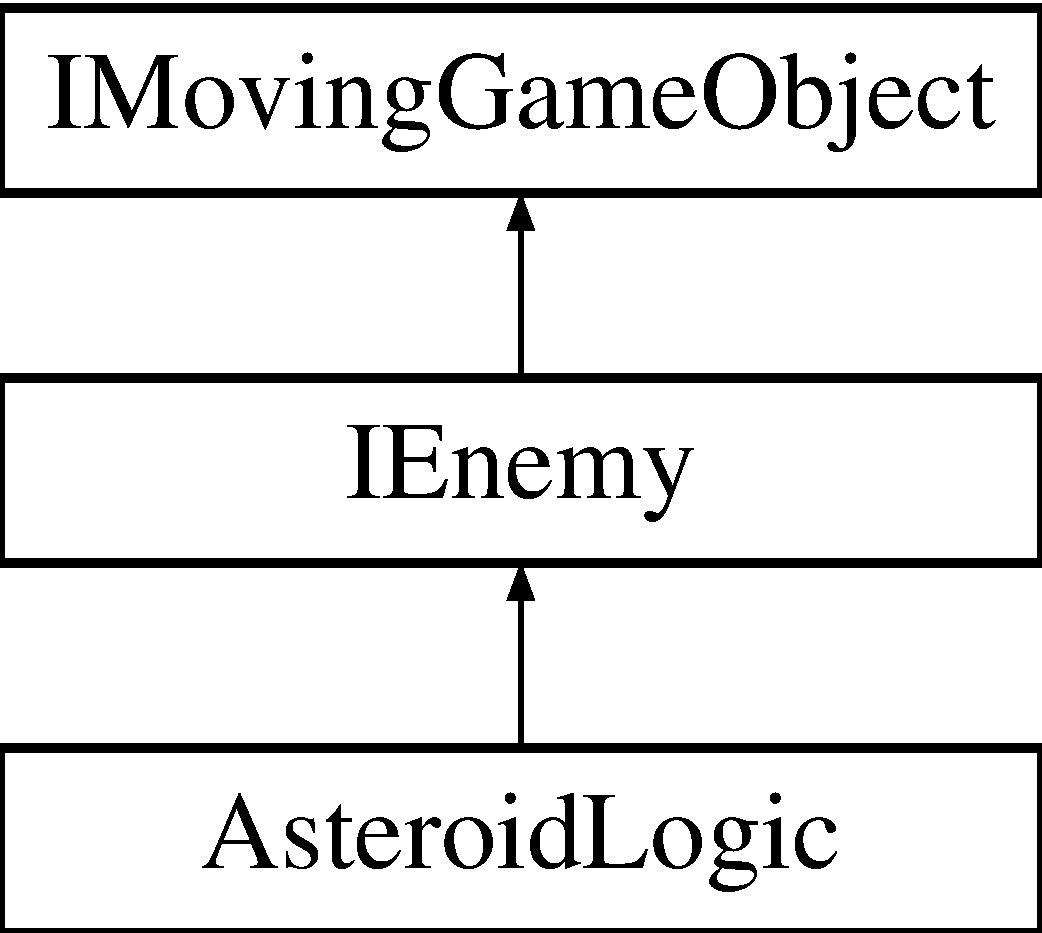
\includegraphics[height=3.000000cm]{class_asteroid_logic}
\end{center}
\end{figure}
\subsection*{Public Member Functions}
\begin{DoxyCompactItemize}
\item 
\mbox{\Hypertarget{class_asteroid_logic_af566df9981ce525a41f7ce42e49e64b0}\label{class_asteroid_logic_af566df9981ce525a41f7ce42e49e64b0}} 
{\bfseries Asteroid\+Logic} (float theta)
\item 
\mbox{\Hypertarget{class_asteroid_logic_af20b202c4f5857279192733a0b2fdbd3}\label{class_asteroid_logic_af20b202c4f5857279192733a0b2fdbd3}} 
void {\bfseries move} ()
\item 
\mbox{\Hypertarget{class_asteroid_logic_a2087d2a3b9bf9e6f1367833454b2fb97}\label{class_asteroid_logic_a2087d2a3b9bf9e6f1367833454b2fb97}} 
float {\bfseries get\+Angleof\+Rotation} ()
\item 
\mbox{\Hypertarget{class_asteroid_logic_a18e01f832db4f109799fc01c8c15efcd}\label{class_asteroid_logic_a18e01f832db4f109799fc01c8c15efcd}} 
bool {\bfseries is\+Alive} ()
\item 
\mbox{\Hypertarget{class_asteroid_logic_a54519e4b2719c70d17f5a28bb0d8fb56}\label{class_asteroid_logic_a54519e4b2719c70d17f5a28bb0d8fb56}} 
void {\bfseries reduce\+Health} (int \+\_\+damage)
\item 
\mbox{\Hypertarget{class_asteroid_logic_a1d79a614c5e1a9409404f6a2def25761}\label{class_asteroid_logic_a1d79a614c5e1a9409404f6a2def25761}} 
float {\bfseries get\+Xposition} ()
\item 
\mbox{\Hypertarget{class_asteroid_logic_a83863c5262a29b2999d04ad443622bbc}\label{class_asteroid_logic_a83863c5262a29b2999d04ad443622bbc}} 
float {\bfseries get\+Yposition} ()
\item 
\mbox{\Hypertarget{class_asteroid_logic_a594dc710574cac901e9999474b9379fe}\label{class_asteroid_logic_a594dc710574cac901e9999474b9379fe}} 
void {\bfseries set\+Life} (bool life)
\item 
\mbox{\Hypertarget{class_asteroid_logic_a575d9f801770906960b65dafe937fba5}\label{class_asteroid_logic_a575d9f801770906960b65dafe937fba5}} 
float {\bfseries get\+Radius} ()
\item 
\mbox{\Hypertarget{class_asteroid_logic_a4bff0373a2cefe48c984b469ddbcb52d}\label{class_asteroid_logic_a4bff0373a2cefe48c984b469ddbcb52d}} 
float {\bfseries get\+Center\+X\+Position} ()
\item 
\mbox{\Hypertarget{class_asteroid_logic_a00c9cda893b9dee7e2225377dd54a2eb}\label{class_asteroid_logic_a00c9cda893b9dee7e2225377dd54a2eb}} 
float {\bfseries get\+Center\+Y\+Position} ()
\item 
\mbox{\Hypertarget{class_asteroid_logic_ac9bfa7e9a3eed670f9264f15f395894e}\label{class_asteroid_logic_ac9bfa7e9a3eed670f9264f15f395894e}} 
void {\bfseries set\+Out\+Of\+Bounds} (bool bounds)
\item 
\mbox{\Hypertarget{class_asteroid_logic_ad2fadce802b18aa2d57baee65a56833e}\label{class_asteroid_logic_ad2fadce802b18aa2d57baee65a56833e}} 
bool {\bfseries is\+Out\+Of\+Bounds} ()
\item 
\mbox{\Hypertarget{class_asteroid_logic_abe3018168bb1a91b78aac410a3cb7853}\label{class_asteroid_logic_abe3018168bb1a91b78aac410a3cb7853}} 
float {\bfseries get\+Damage} ()
\end{DoxyCompactItemize}


The documentation for this class was generated from the following files\+:\begin{DoxyCompactItemize}
\item 
C\+:/\+Users/\+William/\+Documents/\+E\+L\+E\+N3009/\+Space\+Rider\+Project/Asteroid\+Logic.\+h\item 
C\+:/\+Users/\+William/\+Documents/\+E\+L\+E\+N3009/\+Space\+Rider\+Project/Asteroid\+Logic.\+cpp\end{DoxyCompactItemize}

\hypertarget{class_asteroid_presentation}{}\section{Asteroid\+Presentation Class Reference}
\label{class_asteroid_presentation}\index{Asteroid\+Presentation@{Asteroid\+Presentation}}
\subsection*{Public Member Functions}
\begin{DoxyCompactItemize}
\item 
\mbox{\Hypertarget{class_asteroid_presentation_ac35adcd9ce3dabdb0c34b8cbf14cce9c}\label{class_asteroid_presentation_ac35adcd9ce3dabdb0c34b8cbf14cce9c}} 
void {\bfseries draw} (Render\+Window \&window)
\item 
\mbox{\Hypertarget{class_asteroid_presentation_a9af9a0a566030782f33f424c633227cc}\label{class_asteroid_presentation_a9af9a0a566030782f33f424c633227cc}} 
void {\bfseries update\+Asteroid} (float x\+Position, float y\+Position)
\item 
\mbox{\Hypertarget{class_asteroid_presentation_ab1722869d573e4c6d3031033c6f74062}\label{class_asteroid_presentation_ab1722869d573e4c6d3031033c6f74062}} 
Sprite {\bfseries get\+Asteroid\+Sprite} ()
\end{DoxyCompactItemize}


The documentation for this class was generated from the following files\+:\begin{DoxyCompactItemize}
\item 
C\+:/\+Users/\+William/\+Documents/\+E\+L\+E\+N3009/\+Space\+Rider\+Project/Asteroid\+Presentation.\+h\item 
C\+:/\+Users/\+William/\+Documents/\+E\+L\+E\+N3009/\+Space\+Rider\+Project/Asteroid\+Presentation.\+cpp\end{DoxyCompactItemize}

\hypertarget{class_collision_detection}{}\section{Collision\+Detection Class Reference}
\label{class_collision_detection}\index{Collision\+Detection@{Collision\+Detection}}


{\ttfamily \#include $<$Collision\+Detection.\+h$>$}

\subsection*{Public Member Functions}
\begin{DoxyCompactItemize}
\item 
\hyperlink{class_collision_detection_ac5b8af06521eccb38b5707209fa175e2}{Collision\+Detection} ()
\item 
bool \hyperlink{class_collision_detection_a8e58e83acc7de60673126754ac2246cd}{did\+Objects\+Collide} (\hyperlink{class_i_moving_game_object}{I\+Moving\+Game\+Object} \&obj1, \hyperlink{class_i_moving_game_object}{I\+Moving\+Game\+Object} \&obj2)
\end{DoxyCompactItemize}


\subsection{Constructor \& Destructor Documentation}
\mbox{\Hypertarget{class_collision_detection_ac5b8af06521eccb38b5707209fa175e2}\label{class_collision_detection_ac5b8af06521eccb38b5707209fa175e2}} 
\index{Collision\+Detection@{Collision\+Detection}!Collision\+Detection@{Collision\+Detection}}
\index{Collision\+Detection@{Collision\+Detection}!Collision\+Detection@{Collision\+Detection}}
\subsubsection{\texorpdfstring{Collision\+Detection()}{CollisionDetection()}}
{\footnotesize\ttfamily Collision\+Detection\+::\+Collision\+Detection (\begin{DoxyParamCaption}{ }\end{DoxyParamCaption})}



\subsection{Member Function Documentation}
\mbox{\Hypertarget{class_collision_detection_a8e58e83acc7de60673126754ac2246cd}\label{class_collision_detection_a8e58e83acc7de60673126754ac2246cd}} 
\index{Collision\+Detection@{Collision\+Detection}!did\+Objects\+Collide@{did\+Objects\+Collide}}
\index{did\+Objects\+Collide@{did\+Objects\+Collide}!Collision\+Detection@{Collision\+Detection}}
\subsubsection{\texorpdfstring{did\+Objects\+Collide()}{didObjectsCollide()}}
{\footnotesize\ttfamily bool Collision\+Detection\+::did\+Objects\+Collide (\begin{DoxyParamCaption}\item[{\hyperlink{class_i_moving_game_object}{I\+Moving\+Game\+Object} \&}]{obj1,  }\item[{\hyperlink{class_i_moving_game_object}{I\+Moving\+Game\+Object} \&}]{obj2 }\end{DoxyParamCaption})}

Here is the call graph for this function\+:\nopagebreak
\begin{figure}[H]
\begin{center}
\leavevmode
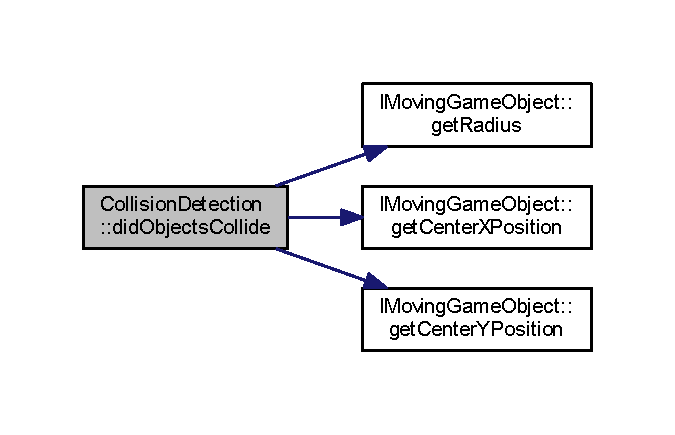
\includegraphics[width=324pt]{class_collision_detection_a8e58e83acc7de60673126754ac2246cd_cgraph}
\end{center}
\end{figure}
Here is the caller graph for this function\+:
\nopagebreak
\begin{figure}[H]
\begin{center}
\leavevmode
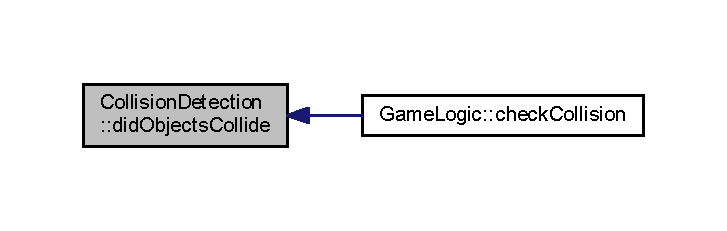
\includegraphics[width=349pt]{class_collision_detection_a8e58e83acc7de60673126754ac2246cd_icgraph}
\end{center}
\end{figure}


The documentation for this class was generated from the following files\+:\begin{DoxyCompactItemize}
\item 
C\+:/\+Users/\+User/\+Documents/\+Software\+Dev2\+Project/\+Space\+Rider\+Project/\hyperlink{_collision_detection_8h}{Collision\+Detection.\+h}\item 
C\+:/\+Users/\+User/\+Documents/\+Software\+Dev2\+Project/\+Space\+Rider\+Project/\hyperlink{_collision_detection_8cpp}{Collision\+Detection.\+cpp}\end{DoxyCompactItemize}

\hypertarget{class_enemy_bullet_logic}{}\section{Enemy\+Bullet\+Logic Class Reference}
\label{class_enemy_bullet_logic}\index{Enemy\+Bullet\+Logic@{Enemy\+Bullet\+Logic}}


{\ttfamily \#include $<$Enemy\+Bullet\+Logic.\+h$>$}



Inheritance diagram for Enemy\+Bullet\+Logic\+:\nopagebreak
\begin{figure}[H]
\begin{center}
\leavevmode
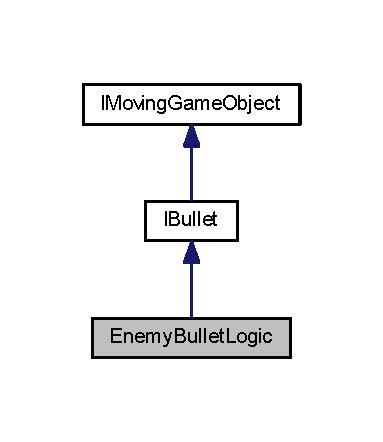
\includegraphics[width=184pt]{class_enemy_bullet_logic__inherit__graph}
\end{center}
\end{figure}


Collaboration diagram for Enemy\+Bullet\+Logic\+:\nopagebreak
\begin{figure}[H]
\begin{center}
\leavevmode
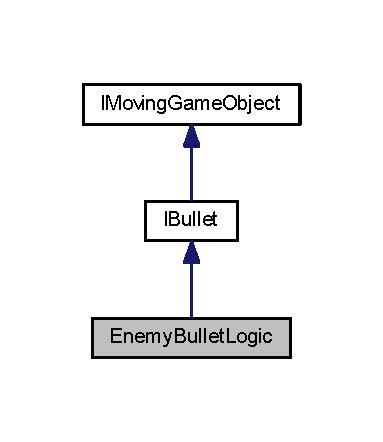
\includegraphics[width=184pt]{class_enemy_bullet_logic__coll__graph}
\end{center}
\end{figure}
\subsection*{Public Member Functions}
\begin{DoxyCompactItemize}
\item 
\hyperlink{class_enemy_bullet_logic_a0699eb27d52ed8651d611790f06e6661}{Enemy\+Bullet\+Logic} ()
\item 
\hyperlink{class_enemy_bullet_logic_a8f9f29a7c39830ccffc793adecf70c0e}{Enemy\+Bullet\+Logic} (float enemy\+X\+Position, float enemy\+Y\+Position, float theta)
\item 
void \hyperlink{class_enemy_bullet_logic_aaa5273b969347ce8c6e62261ccc3df3a}{move} ()
\item 
float \hyperlink{class_enemy_bullet_logic_afe73016d27c33171a20c15e11026106e}{get\+Xposition} ()
\item 
float \hyperlink{class_enemy_bullet_logic_a0cfb3013a7613f7f6de91a6db04d03b1}{get\+Yposition} ()
\item 
bool \hyperlink{class_enemy_bullet_logic_a42d10bdfde42178e272997de9b387398}{is\+Alive} ()
\item 
void \hyperlink{class_enemy_bullet_logic_a3e4ce40e06e9fa23826bd74015fd75f2}{set\+Damage} (int damage)
\item 
int \hyperlink{class_enemy_bullet_logic_a08dd084364fc7efc689a7f98e1cee688}{get\+Damage} ()
\item 
void \hyperlink{class_enemy_bullet_logic_a92e4dfb6a528114ad58f9ae64924fbab}{set\+Life} (bool life)
\item 
float \hyperlink{class_enemy_bullet_logic_a7e473b13bf07fdf8eb76b65e02879bf7}{get\+Radius} ()
\item 
float \hyperlink{class_enemy_bullet_logic_a39ffa8b7fabb84625a859691099652de}{get\+Center\+X\+Position} ()
\item 
float \hyperlink{class_enemy_bullet_logic_a4c006085f2a11f68e8043bca67d3effe}{get\+Center\+Y\+Position} ()
\item 
void \hyperlink{class_enemy_bullet_logic_a0263d2207f0d4332efa2cf8f8bbdc42c}{set\+Bullet\+Speed} (float speed)
\end{DoxyCompactItemize}


\subsection{Constructor \& Destructor Documentation}
\mbox{\Hypertarget{class_enemy_bullet_logic_a0699eb27d52ed8651d611790f06e6661}\label{class_enemy_bullet_logic_a0699eb27d52ed8651d611790f06e6661}} 
\index{Enemy\+Bullet\+Logic@{Enemy\+Bullet\+Logic}!Enemy\+Bullet\+Logic@{Enemy\+Bullet\+Logic}}
\index{Enemy\+Bullet\+Logic@{Enemy\+Bullet\+Logic}!Enemy\+Bullet\+Logic@{Enemy\+Bullet\+Logic}}
\subsubsection{\texorpdfstring{Enemy\+Bullet\+Logic()}{EnemyBulletLogic()}\hspace{0.1cm}{\footnotesize\ttfamily [1/2]}}
{\footnotesize\ttfamily Enemy\+Bullet\+Logic\+::\+Enemy\+Bullet\+Logic (\begin{DoxyParamCaption}{ }\end{DoxyParamCaption})}

\mbox{\Hypertarget{class_enemy_bullet_logic_a8f9f29a7c39830ccffc793adecf70c0e}\label{class_enemy_bullet_logic_a8f9f29a7c39830ccffc793adecf70c0e}} 
\index{Enemy\+Bullet\+Logic@{Enemy\+Bullet\+Logic}!Enemy\+Bullet\+Logic@{Enemy\+Bullet\+Logic}}
\index{Enemy\+Bullet\+Logic@{Enemy\+Bullet\+Logic}!Enemy\+Bullet\+Logic@{Enemy\+Bullet\+Logic}}
\subsubsection{\texorpdfstring{Enemy\+Bullet\+Logic()}{EnemyBulletLogic()}\hspace{0.1cm}{\footnotesize\ttfamily [2/2]}}
{\footnotesize\ttfamily Enemy\+Bullet\+Logic\+::\+Enemy\+Bullet\+Logic (\begin{DoxyParamCaption}\item[{float}]{enemy\+X\+Position,  }\item[{float}]{enemy\+Y\+Position,  }\item[{float}]{theta }\end{DoxyParamCaption})}



\subsection{Member Function Documentation}
\mbox{\Hypertarget{class_enemy_bullet_logic_a39ffa8b7fabb84625a859691099652de}\label{class_enemy_bullet_logic_a39ffa8b7fabb84625a859691099652de}} 
\index{Enemy\+Bullet\+Logic@{Enemy\+Bullet\+Logic}!get\+Center\+X\+Position@{get\+Center\+X\+Position}}
\index{get\+Center\+X\+Position@{get\+Center\+X\+Position}!Enemy\+Bullet\+Logic@{Enemy\+Bullet\+Logic}}
\subsubsection{\texorpdfstring{get\+Center\+X\+Position()}{getCenterXPosition()}}
{\footnotesize\ttfamily float Enemy\+Bullet\+Logic\+::get\+Center\+X\+Position (\begin{DoxyParamCaption}{ }\end{DoxyParamCaption})\hspace{0.3cm}{\ttfamily [virtual]}}



Implements \hyperlink{class_i_bullet_a43a43e2df81e05a03be42d9025e6dd2a}{I\+Bullet}.

\mbox{\Hypertarget{class_enemy_bullet_logic_a4c006085f2a11f68e8043bca67d3effe}\label{class_enemy_bullet_logic_a4c006085f2a11f68e8043bca67d3effe}} 
\index{Enemy\+Bullet\+Logic@{Enemy\+Bullet\+Logic}!get\+Center\+Y\+Position@{get\+Center\+Y\+Position}}
\index{get\+Center\+Y\+Position@{get\+Center\+Y\+Position}!Enemy\+Bullet\+Logic@{Enemy\+Bullet\+Logic}}
\subsubsection{\texorpdfstring{get\+Center\+Y\+Position()}{getCenterYPosition()}}
{\footnotesize\ttfamily float Enemy\+Bullet\+Logic\+::get\+Center\+Y\+Position (\begin{DoxyParamCaption}{ }\end{DoxyParamCaption})\hspace{0.3cm}{\ttfamily [virtual]}}



Implements \hyperlink{class_i_bullet_a8245ed2bc72beed1d69547ce5f87a021}{I\+Bullet}.

\mbox{\Hypertarget{class_enemy_bullet_logic_a08dd084364fc7efc689a7f98e1cee688}\label{class_enemy_bullet_logic_a08dd084364fc7efc689a7f98e1cee688}} 
\index{Enemy\+Bullet\+Logic@{Enemy\+Bullet\+Logic}!get\+Damage@{get\+Damage}}
\index{get\+Damage@{get\+Damage}!Enemy\+Bullet\+Logic@{Enemy\+Bullet\+Logic}}
\subsubsection{\texorpdfstring{get\+Damage()}{getDamage()}}
{\footnotesize\ttfamily int Enemy\+Bullet\+Logic\+::get\+Damage (\begin{DoxyParamCaption}{ }\end{DoxyParamCaption})\hspace{0.3cm}{\ttfamily [virtual]}}



Implements \hyperlink{class_i_bullet_ab6643a4ad3888ee4ebfbc3d445c4b73d}{I\+Bullet}.

\mbox{\Hypertarget{class_enemy_bullet_logic_a7e473b13bf07fdf8eb76b65e02879bf7}\label{class_enemy_bullet_logic_a7e473b13bf07fdf8eb76b65e02879bf7}} 
\index{Enemy\+Bullet\+Logic@{Enemy\+Bullet\+Logic}!get\+Radius@{get\+Radius}}
\index{get\+Radius@{get\+Radius}!Enemy\+Bullet\+Logic@{Enemy\+Bullet\+Logic}}
\subsubsection{\texorpdfstring{get\+Radius()}{getRadius()}}
{\footnotesize\ttfamily float Enemy\+Bullet\+Logic\+::get\+Radius (\begin{DoxyParamCaption}{ }\end{DoxyParamCaption})\hspace{0.3cm}{\ttfamily [virtual]}}



Implements \hyperlink{class_i_bullet_a327968e71126cdea5998076d8919354f}{I\+Bullet}.

\mbox{\Hypertarget{class_enemy_bullet_logic_afe73016d27c33171a20c15e11026106e}\label{class_enemy_bullet_logic_afe73016d27c33171a20c15e11026106e}} 
\index{Enemy\+Bullet\+Logic@{Enemy\+Bullet\+Logic}!get\+Xposition@{get\+Xposition}}
\index{get\+Xposition@{get\+Xposition}!Enemy\+Bullet\+Logic@{Enemy\+Bullet\+Logic}}
\subsubsection{\texorpdfstring{get\+Xposition()}{getXposition()}}
{\footnotesize\ttfamily float Enemy\+Bullet\+Logic\+::get\+Xposition (\begin{DoxyParamCaption}{ }\end{DoxyParamCaption})\hspace{0.3cm}{\ttfamily [virtual]}}



Implements \hyperlink{class_i_bullet_a20babdd6c657ddda175e84a56564dcfa}{I\+Bullet}.

\mbox{\Hypertarget{class_enemy_bullet_logic_a0cfb3013a7613f7f6de91a6db04d03b1}\label{class_enemy_bullet_logic_a0cfb3013a7613f7f6de91a6db04d03b1}} 
\index{Enemy\+Bullet\+Logic@{Enemy\+Bullet\+Logic}!get\+Yposition@{get\+Yposition}}
\index{get\+Yposition@{get\+Yposition}!Enemy\+Bullet\+Logic@{Enemy\+Bullet\+Logic}}
\subsubsection{\texorpdfstring{get\+Yposition()}{getYposition()}}
{\footnotesize\ttfamily float Enemy\+Bullet\+Logic\+::get\+Yposition (\begin{DoxyParamCaption}{ }\end{DoxyParamCaption})\hspace{0.3cm}{\ttfamily [virtual]}}



Implements \hyperlink{class_i_bullet_a36594de9a0c0ddd7083bca10ef5d8332}{I\+Bullet}.

\mbox{\Hypertarget{class_enemy_bullet_logic_a42d10bdfde42178e272997de9b387398}\label{class_enemy_bullet_logic_a42d10bdfde42178e272997de9b387398}} 
\index{Enemy\+Bullet\+Logic@{Enemy\+Bullet\+Logic}!is\+Alive@{is\+Alive}}
\index{is\+Alive@{is\+Alive}!Enemy\+Bullet\+Logic@{Enemy\+Bullet\+Logic}}
\subsubsection{\texorpdfstring{is\+Alive()}{isAlive()}}
{\footnotesize\ttfamily bool Enemy\+Bullet\+Logic\+::is\+Alive (\begin{DoxyParamCaption}{ }\end{DoxyParamCaption})\hspace{0.3cm}{\ttfamily [virtual]}}



Implements \hyperlink{class_i_bullet_ac1252496738126ec94a97512011b9112}{I\+Bullet}.

\mbox{\Hypertarget{class_enemy_bullet_logic_aaa5273b969347ce8c6e62261ccc3df3a}\label{class_enemy_bullet_logic_aaa5273b969347ce8c6e62261ccc3df3a}} 
\index{Enemy\+Bullet\+Logic@{Enemy\+Bullet\+Logic}!move@{move}}
\index{move@{move}!Enemy\+Bullet\+Logic@{Enemy\+Bullet\+Logic}}
\subsubsection{\texorpdfstring{move()}{move()}}
{\footnotesize\ttfamily void Enemy\+Bullet\+Logic\+::move (\begin{DoxyParamCaption}{ }\end{DoxyParamCaption})\hspace{0.3cm}{\ttfamily [virtual]}}



Implements \hyperlink{class_i_bullet_a0884074f0bc793fb5a52ac33842622fd}{I\+Bullet}.

\mbox{\Hypertarget{class_enemy_bullet_logic_a0263d2207f0d4332efa2cf8f8bbdc42c}\label{class_enemy_bullet_logic_a0263d2207f0d4332efa2cf8f8bbdc42c}} 
\index{Enemy\+Bullet\+Logic@{Enemy\+Bullet\+Logic}!set\+Bullet\+Speed@{set\+Bullet\+Speed}}
\index{set\+Bullet\+Speed@{set\+Bullet\+Speed}!Enemy\+Bullet\+Logic@{Enemy\+Bullet\+Logic}}
\subsubsection{\texorpdfstring{set\+Bullet\+Speed()}{setBulletSpeed()}}
{\footnotesize\ttfamily void Enemy\+Bullet\+Logic\+::set\+Bullet\+Speed (\begin{DoxyParamCaption}\item[{float}]{speed }\end{DoxyParamCaption})}

Here is the caller graph for this function\+:\nopagebreak
\begin{figure}[H]
\begin{center}
\leavevmode
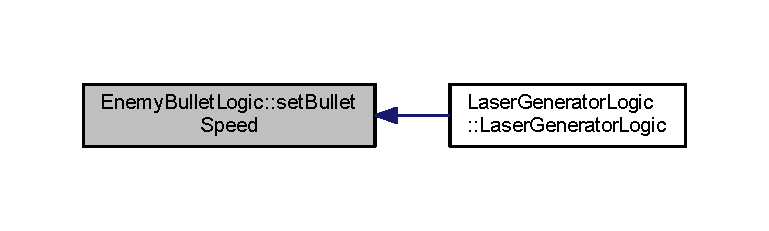
\includegraphics[width=350pt]{class_enemy_bullet_logic_a0263d2207f0d4332efa2cf8f8bbdc42c_icgraph}
\end{center}
\end{figure}
\mbox{\Hypertarget{class_enemy_bullet_logic_a3e4ce40e06e9fa23826bd74015fd75f2}\label{class_enemy_bullet_logic_a3e4ce40e06e9fa23826bd74015fd75f2}} 
\index{Enemy\+Bullet\+Logic@{Enemy\+Bullet\+Logic}!set\+Damage@{set\+Damage}}
\index{set\+Damage@{set\+Damage}!Enemy\+Bullet\+Logic@{Enemy\+Bullet\+Logic}}
\subsubsection{\texorpdfstring{set\+Damage()}{setDamage()}}
{\footnotesize\ttfamily void Enemy\+Bullet\+Logic\+::set\+Damage (\begin{DoxyParamCaption}\item[{int}]{damage }\end{DoxyParamCaption})\hspace{0.3cm}{\ttfamily [virtual]}}



Implements \hyperlink{class_i_bullet_a072298555accb47f11b84f4c781ae876}{I\+Bullet}.

Here is the caller graph for this function\+:\nopagebreak
\begin{figure}[H]
\begin{center}
\leavevmode
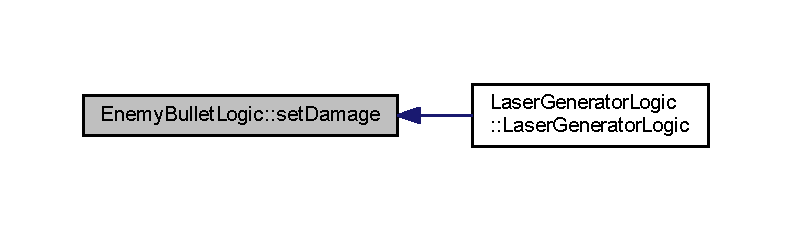
\includegraphics[width=350pt]{class_enemy_bullet_logic_a3e4ce40e06e9fa23826bd74015fd75f2_icgraph}
\end{center}
\end{figure}
\mbox{\Hypertarget{class_enemy_bullet_logic_a92e4dfb6a528114ad58f9ae64924fbab}\label{class_enemy_bullet_logic_a92e4dfb6a528114ad58f9ae64924fbab}} 
\index{Enemy\+Bullet\+Logic@{Enemy\+Bullet\+Logic}!set\+Life@{set\+Life}}
\index{set\+Life@{set\+Life}!Enemy\+Bullet\+Logic@{Enemy\+Bullet\+Logic}}
\subsubsection{\texorpdfstring{set\+Life()}{setLife()}}
{\footnotesize\ttfamily void Enemy\+Bullet\+Logic\+::set\+Life (\begin{DoxyParamCaption}\item[{bool}]{life }\end{DoxyParamCaption})\hspace{0.3cm}{\ttfamily [virtual]}}



Implements \hyperlink{class_i_bullet_abf99befdaa121e7c9ca2acc2ed75b513}{I\+Bullet}.



The documentation for this class was generated from the following files\+:\begin{DoxyCompactItemize}
\item 
C\+:/\+Users/\+User/\+Documents/\+Software\+Dev2\+Project/\+Space\+Rider\+Project/\hyperlink{_enemy_bullet_logic_8h}{Enemy\+Bullet\+Logic.\+h}\item 
C\+:/\+Users/\+User/\+Documents/\+Software\+Dev2\+Project/\+Space\+Rider\+Project/\hyperlink{_enemy_bullet_logic_8cpp}{Enemy\+Bullet\+Logic.\+cpp}\end{DoxyCompactItemize}

\hypertarget{class_enemy_bullet_presentation}{}\section{Enemy\+Bullet\+Presentation Class Reference}
\label{class_enemy_bullet_presentation}\index{Enemy\+Bullet\+Presentation@{Enemy\+Bullet\+Presentation}}


{\ttfamily \#include $<$Enemy\+Bullet\+Presentation.\+h$>$}

\subsection*{Public Member Functions}
\begin{DoxyCompactItemize}
\item 
\hyperlink{class_enemy_bullet_presentation_a9f2f47470f74f7c2f0df928ad3307e29}{Enemy\+Bullet\+Presentation} ()
\item 
\hyperlink{class_enemy_bullet_presentation_a650d6adb9afd73ec43d91791919e9797}{Enemy\+Bullet\+Presentation} (float x\+Position, float y\+Position)
\item 
void \hyperlink{class_enemy_bullet_presentation_ab47308a4c94cd9ee4c16f0b528a9c77b}{draw} (Render\+Window \&window)
\item 
void \hyperlink{class_enemy_bullet_presentation_a89cf545e80590e548f9f32dcce8edc98}{update\+Enemy\+Bullet} (float x\+Position, float y\+Position)
\item 
Circle\+Shape \hyperlink{class_enemy_bullet_presentation_a38b81cebcff8e858e6cbaf8df7a6fa23}{get\+Enemy\+Bullet} ()
\end{DoxyCompactItemize}


\subsection{Constructor \& Destructor Documentation}
\mbox{\Hypertarget{class_enemy_bullet_presentation_a9f2f47470f74f7c2f0df928ad3307e29}\label{class_enemy_bullet_presentation_a9f2f47470f74f7c2f0df928ad3307e29}} 
\index{Enemy\+Bullet\+Presentation@{Enemy\+Bullet\+Presentation}!Enemy\+Bullet\+Presentation@{Enemy\+Bullet\+Presentation}}
\index{Enemy\+Bullet\+Presentation@{Enemy\+Bullet\+Presentation}!Enemy\+Bullet\+Presentation@{Enemy\+Bullet\+Presentation}}
\subsubsection{\texorpdfstring{Enemy\+Bullet\+Presentation()}{EnemyBulletPresentation()}\hspace{0.1cm}{\footnotesize\ttfamily [1/2]}}
{\footnotesize\ttfamily Enemy\+Bullet\+Presentation\+::\+Enemy\+Bullet\+Presentation (\begin{DoxyParamCaption}{ }\end{DoxyParamCaption})}

\mbox{\Hypertarget{class_enemy_bullet_presentation_a650d6adb9afd73ec43d91791919e9797}\label{class_enemy_bullet_presentation_a650d6adb9afd73ec43d91791919e9797}} 
\index{Enemy\+Bullet\+Presentation@{Enemy\+Bullet\+Presentation}!Enemy\+Bullet\+Presentation@{Enemy\+Bullet\+Presentation}}
\index{Enemy\+Bullet\+Presentation@{Enemy\+Bullet\+Presentation}!Enemy\+Bullet\+Presentation@{Enemy\+Bullet\+Presentation}}
\subsubsection{\texorpdfstring{Enemy\+Bullet\+Presentation()}{EnemyBulletPresentation()}\hspace{0.1cm}{\footnotesize\ttfamily [2/2]}}
{\footnotesize\ttfamily Enemy\+Bullet\+Presentation\+::\+Enemy\+Bullet\+Presentation (\begin{DoxyParamCaption}\item[{float}]{x\+Position,  }\item[{float}]{y\+Position }\end{DoxyParamCaption})}



\subsection{Member Function Documentation}
\mbox{\Hypertarget{class_enemy_bullet_presentation_ab47308a4c94cd9ee4c16f0b528a9c77b}\label{class_enemy_bullet_presentation_ab47308a4c94cd9ee4c16f0b528a9c77b}} 
\index{Enemy\+Bullet\+Presentation@{Enemy\+Bullet\+Presentation}!draw@{draw}}
\index{draw@{draw}!Enemy\+Bullet\+Presentation@{Enemy\+Bullet\+Presentation}}
\subsubsection{\texorpdfstring{draw()}{draw()}}
{\footnotesize\ttfamily void Enemy\+Bullet\+Presentation\+::draw (\begin{DoxyParamCaption}\item[{Render\+Window \&}]{window }\end{DoxyParamCaption})}

\mbox{\Hypertarget{class_enemy_bullet_presentation_a38b81cebcff8e858e6cbaf8df7a6fa23}\label{class_enemy_bullet_presentation_a38b81cebcff8e858e6cbaf8df7a6fa23}} 
\index{Enemy\+Bullet\+Presentation@{Enemy\+Bullet\+Presentation}!get\+Enemy\+Bullet@{get\+Enemy\+Bullet}}
\index{get\+Enemy\+Bullet@{get\+Enemy\+Bullet}!Enemy\+Bullet\+Presentation@{Enemy\+Bullet\+Presentation}}
\subsubsection{\texorpdfstring{get\+Enemy\+Bullet()}{getEnemyBullet()}}
{\footnotesize\ttfamily Circle\+Shape Enemy\+Bullet\+Presentation\+::get\+Enemy\+Bullet (\begin{DoxyParamCaption}{ }\end{DoxyParamCaption})}

\mbox{\Hypertarget{class_enemy_bullet_presentation_a89cf545e80590e548f9f32dcce8edc98}\label{class_enemy_bullet_presentation_a89cf545e80590e548f9f32dcce8edc98}} 
\index{Enemy\+Bullet\+Presentation@{Enemy\+Bullet\+Presentation}!update\+Enemy\+Bullet@{update\+Enemy\+Bullet}}
\index{update\+Enemy\+Bullet@{update\+Enemy\+Bullet}!Enemy\+Bullet\+Presentation@{Enemy\+Bullet\+Presentation}}
\subsubsection{\texorpdfstring{update\+Enemy\+Bullet()}{updateEnemyBullet()}}
{\footnotesize\ttfamily void Enemy\+Bullet\+Presentation\+::update\+Enemy\+Bullet (\begin{DoxyParamCaption}\item[{float}]{x\+Position,  }\item[{float}]{y\+Position }\end{DoxyParamCaption})}



The documentation for this class was generated from the following files\+:\begin{DoxyCompactItemize}
\item 
C\+:/\+Users/\+User/\+Documents/\+Software\+Dev2\+Project/\+Space\+Rider\+Project/\hyperlink{_enemy_bullet_presentation_8h}{Enemy\+Bullet\+Presentation.\+h}\item 
C\+:/\+Users/\+User/\+Documents/\+Software\+Dev2\+Project/\+Space\+Rider\+Project/\hyperlink{_enemy_bullet_presentation_8cpp}{Enemy\+Bullet\+Presentation.\+cpp}\end{DoxyCompactItemize}

\hypertarget{class_enemy_logic}{}\section{Enemy\+Logic Class Reference}
\label{class_enemy_logic}\index{Enemy\+Logic@{Enemy\+Logic}}
Inheritance diagram for Enemy\+Logic\+:\begin{figure}[H]
\begin{center}
\leavevmode
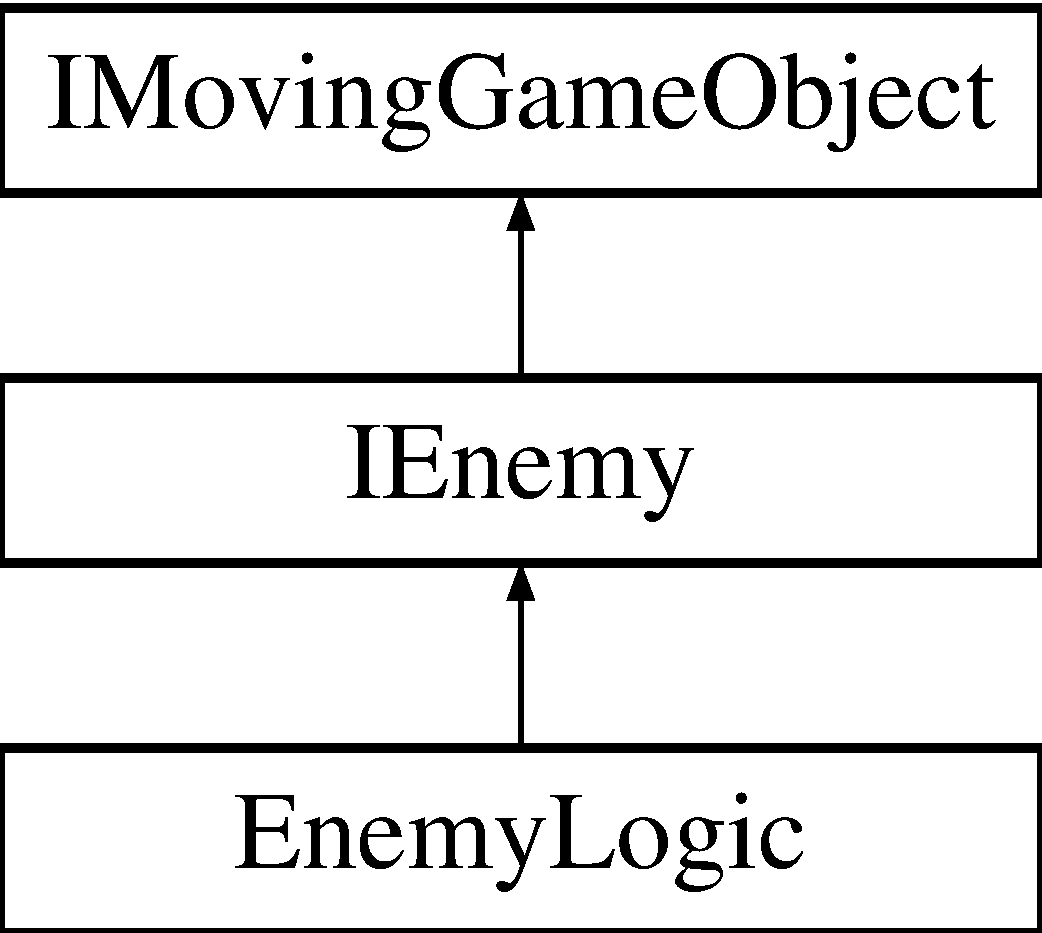
\includegraphics[height=3.000000cm]{class_enemy_logic}
\end{center}
\end{figure}
\subsection*{Public Member Functions}
\begin{DoxyCompactItemize}
\item 
\hyperlink{class_enemy_logic_a6b405895fa7556810b8002b0d276d6cc}{Enemy\+Logic} (int inital\+Xposition, int inital\+Yposition, float theta)
\begin{DoxyCompactList}\small\item\em Constructor intitializes the enemy to position and a direction angle. \end{DoxyCompactList}\item 
\mbox{\Hypertarget{class_enemy_logic_a2bc8ba642d677ab31f4b54ec00299e25}\label{class_enemy_logic_a2bc8ba642d677ab31f4b54ec00299e25}} 
void \hyperlink{class_enemy_logic_a2bc8ba642d677ab31f4b54ec00299e25}{move} ()
\begin{DoxyCompactList}\small\item\em Moves the enemy in the direction of the angle it is initialized to. \end{DoxyCompactList}\item 
float \hyperlink{class_enemy_logic_ade03be41505c71de49f20fc855c8fede}{get\+Angleof\+Rotation} ()
\begin{DoxyCompactList}\small\item\em Returns the angle of rotation of the enemy. \end{DoxyCompactList}\item 
bool \hyperlink{class_enemy_logic_a8dd48fa112c41249e46728d7ec8f820e}{is\+Alive} ()
\begin{DoxyCompactList}\small\item\em Returns true if the enemy\textquotesingle{}s health is greater than zero. \end{DoxyCompactList}\item 
void \hyperlink{class_enemy_logic_aaf2f8ff785c8f7410e04cfb3cb192b9b}{reduce\+Health} (int \+\_\+damage)
\begin{DoxyCompactList}\small\item\em Decreases the health of the enemy by an amount given by the parameteter. \end{DoxyCompactList}\item 
float \hyperlink{class_enemy_logic_a7eed969ab8e3d2527cdac04ef39a5aba}{get\+Xposition} ()
\begin{DoxyCompactList}\small\item\em Returns the x co-\/ordinate of the enemy. \end{DoxyCompactList}\item 
float \hyperlink{class_enemy_logic_ae614032054926a4a25ed56f61111392b}{get\+Yposition} ()
\begin{DoxyCompactList}\small\item\em Returns the y co-\/ordinate of the enemy. \end{DoxyCompactList}\item 
void \hyperlink{class_enemy_logic_a12bce0a6b6cad1af96aee3b401ea2c45}{set\+Life} (bool life)
\begin{DoxyCompactList}\small\item\em Sets the enemy\textquotesingle{}s life status to dead or alive according to the parameter. \end{DoxyCompactList}\item 
bool \hyperlink{class_enemy_logic_a2e3e9e006259b36745beff4b55fd9bdc}{is\+Out\+Of\+Bounds} ()
\begin{DoxyCompactList}\small\item\em Returns the out\+Of\+Bounds status of the enemy. out\+Of\+Bounds is defined by the enemy mving outside of the screen. \end{DoxyCompactList}\item 
void \hyperlink{class_enemy_logic_a0ac79ee7c0acf99b27aa4e22f98ce2d1}{set\+Outof\+Bounds} (bool out\+Of\+Bounds)
\begin{DoxyCompactList}\small\item\em Sets the outbounds status of the enemy to the out\+Of\+Bounds parameter. \end{DoxyCompactList}\item 
void \hyperlink{class_enemy_logic_a560cc578db8a77f250b63a111f51125e}{move\+To\+Center} (float x\+Position, float y\+Position, float theta)
\begin{DoxyCompactList}\small\item\em Moves the enemy to the center\+Position of the screen and sets the angle of direction for the enemy to move. \end{DoxyCompactList}\item 
float \hyperlink{class_enemy_logic_ab6736c870e69bc20bef8d6d010946eb2}{get\+Radius} ()
\begin{DoxyCompactList}\small\item\em Returns the radius of the enemy. \end{DoxyCompactList}\item 
float \hyperlink{class_enemy_logic_a1429e91a81da7646d9b0280f26519d8c}{get\+Center\+X\+Position} ()
\begin{DoxyCompactList}\small\item\em Returns the center x co-\/ordinate of the enemy\textquotesingle{}s current position. \end{DoxyCompactList}\item 
float \hyperlink{class_enemy_logic_a8eb47a87a47288783e0c8963c39d24e4}{get\+Center\+Y\+Position} ()
\begin{DoxyCompactList}\small\item\em Returns the center y co-\/ordinate of the enemy\textquotesingle{}s current position. \end{DoxyCompactList}\item 
void \hyperlink{class_enemy_logic_aae66ecc1d28feaef7c814a0dff7eed95}{set\+Enemy\+Speed} (float speed)
\begin{DoxyCompactList}\small\item\em Sets the enemy\textquotesingle{}s Speed. \end{DoxyCompactList}\item 
void \hyperlink{class_enemy_logic_acabb2cb226edc71300ba1f2bc3e7a577}{set\+Radius} (int radius)
\begin{DoxyCompactList}\small\item\em Sets the enemy\textquotesingle{}s radius. \end{DoxyCompactList}\item 
vector$<$ \hyperlink{class_enemy_bullet_logic}{Enemy\+Bullet\+Logic} $>$ \hyperlink{class_enemy_logic_ae4e49b9f854bc0407510de8e3824c7c4}{get\+Enemy\+Bullet\+Logic\+Vector} ()
\begin{DoxyCompactList}\small\item\em Returns a vector of type \hyperlink{class_enemy_bullet_logic}{Enemy\+Bullet\+Logic}. \end{DoxyCompactList}\item 
\mbox{\Hypertarget{class_enemy_logic_af85aebe59b9cdee37bdab690fa496348}\label{class_enemy_logic_af85aebe59b9cdee37bdab690fa496348}} 
void \hyperlink{class_enemy_logic_af85aebe59b9cdee37bdab690fa496348}{clear\+Enemy\+Bullet\+Vector} ()
\begin{DoxyCompactList}\small\item\em Clears the Enemy\+Bulle\+Vector. \end{DoxyCompactList}\item 
void \hyperlink{class_enemy_logic_a88584f95e49bfd6b174b9b1d9a274cc5}{set\+Enemy\+Bullet\+Life} (bool life)
\begin{DoxyCompactList}\small\item\em Sets the enemy bullets life to alive or dead. A bullets life is defined to be dead after collision and alive if it hasnt collided with a game object. \end{DoxyCompactList}\end{DoxyCompactItemize}


\subsection{Constructor \& Destructor Documentation}
\mbox{\Hypertarget{class_enemy_logic_a6b405895fa7556810b8002b0d276d6cc}\label{class_enemy_logic_a6b405895fa7556810b8002b0d276d6cc}} 
\index{Enemy\+Logic@{Enemy\+Logic}!Enemy\+Logic@{Enemy\+Logic}}
\index{Enemy\+Logic@{Enemy\+Logic}!Enemy\+Logic@{Enemy\+Logic}}
\subsubsection{\texorpdfstring{Enemy\+Logic()}{EnemyLogic()}}
{\footnotesize\ttfamily Enemy\+Logic\+::\+Enemy\+Logic (\begin{DoxyParamCaption}\item[{int}]{inital\+Xposition,  }\item[{int}]{inital\+Yposition,  }\item[{float}]{theta }\end{DoxyParamCaption})}



Constructor intitializes the enemy to position and a direction angle. 


\begin{DoxyParams}{Parameters}
{\em inital\+Xposition} & the x-\/cordinate of initial position. \\
\hline
{\em inital\+Yposition} & the y-\/cordinate of initial position. \\
\hline
{\em theta} & the angle of direction the enemy moves to. \\
\hline
\end{DoxyParams}


\subsection{Member Function Documentation}
\mbox{\Hypertarget{class_enemy_logic_ade03be41505c71de49f20fc855c8fede}\label{class_enemy_logic_ade03be41505c71de49f20fc855c8fede}} 
\index{Enemy\+Logic@{Enemy\+Logic}!get\+Angleof\+Rotation@{get\+Angleof\+Rotation}}
\index{get\+Angleof\+Rotation@{get\+Angleof\+Rotation}!Enemy\+Logic@{Enemy\+Logic}}
\subsubsection{\texorpdfstring{get\+Angleof\+Rotation()}{getAngleofRotation()}}
{\footnotesize\ttfamily float Enemy\+Logic\+::get\+Angleof\+Rotation (\begin{DoxyParamCaption}{ }\end{DoxyParamCaption})\hspace{0.3cm}{\ttfamily [virtual]}}



Returns the angle of rotation of the enemy. 

\begin{DoxyReturn}{Returns}
float containing the angle of rotation of the enemy. 
\end{DoxyReturn}


Implements \hyperlink{class_i_enemy}{I\+Enemy}.

\mbox{\Hypertarget{class_enemy_logic_a1429e91a81da7646d9b0280f26519d8c}\label{class_enemy_logic_a1429e91a81da7646d9b0280f26519d8c}} 
\index{Enemy\+Logic@{Enemy\+Logic}!get\+Center\+X\+Position@{get\+Center\+X\+Position}}
\index{get\+Center\+X\+Position@{get\+Center\+X\+Position}!Enemy\+Logic@{Enemy\+Logic}}
\subsubsection{\texorpdfstring{get\+Center\+X\+Position()}{getCenterXPosition()}}
{\footnotesize\ttfamily float Enemy\+Logic\+::get\+Center\+X\+Position (\begin{DoxyParamCaption}{ }\end{DoxyParamCaption})\hspace{0.3cm}{\ttfamily [virtual]}}



Returns the center x co-\/ordinate of the enemy\textquotesingle{}s current position. 

\begin{DoxyReturn}{Returns}
float containing enemy\textquotesingle{}s x co-\/ordinate of the center. 
\end{DoxyReturn}


Implements \hyperlink{class_i_enemy}{I\+Enemy}.

\mbox{\Hypertarget{class_enemy_logic_a8eb47a87a47288783e0c8963c39d24e4}\label{class_enemy_logic_a8eb47a87a47288783e0c8963c39d24e4}} 
\index{Enemy\+Logic@{Enemy\+Logic}!get\+Center\+Y\+Position@{get\+Center\+Y\+Position}}
\index{get\+Center\+Y\+Position@{get\+Center\+Y\+Position}!Enemy\+Logic@{Enemy\+Logic}}
\subsubsection{\texorpdfstring{get\+Center\+Y\+Position()}{getCenterYPosition()}}
{\footnotesize\ttfamily float Enemy\+Logic\+::get\+Center\+Y\+Position (\begin{DoxyParamCaption}{ }\end{DoxyParamCaption})\hspace{0.3cm}{\ttfamily [virtual]}}



Returns the center y co-\/ordinate of the enemy\textquotesingle{}s current position. 

\begin{DoxyReturn}{Returns}
float containing enemy\textquotesingle{}s y co-\/ordinate of the center. 
\end{DoxyReturn}


Implements \hyperlink{class_i_enemy}{I\+Enemy}.

\mbox{\Hypertarget{class_enemy_logic_ae4e49b9f854bc0407510de8e3824c7c4}\label{class_enemy_logic_ae4e49b9f854bc0407510de8e3824c7c4}} 
\index{Enemy\+Logic@{Enemy\+Logic}!get\+Enemy\+Bullet\+Logic\+Vector@{get\+Enemy\+Bullet\+Logic\+Vector}}
\index{get\+Enemy\+Bullet\+Logic\+Vector@{get\+Enemy\+Bullet\+Logic\+Vector}!Enemy\+Logic@{Enemy\+Logic}}
\subsubsection{\texorpdfstring{get\+Enemy\+Bullet\+Logic\+Vector()}{getEnemyBulletLogicVector()}}
{\footnotesize\ttfamily vector$<$ \hyperlink{class_enemy_bullet_logic}{Enemy\+Bullet\+Logic} $>$ Enemy\+Logic\+::get\+Enemy\+Bullet\+Logic\+Vector (\begin{DoxyParamCaption}{ }\end{DoxyParamCaption})}



Returns a vector of type \hyperlink{class_enemy_bullet_logic}{Enemy\+Bullet\+Logic}. 

\begin{DoxyReturn}{Returns}
\hyperlink{class_enemy_bullet_logic}{Enemy\+Bullet\+Logic} containing the bullets the enemy fires 
\end{DoxyReturn}
\mbox{\Hypertarget{class_enemy_logic_ab6736c870e69bc20bef8d6d010946eb2}\label{class_enemy_logic_ab6736c870e69bc20bef8d6d010946eb2}} 
\index{Enemy\+Logic@{Enemy\+Logic}!get\+Radius@{get\+Radius}}
\index{get\+Radius@{get\+Radius}!Enemy\+Logic@{Enemy\+Logic}}
\subsubsection{\texorpdfstring{get\+Radius()}{getRadius()}}
{\footnotesize\ttfamily float Enemy\+Logic\+::get\+Radius (\begin{DoxyParamCaption}{ }\end{DoxyParamCaption})\hspace{0.3cm}{\ttfamily [virtual]}}



Returns the radius of the enemy. 

\begin{DoxyReturn}{Returns}
float containing enemy\textquotesingle{}s radius. 
\end{DoxyReturn}


Implements \hyperlink{class_i_enemy}{I\+Enemy}.

\mbox{\Hypertarget{class_enemy_logic_a7eed969ab8e3d2527cdac04ef39a5aba}\label{class_enemy_logic_a7eed969ab8e3d2527cdac04ef39a5aba}} 
\index{Enemy\+Logic@{Enemy\+Logic}!get\+Xposition@{get\+Xposition}}
\index{get\+Xposition@{get\+Xposition}!Enemy\+Logic@{Enemy\+Logic}}
\subsubsection{\texorpdfstring{get\+Xposition()}{getXposition()}}
{\footnotesize\ttfamily float Enemy\+Logic\+::get\+Xposition (\begin{DoxyParamCaption}{ }\end{DoxyParamCaption})\hspace{0.3cm}{\ttfamily [virtual]}}



Returns the x co-\/ordinate of the enemy. 

\begin{DoxyReturn}{Returns}
float containing the x co-\/ordinate of the enemy. 
\end{DoxyReturn}


Implements \hyperlink{class_i_enemy}{I\+Enemy}.

\mbox{\Hypertarget{class_enemy_logic_ae614032054926a4a25ed56f61111392b}\label{class_enemy_logic_ae614032054926a4a25ed56f61111392b}} 
\index{Enemy\+Logic@{Enemy\+Logic}!get\+Yposition@{get\+Yposition}}
\index{get\+Yposition@{get\+Yposition}!Enemy\+Logic@{Enemy\+Logic}}
\subsubsection{\texorpdfstring{get\+Yposition()}{getYposition()}}
{\footnotesize\ttfamily float Enemy\+Logic\+::get\+Yposition (\begin{DoxyParamCaption}{ }\end{DoxyParamCaption})\hspace{0.3cm}{\ttfamily [virtual]}}



Returns the y co-\/ordinate of the enemy. 

\begin{DoxyReturn}{Returns}
float containing the y co-\/ordinate of the enemy 
\end{DoxyReturn}


Implements \hyperlink{class_i_enemy}{I\+Enemy}.

\mbox{\Hypertarget{class_enemy_logic_a8dd48fa112c41249e46728d7ec8f820e}\label{class_enemy_logic_a8dd48fa112c41249e46728d7ec8f820e}} 
\index{Enemy\+Logic@{Enemy\+Logic}!is\+Alive@{is\+Alive}}
\index{is\+Alive@{is\+Alive}!Enemy\+Logic@{Enemy\+Logic}}
\subsubsection{\texorpdfstring{is\+Alive()}{isAlive()}}
{\footnotesize\ttfamily bool Enemy\+Logic\+::is\+Alive (\begin{DoxyParamCaption}{ }\end{DoxyParamCaption})\hspace{0.3cm}{\ttfamily [virtual]}}



Returns true if the enemy\textquotesingle{}s health is greater than zero. 

\begin{DoxyReturn}{Returns}
boolean constaining life status of the enemy. 
\end{DoxyReturn}


Implements \hyperlink{class_i_enemy}{I\+Enemy}.

\mbox{\Hypertarget{class_enemy_logic_a2e3e9e006259b36745beff4b55fd9bdc}\label{class_enemy_logic_a2e3e9e006259b36745beff4b55fd9bdc}} 
\index{Enemy\+Logic@{Enemy\+Logic}!is\+Out\+Of\+Bounds@{is\+Out\+Of\+Bounds}}
\index{is\+Out\+Of\+Bounds@{is\+Out\+Of\+Bounds}!Enemy\+Logic@{Enemy\+Logic}}
\subsubsection{\texorpdfstring{is\+Out\+Of\+Bounds()}{isOutOfBounds()}}
{\footnotesize\ttfamily bool Enemy\+Logic\+::is\+Out\+Of\+Bounds (\begin{DoxyParamCaption}{ }\end{DoxyParamCaption})}



Returns the out\+Of\+Bounds status of the enemy. out\+Of\+Bounds is defined by the enemy mving outside of the screen. 

\begin{DoxyReturn}{Returns}
boolean containing the out\+Of\+Bounds status of the enemy. 
\end{DoxyReturn}
\mbox{\Hypertarget{class_enemy_logic_a560cc578db8a77f250b63a111f51125e}\label{class_enemy_logic_a560cc578db8a77f250b63a111f51125e}} 
\index{Enemy\+Logic@{Enemy\+Logic}!move\+To\+Center@{move\+To\+Center}}
\index{move\+To\+Center@{move\+To\+Center}!Enemy\+Logic@{Enemy\+Logic}}
\subsubsection{\texorpdfstring{move\+To\+Center()}{moveToCenter()}}
{\footnotesize\ttfamily void Enemy\+Logic\+::move\+To\+Center (\begin{DoxyParamCaption}\item[{float}]{x\+Position,  }\item[{float}]{y\+Position,  }\item[{float}]{theta }\end{DoxyParamCaption})}



Moves the enemy to the center\+Position of the screen and sets the angle of direction for the enemy to move. 


\begin{DoxyParams}{Parameters}
{\em x\+Position} & the x co-\/ordinate of the center of the screen. \\
\hline
{\em y\+Position} & the y co-\/ordinate of the center of the screen. \\
\hline
{\em theta} & the angle of direction for enemy to move when its respawend. \\
\hline
\end{DoxyParams}
\mbox{\Hypertarget{class_enemy_logic_aaf2f8ff785c8f7410e04cfb3cb192b9b}\label{class_enemy_logic_aaf2f8ff785c8f7410e04cfb3cb192b9b}} 
\index{Enemy\+Logic@{Enemy\+Logic}!reduce\+Health@{reduce\+Health}}
\index{reduce\+Health@{reduce\+Health}!Enemy\+Logic@{Enemy\+Logic}}
\subsubsection{\texorpdfstring{reduce\+Health()}{reduceHealth()}}
{\footnotesize\ttfamily void Enemy\+Logic\+::reduce\+Health (\begin{DoxyParamCaption}\item[{int}]{\+\_\+damage }\end{DoxyParamCaption})\hspace{0.3cm}{\ttfamily [virtual]}}



Decreases the health of the enemy by an amount given by the parameteter. 


\begin{DoxyParams}{Parameters}
{\em \+\_\+damage} & interger containing the amount that the health should be decreased by. \\
\hline
\end{DoxyParams}


Implements \hyperlink{class_i_enemy}{I\+Enemy}.

\mbox{\Hypertarget{class_enemy_logic_a88584f95e49bfd6b174b9b1d9a274cc5}\label{class_enemy_logic_a88584f95e49bfd6b174b9b1d9a274cc5}} 
\index{Enemy\+Logic@{Enemy\+Logic}!set\+Enemy\+Bullet\+Life@{set\+Enemy\+Bullet\+Life}}
\index{set\+Enemy\+Bullet\+Life@{set\+Enemy\+Bullet\+Life}!Enemy\+Logic@{Enemy\+Logic}}
\subsubsection{\texorpdfstring{set\+Enemy\+Bullet\+Life()}{setEnemyBulletLife()}}
{\footnotesize\ttfamily void Enemy\+Logic\+::set\+Enemy\+Bullet\+Life (\begin{DoxyParamCaption}\item[{bool}]{life }\end{DoxyParamCaption})}



Sets the enemy bullets life to alive or dead. A bullets life is defined to be dead after collision and alive if it hasnt collided with a game object. 


\begin{DoxyParams}{Parameters}
{\em life} & boolen containing the life status of the bullet \\
\hline
\end{DoxyParams}
\mbox{\Hypertarget{class_enemy_logic_aae66ecc1d28feaef7c814a0dff7eed95}\label{class_enemy_logic_aae66ecc1d28feaef7c814a0dff7eed95}} 
\index{Enemy\+Logic@{Enemy\+Logic}!set\+Enemy\+Speed@{set\+Enemy\+Speed}}
\index{set\+Enemy\+Speed@{set\+Enemy\+Speed}!Enemy\+Logic@{Enemy\+Logic}}
\subsubsection{\texorpdfstring{set\+Enemy\+Speed()}{setEnemySpeed()}}
{\footnotesize\ttfamily void Enemy\+Logic\+::set\+Enemy\+Speed (\begin{DoxyParamCaption}\item[{float}]{speed }\end{DoxyParamCaption})}



Sets the enemy\textquotesingle{}s Speed. 

\begin{DoxyReturn}{Returns}
float containing speed of the enemy. 
\end{DoxyReturn}
\mbox{\Hypertarget{class_enemy_logic_a12bce0a6b6cad1af96aee3b401ea2c45}\label{class_enemy_logic_a12bce0a6b6cad1af96aee3b401ea2c45}} 
\index{Enemy\+Logic@{Enemy\+Logic}!set\+Life@{set\+Life}}
\index{set\+Life@{set\+Life}!Enemy\+Logic@{Enemy\+Logic}}
\subsubsection{\texorpdfstring{set\+Life()}{setLife()}}
{\footnotesize\ttfamily void Enemy\+Logic\+::set\+Life (\begin{DoxyParamCaption}\item[{bool}]{life }\end{DoxyParamCaption})\hspace{0.3cm}{\ttfamily [virtual]}}



Sets the enemy\textquotesingle{}s life status to dead or alive according to the parameter. 


\begin{DoxyParams}{Parameters}
{\em life} & boolean describing the life status the enemy should be set to \\
\hline
\end{DoxyParams}


Implements \hyperlink{class_i_enemy}{I\+Enemy}.

\mbox{\Hypertarget{class_enemy_logic_a0ac79ee7c0acf99b27aa4e22f98ce2d1}\label{class_enemy_logic_a0ac79ee7c0acf99b27aa4e22f98ce2d1}} 
\index{Enemy\+Logic@{Enemy\+Logic}!set\+Outof\+Bounds@{set\+Outof\+Bounds}}
\index{set\+Outof\+Bounds@{set\+Outof\+Bounds}!Enemy\+Logic@{Enemy\+Logic}}
\subsubsection{\texorpdfstring{set\+Outof\+Bounds()}{setOutofBounds()}}
{\footnotesize\ttfamily void Enemy\+Logic\+::set\+Outof\+Bounds (\begin{DoxyParamCaption}\item[{bool}]{out\+Of\+Bounds }\end{DoxyParamCaption})}



Sets the outbounds status of the enemy to the out\+Of\+Bounds parameter. 


\begin{DoxyParams}{Parameters}
{\em out\+Of\+Bounds} & boolean containing enemy\textquotesingle{}s out of bounds status. \\
\hline
\end{DoxyParams}
\mbox{\Hypertarget{class_enemy_logic_acabb2cb226edc71300ba1f2bc3e7a577}\label{class_enemy_logic_acabb2cb226edc71300ba1f2bc3e7a577}} 
\index{Enemy\+Logic@{Enemy\+Logic}!set\+Radius@{set\+Radius}}
\index{set\+Radius@{set\+Radius}!Enemy\+Logic@{Enemy\+Logic}}
\subsubsection{\texorpdfstring{set\+Radius()}{setRadius()}}
{\footnotesize\ttfamily void Enemy\+Logic\+::set\+Radius (\begin{DoxyParamCaption}\item[{int}]{radius }\end{DoxyParamCaption})}



Sets the enemy\textquotesingle{}s radius. 


\begin{DoxyParams}{Parameters}
{\em radius} & of the enemy. \\
\hline
\end{DoxyParams}


The documentation for this class was generated from the following files\+:\begin{DoxyCompactItemize}
\item 
C\+:/\+Users/\+William/\+Documents/\+E\+L\+E\+N3009/\+Space\+Rider\+Project/Enemy\+Logic.\+h\item 
C\+:/\+Users/\+William/\+Documents/\+E\+L\+E\+N3009/\+Space\+Rider\+Project/Enemy\+Logic.\+cpp\end{DoxyCompactItemize}

\hypertarget{class_enemy_presentation}{}\section{Enemy\+Presentation Class Reference}
\label{class_enemy_presentation}\index{Enemy\+Presentation@{Enemy\+Presentation}}


Enemy Presentation Class -\/ contols the presentation of the main enemies.  




{\ttfamily \#include $<$Enemy\+Presentation.\+h$>$}

\subsection*{Public Member Functions}
\begin{DoxyCompactItemize}
\item 
\hyperlink{class_enemy_presentation_aa17b851454a7bc3a86a6c20e803f5e76}{Enemy\+Presentation} ()
\begin{DoxyCompactList}\small\item\em Default constructor Inititalise the player texture, default position and scale. \end{DoxyCompactList}\item 
\hyperlink{class_enemy_presentation_a78e7f250c31e2e6d6327ead1ef12f4c8}{Enemy\+Presentation} (int type)
\begin{DoxyCompactList}\small\item\em Constructor Inititalise the player texture, default position and scale for a type of enemy. \end{DoxyCompactList}\item 
void \hyperlink{class_enemy_presentation_a9af0b870bea65e9fa170f6eb20394265}{draw} (Render\+Window \&window)
\item 
void \hyperlink{class_enemy_presentation_adc38a8f56b24ec4aea9157dd74884b40}{update\+Enemy} (float x\+Position, float y\+Position)
\begin{DoxyCompactList}\small\item\em Updates the enemy Sprite\textquotesingle{}s position after the enemy has moved. \end{DoxyCompactList}\item 
Sprite \hyperlink{class_enemy_presentation_a9b88f3f215f5f94028f732005c68daa9}{get\+Enemy\+Sprite} ()
\begin{DoxyCompactList}\small\item\em Returns the enemy Sprite. \end{DoxyCompactList}\item 
void \hyperlink{class_enemy_presentation_ad7d1f196be857ea51b2ced17b5199b40}{update\+Enemy\+Bullet} (float x\+Position, float y\+Position)
\begin{DoxyCompactList}\small\item\em Updates the position of an enemy bullet. \end{DoxyCompactList}\item 
void \hyperlink{class_enemy_presentation_a8e6b10042366b1af3ddd99878cae36a9}{move\+To\+Center} ()
\begin{DoxyCompactList}\small\item\em Moves enemy Sprite to the center of the screen. \end{DoxyCompactList}\item 
vector$<$ \hyperlink{class_enemy_bullet_presentation}{Enemy\+Bullet\+Presentation} $>$ \hyperlink{class_enemy_presentation_a64c5863ad2f83c1414cf69882293e4b9}{get\+Enemy\+Bullet\+Presentation\+Vector} ()
\begin{DoxyCompactList}\small\item\em Returns a vector of \hyperlink{class_enemy_bullet_presentation}{Enemy\+Bullet\+Presentation}. \end{DoxyCompactList}\item 
void \hyperlink{class_enemy_presentation_abad20ddfb250e1c31a4d4581fa7d2571}{delete\+Enemy\+Bullet\+Presentation} ()
\begin{DoxyCompactList}\small\item\em Deletes the \hyperlink{class_enemy_bullet_presentation}{Enemy\+Bullet\+Presentation} vector. \end{DoxyCompactList}\end{DoxyCompactItemize}


\subsection{Detailed Description}
Enemy Presentation Class -\/ contols the presentation of the main enemies. 

This class is responsible drawing and updating position of the enemy sprites. \begin{DoxyAuthor}{Author}
Sailen Nair and William Becerra 
\end{DoxyAuthor}


\subsection{Constructor \& Destructor Documentation}
\mbox{\Hypertarget{class_enemy_presentation_aa17b851454a7bc3a86a6c20e803f5e76}\label{class_enemy_presentation_aa17b851454a7bc3a86a6c20e803f5e76}} 
\index{Enemy\+Presentation@{Enemy\+Presentation}!Enemy\+Presentation@{Enemy\+Presentation}}
\index{Enemy\+Presentation@{Enemy\+Presentation}!Enemy\+Presentation@{Enemy\+Presentation}}
\subsubsection{\texorpdfstring{Enemy\+Presentation()}{EnemyPresentation()}\hspace{0.1cm}{\footnotesize\ttfamily [1/2]}}
{\footnotesize\ttfamily Enemy\+Presentation\+::\+Enemy\+Presentation (\begin{DoxyParamCaption}{ }\end{DoxyParamCaption})}



Default constructor Inititalise the player texture, default position and scale. 

\mbox{\Hypertarget{class_enemy_presentation_a78e7f250c31e2e6d6327ead1ef12f4c8}\label{class_enemy_presentation_a78e7f250c31e2e6d6327ead1ef12f4c8}} 
\index{Enemy\+Presentation@{Enemy\+Presentation}!Enemy\+Presentation@{Enemy\+Presentation}}
\index{Enemy\+Presentation@{Enemy\+Presentation}!Enemy\+Presentation@{Enemy\+Presentation}}
\subsubsection{\texorpdfstring{Enemy\+Presentation()}{EnemyPresentation()}\hspace{0.1cm}{\footnotesize\ttfamily [2/2]}}
{\footnotesize\ttfamily Enemy\+Presentation\+::\+Enemy\+Presentation (\begin{DoxyParamCaption}\item[{int}]{type }\end{DoxyParamCaption})}



Constructor Inititalise the player texture, default position and scale for a type of enemy. 


\begin{DoxyParams}{Parameters}
{\em window} & the window to draw the enemy into. \\
\hline
\end{DoxyParams}


\subsection{Member Function Documentation}
\mbox{\Hypertarget{class_enemy_presentation_abad20ddfb250e1c31a4d4581fa7d2571}\label{class_enemy_presentation_abad20ddfb250e1c31a4d4581fa7d2571}} 
\index{Enemy\+Presentation@{Enemy\+Presentation}!delete\+Enemy\+Bullet\+Presentation@{delete\+Enemy\+Bullet\+Presentation}}
\index{delete\+Enemy\+Bullet\+Presentation@{delete\+Enemy\+Bullet\+Presentation}!Enemy\+Presentation@{Enemy\+Presentation}}
\subsubsection{\texorpdfstring{delete\+Enemy\+Bullet\+Presentation()}{deleteEnemyBulletPresentation()}}
{\footnotesize\ttfamily void Enemy\+Presentation\+::delete\+Enemy\+Bullet\+Presentation (\begin{DoxyParamCaption}{ }\end{DoxyParamCaption})}



Deletes the \hyperlink{class_enemy_bullet_presentation}{Enemy\+Bullet\+Presentation} vector. 

\mbox{\Hypertarget{class_enemy_presentation_a9af0b870bea65e9fa170f6eb20394265}\label{class_enemy_presentation_a9af0b870bea65e9fa170f6eb20394265}} 
\index{Enemy\+Presentation@{Enemy\+Presentation}!draw@{draw}}
\index{draw@{draw}!Enemy\+Presentation@{Enemy\+Presentation}}
\subsubsection{\texorpdfstring{draw()}{draw()}}
{\footnotesize\ttfamily void Enemy\+Presentation\+::draw (\begin{DoxyParamCaption}\item[{Render\+Window \&}]{window }\end{DoxyParamCaption})}

\mbox{\Hypertarget{class_enemy_presentation_a64c5863ad2f83c1414cf69882293e4b9}\label{class_enemy_presentation_a64c5863ad2f83c1414cf69882293e4b9}} 
\index{Enemy\+Presentation@{Enemy\+Presentation}!get\+Enemy\+Bullet\+Presentation\+Vector@{get\+Enemy\+Bullet\+Presentation\+Vector}}
\index{get\+Enemy\+Bullet\+Presentation\+Vector@{get\+Enemy\+Bullet\+Presentation\+Vector}!Enemy\+Presentation@{Enemy\+Presentation}}
\subsubsection{\texorpdfstring{get\+Enemy\+Bullet\+Presentation\+Vector()}{getEnemyBulletPresentationVector()}}
{\footnotesize\ttfamily vector$<$ \hyperlink{class_enemy_bullet_presentation}{Enemy\+Bullet\+Presentation} $>$ Enemy\+Presentation\+::get\+Enemy\+Bullet\+Presentation\+Vector (\begin{DoxyParamCaption}{ }\end{DoxyParamCaption})}



Returns a vector of \hyperlink{class_enemy_bullet_presentation}{Enemy\+Bullet\+Presentation}. 

\begin{DoxyReturn}{Returns}
\hyperlink{class_enemy_bullet_presentation}{Enemy\+Bullet\+Presentation} contianing the graphics of all enemy bullets 
\end{DoxyReturn}
\mbox{\Hypertarget{class_enemy_presentation_a9b88f3f215f5f94028f732005c68daa9}\label{class_enemy_presentation_a9b88f3f215f5f94028f732005c68daa9}} 
\index{Enemy\+Presentation@{Enemy\+Presentation}!get\+Enemy\+Sprite@{get\+Enemy\+Sprite}}
\index{get\+Enemy\+Sprite@{get\+Enemy\+Sprite}!Enemy\+Presentation@{Enemy\+Presentation}}
\subsubsection{\texorpdfstring{get\+Enemy\+Sprite()}{getEnemySprite()}}
{\footnotesize\ttfamily Sprite Enemy\+Presentation\+::get\+Enemy\+Sprite (\begin{DoxyParamCaption}{ }\end{DoxyParamCaption})}



Returns the enemy Sprite. 

\begin{DoxyReturn}{Returns}
Sprite containing the enemy graphics. 
\end{DoxyReturn}
\mbox{\Hypertarget{class_enemy_presentation_a8e6b10042366b1af3ddd99878cae36a9}\label{class_enemy_presentation_a8e6b10042366b1af3ddd99878cae36a9}} 
\index{Enemy\+Presentation@{Enemy\+Presentation}!move\+To\+Center@{move\+To\+Center}}
\index{move\+To\+Center@{move\+To\+Center}!Enemy\+Presentation@{Enemy\+Presentation}}
\subsubsection{\texorpdfstring{move\+To\+Center()}{moveToCenter()}}
{\footnotesize\ttfamily void Enemy\+Presentation\+::move\+To\+Center (\begin{DoxyParamCaption}{ }\end{DoxyParamCaption})}



Moves enemy Sprite to the center of the screen. 

\mbox{\Hypertarget{class_enemy_presentation_adc38a8f56b24ec4aea9157dd74884b40}\label{class_enemy_presentation_adc38a8f56b24ec4aea9157dd74884b40}} 
\index{Enemy\+Presentation@{Enemy\+Presentation}!update\+Enemy@{update\+Enemy}}
\index{update\+Enemy@{update\+Enemy}!Enemy\+Presentation@{Enemy\+Presentation}}
\subsubsection{\texorpdfstring{update\+Enemy()}{updateEnemy()}}
{\footnotesize\ttfamily void Enemy\+Presentation\+::update\+Enemy (\begin{DoxyParamCaption}\item[{float}]{x\+Position,  }\item[{float}]{y\+Position }\end{DoxyParamCaption})}



Updates the enemy Sprite\textquotesingle{}s position after the enemy has moved. 


\begin{DoxyParams}{Parameters}
{\em x\+Position} & x co-\/ordinate the enemy has moved to. \\
\hline
{\em y\+Position} & y co-\/ordinate the enemy has moved to. \\
\hline
\end{DoxyParams}
\mbox{\Hypertarget{class_enemy_presentation_ad7d1f196be857ea51b2ced17b5199b40}\label{class_enemy_presentation_ad7d1f196be857ea51b2ced17b5199b40}} 
\index{Enemy\+Presentation@{Enemy\+Presentation}!update\+Enemy\+Bullet@{update\+Enemy\+Bullet}}
\index{update\+Enemy\+Bullet@{update\+Enemy\+Bullet}!Enemy\+Presentation@{Enemy\+Presentation}}
\subsubsection{\texorpdfstring{update\+Enemy\+Bullet()}{updateEnemyBullet()}}
{\footnotesize\ttfamily void Enemy\+Presentation\+::update\+Enemy\+Bullet (\begin{DoxyParamCaption}\item[{float}]{x\+Position,  }\item[{float}]{y\+Position }\end{DoxyParamCaption})}



Updates the position of an enemy bullet. 


\begin{DoxyParams}{Parameters}
{\em x\+Position} & x co-\/ordinate the bullet has moved to. \\
\hline
{\em y\+Position} & \\
\hline
\end{DoxyParams}


The documentation for this class was generated from the following files\+:\begin{DoxyCompactItemize}
\item 
C\+:/\+Users/\+User/\+Documents/\+Software\+Dev2\+Project/\+Space\+Rider\+Project/\hyperlink{_enemy_presentation_8h}{Enemy\+Presentation.\+h}\item 
C\+:/\+Users/\+User/\+Documents/\+Software\+Dev2\+Project/\+Space\+Rider\+Project/\hyperlink{_enemy_presentation_8cpp}{Enemy\+Presentation.\+cpp}\end{DoxyCompactItemize}

\hypertarget{class_final_window}{}\section{Final\+Window Class Reference}
\label{class_final_window}\index{Final\+Window@{Final\+Window}}


{\ttfamily \#include $<$Final\+Window.\+h$>$}

\subsection*{Public Member Functions}
\begin{DoxyCompactItemize}
\item 
\hyperlink{class_final_window_a2ccf640840c119591a2c84fcc9956ccd}{Final\+Window} ()
\item 
bool \hyperlink{class_final_window_aa719a7ffb084df7f00a72fdb0d843c38}{is\+Player\+Quitting\+Game} ()
\begin{DoxyCompactList}\small\item\em S\+T\+A\+T\+US Q\+U\+E\+RY F\+U\+N\+C\+T\+I\+O\+NS. \end{DoxyCompactList}\item 
bool \hyperlink{class_final_window_a793b0fa86eac2eef3256d9d2f1f3711b}{did\+Player\+Lose\+Game} ()
\item 
void \hyperlink{class_final_window_afd73d524fd2f10486d86a2e0057fcb54}{set\+Quitting\+Game} (bool decision)
\begin{DoxyCompactList}\small\item\em S\+T\+A\+T\+US S\+E\+T\+T\+I\+NG F\+U\+N\+C\+T\+I\+N\+OS. \end{DoxyCompactList}\item 
void \hyperlink{class_final_window_a3ad8ebeede5375c9cd4732e794f076ac}{set\+P\+Layer\+Lost\+Game} (bool status)
\item 
void \hyperlink{class_final_window_ad0ff2789d7ab310a4b70e393f602deff}{run} ()
\item 
void \hyperlink{class_final_window_a3c5b82cb988e1f312c0f459959442e2b}{close\+Window} ()
\end{DoxyCompactItemize}


\subsection{Constructor \& Destructor Documentation}
\mbox{\Hypertarget{class_final_window_a2ccf640840c119591a2c84fcc9956ccd}\label{class_final_window_a2ccf640840c119591a2c84fcc9956ccd}} 
\index{Final\+Window@{Final\+Window}!Final\+Window@{Final\+Window}}
\index{Final\+Window@{Final\+Window}!Final\+Window@{Final\+Window}}
\subsubsection{\texorpdfstring{Final\+Window()}{FinalWindow()}}
{\footnotesize\ttfamily Final\+Window\+::\+Final\+Window (\begin{DoxyParamCaption}{ }\end{DoxyParamCaption})}



\subsection{Member Function Documentation}
\mbox{\Hypertarget{class_final_window_a3c5b82cb988e1f312c0f459959442e2b}\label{class_final_window_a3c5b82cb988e1f312c0f459959442e2b}} 
\index{Final\+Window@{Final\+Window}!close\+Window@{close\+Window}}
\index{close\+Window@{close\+Window}!Final\+Window@{Final\+Window}}
\subsubsection{\texorpdfstring{close\+Window()}{closeWindow()}}
{\footnotesize\ttfamily void Final\+Window\+::close\+Window (\begin{DoxyParamCaption}{ }\end{DoxyParamCaption})}

Here is the caller graph for this function\+:\nopagebreak
\begin{figure}[H]
\begin{center}
\leavevmode
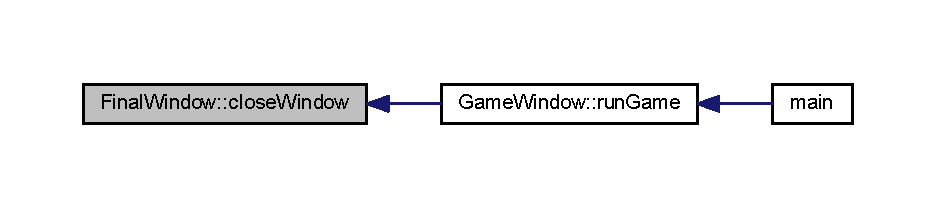
\includegraphics[width=350pt]{class_final_window_a3c5b82cb988e1f312c0f459959442e2b_icgraph}
\end{center}
\end{figure}
\mbox{\Hypertarget{class_final_window_a793b0fa86eac2eef3256d9d2f1f3711b}\label{class_final_window_a793b0fa86eac2eef3256d9d2f1f3711b}} 
\index{Final\+Window@{Final\+Window}!did\+Player\+Lose\+Game@{did\+Player\+Lose\+Game}}
\index{did\+Player\+Lose\+Game@{did\+Player\+Lose\+Game}!Final\+Window@{Final\+Window}}
\subsubsection{\texorpdfstring{did\+Player\+Lose\+Game()}{didPlayerLoseGame()}}
{\footnotesize\ttfamily bool Final\+Window\+::did\+Player\+Lose\+Game (\begin{DoxyParamCaption}{ }\end{DoxyParamCaption})}

Here is the caller graph for this function\+:\nopagebreak
\begin{figure}[H]
\begin{center}
\leavevmode
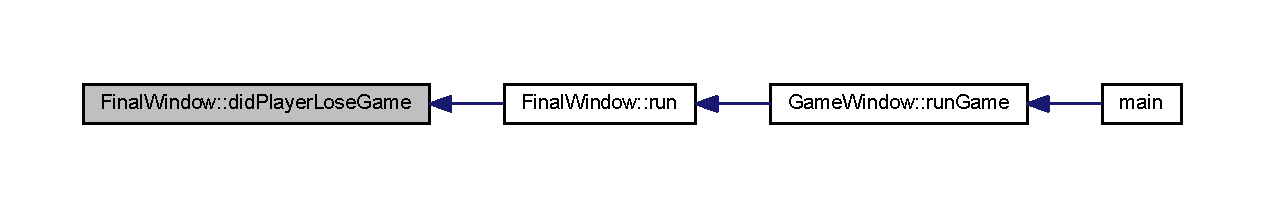
\includegraphics[width=350pt]{class_final_window_a793b0fa86eac2eef3256d9d2f1f3711b_icgraph}
\end{center}
\end{figure}
\mbox{\Hypertarget{class_final_window_aa719a7ffb084df7f00a72fdb0d843c38}\label{class_final_window_aa719a7ffb084df7f00a72fdb0d843c38}} 
\index{Final\+Window@{Final\+Window}!is\+Player\+Quitting\+Game@{is\+Player\+Quitting\+Game}}
\index{is\+Player\+Quitting\+Game@{is\+Player\+Quitting\+Game}!Final\+Window@{Final\+Window}}
\subsubsection{\texorpdfstring{is\+Player\+Quitting\+Game()}{isPlayerQuittingGame()}}
{\footnotesize\ttfamily bool Final\+Window\+::is\+Player\+Quitting\+Game (\begin{DoxyParamCaption}{ }\end{DoxyParamCaption})}



S\+T\+A\+T\+US Q\+U\+E\+RY F\+U\+N\+C\+T\+I\+O\+NS. 

\mbox{\Hypertarget{class_final_window_ad0ff2789d7ab310a4b70e393f602deff}\label{class_final_window_ad0ff2789d7ab310a4b70e393f602deff}} 
\index{Final\+Window@{Final\+Window}!run@{run}}
\index{run@{run}!Final\+Window@{Final\+Window}}
\subsubsection{\texorpdfstring{run()}{run()}}
{\footnotesize\ttfamily void Final\+Window\+::run (\begin{DoxyParamCaption}{ }\end{DoxyParamCaption})}

Here is the call graph for this function\+:\nopagebreak
\begin{figure}[H]
\begin{center}
\leavevmode
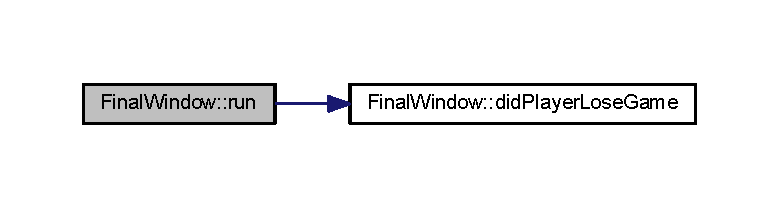
\includegraphics[width=350pt]{class_final_window_ad0ff2789d7ab310a4b70e393f602deff_cgraph}
\end{center}
\end{figure}
Here is the caller graph for this function\+:\nopagebreak
\begin{figure}[H]
\begin{center}
\leavevmode
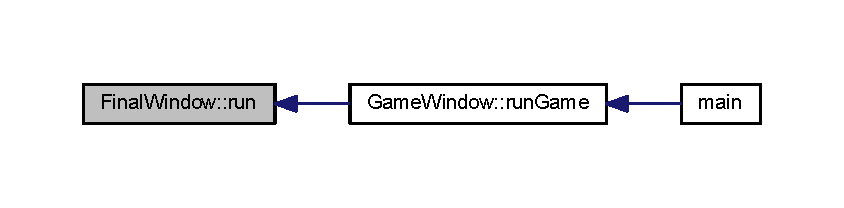
\includegraphics[width=350pt]{class_final_window_ad0ff2789d7ab310a4b70e393f602deff_icgraph}
\end{center}
\end{figure}
\mbox{\Hypertarget{class_final_window_a3ad8ebeede5375c9cd4732e794f076ac}\label{class_final_window_a3ad8ebeede5375c9cd4732e794f076ac}} 
\index{Final\+Window@{Final\+Window}!set\+P\+Layer\+Lost\+Game@{set\+P\+Layer\+Lost\+Game}}
\index{set\+P\+Layer\+Lost\+Game@{set\+P\+Layer\+Lost\+Game}!Final\+Window@{Final\+Window}}
\subsubsection{\texorpdfstring{set\+P\+Layer\+Lost\+Game()}{setPLayerLostGame()}}
{\footnotesize\ttfamily void Final\+Window\+::set\+P\+Layer\+Lost\+Game (\begin{DoxyParamCaption}\item[{bool}]{status }\end{DoxyParamCaption})}

Here is the caller graph for this function\+:\nopagebreak
\begin{figure}[H]
\begin{center}
\leavevmode
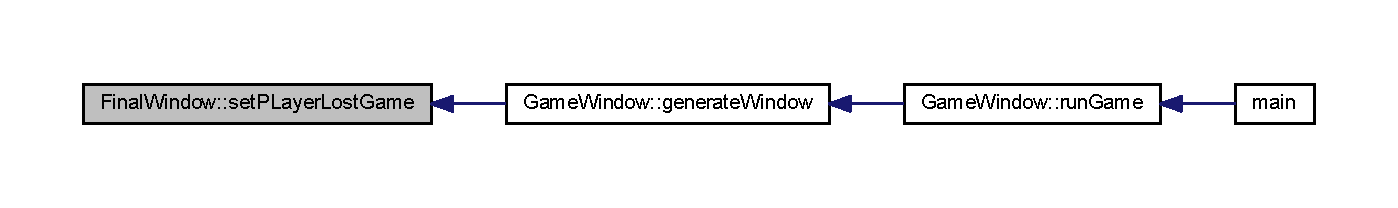
\includegraphics[width=350pt]{class_final_window_a3ad8ebeede5375c9cd4732e794f076ac_icgraph}
\end{center}
\end{figure}
\mbox{\Hypertarget{class_final_window_afd73d524fd2f10486d86a2e0057fcb54}\label{class_final_window_afd73d524fd2f10486d86a2e0057fcb54}} 
\index{Final\+Window@{Final\+Window}!set\+Quitting\+Game@{set\+Quitting\+Game}}
\index{set\+Quitting\+Game@{set\+Quitting\+Game}!Final\+Window@{Final\+Window}}
\subsubsection{\texorpdfstring{set\+Quitting\+Game()}{setQuittingGame()}}
{\footnotesize\ttfamily void Final\+Window\+::set\+Quitting\+Game (\begin{DoxyParamCaption}\item[{bool}]{decision }\end{DoxyParamCaption})}



S\+T\+A\+T\+US S\+E\+T\+T\+I\+NG F\+U\+N\+C\+T\+I\+N\+OS. 



The documentation for this class was generated from the following files\+:\begin{DoxyCompactItemize}
\item 
C\+:/\+Users/\+User/\+Documents/\+Software\+Dev2\+Project/\+Space\+Rider\+Project/\hyperlink{_final_window_8h}{Final\+Window.\+h}\item 
C\+:/\+Users/\+User/\+Documents/\+Software\+Dev2\+Project/\+Space\+Rider\+Project/\hyperlink{_final_window_8cpp}{Final\+Window.\+cpp}\end{DoxyCompactItemize}

\hypertarget{class_game_logic}{}\section{Game\+Logic Class Reference}
\label{class_game_logic}\index{Game\+Logic@{Game\+Logic}}
\subsection*{Public Member Functions}
\begin{DoxyCompactItemize}
\item 
\mbox{\Hypertarget{class_game_logic_a3bb909e55fc7c811aa0e3e6a92b881bb}\label{class_game_logic_a3bb909e55fc7c811aa0e3e6a92b881bb}} 
void {\bfseries player\+Update} (Direction dir)
\item 
\mbox{\Hypertarget{class_game_logic_a05dec53eb3c36cf1a669c973fa0b16ae}\label{class_game_logic_a05dec53eb3c36cf1a669c973fa0b16ae}} 
void {\bfseries create\+Player\+Bullet} ()
\item 
\mbox{\Hypertarget{class_game_logic_a2293e862afa9caa43ac1c21757b9c914}\label{class_game_logic_a2293e862afa9caa43ac1c21757b9c914}} 
void {\bfseries player\+Bullet\+Update} ()
\item 
\mbox{\Hypertarget{class_game_logic_abe02a85cda082eea7d0dc758d8fe3082}\label{class_game_logic_abe02a85cda082eea7d0dc758d8fe3082}} 
void {\bfseries update\+Player\+Bullet\+Logic} ()
\item 
\mbox{\Hypertarget{class_game_logic_aa0800f256ffc094ee5373d372c26c2ea}\label{class_game_logic_aa0800f256ffc094ee5373d372c26c2ea}} 
void {\bfseries check\+Bullet\+Scope} ()
\item 
\mbox{\Hypertarget{class_game_logic_ad88d3d16d008722d8a85449beb1ed589}\label{class_game_logic_ad88d3d16d008722d8a85449beb1ed589}} 
void {\bfseries create\+Enemy\+Logic\+Object} ()
\item 
\mbox{\Hypertarget{class_game_logic_a07cb8f8cb380fa2cd070aa30148a8ffd}\label{class_game_logic_a07cb8f8cb380fa2cd070aa30148a8ffd}} 
void {\bfseries update\+Enemy\+Logic} ()
\item 
\mbox{\Hypertarget{class_game_logic_a5c0dc59099b2e223c99fc4a4d51627f0}\label{class_game_logic_a5c0dc59099b2e223c99fc4a4d51627f0}} 
void {\bfseries check\+Enemy\+Scope} ()
\item 
\mbox{\Hypertarget{class_game_logic_a2ff25304164107a3f4549f108db95a23}\label{class_game_logic_a2ff25304164107a3f4549f108db95a23}} 
void {\bfseries check\+Collision} ()
\item 
\mbox{\Hypertarget{class_game_logic_ab2b56581a56239bb837e6eeea0a2991d}\label{class_game_logic_ab2b56581a56239bb837e6eeea0a2991d}} 
void {\bfseries create\+Satellites} ()
\item 
\mbox{\Hypertarget{class_game_logic_a7d3db89e4d9438756e01b203341dc7c0}\label{class_game_logic_a7d3db89e4d9438756e01b203341dc7c0}} 
void {\bfseries update\+Satellite\+Logic} ()
\item 
\mbox{\Hypertarget{class_game_logic_ab84e34d803932a798b76f1c3b8a4af83}\label{class_game_logic_ab84e34d803932a798b76f1c3b8a4af83}} 
void {\bfseries fire\+Satellite\+Bullet\+Logic} ()
\item 
\mbox{\Hypertarget{class_game_logic_a196e25b5a240f8383ce8eab971938fc6}\label{class_game_logic_a196e25b5a240f8383ce8eab971938fc6}} 
void {\bfseries check\+Satellite\+Bullet\+Scope} ()
\item 
\mbox{\Hypertarget{class_game_logic_a8463ab82ec024ace6457030f61430fc1}\label{class_game_logic_a8463ab82ec024ace6457030f61430fc1}} 
void {\bfseries set\+Player\+Bullet\+Type} (int type)
\item 
\mbox{\Hypertarget{class_game_logic_a933e3cb807803f40baa6dd8dffedd000}\label{class_game_logic_a933e3cb807803f40baa6dd8dffedd000}} 
int {\bfseries get\+Player\+Bullet\+Type} ()
\item 
\mbox{\Hypertarget{class_game_logic_a1737f742ce3b179ea3b5f579a97e7d47}\label{class_game_logic_a1737f742ce3b179ea3b5f579a97e7d47}} 
void {\bfseries update\+Player\+Life} ()
\item 
\mbox{\Hypertarget{class_game_logic_a42fb536e1740b6eeb4f80840250d685f}\label{class_game_logic_a42fb536e1740b6eeb4f80840250d685f}} 
int {\bfseries get\+Player\+Lives\+Remaining} ()
\item 
\mbox{\Hypertarget{class_game_logic_ae7b71b5f335308748366385de5c0d88a}\label{class_game_logic_ae7b71b5f335308748366385de5c0d88a}} 
void {\bfseries update\+Laser\+Logic} ()
\item 
\mbox{\Hypertarget{class_game_logic_ae19f7458c9a738410d9c54a393346e35}\label{class_game_logic_ae19f7458c9a738410d9c54a393346e35}} 
void {\bfseries create\+Laser\+Generator\+Logic} ()
\item 
\mbox{\Hypertarget{class_game_logic_ada1e9103a2d46866076c2d3b69c7eaff}\label{class_game_logic_ada1e9103a2d46866076c2d3b69c7eaff}} 
void {\bfseries check\+Laser\+Generator\+Scope} ()
\item 
\mbox{\Hypertarget{class_game_logic_ad9b8589c1559ac09ae5674c5c87be600}\label{class_game_logic_ad9b8589c1559ac09ae5674c5c87be600}} 
void {\bfseries create\+Asteroid} ()
\item 
\mbox{\Hypertarget{class_game_logic_aefda6025dfef46818697b11f4276dfa6}\label{class_game_logic_aefda6025dfef46818697b11f4276dfa6}} 
void {\bfseries update\+Asteroid\+Logic} ()
\item 
\mbox{\Hypertarget{class_game_logic_a35dcb163c584e620b876def784cbd7a4}\label{class_game_logic_a35dcb163c584e620b876def784cbd7a4}} 
void {\bfseries check\+Asteroid\+Bounds} ()
\item 
\mbox{\Hypertarget{class_game_logic_ae2bb92c22bea679a7467c592f253263b}\label{class_game_logic_ae2bb92c22bea679a7467c592f253263b}} 
void {\bfseries delete\+Out\+Of\+Scope\+Asteroids} (int index)
\item 
\mbox{\Hypertarget{class_game_logic_a612e0df42ffe7ab590ce5a87c94aa6c9}\label{class_game_logic_a612e0df42ffe7ab590ce5a87c94aa6c9}} 
bool {\bfseries check\+Player\+Life\+Dead} ()
\item 
\mbox{\Hypertarget{class_game_logic_a743d03f2c6dab3786addba9b2bc1e5dc}\label{class_game_logic_a743d03f2c6dab3786addba9b2bc1e5dc}} 
bool {\bfseries is\+Player\+Dead} ()
\item 
\mbox{\Hypertarget{class_game_logic_ad30541663e6b28e997646173fbdf344e}\label{class_game_logic_ad30541663e6b28e997646173fbdf344e}} 
\hyperlink{class_life_logic}{Life\+Logic} {\bfseries get\+Player\+Life\+Logic} ()
\item 
\mbox{\Hypertarget{class_game_logic_abe0e031ff3278ebb3c049b06f458e5b4}\label{class_game_logic_abe0e031ff3278ebb3c049b06f458e5b4}} 
vector$<$ \hyperlink{class_laser_generator_logic}{Laser\+Generator\+Logic} $>$ {\bfseries getlaser\+Generator\+Logic} ()
\item 
\mbox{\Hypertarget{class_game_logic_adc970904cd9d94e6e64b733863839ddf}\label{class_game_logic_adc970904cd9d94e6e64b733863839ddf}} 
void {\bfseries delete\+Laser\+Generator} ()
\item 
\mbox{\Hypertarget{class_game_logic_a52d34b124f0bf66dee3a144e4645e60c}\label{class_game_logic_a52d34b124f0bf66dee3a144e4645e60c}} 
vector$<$ \hyperlink{class_player_bullet}{Player\+Bullet} $>$ {\bfseries get\+Player\+Logic\+Bullets} ()
\item 
\mbox{\Hypertarget{class_game_logic_ae5629e5f0bf316435c6b4f40171755b9}\label{class_game_logic_ae5629e5f0bf316435c6b4f40171755b9}} 
void {\bfseries delete\+Player\+Bullet} (int index)
\item 
\mbox{\Hypertarget{class_game_logic_a7aeb038bd7a0feef3377745ae334011c}\label{class_game_logic_a7aeb038bd7a0feef3377745ae334011c}} 
\hyperlink{class_player_logic}{Player\+Logic} {\bfseries get\+Player\+Logic} ()
\item 
\mbox{\Hypertarget{class_game_logic_afa1fd0270df0970723f3aef06431e2d8}\label{class_game_logic_afa1fd0270df0970723f3aef06431e2d8}} 
vector$<$ \hyperlink{class_enemy_logic}{Enemy\+Logic} $>$ {\bfseries get\+Enemy\+Logic\+Vector} ()
\item 
\mbox{\Hypertarget{class_game_logic_a34fd5f74aec0365dff0631384740a45b}\label{class_game_logic_a34fd5f74aec0365dff0631384740a45b}} 
void {\bfseries delete\+Enemy\+Logic} (int index)
\item 
\mbox{\Hypertarget{class_game_logic_a48f8e18378ed00053d83da991fcad264}\label{class_game_logic_a48f8e18378ed00053d83da991fcad264}} 
void {\bfseries set\+Enemy\+Bounds} (bool is\+In\+Bounds, int index)
\item 
\mbox{\Hypertarget{class_game_logic_af355faaa66630a76a14ef0d7dc5adb54}\label{class_game_logic_af355faaa66630a76a14ef0d7dc5adb54}} 
void {\bfseries move\+Enemy\+To\+Center} (int index)
\item 
\mbox{\Hypertarget{class_game_logic_aa8b94076dcd3ad6419c50d0036af97d6}\label{class_game_logic_aa8b94076dcd3ad6419c50d0036af97d6}} 
void {\bfseries clear\+Enemy\+Bullet} (int index)
\item 
\mbox{\Hypertarget{class_game_logic_a1110f512d8382700d322c6f1895810ea}\label{class_game_logic_a1110f512d8382700d322c6f1895810ea}} 
vector$<$ \hyperlink{class_satellite_logic}{Satellite\+Logic} $>$ {\bfseries get\+Satellite\+Logic\+Vector} ()
\item 
\mbox{\Hypertarget{class_game_logic_a3954ee824ac3acc8753f61f97d41ce89}\label{class_game_logic_a3954ee824ac3acc8753f61f97d41ce89}} 
void {\bfseries delete\+Satellite\+Logic} (int index)
\item 
\mbox{\Hypertarget{class_game_logic_a230c5fb0084aa73c3b689c18a72b6adf}\label{class_game_logic_a230c5fb0084aa73c3b689c18a72b6adf}} 
vector$<$ \hyperlink{class_enemy_bullet_logic}{Enemy\+Bullet\+Logic} $>$ {\bfseries get\+Satelliet\+Bullet\+Logic\+Vector} ()
\item 
\mbox{\Hypertarget{class_game_logic_a4527756097ff2039fd91daad430e8598}\label{class_game_logic_a4527756097ff2039fd91daad430e8598}} 
void {\bfseries delete\+Satellite\+Bullet\+Logic} (int index)
\item 
\mbox{\Hypertarget{class_game_logic_a353d4a44a09214c0ed73aa3a26b2ce0d}\label{class_game_logic_a353d4a44a09214c0ed73aa3a26b2ce0d}} 
void {\bfseries update\+Satellite\+Bullets} (int index)
\item 
\mbox{\Hypertarget{class_game_logic_a084386ea39d66e3963ba248f7affabe0}\label{class_game_logic_a084386ea39d66e3963ba248f7affabe0}} 
vector$<$ \hyperlink{class_asteroid_logic}{Asteroid\+Logic} $>$ {\bfseries get\+Asteroid\+Logic\+Vector} ()
\item 
\mbox{\Hypertarget{class_game_logic_a594da37684d54d619214e8f96b80279c}\label{class_game_logic_a594da37684d54d619214e8f96b80279c}} 
void {\bfseries save\+Scoreto\+File} ()
\item 
\mbox{\Hypertarget{class_game_logic_a05ad3bbd5acd9f0b41d1f1d29cac8017}\label{class_game_logic_a05ad3bbd5acd9f0b41d1f1d29cac8017}} 
int {\bfseries get\+High\+Score} ()
\end{DoxyCompactItemize}


The documentation for this class was generated from the following files\+:\begin{DoxyCompactItemize}
\item 
C\+:/\+Users/\+William/\+Documents/\+E\+L\+E\+N3009/\+Space\+Rider\+Project/Game\+Logic.\+h\item 
C\+:/\+Users/\+William/\+Documents/\+E\+L\+E\+N3009/\+Space\+Rider\+Project/Game\+Logic.\+cpp\end{DoxyCompactItemize}

\hypertarget{class_game_presentation}{}\section{Game\+Presentation Class Reference}
\label{class_game_presentation}\index{Game\+Presentation@{Game\+Presentation}}


{\ttfamily \#include $<$Game\+Presentation.\+h$>$}



Collaboration diagram for Game\+Presentation\+:\nopagebreak
\begin{figure}[H]
\begin{center}
\leavevmode
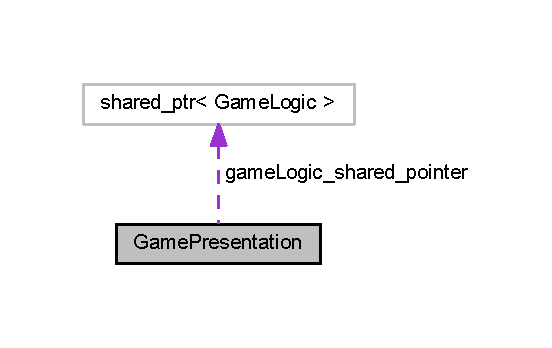
\includegraphics[width=265pt]{class_game_presentation__coll__graph}
\end{center}
\end{figure}
\subsection*{Public Member Functions}
\begin{DoxyCompactItemize}
\item 
\hyperlink{class_game_presentation_a14dbabbd4d03bd81522a95f235eefc4b}{Game\+Presentation} ()
\item 
void \hyperlink{class_game_presentation_ae2a317ddda3f666fdb1ca4f4c68f6b49}{render\+Sprite} (Render\+Window \&window)
\item 
void \hyperlink{class_game_presentation_a08abc97c6f65eda4ac7c54d55a9054b4}{up\+Date\+Player\+Position} ()
\item 
void \hyperlink{class_game_presentation_a027b38ee9bf11018b4db7494d2e145a0}{check\+Player\+Presentation\+Life\+Dead} ()
\item 
void \hyperlink{class_game_presentation_af0a19d50c4099e7a19426cdffa5ebb82}{up\+Date\+Player\+Bullet\+Presentation} ()
\item 
void \hyperlink{class_game_presentation_ac87927887e1afc5583036efb01ab35ca}{create\+Player\+Bullet\+Presentation} ()
\item 
void \hyperlink{class_game_presentation_a874688a19d648902d43751a198e2d9ab}{draw\+All\+Bullets} (Render\+Window \&window)
\item 
void \hyperlink{class_game_presentation_a313bd414a0cc712fccd919df4b794b8a}{delete\+Outof\+Scope\+Bullets} ()
\item 
void \hyperlink{class_game_presentation_a59645176840f6ddec2673b9d447334d5}{create\+Enemy\+Presentation\+Object} ()
\item 
void \hyperlink{class_game_presentation_a4ab96a6022c08f34aefa62f9a30c1cd8}{update\+Enemy\+Presentation} ()
\item 
void \hyperlink{class_game_presentation_af29e04c4a89f0a6d1ca9eab33da5ace5}{draw\+All\+Enemies} (Render\+Window \&window)
\item 
void \hyperlink{class_game_presentation_ae83bb9e0751f6077f2480a36dec36787}{delete\+Dead\+Enemies} ()
\item 
void \hyperlink{class_game_presentation_a921823ce61d5c9a0db91098c8f055d28}{create\+Satellite\+Presenetation} ()
\item 
void \hyperlink{class_game_presentation_a7a94467d53b62bd7a83035ea4fa386ac}{draw\+Satellites} (Render\+Window \&window)
\item 
void \hyperlink{class_game_presentation_acc8d59152c26b9dddc84081c5a4483f2}{delete\+Dead\+Enemy\+Bullets} ()
\item 
vector$<$ \hyperlink{class_satellite_presentation}{Satellite\+Presentation} $>$ \hyperlink{class_game_presentation_a8bb8847556bd4977479df73eec79b2eb}{get\+Satellite\+Presentation\+Vector} ()
\item 
void \hyperlink{class_game_presentation_a172770f122258cba73e1dbff88d27ea5}{create\+Satellite\+Bullet\+Presentation} ()
\item 
void \hyperlink{class_game_presentation_a6ee175034a6d067f2755c75c753f07a0}{draw\+Satellite\+Bullets} (Render\+Window \&window)
\item 
void \hyperlink{class_game_presentation_a5a329f0403011b464c26218eeff38606}{set\+Player\+Life\+Count} ()
\item 
void \hyperlink{class_game_presentation_ac20ace0966aacedc817bdafd6eb6f1ba}{create\+Laser\+Generator} ()
\item 
void \hyperlink{class_game_presentation_a8c0ec310f4105564f11d1b48779e3941}{draw\+Laser\+Generator} (Render\+Window \&window)
\item 
void \hyperlink{class_game_presentation_aa6d8e5e91de557ac2c39bb51e032f14f}{update\+Laser\+Generator\+Presentation} ()
\item 
void \hyperlink{class_game_presentation_aebd299a3aa0c8e7a06d63f5cbc808c7d}{delete\+Laser\+Generator} ()
\item 
void \hyperlink{class_game_presentation_a4c3e9bf3b8866eaff58c5eb8c83f3245}{create\+Asteroid\+Presentation} ()
\item 
void \hyperlink{class_game_presentation_a669fe49aef6332f78a23802cafa6681c}{update\+Asteroid\+Presentation} ()
\item 
void \hyperlink{class_game_presentation_adbeb1c114932cdab67120bd6fe6a5da5}{draw\+Asteroid} (Render\+Window \&window)
\item 
void \hyperlink{class_game_presentation_acd19622d7ee0ae8b898f5805ae94f2b4}{delete\+Outof\+Scope\+Asteroids\+Presentation} ()
\item 
void \hyperlink{class_game_presentation_ab2cf74842583bf5b63e5973fb8b657be}{update\+Score\+Presentation} ()
\item 
void \hyperlink{class_game_presentation_a38bab53e3d75b244e14ed2d7c2710fa0}{draw\+Score\+Presentation} (Render\+Window \&window)
\item 
int \hyperlink{class_game_presentation_ab09fbeaf4a3dfd753f1bce5cdd78969e}{get\+Enemies\+Killed} ()
\item 
vector$<$ \hyperlink{class_enemy_presentation}{Enemy\+Presentation} $>$ \hyperlink{class_game_presentation_a903a8e09c19324b2380b5073abd570f0}{get\+Enemy\+Presentation\+Vector} ()
\item 
vector$<$ \hyperlink{class_laser_generator_presentation}{Laser\+Generator\+Presentation} $>$ \hyperlink{class_game_presentation_a6da88c7baf912bccf09f274b6a5ae7b6}{get\+Laser\+Generator\+Presentation} ()
\item 
vector$<$ \hyperlink{class_asteroid_presentation}{Asteroid\+Presentation} $>$ \hyperlink{class_game_presentation_a28a7d4fb65413d6a10b960721aaca0d2}{get\+Asteroid\+Presentation\+Vector} ()
\end{DoxyCompactItemize}
\subsection*{Public Attributes}
\begin{DoxyCompactItemize}
\item 
shared\+\_\+ptr$<$ \hyperlink{class_game_logic}{Game\+Logic} $>$ \hyperlink{class_game_presentation_a2f149f73bdd87ded8a6d66ecc427352f}{game\+Logic\+\_\+shared\+\_\+pointer}
\end{DoxyCompactItemize}


\subsection{Constructor \& Destructor Documentation}
\mbox{\Hypertarget{class_game_presentation_a14dbabbd4d03bd81522a95f235eefc4b}\label{class_game_presentation_a14dbabbd4d03bd81522a95f235eefc4b}} 
\index{Game\+Presentation@{Game\+Presentation}!Game\+Presentation@{Game\+Presentation}}
\index{Game\+Presentation@{Game\+Presentation}!Game\+Presentation@{Game\+Presentation}}
\subsubsection{\texorpdfstring{Game\+Presentation()}{GamePresentation()}}
{\footnotesize\ttfamily Game\+Presentation\+::\+Game\+Presentation (\begin{DoxyParamCaption}{ }\end{DoxyParamCaption})}



\subsection{Member Function Documentation}
\mbox{\Hypertarget{class_game_presentation_a027b38ee9bf11018b4db7494d2e145a0}\label{class_game_presentation_a027b38ee9bf11018b4db7494d2e145a0}} 
\index{Game\+Presentation@{Game\+Presentation}!check\+Player\+Presentation\+Life\+Dead@{check\+Player\+Presentation\+Life\+Dead}}
\index{check\+Player\+Presentation\+Life\+Dead@{check\+Player\+Presentation\+Life\+Dead}!Game\+Presentation@{Game\+Presentation}}
\subsubsection{\texorpdfstring{check\+Player\+Presentation\+Life\+Dead()}{checkPlayerPresentationLifeDead()}}
{\footnotesize\ttfamily void Game\+Presentation\+::check\+Player\+Presentation\+Life\+Dead (\begin{DoxyParamCaption}{ }\end{DoxyParamCaption})}

Here is the call graph for this function\+:\nopagebreak
\begin{figure}[H]
\begin{center}
\leavevmode
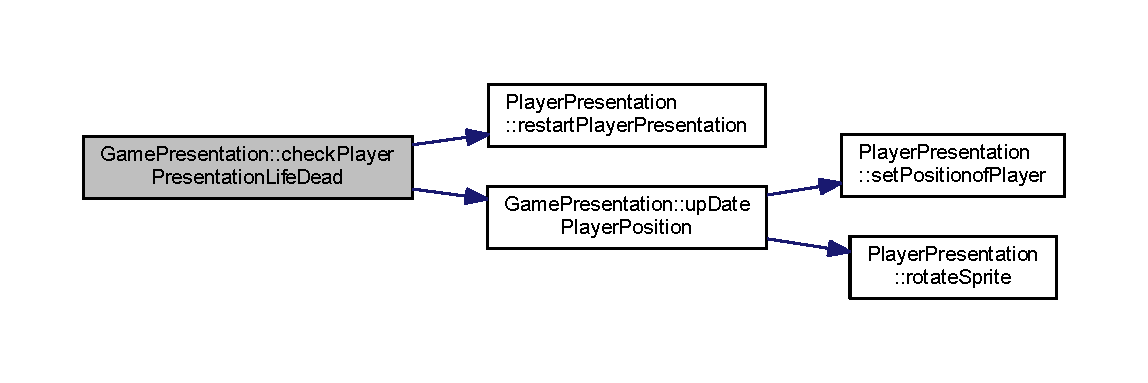
\includegraphics[width=350pt]{class_game_presentation_a027b38ee9bf11018b4db7494d2e145a0_cgraph}
\end{center}
\end{figure}
Here is the caller graph for this function\+:\nopagebreak
\begin{figure}[H]
\begin{center}
\leavevmode
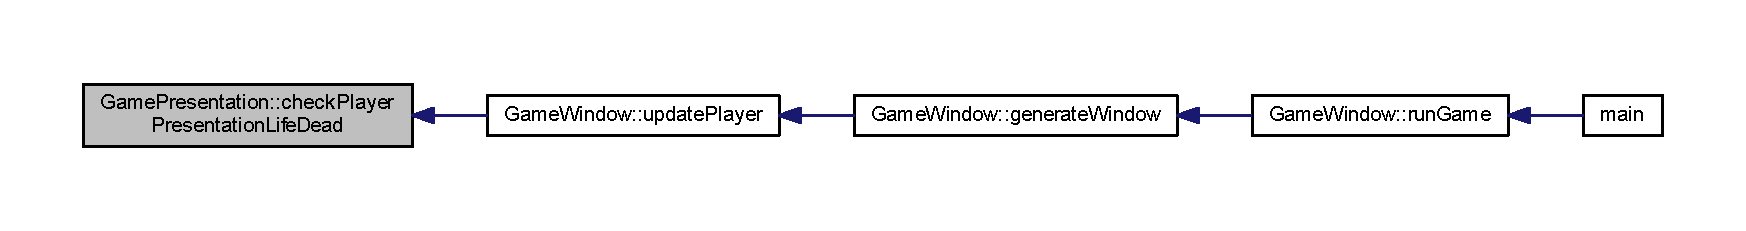
\includegraphics[width=350pt]{class_game_presentation_a027b38ee9bf11018b4db7494d2e145a0_icgraph}
\end{center}
\end{figure}
\mbox{\Hypertarget{class_game_presentation_a4c3e9bf3b8866eaff58c5eb8c83f3245}\label{class_game_presentation_a4c3e9bf3b8866eaff58c5eb8c83f3245}} 
\index{Game\+Presentation@{Game\+Presentation}!create\+Asteroid\+Presentation@{create\+Asteroid\+Presentation}}
\index{create\+Asteroid\+Presentation@{create\+Asteroid\+Presentation}!Game\+Presentation@{Game\+Presentation}}
\subsubsection{\texorpdfstring{create\+Asteroid\+Presentation()}{createAsteroidPresentation()}}
{\footnotesize\ttfamily void Game\+Presentation\+::create\+Asteroid\+Presentation (\begin{DoxyParamCaption}{ }\end{DoxyParamCaption})}

Here is the caller graph for this function\+:\nopagebreak
\begin{figure}[H]
\begin{center}
\leavevmode
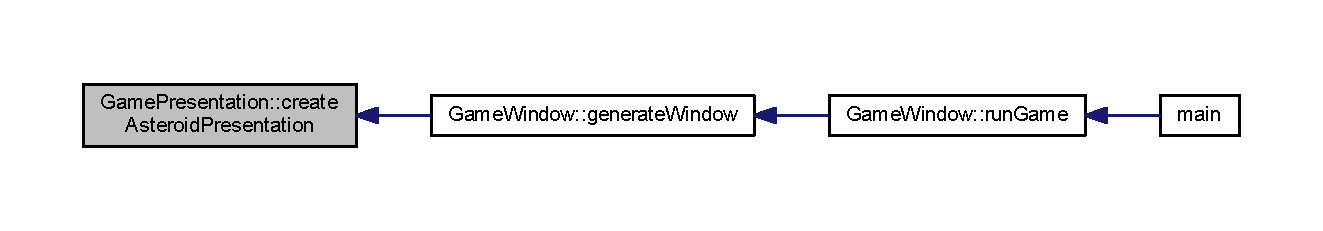
\includegraphics[width=350pt]{class_game_presentation_a4c3e9bf3b8866eaff58c5eb8c83f3245_icgraph}
\end{center}
\end{figure}
\mbox{\Hypertarget{class_game_presentation_a59645176840f6ddec2673b9d447334d5}\label{class_game_presentation_a59645176840f6ddec2673b9d447334d5}} 
\index{Game\+Presentation@{Game\+Presentation}!create\+Enemy\+Presentation\+Object@{create\+Enemy\+Presentation\+Object}}
\index{create\+Enemy\+Presentation\+Object@{create\+Enemy\+Presentation\+Object}!Game\+Presentation@{Game\+Presentation}}
\subsubsection{\texorpdfstring{create\+Enemy\+Presentation\+Object()}{createEnemyPresentationObject()}}
{\footnotesize\ttfamily void Game\+Presentation\+::create\+Enemy\+Presentation\+Object (\begin{DoxyParamCaption}{ }\end{DoxyParamCaption})}

Here is the caller graph for this function\+:\nopagebreak
\begin{figure}[H]
\begin{center}
\leavevmode
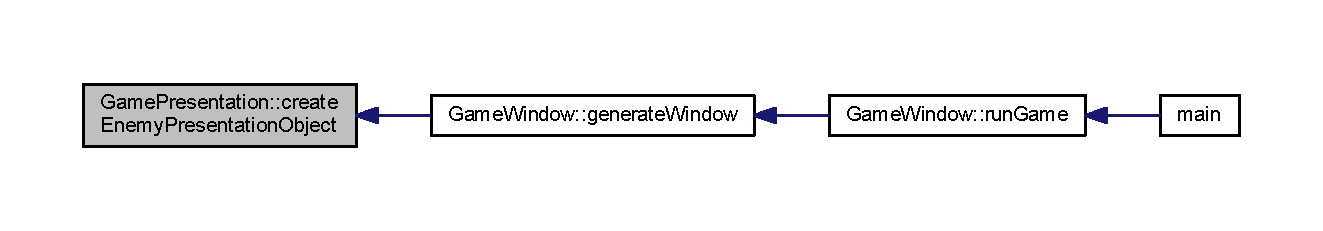
\includegraphics[width=350pt]{class_game_presentation_a59645176840f6ddec2673b9d447334d5_icgraph}
\end{center}
\end{figure}
\mbox{\Hypertarget{class_game_presentation_ac20ace0966aacedc817bdafd6eb6f1ba}\label{class_game_presentation_ac20ace0966aacedc817bdafd6eb6f1ba}} 
\index{Game\+Presentation@{Game\+Presentation}!create\+Laser\+Generator@{create\+Laser\+Generator}}
\index{create\+Laser\+Generator@{create\+Laser\+Generator}!Game\+Presentation@{Game\+Presentation}}
\subsubsection{\texorpdfstring{create\+Laser\+Generator()}{createLaserGenerator()}}
{\footnotesize\ttfamily void Game\+Presentation\+::create\+Laser\+Generator (\begin{DoxyParamCaption}{ }\end{DoxyParamCaption})}

Here is the caller graph for this function\+:\nopagebreak
\begin{figure}[H]
\begin{center}
\leavevmode
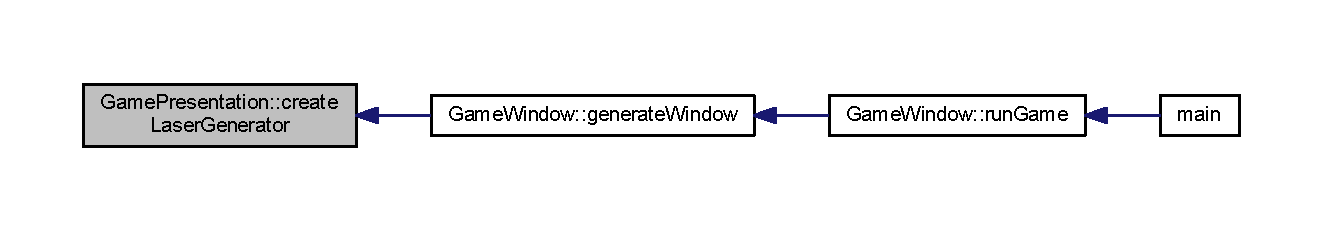
\includegraphics[width=350pt]{class_game_presentation_ac20ace0966aacedc817bdafd6eb6f1ba_icgraph}
\end{center}
\end{figure}
\mbox{\Hypertarget{class_game_presentation_ac87927887e1afc5583036efb01ab35ca}\label{class_game_presentation_ac87927887e1afc5583036efb01ab35ca}} 
\index{Game\+Presentation@{Game\+Presentation}!create\+Player\+Bullet\+Presentation@{create\+Player\+Bullet\+Presentation}}
\index{create\+Player\+Bullet\+Presentation@{create\+Player\+Bullet\+Presentation}!Game\+Presentation@{Game\+Presentation}}
\subsubsection{\texorpdfstring{create\+Player\+Bullet\+Presentation()}{createPlayerBulletPresentation()}}
{\footnotesize\ttfamily void Game\+Presentation\+::create\+Player\+Bullet\+Presentation (\begin{DoxyParamCaption}{ }\end{DoxyParamCaption})}

Here is the caller graph for this function\+:\nopagebreak
\begin{figure}[H]
\begin{center}
\leavevmode
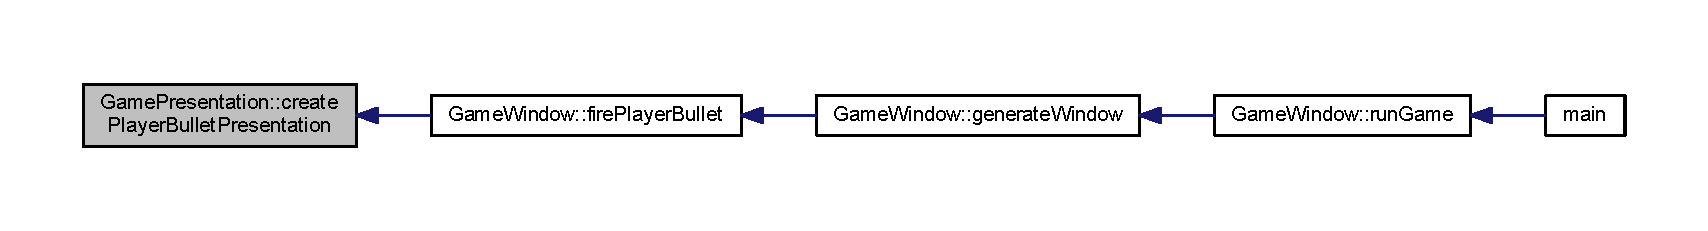
\includegraphics[width=350pt]{class_game_presentation_ac87927887e1afc5583036efb01ab35ca_icgraph}
\end{center}
\end{figure}
\mbox{\Hypertarget{class_game_presentation_a172770f122258cba73e1dbff88d27ea5}\label{class_game_presentation_a172770f122258cba73e1dbff88d27ea5}} 
\index{Game\+Presentation@{Game\+Presentation}!create\+Satellite\+Bullet\+Presentation@{create\+Satellite\+Bullet\+Presentation}}
\index{create\+Satellite\+Bullet\+Presentation@{create\+Satellite\+Bullet\+Presentation}!Game\+Presentation@{Game\+Presentation}}
\subsubsection{\texorpdfstring{create\+Satellite\+Bullet\+Presentation()}{createSatelliteBulletPresentation()}}
{\footnotesize\ttfamily void Game\+Presentation\+::create\+Satellite\+Bullet\+Presentation (\begin{DoxyParamCaption}{ }\end{DoxyParamCaption})}

Here is the caller graph for this function\+:\nopagebreak
\begin{figure}[H]
\begin{center}
\leavevmode
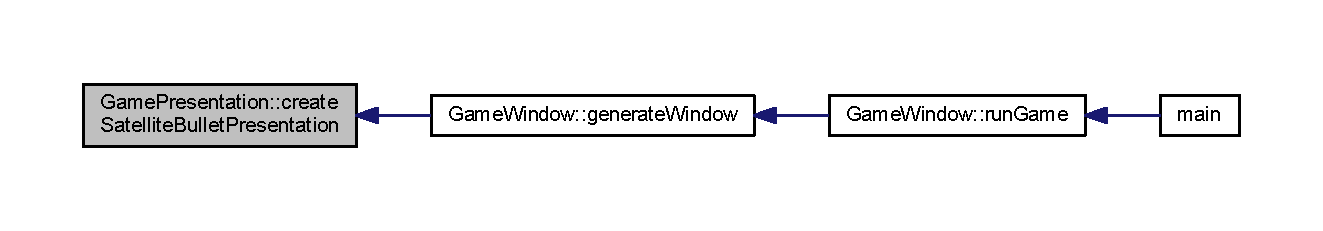
\includegraphics[width=350pt]{class_game_presentation_a172770f122258cba73e1dbff88d27ea5_icgraph}
\end{center}
\end{figure}
\mbox{\Hypertarget{class_game_presentation_a921823ce61d5c9a0db91098c8f055d28}\label{class_game_presentation_a921823ce61d5c9a0db91098c8f055d28}} 
\index{Game\+Presentation@{Game\+Presentation}!create\+Satellite\+Presenetation@{create\+Satellite\+Presenetation}}
\index{create\+Satellite\+Presenetation@{create\+Satellite\+Presenetation}!Game\+Presentation@{Game\+Presentation}}
\subsubsection{\texorpdfstring{create\+Satellite\+Presenetation()}{createSatellitePresenetation()}}
{\footnotesize\ttfamily void Game\+Presentation\+::create\+Satellite\+Presenetation (\begin{DoxyParamCaption}{ }\end{DoxyParamCaption})}

Here is the caller graph for this function\+:\nopagebreak
\begin{figure}[H]
\begin{center}
\leavevmode
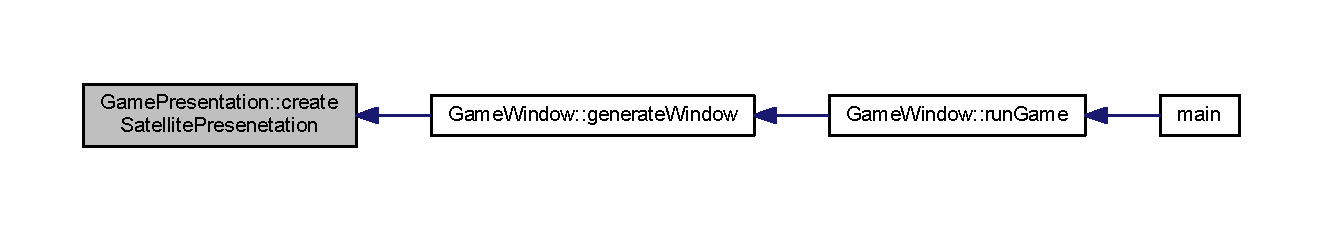
\includegraphics[width=350pt]{class_game_presentation_a921823ce61d5c9a0db91098c8f055d28_icgraph}
\end{center}
\end{figure}
\mbox{\Hypertarget{class_game_presentation_ae83bb9e0751f6077f2480a36dec36787}\label{class_game_presentation_ae83bb9e0751f6077f2480a36dec36787}} 
\index{Game\+Presentation@{Game\+Presentation}!delete\+Dead\+Enemies@{delete\+Dead\+Enemies}}
\index{delete\+Dead\+Enemies@{delete\+Dead\+Enemies}!Game\+Presentation@{Game\+Presentation}}
\subsubsection{\texorpdfstring{delete\+Dead\+Enemies()}{deleteDeadEnemies()}}
{\footnotesize\ttfamily void Game\+Presentation\+::delete\+Dead\+Enemies (\begin{DoxyParamCaption}{ }\end{DoxyParamCaption})}

Here is the caller graph for this function\+:\nopagebreak
\begin{figure}[H]
\begin{center}
\leavevmode
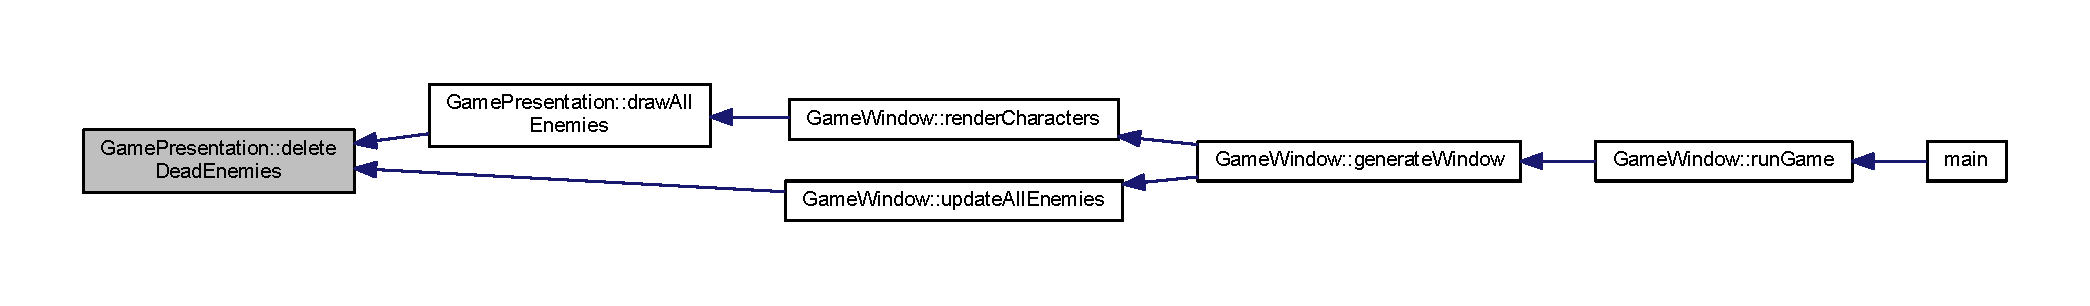
\includegraphics[width=350pt]{class_game_presentation_ae83bb9e0751f6077f2480a36dec36787_icgraph}
\end{center}
\end{figure}
\mbox{\Hypertarget{class_game_presentation_acc8d59152c26b9dddc84081c5a4483f2}\label{class_game_presentation_acc8d59152c26b9dddc84081c5a4483f2}} 
\index{Game\+Presentation@{Game\+Presentation}!delete\+Dead\+Enemy\+Bullets@{delete\+Dead\+Enemy\+Bullets}}
\index{delete\+Dead\+Enemy\+Bullets@{delete\+Dead\+Enemy\+Bullets}!Game\+Presentation@{Game\+Presentation}}
\subsubsection{\texorpdfstring{delete\+Dead\+Enemy\+Bullets()}{deleteDeadEnemyBullets()}}
{\footnotesize\ttfamily void Game\+Presentation\+::delete\+Dead\+Enemy\+Bullets (\begin{DoxyParamCaption}{ }\end{DoxyParamCaption})}

Here is the caller graph for this function\+:\nopagebreak
\begin{figure}[H]
\begin{center}
\leavevmode
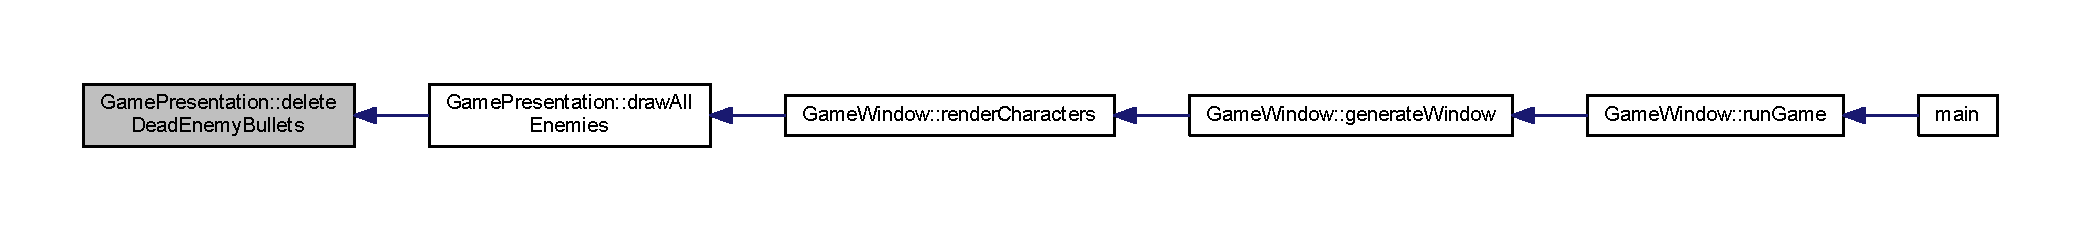
\includegraphics[width=350pt]{class_game_presentation_acc8d59152c26b9dddc84081c5a4483f2_icgraph}
\end{center}
\end{figure}
\mbox{\Hypertarget{class_game_presentation_aebd299a3aa0c8e7a06d63f5cbc808c7d}\label{class_game_presentation_aebd299a3aa0c8e7a06d63f5cbc808c7d}} 
\index{Game\+Presentation@{Game\+Presentation}!delete\+Laser\+Generator@{delete\+Laser\+Generator}}
\index{delete\+Laser\+Generator@{delete\+Laser\+Generator}!Game\+Presentation@{Game\+Presentation}}
\subsubsection{\texorpdfstring{delete\+Laser\+Generator()}{deleteLaserGenerator()}}
{\footnotesize\ttfamily void Game\+Presentation\+::delete\+Laser\+Generator (\begin{DoxyParamCaption}{ }\end{DoxyParamCaption})}

Here is the caller graph for this function\+:\nopagebreak
\begin{figure}[H]
\begin{center}
\leavevmode
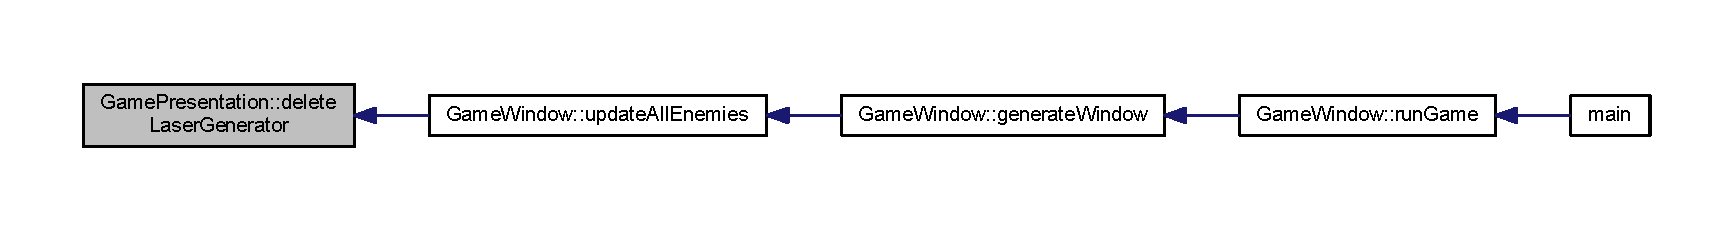
\includegraphics[width=350pt]{class_game_presentation_aebd299a3aa0c8e7a06d63f5cbc808c7d_icgraph}
\end{center}
\end{figure}
\mbox{\Hypertarget{class_game_presentation_acd19622d7ee0ae8b898f5805ae94f2b4}\label{class_game_presentation_acd19622d7ee0ae8b898f5805ae94f2b4}} 
\index{Game\+Presentation@{Game\+Presentation}!delete\+Outof\+Scope\+Asteroids\+Presentation@{delete\+Outof\+Scope\+Asteroids\+Presentation}}
\index{delete\+Outof\+Scope\+Asteroids\+Presentation@{delete\+Outof\+Scope\+Asteroids\+Presentation}!Game\+Presentation@{Game\+Presentation}}
\subsubsection{\texorpdfstring{delete\+Outof\+Scope\+Asteroids\+Presentation()}{deleteOutofScopeAsteroidsPresentation()}}
{\footnotesize\ttfamily void Game\+Presentation\+::delete\+Outof\+Scope\+Asteroids\+Presentation (\begin{DoxyParamCaption}{ }\end{DoxyParamCaption})}

Here is the caller graph for this function\+:\nopagebreak
\begin{figure}[H]
\begin{center}
\leavevmode
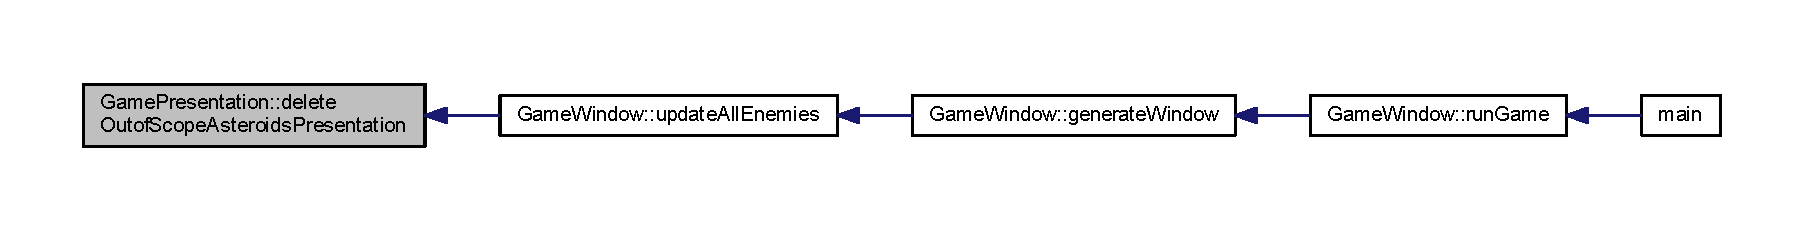
\includegraphics[width=350pt]{class_game_presentation_acd19622d7ee0ae8b898f5805ae94f2b4_icgraph}
\end{center}
\end{figure}
\mbox{\Hypertarget{class_game_presentation_a313bd414a0cc712fccd919df4b794b8a}\label{class_game_presentation_a313bd414a0cc712fccd919df4b794b8a}} 
\index{Game\+Presentation@{Game\+Presentation}!delete\+Outof\+Scope\+Bullets@{delete\+Outof\+Scope\+Bullets}}
\index{delete\+Outof\+Scope\+Bullets@{delete\+Outof\+Scope\+Bullets}!Game\+Presentation@{Game\+Presentation}}
\subsubsection{\texorpdfstring{delete\+Outof\+Scope\+Bullets()}{deleteOutofScopeBullets()}}
{\footnotesize\ttfamily void Game\+Presentation\+::delete\+Outof\+Scope\+Bullets (\begin{DoxyParamCaption}{ }\end{DoxyParamCaption})}

Here is the caller graph for this function\+:\nopagebreak
\begin{figure}[H]
\begin{center}
\leavevmode
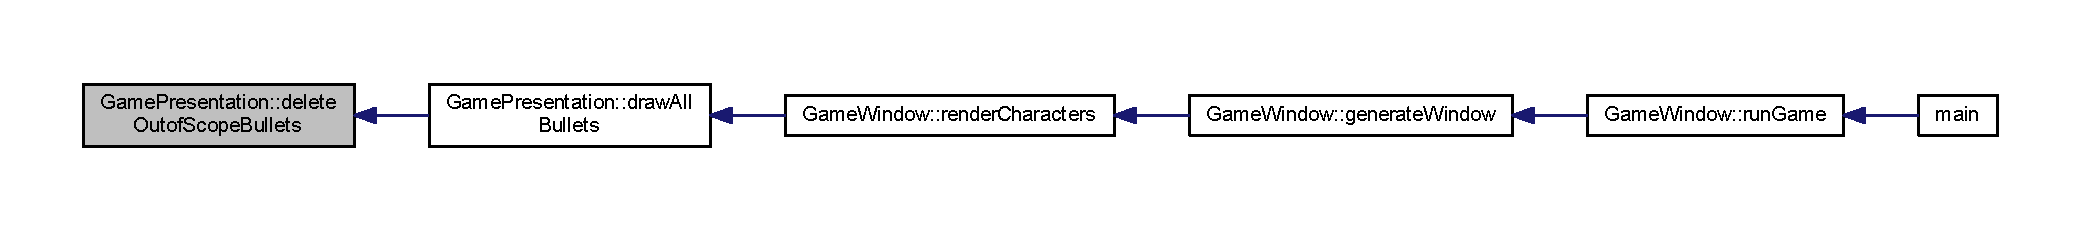
\includegraphics[width=350pt]{class_game_presentation_a313bd414a0cc712fccd919df4b794b8a_icgraph}
\end{center}
\end{figure}
\mbox{\Hypertarget{class_game_presentation_a874688a19d648902d43751a198e2d9ab}\label{class_game_presentation_a874688a19d648902d43751a198e2d9ab}} 
\index{Game\+Presentation@{Game\+Presentation}!draw\+All\+Bullets@{draw\+All\+Bullets}}
\index{draw\+All\+Bullets@{draw\+All\+Bullets}!Game\+Presentation@{Game\+Presentation}}
\subsubsection{\texorpdfstring{draw\+All\+Bullets()}{drawAllBullets()}}
{\footnotesize\ttfamily void Game\+Presentation\+::draw\+All\+Bullets (\begin{DoxyParamCaption}\item[{Render\+Window \&}]{window }\end{DoxyParamCaption})}

Here is the call graph for this function\+:\nopagebreak
\begin{figure}[H]
\begin{center}
\leavevmode
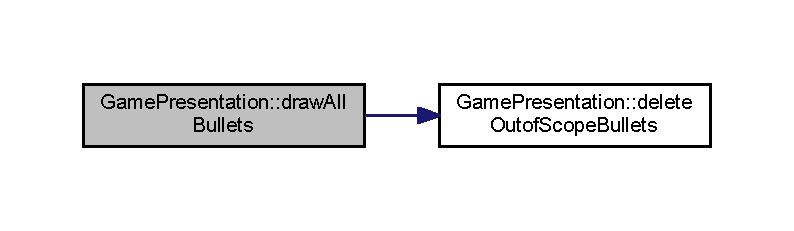
\includegraphics[width=350pt]{class_game_presentation_a874688a19d648902d43751a198e2d9ab_cgraph}
\end{center}
\end{figure}
Here is the caller graph for this function\+:\nopagebreak
\begin{figure}[H]
\begin{center}
\leavevmode
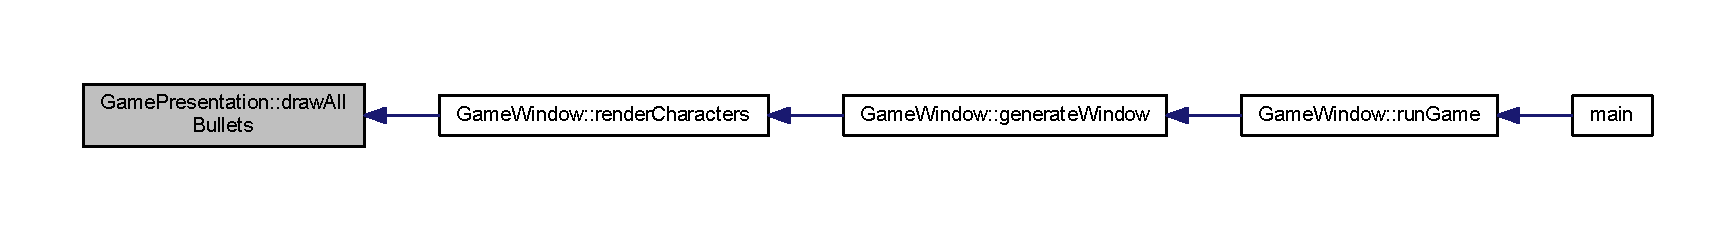
\includegraphics[width=350pt]{class_game_presentation_a874688a19d648902d43751a198e2d9ab_icgraph}
\end{center}
\end{figure}
\mbox{\Hypertarget{class_game_presentation_af29e04c4a89f0a6d1ca9eab33da5ace5}\label{class_game_presentation_af29e04c4a89f0a6d1ca9eab33da5ace5}} 
\index{Game\+Presentation@{Game\+Presentation}!draw\+All\+Enemies@{draw\+All\+Enemies}}
\index{draw\+All\+Enemies@{draw\+All\+Enemies}!Game\+Presentation@{Game\+Presentation}}
\subsubsection{\texorpdfstring{draw\+All\+Enemies()}{drawAllEnemies()}}
{\footnotesize\ttfamily void Game\+Presentation\+::draw\+All\+Enemies (\begin{DoxyParamCaption}\item[{Render\+Window \&}]{window }\end{DoxyParamCaption})}

Here is the call graph for this function\+:\nopagebreak
\begin{figure}[H]
\begin{center}
\leavevmode
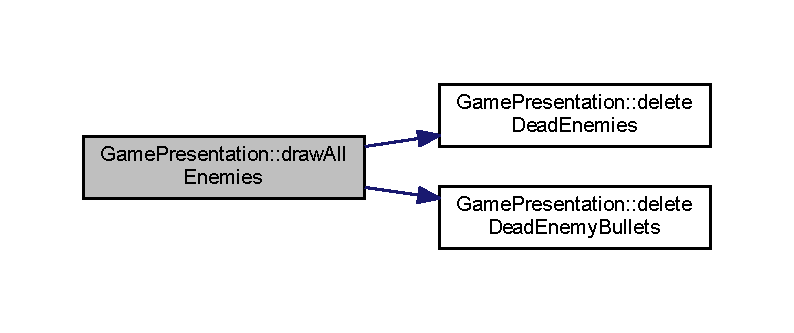
\includegraphics[width=350pt]{class_game_presentation_af29e04c4a89f0a6d1ca9eab33da5ace5_cgraph}
\end{center}
\end{figure}
Here is the caller graph for this function\+:\nopagebreak
\begin{figure}[H]
\begin{center}
\leavevmode
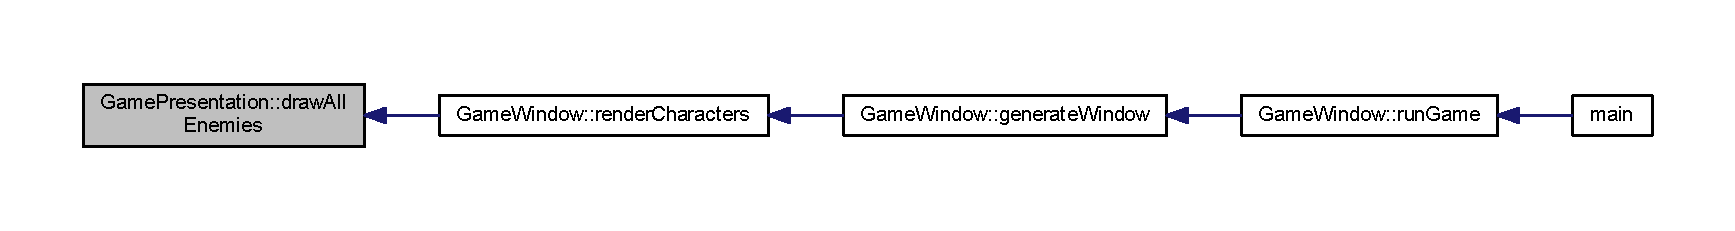
\includegraphics[width=350pt]{class_game_presentation_af29e04c4a89f0a6d1ca9eab33da5ace5_icgraph}
\end{center}
\end{figure}
\mbox{\Hypertarget{class_game_presentation_adbeb1c114932cdab67120bd6fe6a5da5}\label{class_game_presentation_adbeb1c114932cdab67120bd6fe6a5da5}} 
\index{Game\+Presentation@{Game\+Presentation}!draw\+Asteroid@{draw\+Asteroid}}
\index{draw\+Asteroid@{draw\+Asteroid}!Game\+Presentation@{Game\+Presentation}}
\subsubsection{\texorpdfstring{draw\+Asteroid()}{drawAsteroid()}}
{\footnotesize\ttfamily void Game\+Presentation\+::draw\+Asteroid (\begin{DoxyParamCaption}\item[{Render\+Window \&}]{window }\end{DoxyParamCaption})}

Here is the caller graph for this function\+:\nopagebreak
\begin{figure}[H]
\begin{center}
\leavevmode
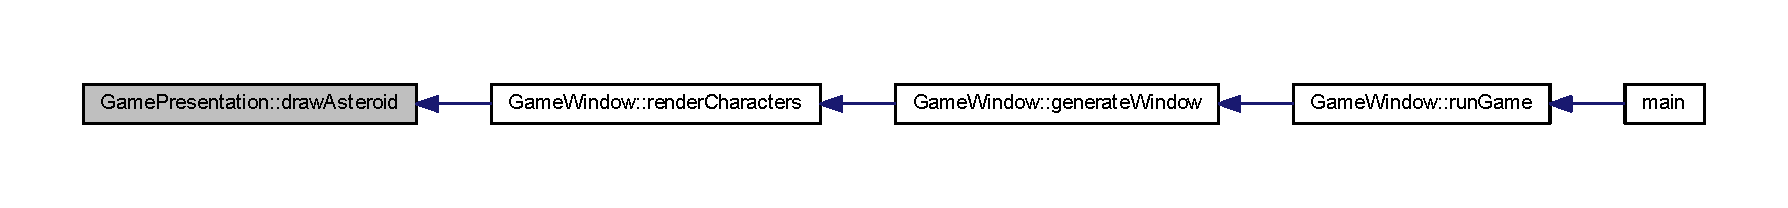
\includegraphics[width=350pt]{class_game_presentation_adbeb1c114932cdab67120bd6fe6a5da5_icgraph}
\end{center}
\end{figure}
\mbox{\Hypertarget{class_game_presentation_a8c0ec310f4105564f11d1b48779e3941}\label{class_game_presentation_a8c0ec310f4105564f11d1b48779e3941}} 
\index{Game\+Presentation@{Game\+Presentation}!draw\+Laser\+Generator@{draw\+Laser\+Generator}}
\index{draw\+Laser\+Generator@{draw\+Laser\+Generator}!Game\+Presentation@{Game\+Presentation}}
\subsubsection{\texorpdfstring{draw\+Laser\+Generator()}{drawLaserGenerator()}}
{\footnotesize\ttfamily void Game\+Presentation\+::draw\+Laser\+Generator (\begin{DoxyParamCaption}\item[{Render\+Window \&}]{window }\end{DoxyParamCaption})}

Here is the caller graph for this function\+:\nopagebreak
\begin{figure}[H]
\begin{center}
\leavevmode
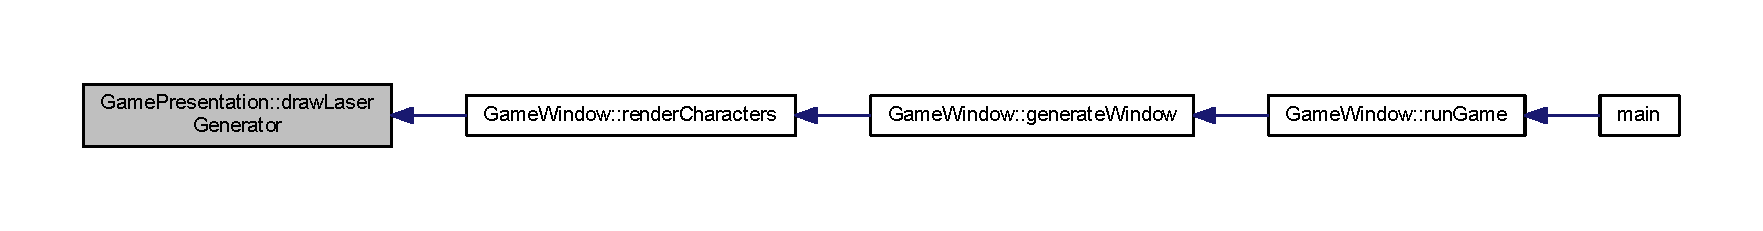
\includegraphics[width=350pt]{class_game_presentation_a8c0ec310f4105564f11d1b48779e3941_icgraph}
\end{center}
\end{figure}
\mbox{\Hypertarget{class_game_presentation_a6ee175034a6d067f2755c75c753f07a0}\label{class_game_presentation_a6ee175034a6d067f2755c75c753f07a0}} 
\index{Game\+Presentation@{Game\+Presentation}!draw\+Satellite\+Bullets@{draw\+Satellite\+Bullets}}
\index{draw\+Satellite\+Bullets@{draw\+Satellite\+Bullets}!Game\+Presentation@{Game\+Presentation}}
\subsubsection{\texorpdfstring{draw\+Satellite\+Bullets()}{drawSatelliteBullets()}}
{\footnotesize\ttfamily void Game\+Presentation\+::draw\+Satellite\+Bullets (\begin{DoxyParamCaption}\item[{Render\+Window \&}]{window }\end{DoxyParamCaption})}

Here is the caller graph for this function\+:\nopagebreak
\begin{figure}[H]
\begin{center}
\leavevmode
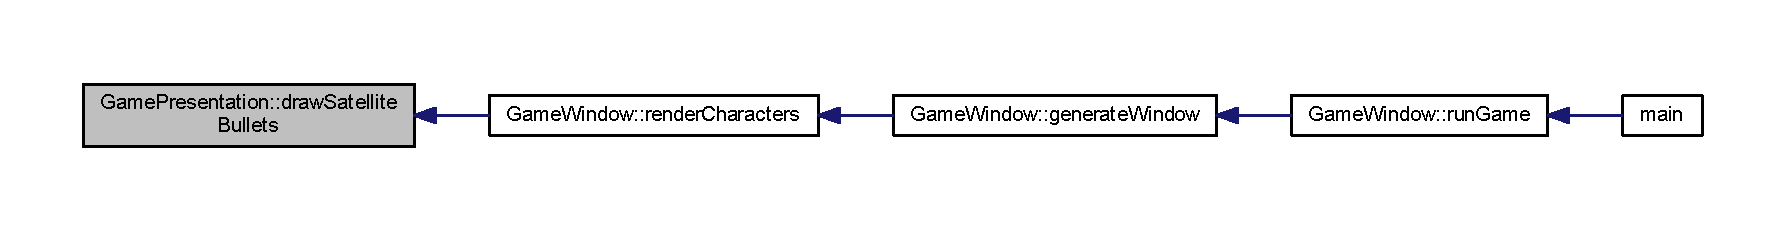
\includegraphics[width=350pt]{class_game_presentation_a6ee175034a6d067f2755c75c753f07a0_icgraph}
\end{center}
\end{figure}
\mbox{\Hypertarget{class_game_presentation_a7a94467d53b62bd7a83035ea4fa386ac}\label{class_game_presentation_a7a94467d53b62bd7a83035ea4fa386ac}} 
\index{Game\+Presentation@{Game\+Presentation}!draw\+Satellites@{draw\+Satellites}}
\index{draw\+Satellites@{draw\+Satellites}!Game\+Presentation@{Game\+Presentation}}
\subsubsection{\texorpdfstring{draw\+Satellites()}{drawSatellites()}}
{\footnotesize\ttfamily void Game\+Presentation\+::draw\+Satellites (\begin{DoxyParamCaption}\item[{Render\+Window \&}]{window }\end{DoxyParamCaption})}

Here is the caller graph for this function\+:\nopagebreak
\begin{figure}[H]
\begin{center}
\leavevmode
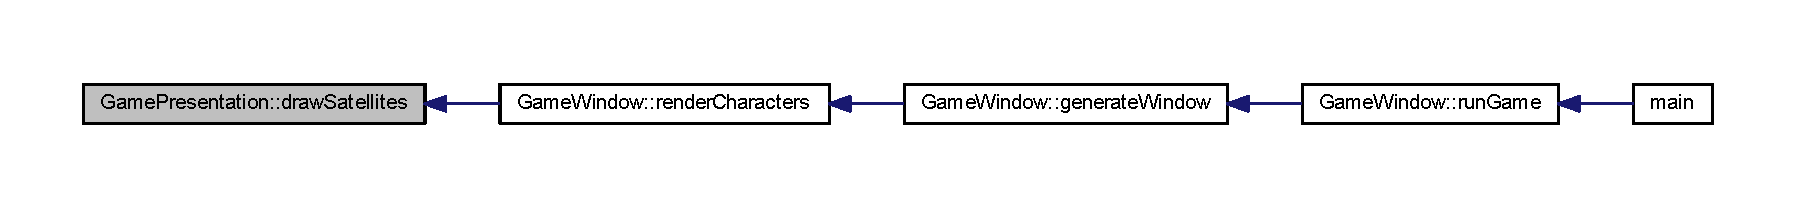
\includegraphics[width=350pt]{class_game_presentation_a7a94467d53b62bd7a83035ea4fa386ac_icgraph}
\end{center}
\end{figure}
\mbox{\Hypertarget{class_game_presentation_a38bab53e3d75b244e14ed2d7c2710fa0}\label{class_game_presentation_a38bab53e3d75b244e14ed2d7c2710fa0}} 
\index{Game\+Presentation@{Game\+Presentation}!draw\+Score\+Presentation@{draw\+Score\+Presentation}}
\index{draw\+Score\+Presentation@{draw\+Score\+Presentation}!Game\+Presentation@{Game\+Presentation}}
\subsubsection{\texorpdfstring{draw\+Score\+Presentation()}{drawScorePresentation()}}
{\footnotesize\ttfamily void Game\+Presentation\+::draw\+Score\+Presentation (\begin{DoxyParamCaption}\item[{Render\+Window \&}]{window }\end{DoxyParamCaption})}

Here is the call graph for this function\+:\nopagebreak
\begin{figure}[H]
\begin{center}
\leavevmode
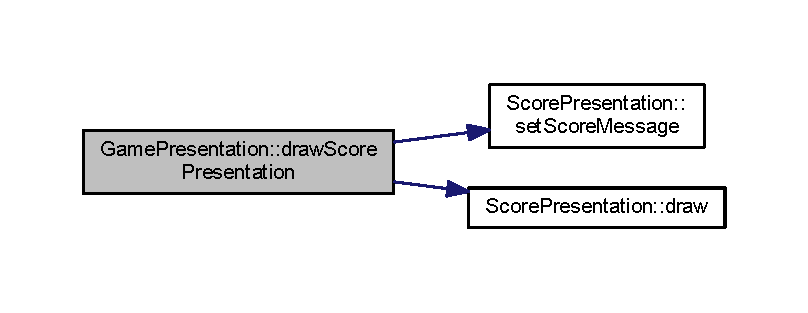
\includegraphics[width=350pt]{class_game_presentation_a38bab53e3d75b244e14ed2d7c2710fa0_cgraph}
\end{center}
\end{figure}
Here is the caller graph for this function\+:\nopagebreak
\begin{figure}[H]
\begin{center}
\leavevmode
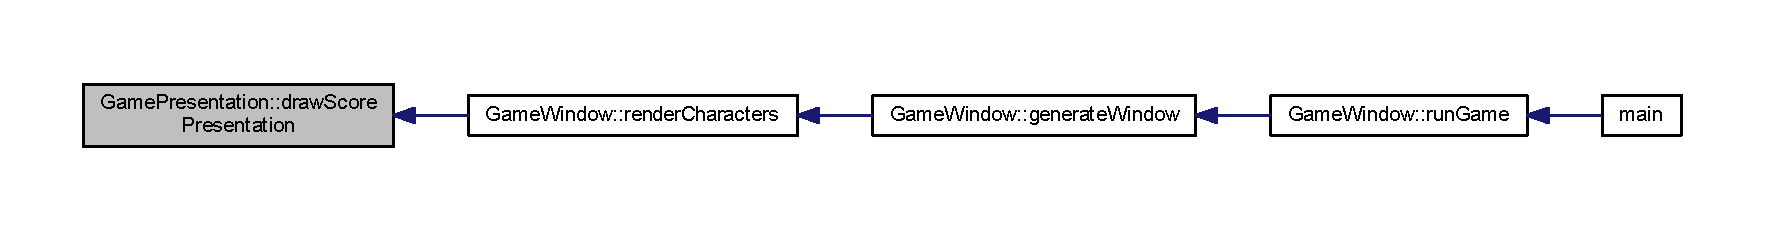
\includegraphics[width=350pt]{class_game_presentation_a38bab53e3d75b244e14ed2d7c2710fa0_icgraph}
\end{center}
\end{figure}
\mbox{\Hypertarget{class_game_presentation_a28a7d4fb65413d6a10b960721aaca0d2}\label{class_game_presentation_a28a7d4fb65413d6a10b960721aaca0d2}} 
\index{Game\+Presentation@{Game\+Presentation}!get\+Asteroid\+Presentation\+Vector@{get\+Asteroid\+Presentation\+Vector}}
\index{get\+Asteroid\+Presentation\+Vector@{get\+Asteroid\+Presentation\+Vector}!Game\+Presentation@{Game\+Presentation}}
\subsubsection{\texorpdfstring{get\+Asteroid\+Presentation\+Vector()}{getAsteroidPresentationVector()}}
{\footnotesize\ttfamily vector$<$ \hyperlink{class_asteroid_presentation}{Asteroid\+Presentation} $>$ Game\+Presentation\+::get\+Asteroid\+Presentation\+Vector (\begin{DoxyParamCaption}{ }\end{DoxyParamCaption})}

Here is the caller graph for this function\+:\nopagebreak
\begin{figure}[H]
\begin{center}
\leavevmode
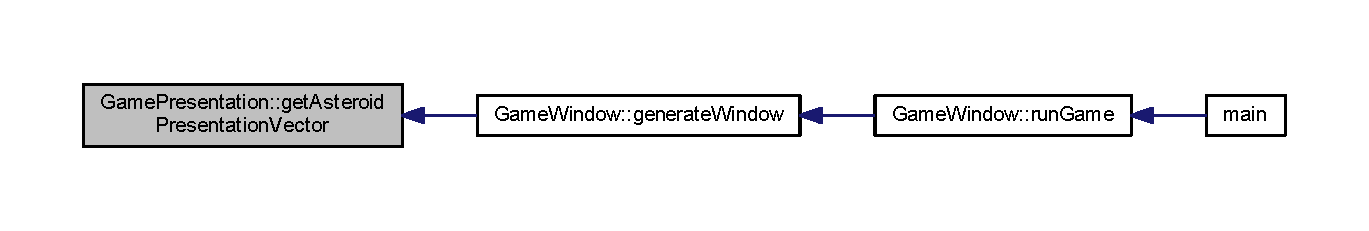
\includegraphics[width=350pt]{class_game_presentation_a28a7d4fb65413d6a10b960721aaca0d2_icgraph}
\end{center}
\end{figure}
\mbox{\Hypertarget{class_game_presentation_ab09fbeaf4a3dfd753f1bce5cdd78969e}\label{class_game_presentation_ab09fbeaf4a3dfd753f1bce5cdd78969e}} 
\index{Game\+Presentation@{Game\+Presentation}!get\+Enemies\+Killed@{get\+Enemies\+Killed}}
\index{get\+Enemies\+Killed@{get\+Enemies\+Killed}!Game\+Presentation@{Game\+Presentation}}
\subsubsection{\texorpdfstring{get\+Enemies\+Killed()}{getEnemiesKilled()}}
{\footnotesize\ttfamily int Game\+Presentation\+::get\+Enemies\+Killed (\begin{DoxyParamCaption}{ }\end{DoxyParamCaption})}

Here is the caller graph for this function\+:\nopagebreak
\begin{figure}[H]
\begin{center}
\leavevmode
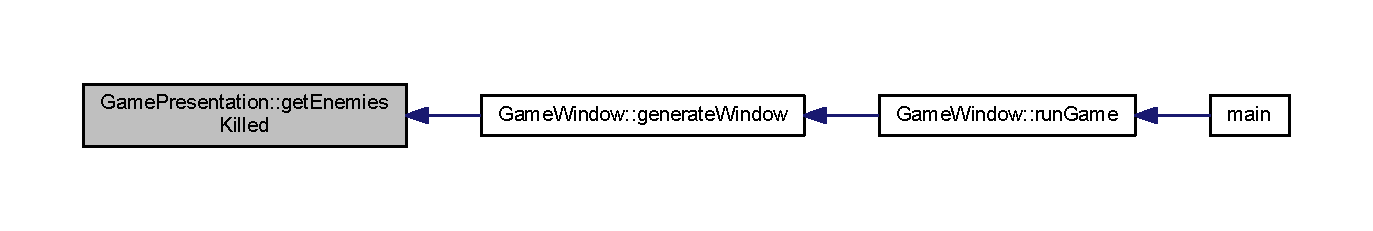
\includegraphics[width=350pt]{class_game_presentation_ab09fbeaf4a3dfd753f1bce5cdd78969e_icgraph}
\end{center}
\end{figure}
\mbox{\Hypertarget{class_game_presentation_a903a8e09c19324b2380b5073abd570f0}\label{class_game_presentation_a903a8e09c19324b2380b5073abd570f0}} 
\index{Game\+Presentation@{Game\+Presentation}!get\+Enemy\+Presentation\+Vector@{get\+Enemy\+Presentation\+Vector}}
\index{get\+Enemy\+Presentation\+Vector@{get\+Enemy\+Presentation\+Vector}!Game\+Presentation@{Game\+Presentation}}
\subsubsection{\texorpdfstring{get\+Enemy\+Presentation\+Vector()}{getEnemyPresentationVector()}}
{\footnotesize\ttfamily vector$<$ \hyperlink{class_enemy_presentation}{Enemy\+Presentation} $>$ Game\+Presentation\+::get\+Enemy\+Presentation\+Vector (\begin{DoxyParamCaption}{ }\end{DoxyParamCaption})}

Here is the caller graph for this function\+:\nopagebreak
\begin{figure}[H]
\begin{center}
\leavevmode
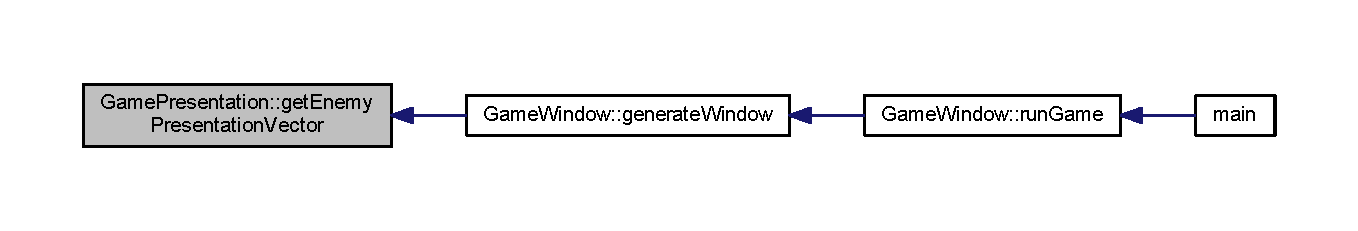
\includegraphics[width=350pt]{class_game_presentation_a903a8e09c19324b2380b5073abd570f0_icgraph}
\end{center}
\end{figure}
\mbox{\Hypertarget{class_game_presentation_a6da88c7baf912bccf09f274b6a5ae7b6}\label{class_game_presentation_a6da88c7baf912bccf09f274b6a5ae7b6}} 
\index{Game\+Presentation@{Game\+Presentation}!get\+Laser\+Generator\+Presentation@{get\+Laser\+Generator\+Presentation}}
\index{get\+Laser\+Generator\+Presentation@{get\+Laser\+Generator\+Presentation}!Game\+Presentation@{Game\+Presentation}}
\subsubsection{\texorpdfstring{get\+Laser\+Generator\+Presentation()}{getLaserGeneratorPresentation()}}
{\footnotesize\ttfamily vector$<$ \hyperlink{class_laser_generator_presentation}{Laser\+Generator\+Presentation} $>$ Game\+Presentation\+::get\+Laser\+Generator\+Presentation (\begin{DoxyParamCaption}{ }\end{DoxyParamCaption})}

Here is the caller graph for this function\+:\nopagebreak
\begin{figure}[H]
\begin{center}
\leavevmode
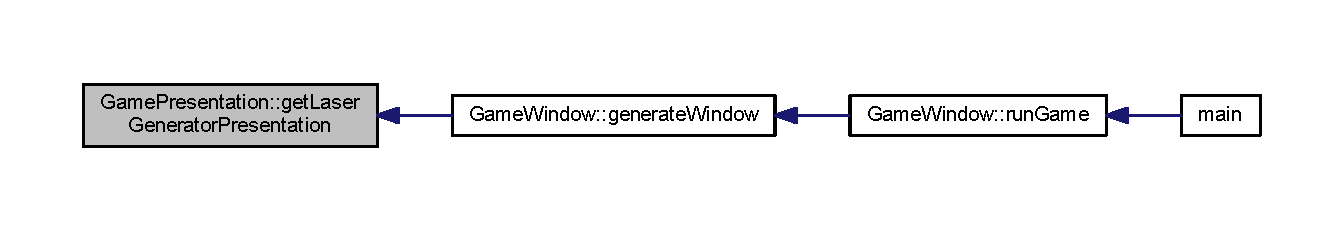
\includegraphics[width=350pt]{class_game_presentation_a6da88c7baf912bccf09f274b6a5ae7b6_icgraph}
\end{center}
\end{figure}
\mbox{\Hypertarget{class_game_presentation_a8bb8847556bd4977479df73eec79b2eb}\label{class_game_presentation_a8bb8847556bd4977479df73eec79b2eb}} 
\index{Game\+Presentation@{Game\+Presentation}!get\+Satellite\+Presentation\+Vector@{get\+Satellite\+Presentation\+Vector}}
\index{get\+Satellite\+Presentation\+Vector@{get\+Satellite\+Presentation\+Vector}!Game\+Presentation@{Game\+Presentation}}
\subsubsection{\texorpdfstring{get\+Satellite\+Presentation\+Vector()}{getSatellitePresentationVector()}}
{\footnotesize\ttfamily vector$<$ \hyperlink{class_satellite_presentation}{Satellite\+Presentation} $>$ Game\+Presentation\+::get\+Satellite\+Presentation\+Vector (\begin{DoxyParamCaption}{ }\end{DoxyParamCaption})}

Here is the caller graph for this function\+:\nopagebreak
\begin{figure}[H]
\begin{center}
\leavevmode
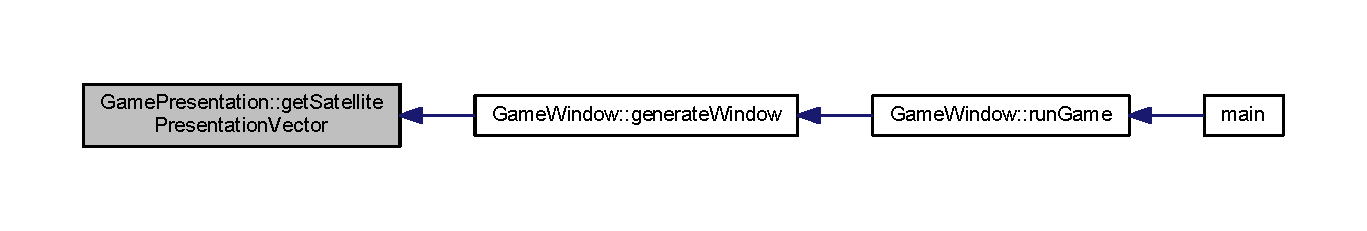
\includegraphics[width=350pt]{class_game_presentation_a8bb8847556bd4977479df73eec79b2eb_icgraph}
\end{center}
\end{figure}
\mbox{\Hypertarget{class_game_presentation_ae2a317ddda3f666fdb1ca4f4c68f6b49}\label{class_game_presentation_ae2a317ddda3f666fdb1ca4f4c68f6b49}} 
\index{Game\+Presentation@{Game\+Presentation}!render\+Sprite@{render\+Sprite}}
\index{render\+Sprite@{render\+Sprite}!Game\+Presentation@{Game\+Presentation}}
\subsubsection{\texorpdfstring{render\+Sprite()}{renderSprite()}}
{\footnotesize\ttfamily void Game\+Presentation\+::render\+Sprite (\begin{DoxyParamCaption}\item[{Render\+Window \&}]{window }\end{DoxyParamCaption})}

Here is the call graph for this function\+:\nopagebreak
\begin{figure}[H]
\begin{center}
\leavevmode
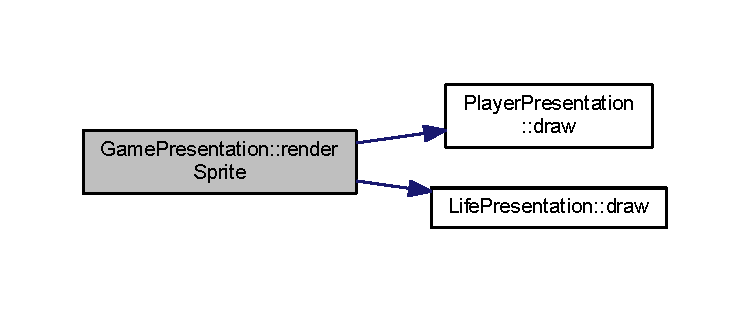
\includegraphics[width=350pt]{class_game_presentation_ae2a317ddda3f666fdb1ca4f4c68f6b49_cgraph}
\end{center}
\end{figure}
Here is the caller graph for this function\+:\nopagebreak
\begin{figure}[H]
\begin{center}
\leavevmode
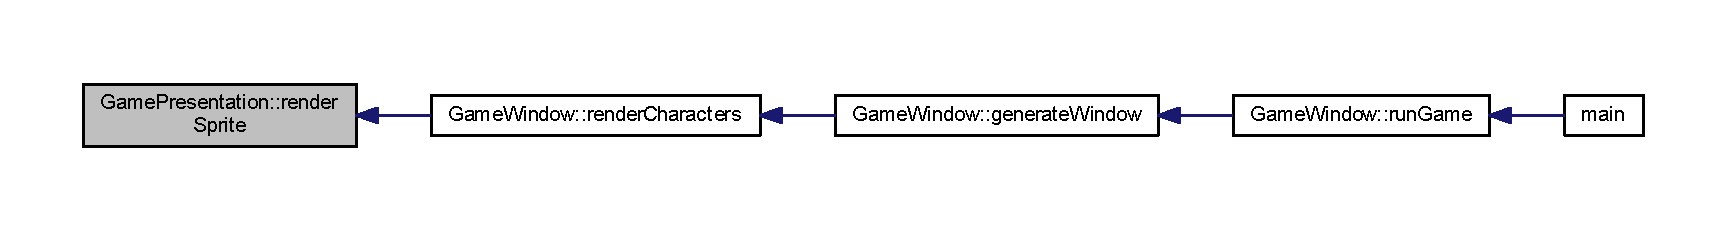
\includegraphics[width=350pt]{class_game_presentation_ae2a317ddda3f666fdb1ca4f4c68f6b49_icgraph}
\end{center}
\end{figure}
\mbox{\Hypertarget{class_game_presentation_a5a329f0403011b464c26218eeff38606}\label{class_game_presentation_a5a329f0403011b464c26218eeff38606}} 
\index{Game\+Presentation@{Game\+Presentation}!set\+Player\+Life\+Count@{set\+Player\+Life\+Count}}
\index{set\+Player\+Life\+Count@{set\+Player\+Life\+Count}!Game\+Presentation@{Game\+Presentation}}
\subsubsection{\texorpdfstring{set\+Player\+Life\+Count()}{setPlayerLifeCount()}}
{\footnotesize\ttfamily void Game\+Presentation\+::set\+Player\+Life\+Count (\begin{DoxyParamCaption}{ }\end{DoxyParamCaption})}

Here is the call graph for this function\+:\nopagebreak
\begin{figure}[H]
\begin{center}
\leavevmode
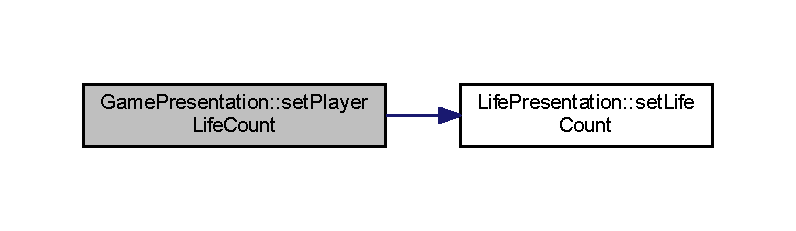
\includegraphics[width=350pt]{class_game_presentation_a5a329f0403011b464c26218eeff38606_cgraph}
\end{center}
\end{figure}
Here is the caller graph for this function\+:\nopagebreak
\begin{figure}[H]
\begin{center}
\leavevmode
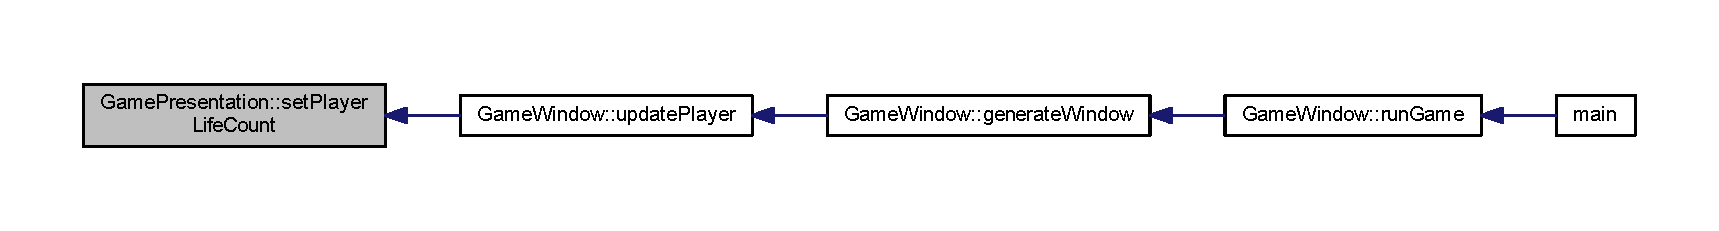
\includegraphics[width=350pt]{class_game_presentation_a5a329f0403011b464c26218eeff38606_icgraph}
\end{center}
\end{figure}
\mbox{\Hypertarget{class_game_presentation_a669fe49aef6332f78a23802cafa6681c}\label{class_game_presentation_a669fe49aef6332f78a23802cafa6681c}} 
\index{Game\+Presentation@{Game\+Presentation}!update\+Asteroid\+Presentation@{update\+Asteroid\+Presentation}}
\index{update\+Asteroid\+Presentation@{update\+Asteroid\+Presentation}!Game\+Presentation@{Game\+Presentation}}
\subsubsection{\texorpdfstring{update\+Asteroid\+Presentation()}{updateAsteroidPresentation()}}
{\footnotesize\ttfamily void Game\+Presentation\+::update\+Asteroid\+Presentation (\begin{DoxyParamCaption}{ }\end{DoxyParamCaption})}

Here is the caller graph for this function\+:\nopagebreak
\begin{figure}[H]
\begin{center}
\leavevmode
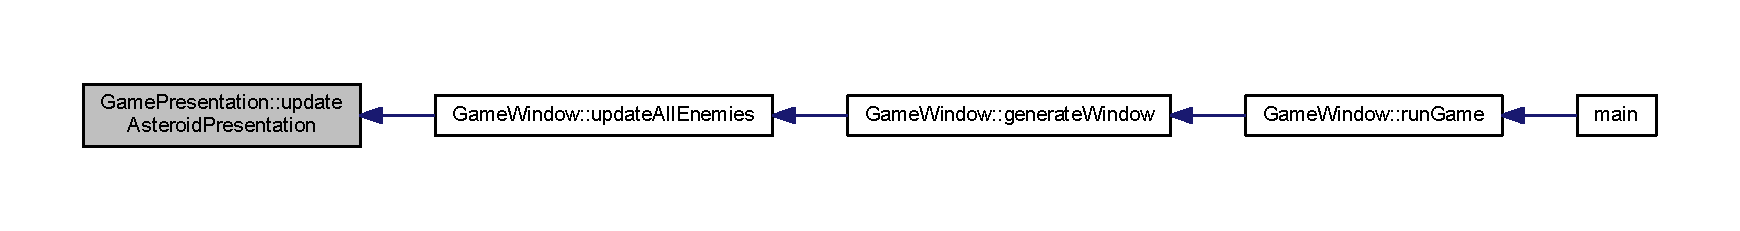
\includegraphics[width=350pt]{class_game_presentation_a669fe49aef6332f78a23802cafa6681c_icgraph}
\end{center}
\end{figure}
\mbox{\Hypertarget{class_game_presentation_a4ab96a6022c08f34aefa62f9a30c1cd8}\label{class_game_presentation_a4ab96a6022c08f34aefa62f9a30c1cd8}} 
\index{Game\+Presentation@{Game\+Presentation}!update\+Enemy\+Presentation@{update\+Enemy\+Presentation}}
\index{update\+Enemy\+Presentation@{update\+Enemy\+Presentation}!Game\+Presentation@{Game\+Presentation}}
\subsubsection{\texorpdfstring{update\+Enemy\+Presentation()}{updateEnemyPresentation()}}
{\footnotesize\ttfamily void Game\+Presentation\+::update\+Enemy\+Presentation (\begin{DoxyParamCaption}{ }\end{DoxyParamCaption})}

Here is the caller graph for this function\+:\nopagebreak
\begin{figure}[H]
\begin{center}
\leavevmode
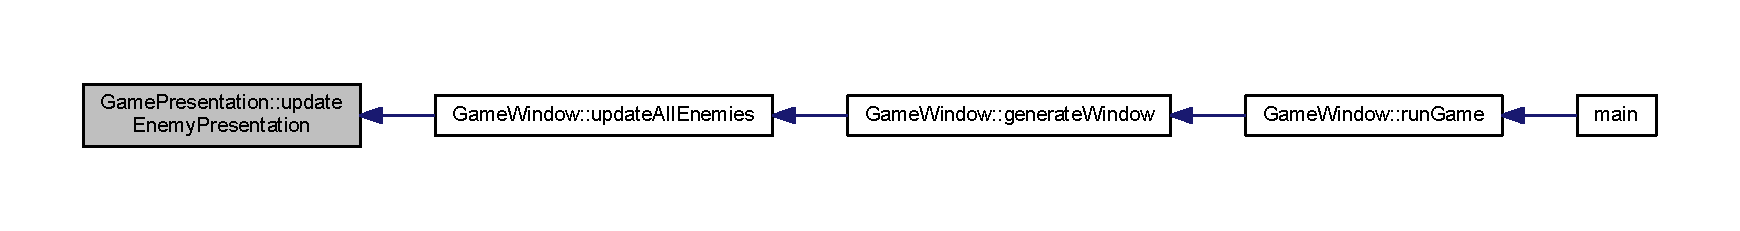
\includegraphics[width=350pt]{class_game_presentation_a4ab96a6022c08f34aefa62f9a30c1cd8_icgraph}
\end{center}
\end{figure}
\mbox{\Hypertarget{class_game_presentation_aa6d8e5e91de557ac2c39bb51e032f14f}\label{class_game_presentation_aa6d8e5e91de557ac2c39bb51e032f14f}} 
\index{Game\+Presentation@{Game\+Presentation}!update\+Laser\+Generator\+Presentation@{update\+Laser\+Generator\+Presentation}}
\index{update\+Laser\+Generator\+Presentation@{update\+Laser\+Generator\+Presentation}!Game\+Presentation@{Game\+Presentation}}
\subsubsection{\texorpdfstring{update\+Laser\+Generator\+Presentation()}{updateLaserGeneratorPresentation()}}
{\footnotesize\ttfamily void Game\+Presentation\+::update\+Laser\+Generator\+Presentation (\begin{DoxyParamCaption}{ }\end{DoxyParamCaption})}

Here is the caller graph for this function\+:\nopagebreak
\begin{figure}[H]
\begin{center}
\leavevmode
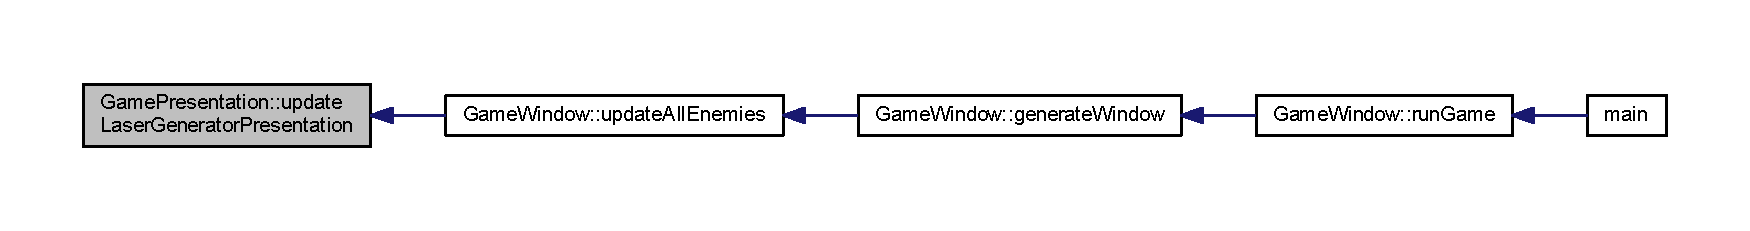
\includegraphics[width=350pt]{class_game_presentation_aa6d8e5e91de557ac2c39bb51e032f14f_icgraph}
\end{center}
\end{figure}
\mbox{\Hypertarget{class_game_presentation_af0a19d50c4099e7a19426cdffa5ebb82}\label{class_game_presentation_af0a19d50c4099e7a19426cdffa5ebb82}} 
\index{Game\+Presentation@{Game\+Presentation}!up\+Date\+Player\+Bullet\+Presentation@{up\+Date\+Player\+Bullet\+Presentation}}
\index{up\+Date\+Player\+Bullet\+Presentation@{up\+Date\+Player\+Bullet\+Presentation}!Game\+Presentation@{Game\+Presentation}}
\subsubsection{\texorpdfstring{up\+Date\+Player\+Bullet\+Presentation()}{upDatePlayerBulletPresentation()}}
{\footnotesize\ttfamily void Game\+Presentation\+::up\+Date\+Player\+Bullet\+Presentation (\begin{DoxyParamCaption}{ }\end{DoxyParamCaption})}

Here is the caller graph for this function\+:\nopagebreak
\begin{figure}[H]
\begin{center}
\leavevmode
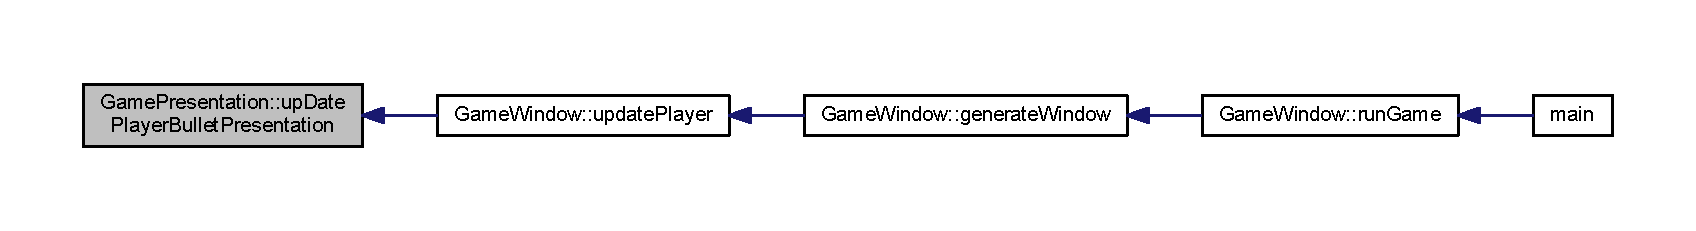
\includegraphics[width=350pt]{class_game_presentation_af0a19d50c4099e7a19426cdffa5ebb82_icgraph}
\end{center}
\end{figure}
\mbox{\Hypertarget{class_game_presentation_a08abc97c6f65eda4ac7c54d55a9054b4}\label{class_game_presentation_a08abc97c6f65eda4ac7c54d55a9054b4}} 
\index{Game\+Presentation@{Game\+Presentation}!up\+Date\+Player\+Position@{up\+Date\+Player\+Position}}
\index{up\+Date\+Player\+Position@{up\+Date\+Player\+Position}!Game\+Presentation@{Game\+Presentation}}
\subsubsection{\texorpdfstring{up\+Date\+Player\+Position()}{upDatePlayerPosition()}}
{\footnotesize\ttfamily void Game\+Presentation\+::up\+Date\+Player\+Position (\begin{DoxyParamCaption}{ }\end{DoxyParamCaption})}

Here is the call graph for this function\+:\nopagebreak
\begin{figure}[H]
\begin{center}
\leavevmode
\includegraphics[width=350pt]{class_game_presentation_a08abc97c6f65eda4ac7c54d55a9054b4_cgraph}
\end{center}
\end{figure}
Here is the caller graph for this function\+:\nopagebreak
\begin{figure}[H]
\begin{center}
\leavevmode
\includegraphics[width=350pt]{class_game_presentation_a08abc97c6f65eda4ac7c54d55a9054b4_icgraph}
\end{center}
\end{figure}
\mbox{\Hypertarget{class_game_presentation_ab2cf74842583bf5b63e5973fb8b657be}\label{class_game_presentation_ab2cf74842583bf5b63e5973fb8b657be}} 
\index{Game\+Presentation@{Game\+Presentation}!update\+Score\+Presentation@{update\+Score\+Presentation}}
\index{update\+Score\+Presentation@{update\+Score\+Presentation}!Game\+Presentation@{Game\+Presentation}}
\subsubsection{\texorpdfstring{update\+Score\+Presentation()}{updateScorePresentation()}}
{\footnotesize\ttfamily void Game\+Presentation\+::update\+Score\+Presentation (\begin{DoxyParamCaption}{ }\end{DoxyParamCaption})}

Here is the call graph for this function\+:\nopagebreak
\begin{figure}[H]
\begin{center}
\leavevmode
\includegraphics[width=350pt]{class_game_presentation_ab2cf74842583bf5b63e5973fb8b657be_cgraph}
\end{center}
\end{figure}
Here is the caller graph for this function\+:\nopagebreak
\begin{figure}[H]
\begin{center}
\leavevmode
\includegraphics[width=350pt]{class_game_presentation_ab2cf74842583bf5b63e5973fb8b657be_icgraph}
\end{center}
\end{figure}


\subsection{Member Data Documentation}
\mbox{\Hypertarget{class_game_presentation_a2f149f73bdd87ded8a6d66ecc427352f}\label{class_game_presentation_a2f149f73bdd87ded8a6d66ecc427352f}} 
\index{Game\+Presentation@{Game\+Presentation}!game\+Logic\+\_\+shared\+\_\+pointer@{game\+Logic\+\_\+shared\+\_\+pointer}}
\index{game\+Logic\+\_\+shared\+\_\+pointer@{game\+Logic\+\_\+shared\+\_\+pointer}!Game\+Presentation@{Game\+Presentation}}
\subsubsection{\texorpdfstring{game\+Logic\+\_\+shared\+\_\+pointer}{gameLogic\_shared\_pointer}}
{\footnotesize\ttfamily shared\+\_\+ptr$<$\hyperlink{class_game_logic}{Game\+Logic}$>$ Game\+Presentation\+::game\+Logic\+\_\+shared\+\_\+pointer}



The documentation for this class was generated from the following files\+:\begin{DoxyCompactItemize}
\item 
C\+:/\+Users/\+User/\+Documents/\+Software\+Dev2\+Project/\+Space\+Rider\+Project/\hyperlink{_game_presentation_8h}{Game\+Presentation.\+h}\item 
C\+:/\+Users/\+User/\+Documents/\+Software\+Dev2\+Project/\+Space\+Rider\+Project/\hyperlink{_game_presentation_8cpp}{Game\+Presentation.\+cpp}\end{DoxyCompactItemize}

\hypertarget{class_game_window}{}\section{Game\+Window Class Reference}
\label{class_game_window}\index{Game\+Window@{Game\+Window}}


{\ttfamily \#include $<$Game\+Window.\+h$>$}

\subsection*{Public Member Functions}
\begin{DoxyCompactItemize}
\item 
\hyperlink{class_game_window_a81f2f6fea59b4723569c591756328163}{Game\+Window} ()
\item 
void \hyperlink{class_game_window_a6d969bf2a5284c731c5ba3eb03d4e3a1}{check\+Key\+Board\+Event} ()
\item 
void \hyperlink{class_game_window_a43f64127a3b8836405f80242c1e997f4}{generate\+Window} ()
\item 
void \hyperlink{class_game_window_ac32c7b2e85e30f5bab516551c6277c3a}{render\+Characters} (Render\+Window \&window)
\item 
void \hyperlink{class_game_window_a119f405a2ff052c74d902c5b02bf0f05}{fire\+Player\+Bullet} ()
\item 
void \hyperlink{class_game_window_a9ebcf385e9ed9fd52f1d8b2c88f9c091}{update\+Player} ()
\item 
void \hyperlink{class_game_window_a62ed57d80a4eb7945777f5d383747bdf}{update\+All\+Enemies} ()
\item 
void \hyperlink{class_game_window_aa4188b605313be96d69cf32d3f143987}{run\+Game} ()
\end{DoxyCompactItemize}


\subsection{Constructor \& Destructor Documentation}
\mbox{\Hypertarget{class_game_window_a81f2f6fea59b4723569c591756328163}\label{class_game_window_a81f2f6fea59b4723569c591756328163}} 
\index{Game\+Window@{Game\+Window}!Game\+Window@{Game\+Window}}
\index{Game\+Window@{Game\+Window}!Game\+Window@{Game\+Window}}
\subsubsection{\texorpdfstring{Game\+Window()}{GameWindow()}}
{\footnotesize\ttfamily Game\+Window\+::\+Game\+Window (\begin{DoxyParamCaption}{ }\end{DoxyParamCaption})}



\subsection{Member Function Documentation}
\mbox{\Hypertarget{class_game_window_a6d969bf2a5284c731c5ba3eb03d4e3a1}\label{class_game_window_a6d969bf2a5284c731c5ba3eb03d4e3a1}} 
\index{Game\+Window@{Game\+Window}!check\+Key\+Board\+Event@{check\+Key\+Board\+Event}}
\index{check\+Key\+Board\+Event@{check\+Key\+Board\+Event}!Game\+Window@{Game\+Window}}
\subsubsection{\texorpdfstring{check\+Key\+Board\+Event()}{checkKeyBoardEvent()}}
{\footnotesize\ttfamily void Game\+Window\+::check\+Key\+Board\+Event (\begin{DoxyParamCaption}{ }\end{DoxyParamCaption})}

Here is the call graph for this function\+:\nopagebreak
\begin{figure}[H]
\begin{center}
\leavevmode
\includegraphics[width=350pt]{class_game_window_a6d969bf2a5284c731c5ba3eb03d4e3a1_cgraph}
\end{center}
\end{figure}
Here is the caller graph for this function\+:\nopagebreak
\begin{figure}[H]
\begin{center}
\leavevmode
\includegraphics[width=350pt]{class_game_window_a6d969bf2a5284c731c5ba3eb03d4e3a1_icgraph}
\end{center}
\end{figure}
\mbox{\Hypertarget{class_game_window_a119f405a2ff052c74d902c5b02bf0f05}\label{class_game_window_a119f405a2ff052c74d902c5b02bf0f05}} 
\index{Game\+Window@{Game\+Window}!fire\+Player\+Bullet@{fire\+Player\+Bullet}}
\index{fire\+Player\+Bullet@{fire\+Player\+Bullet}!Game\+Window@{Game\+Window}}
\subsubsection{\texorpdfstring{fire\+Player\+Bullet()}{firePlayerBullet()}}
{\footnotesize\ttfamily void Game\+Window\+::fire\+Player\+Bullet (\begin{DoxyParamCaption}{ }\end{DoxyParamCaption})}

Here is the call graph for this function\+:\nopagebreak
\begin{figure}[H]
\begin{center}
\leavevmode
\includegraphics[width=350pt]{class_game_window_a119f405a2ff052c74d902c5b02bf0f05_cgraph}
\end{center}
\end{figure}
Here is the caller graph for this function\+:\nopagebreak
\begin{figure}[H]
\begin{center}
\leavevmode
\includegraphics[width=350pt]{class_game_window_a119f405a2ff052c74d902c5b02bf0f05_icgraph}
\end{center}
\end{figure}
\mbox{\Hypertarget{class_game_window_a43f64127a3b8836405f80242c1e997f4}\label{class_game_window_a43f64127a3b8836405f80242c1e997f4}} 
\index{Game\+Window@{Game\+Window}!generate\+Window@{generate\+Window}}
\index{generate\+Window@{generate\+Window}!Game\+Window@{Game\+Window}}
\subsubsection{\texorpdfstring{generate\+Window()}{generateWindow()}}
{\footnotesize\ttfamily void Game\+Window\+::generate\+Window (\begin{DoxyParamCaption}{ }\end{DoxyParamCaption})}

Here is the call graph for this function\+:\nopagebreak
\begin{figure}[H]
\begin{center}
\leavevmode
\includegraphics[width=350pt]{class_game_window_a43f64127a3b8836405f80242c1e997f4_cgraph}
\end{center}
\end{figure}
Here is the caller graph for this function\+:\nopagebreak
\begin{figure}[H]
\begin{center}
\leavevmode
\includegraphics[width=350pt]{class_game_window_a43f64127a3b8836405f80242c1e997f4_icgraph}
\end{center}
\end{figure}
\mbox{\Hypertarget{class_game_window_ac32c7b2e85e30f5bab516551c6277c3a}\label{class_game_window_ac32c7b2e85e30f5bab516551c6277c3a}} 
\index{Game\+Window@{Game\+Window}!render\+Characters@{render\+Characters}}
\index{render\+Characters@{render\+Characters}!Game\+Window@{Game\+Window}}
\subsubsection{\texorpdfstring{render\+Characters()}{renderCharacters()}}
{\footnotesize\ttfamily void Game\+Window\+::render\+Characters (\begin{DoxyParamCaption}\item[{Render\+Window \&}]{window }\end{DoxyParamCaption})}

Here is the call graph for this function\+:\nopagebreak
\begin{figure}[H]
\begin{center}
\leavevmode
\includegraphics[width=350pt]{class_game_window_ac32c7b2e85e30f5bab516551c6277c3a_cgraph}
\end{center}
\end{figure}
Here is the caller graph for this function\+:\nopagebreak
\begin{figure}[H]
\begin{center}
\leavevmode
\includegraphics[width=350pt]{class_game_window_ac32c7b2e85e30f5bab516551c6277c3a_icgraph}
\end{center}
\end{figure}
\mbox{\Hypertarget{class_game_window_aa4188b605313be96d69cf32d3f143987}\label{class_game_window_aa4188b605313be96d69cf32d3f143987}} 
\index{Game\+Window@{Game\+Window}!run\+Game@{run\+Game}}
\index{run\+Game@{run\+Game}!Game\+Window@{Game\+Window}}
\subsubsection{\texorpdfstring{run\+Game()}{runGame()}}
{\footnotesize\ttfamily void Game\+Window\+::run\+Game (\begin{DoxyParamCaption}{ }\end{DoxyParamCaption})}

Here is the call graph for this function\+:\nopagebreak
\begin{figure}[H]
\begin{center}
\leavevmode
\includegraphics[width=350pt]{class_game_window_aa4188b605313be96d69cf32d3f143987_cgraph}
\end{center}
\end{figure}
Here is the caller graph for this function\+:\nopagebreak
\begin{figure}[H]
\begin{center}
\leavevmode
\includegraphics[width=277pt]{class_game_window_aa4188b605313be96d69cf32d3f143987_icgraph}
\end{center}
\end{figure}
\mbox{\Hypertarget{class_game_window_a62ed57d80a4eb7945777f5d383747bdf}\label{class_game_window_a62ed57d80a4eb7945777f5d383747bdf}} 
\index{Game\+Window@{Game\+Window}!update\+All\+Enemies@{update\+All\+Enemies}}
\index{update\+All\+Enemies@{update\+All\+Enemies}!Game\+Window@{Game\+Window}}
\subsubsection{\texorpdfstring{update\+All\+Enemies()}{updateAllEnemies()}}
{\footnotesize\ttfamily void Game\+Window\+::update\+All\+Enemies (\begin{DoxyParamCaption}{ }\end{DoxyParamCaption})}

Here is the call graph for this function\+:\nopagebreak
\begin{figure}[H]
\begin{center}
\leavevmode
\includegraphics[width=350pt]{class_game_window_a62ed57d80a4eb7945777f5d383747bdf_cgraph}
\end{center}
\end{figure}
Here is the caller graph for this function\+:\nopagebreak
\begin{figure}[H]
\begin{center}
\leavevmode
\includegraphics[width=350pt]{class_game_window_a62ed57d80a4eb7945777f5d383747bdf_icgraph}
\end{center}
\end{figure}
\mbox{\Hypertarget{class_game_window_a9ebcf385e9ed9fd52f1d8b2c88f9c091}\label{class_game_window_a9ebcf385e9ed9fd52f1d8b2c88f9c091}} 
\index{Game\+Window@{Game\+Window}!update\+Player@{update\+Player}}
\index{update\+Player@{update\+Player}!Game\+Window@{Game\+Window}}
\subsubsection{\texorpdfstring{update\+Player()}{updatePlayer()}}
{\footnotesize\ttfamily void Game\+Window\+::update\+Player (\begin{DoxyParamCaption}{ }\end{DoxyParamCaption})}

Here is the call graph for this function\+:\nopagebreak
\begin{figure}[H]
\begin{center}
\leavevmode
\includegraphics[width=350pt]{class_game_window_a9ebcf385e9ed9fd52f1d8b2c88f9c091_cgraph}
\end{center}
\end{figure}
Here is the caller graph for this function\+:\nopagebreak
\begin{figure}[H]
\begin{center}
\leavevmode
\includegraphics[width=350pt]{class_game_window_a9ebcf385e9ed9fd52f1d8b2c88f9c091_icgraph}
\end{center}
\end{figure}


The documentation for this class was generated from the following files\+:\begin{DoxyCompactItemize}
\item 
C\+:/\+Users/\+User/\+Documents/\+Software\+Dev2\+Project/\+Space\+Rider\+Project/\hyperlink{_game_window_8h}{Game\+Window.\+h}\item 
C\+:/\+Users/\+User/\+Documents/\+Software\+Dev2\+Project/\+Space\+Rider\+Project/\hyperlink{_game_window_8cpp}{Game\+Window.\+cpp}\end{DoxyCompactItemize}

\hypertarget{class_i_bullet}{}\section{I\+Bullet Class Reference}
\label{class_i_bullet}\index{I\+Bullet@{I\+Bullet}}
Inheritance diagram for I\+Bullet\+:\begin{figure}[H]
\begin{center}
\leavevmode
\includegraphics[height=3.000000cm]{class_i_bullet}
\end{center}
\end{figure}
\subsection*{Public Member Functions}
\begin{DoxyCompactItemize}
\item 
\mbox{\Hypertarget{class_i_bullet_a0884074f0bc793fb5a52ac33842622fd}\label{class_i_bullet_a0884074f0bc793fb5a52ac33842622fd}} 
virtual void {\bfseries move} ()=0
\item 
\mbox{\Hypertarget{class_i_bullet_a072298555accb47f11b84f4c781ae876}\label{class_i_bullet_a072298555accb47f11b84f4c781ae876}} 
virtual void {\bfseries set\+Damage} (int damage)=0
\item 
\mbox{\Hypertarget{class_i_bullet_ab6643a4ad3888ee4ebfbc3d445c4b73d}\label{class_i_bullet_ab6643a4ad3888ee4ebfbc3d445c4b73d}} 
virtual int {\bfseries get\+Damage} ()=0
\item 
\mbox{\Hypertarget{class_i_bullet_ac1252496738126ec94a97512011b9112}\label{class_i_bullet_ac1252496738126ec94a97512011b9112}} 
virtual bool {\bfseries is\+Alive} ()=0
\item 
\mbox{\Hypertarget{class_i_bullet_a20babdd6c657ddda175e84a56564dcfa}\label{class_i_bullet_a20babdd6c657ddda175e84a56564dcfa}} 
virtual float {\bfseries get\+Xposition} ()=0
\item 
\mbox{\Hypertarget{class_i_bullet_a36594de9a0c0ddd7083bca10ef5d8332}\label{class_i_bullet_a36594de9a0c0ddd7083bca10ef5d8332}} 
virtual float {\bfseries get\+Yposition} ()=0
\item 
\mbox{\Hypertarget{class_i_bullet_abf99befdaa121e7c9ca2acc2ed75b513}\label{class_i_bullet_abf99befdaa121e7c9ca2acc2ed75b513}} 
virtual void {\bfseries set\+Life} (bool life)=0
\item 
\mbox{\Hypertarget{class_i_bullet_a327968e71126cdea5998076d8919354f}\label{class_i_bullet_a327968e71126cdea5998076d8919354f}} 
virtual float {\bfseries get\+Radius} ()=0
\item 
\mbox{\Hypertarget{class_i_bullet_a43a43e2df81e05a03be42d9025e6dd2a}\label{class_i_bullet_a43a43e2df81e05a03be42d9025e6dd2a}} 
virtual float {\bfseries get\+Center\+X\+Position} ()=0
\item 
\mbox{\Hypertarget{class_i_bullet_a8245ed2bc72beed1d69547ce5f87a021}\label{class_i_bullet_a8245ed2bc72beed1d69547ce5f87a021}} 
virtual float {\bfseries get\+Center\+Y\+Position} ()=0
\end{DoxyCompactItemize}


The documentation for this class was generated from the following file\+:\begin{DoxyCompactItemize}
\item 
C\+:/\+Users/\+William/\+Documents/\+E\+L\+E\+N3009/\+Space\+Rider\+Project/I\+Bullet.\+h\end{DoxyCompactItemize}

\hypertarget{class_i_enemy}{}\section{I\+Enemy Class Reference}
\label{class_i_enemy}\index{I\+Enemy@{I\+Enemy}}


{\ttfamily \#include $<$I\+Enemy.\+h$>$}



Inheritance diagram for I\+Enemy\+:\nopagebreak
\begin{figure}[H]
\begin{center}
\leavevmode
\includegraphics[width=246pt]{class_i_enemy__inherit__graph}
\end{center}
\end{figure}


Collaboration diagram for I\+Enemy\+:\nopagebreak
\begin{figure}[H]
\begin{center}
\leavevmode
\includegraphics[width=184pt]{class_i_enemy__coll__graph}
\end{center}
\end{figure}
\subsection*{Public Member Functions}
\begin{DoxyCompactItemize}
\item 
virtual void \hyperlink{class_i_enemy_a0dbed8e8e15436305b6ede08b618c232}{move} ()=0
\item 
virtual float \hyperlink{class_i_enemy_a8a9780d5db69d910f264fd7ab89ebee6}{get\+Angleof\+Rotation} ()=0
\item 
virtual bool \hyperlink{class_i_enemy_a3e44ca5e5fabcfd71b26657eba26e5a2}{is\+Alive} ()=0
\item 
virtual void \hyperlink{class_i_enemy_acbc451cafee99cb405d9d9248820b6ea}{reduce\+Health} (int \+\_\+damage)=0
\item 
virtual float \hyperlink{class_i_enemy_a504ea7fa77b8984d5b9dd71352876943}{get\+Xposition} ()=0
\item 
virtual float \hyperlink{class_i_enemy_a8011be7f510f6630250f8b9529815773}{get\+Yposition} ()=0
\item 
virtual void \hyperlink{class_i_enemy_ab58f2f6c2a8c08730aaf8771f088e1bf}{set\+Life} (bool life)=0
\item 
virtual float \hyperlink{class_i_enemy_ab1fb8f6320916ef6a1497f9651704d05}{get\+Radius} ()=0
\item 
virtual float \hyperlink{class_i_enemy_ab5bc39484a8aeaf278c3d127ec5d9545}{get\+Center\+X\+Position} ()=0
\item 
virtual float \hyperlink{class_i_enemy_ac9a2d69103fa86d8344aa368fb33c714}{get\+Center\+Y\+Position} ()=0
\end{DoxyCompactItemize}


\subsection{Member Function Documentation}
\mbox{\Hypertarget{class_i_enemy_a8a9780d5db69d910f264fd7ab89ebee6}\label{class_i_enemy_a8a9780d5db69d910f264fd7ab89ebee6}} 
\index{I\+Enemy@{I\+Enemy}!get\+Angleof\+Rotation@{get\+Angleof\+Rotation}}
\index{get\+Angleof\+Rotation@{get\+Angleof\+Rotation}!I\+Enemy@{I\+Enemy}}
\subsubsection{\texorpdfstring{get\+Angleof\+Rotation()}{getAngleofRotation()}}
{\footnotesize\ttfamily virtual float I\+Enemy\+::get\+Angleof\+Rotation (\begin{DoxyParamCaption}{ }\end{DoxyParamCaption})\hspace{0.3cm}{\ttfamily [pure virtual]}}



Implemented in \hyperlink{class_enemy_logic_ade03be41505c71de49f20fc855c8fede}{Enemy\+Logic}, and \hyperlink{class_asteroid_logic_a2087d2a3b9bf9e6f1367833454b2fb97}{Asteroid\+Logic}.

\mbox{\Hypertarget{class_i_enemy_ab5bc39484a8aeaf278c3d127ec5d9545}\label{class_i_enemy_ab5bc39484a8aeaf278c3d127ec5d9545}} 
\index{I\+Enemy@{I\+Enemy}!get\+Center\+X\+Position@{get\+Center\+X\+Position}}
\index{get\+Center\+X\+Position@{get\+Center\+X\+Position}!I\+Enemy@{I\+Enemy}}
\subsubsection{\texorpdfstring{get\+Center\+X\+Position()}{getCenterXPosition()}}
{\footnotesize\ttfamily virtual float I\+Enemy\+::get\+Center\+X\+Position (\begin{DoxyParamCaption}{ }\end{DoxyParamCaption})\hspace{0.3cm}{\ttfamily [pure virtual]}}



Implements \hyperlink{class_i_moving_game_object_ae4e6c21094ef1e2db32729270c8a7999}{I\+Moving\+Game\+Object}.



Implemented in \hyperlink{class_enemy_logic_a1429e91a81da7646d9b0280f26519d8c}{Enemy\+Logic}, and \hyperlink{class_asteroid_logic_a4bff0373a2cefe48c984b469ddbcb52d}{Asteroid\+Logic}.

\mbox{\Hypertarget{class_i_enemy_ac9a2d69103fa86d8344aa368fb33c714}\label{class_i_enemy_ac9a2d69103fa86d8344aa368fb33c714}} 
\index{I\+Enemy@{I\+Enemy}!get\+Center\+Y\+Position@{get\+Center\+Y\+Position}}
\index{get\+Center\+Y\+Position@{get\+Center\+Y\+Position}!I\+Enemy@{I\+Enemy}}
\subsubsection{\texorpdfstring{get\+Center\+Y\+Position()}{getCenterYPosition()}}
{\footnotesize\ttfamily virtual float I\+Enemy\+::get\+Center\+Y\+Position (\begin{DoxyParamCaption}{ }\end{DoxyParamCaption})\hspace{0.3cm}{\ttfamily [pure virtual]}}



Implements \hyperlink{class_i_moving_game_object_a075f69d69fd38dc02a0ec3c7b1cb0534}{I\+Moving\+Game\+Object}.



Implemented in \hyperlink{class_enemy_logic_a8eb47a87a47288783e0c8963c39d24e4}{Enemy\+Logic}, and \hyperlink{class_asteroid_logic_a00c9cda893b9dee7e2225377dd54a2eb}{Asteroid\+Logic}.

\mbox{\Hypertarget{class_i_enemy_ab1fb8f6320916ef6a1497f9651704d05}\label{class_i_enemy_ab1fb8f6320916ef6a1497f9651704d05}} 
\index{I\+Enemy@{I\+Enemy}!get\+Radius@{get\+Radius}}
\index{get\+Radius@{get\+Radius}!I\+Enemy@{I\+Enemy}}
\subsubsection{\texorpdfstring{get\+Radius()}{getRadius()}}
{\footnotesize\ttfamily virtual float I\+Enemy\+::get\+Radius (\begin{DoxyParamCaption}{ }\end{DoxyParamCaption})\hspace{0.3cm}{\ttfamily [pure virtual]}}



Implements \hyperlink{class_i_moving_game_object_ab2120f126d088beda46654aa3ccfd705}{I\+Moving\+Game\+Object}.



Implemented in \hyperlink{class_enemy_logic_ab6736c870e69bc20bef8d6d010946eb2}{Enemy\+Logic}, and \hyperlink{class_asteroid_logic_a575d9f801770906960b65dafe937fba5}{Asteroid\+Logic}.

\mbox{\Hypertarget{class_i_enemy_a504ea7fa77b8984d5b9dd71352876943}\label{class_i_enemy_a504ea7fa77b8984d5b9dd71352876943}} 
\index{I\+Enemy@{I\+Enemy}!get\+Xposition@{get\+Xposition}}
\index{get\+Xposition@{get\+Xposition}!I\+Enemy@{I\+Enemy}}
\subsubsection{\texorpdfstring{get\+Xposition()}{getXposition()}}
{\footnotesize\ttfamily virtual float I\+Enemy\+::get\+Xposition (\begin{DoxyParamCaption}{ }\end{DoxyParamCaption})\hspace{0.3cm}{\ttfamily [pure virtual]}}



Implements \hyperlink{class_i_moving_game_object_acc7f0195491b1843558c8c558cbc7363}{I\+Moving\+Game\+Object}.



Implemented in \hyperlink{class_enemy_logic_a7eed969ab8e3d2527cdac04ef39a5aba}{Enemy\+Logic}, and \hyperlink{class_asteroid_logic_a1d79a614c5e1a9409404f6a2def25761}{Asteroid\+Logic}.

\mbox{\Hypertarget{class_i_enemy_a8011be7f510f6630250f8b9529815773}\label{class_i_enemy_a8011be7f510f6630250f8b9529815773}} 
\index{I\+Enemy@{I\+Enemy}!get\+Yposition@{get\+Yposition}}
\index{get\+Yposition@{get\+Yposition}!I\+Enemy@{I\+Enemy}}
\subsubsection{\texorpdfstring{get\+Yposition()}{getYposition()}}
{\footnotesize\ttfamily virtual float I\+Enemy\+::get\+Yposition (\begin{DoxyParamCaption}{ }\end{DoxyParamCaption})\hspace{0.3cm}{\ttfamily [pure virtual]}}



Implements \hyperlink{class_i_moving_game_object_a153c0017219e17262a9cceddba3f61d6}{I\+Moving\+Game\+Object}.



Implemented in \hyperlink{class_enemy_logic_ae614032054926a4a25ed56f61111392b}{Enemy\+Logic}, and \hyperlink{class_asteroid_logic_a83863c5262a29b2999d04ad443622bbc}{Asteroid\+Logic}.

\mbox{\Hypertarget{class_i_enemy_a3e44ca5e5fabcfd71b26657eba26e5a2}\label{class_i_enemy_a3e44ca5e5fabcfd71b26657eba26e5a2}} 
\index{I\+Enemy@{I\+Enemy}!is\+Alive@{is\+Alive}}
\index{is\+Alive@{is\+Alive}!I\+Enemy@{I\+Enemy}}
\subsubsection{\texorpdfstring{is\+Alive()}{isAlive()}}
{\footnotesize\ttfamily virtual bool I\+Enemy\+::is\+Alive (\begin{DoxyParamCaption}{ }\end{DoxyParamCaption})\hspace{0.3cm}{\ttfamily [pure virtual]}}



Implements \hyperlink{class_i_moving_game_object_ab88f75c872699dd1376e5e83f6188e34}{I\+Moving\+Game\+Object}.



Implemented in \hyperlink{class_enemy_logic_a8dd48fa112c41249e46728d7ec8f820e}{Enemy\+Logic}, and \hyperlink{class_asteroid_logic_a18e01f832db4f109799fc01c8c15efcd}{Asteroid\+Logic}.

\mbox{\Hypertarget{class_i_enemy_a0dbed8e8e15436305b6ede08b618c232}\label{class_i_enemy_a0dbed8e8e15436305b6ede08b618c232}} 
\index{I\+Enemy@{I\+Enemy}!move@{move}}
\index{move@{move}!I\+Enemy@{I\+Enemy}}
\subsubsection{\texorpdfstring{move()}{move()}}
{\footnotesize\ttfamily virtual void I\+Enemy\+::move (\begin{DoxyParamCaption}{ }\end{DoxyParamCaption})\hspace{0.3cm}{\ttfamily [pure virtual]}}



Implemented in \hyperlink{class_enemy_logic_a2bc8ba642d677ab31f4b54ec00299e25}{Enemy\+Logic}, and \hyperlink{class_asteroid_logic_af20b202c4f5857279192733a0b2fdbd3}{Asteroid\+Logic}.

\mbox{\Hypertarget{class_i_enemy_acbc451cafee99cb405d9d9248820b6ea}\label{class_i_enemy_acbc451cafee99cb405d9d9248820b6ea}} 
\index{I\+Enemy@{I\+Enemy}!reduce\+Health@{reduce\+Health}}
\index{reduce\+Health@{reduce\+Health}!I\+Enemy@{I\+Enemy}}
\subsubsection{\texorpdfstring{reduce\+Health()}{reduceHealth()}}
{\footnotesize\ttfamily virtual void I\+Enemy\+::reduce\+Health (\begin{DoxyParamCaption}\item[{int}]{\+\_\+damage }\end{DoxyParamCaption})\hspace{0.3cm}{\ttfamily [pure virtual]}}



Implemented in \hyperlink{class_enemy_logic_aaf2f8ff785c8f7410e04cfb3cb192b9b}{Enemy\+Logic}, and \hyperlink{class_asteroid_logic_a54519e4b2719c70d17f5a28bb0d8fb56}{Asteroid\+Logic}.

\mbox{\Hypertarget{class_i_enemy_ab58f2f6c2a8c08730aaf8771f088e1bf}\label{class_i_enemy_ab58f2f6c2a8c08730aaf8771f088e1bf}} 
\index{I\+Enemy@{I\+Enemy}!set\+Life@{set\+Life}}
\index{set\+Life@{set\+Life}!I\+Enemy@{I\+Enemy}}
\subsubsection{\texorpdfstring{set\+Life()}{setLife()}}
{\footnotesize\ttfamily virtual void I\+Enemy\+::set\+Life (\begin{DoxyParamCaption}\item[{bool}]{life }\end{DoxyParamCaption})\hspace{0.3cm}{\ttfamily [pure virtual]}}



Implemented in \hyperlink{class_enemy_logic_a12bce0a6b6cad1af96aee3b401ea2c45}{Enemy\+Logic}, and \hyperlink{class_asteroid_logic_a594dc710574cac901e9999474b9379fe}{Asteroid\+Logic}.



The documentation for this class was generated from the following file\+:\begin{DoxyCompactItemize}
\item 
C\+:/\+Users/\+User/\+Documents/\+Software\+Dev2\+Project/\+Space\+Rider\+Project/\hyperlink{_i_enemy_8h}{I\+Enemy.\+h}\end{DoxyCompactItemize}

\hypertarget{class_i_moving_game_object}{}\section{I\+Moving\+Game\+Object Class Reference}
\label{class_i_moving_game_object}\index{I\+Moving\+Game\+Object@{I\+Moving\+Game\+Object}}


{\ttfamily \#include $<$I\+Moving\+Game\+Object.\+h$>$}



Inheritance diagram for I\+Moving\+Game\+Object\+:\nopagebreak
\begin{figure}[H]
\begin{center}
\leavevmode
\includegraphics[width=350pt]{class_i_moving_game_object__inherit__graph}
\end{center}
\end{figure}
\subsection*{Public Member Functions}
\begin{DoxyCompactItemize}
\item 
virtual bool \hyperlink{class_i_moving_game_object_ab88f75c872699dd1376e5e83f6188e34}{is\+Alive} ()=0
\item 
virtual float \hyperlink{class_i_moving_game_object_acc7f0195491b1843558c8c558cbc7363}{get\+Xposition} ()=0
\item 
virtual float \hyperlink{class_i_moving_game_object_a153c0017219e17262a9cceddba3f61d6}{get\+Yposition} ()=0
\item 
virtual float \hyperlink{class_i_moving_game_object_ab2120f126d088beda46654aa3ccfd705}{get\+Radius} ()=0
\item 
virtual float \hyperlink{class_i_moving_game_object_ae4e6c21094ef1e2db32729270c8a7999}{get\+Center\+X\+Position} ()=0
\item 
virtual float \hyperlink{class_i_moving_game_object_a075f69d69fd38dc02a0ec3c7b1cb0534}{get\+Center\+Y\+Position} ()=0
\end{DoxyCompactItemize}


\subsection{Member Function Documentation}
\mbox{\Hypertarget{class_i_moving_game_object_ae4e6c21094ef1e2db32729270c8a7999}\label{class_i_moving_game_object_ae4e6c21094ef1e2db32729270c8a7999}} 
\index{I\+Moving\+Game\+Object@{I\+Moving\+Game\+Object}!get\+Center\+X\+Position@{get\+Center\+X\+Position}}
\index{get\+Center\+X\+Position@{get\+Center\+X\+Position}!I\+Moving\+Game\+Object@{I\+Moving\+Game\+Object}}
\subsubsection{\texorpdfstring{get\+Center\+X\+Position()}{getCenterXPosition()}}
{\footnotesize\ttfamily virtual float I\+Moving\+Game\+Object\+::get\+Center\+X\+Position (\begin{DoxyParamCaption}{ }\end{DoxyParamCaption})\hspace{0.3cm}{\ttfamily [pure virtual]}}



Implemented in \hyperlink{class_player_logic_a6bdec8d007701c16a3cbb87e7fdfe0e6}{Player\+Logic}, \hyperlink{class_enemy_logic_a1429e91a81da7646d9b0280f26519d8c}{Enemy\+Logic}, \hyperlink{class_i_player_a10d652f5066f96f3526242448de3a6e2}{I\+Player}, \hyperlink{class_asteroid_logic_a4bff0373a2cefe48c984b469ddbcb52d}{Asteroid\+Logic}, \hyperlink{class_i_enemy_ab5bc39484a8aeaf278c3d127ec5d9545}{I\+Enemy}, \hyperlink{class_i_bullet_a43a43e2df81e05a03be42d9025e6dd2a}{I\+Bullet}, \hyperlink{class_satellite_logic_aa6e4c41fc34adaf4ef7861a6a3785226}{Satellite\+Logic}, \hyperlink{class_enemy_bullet_logic_a39ffa8b7fabb84625a859691099652de}{Enemy\+Bullet\+Logic}, and \hyperlink{class_player_bullet_a73c27dca47ea3fdcecd82ce4b2089c4a}{Player\+Bullet}.

Here is the caller graph for this function\+:
\nopagebreak
\begin{figure}[H]
\begin{center}
\leavevmode
\includegraphics[width=350pt]{class_i_moving_game_object_ae4e6c21094ef1e2db32729270c8a7999_icgraph}
\end{center}
\end{figure}
\mbox{\Hypertarget{class_i_moving_game_object_a075f69d69fd38dc02a0ec3c7b1cb0534}\label{class_i_moving_game_object_a075f69d69fd38dc02a0ec3c7b1cb0534}} 
\index{I\+Moving\+Game\+Object@{I\+Moving\+Game\+Object}!get\+Center\+Y\+Position@{get\+Center\+Y\+Position}}
\index{get\+Center\+Y\+Position@{get\+Center\+Y\+Position}!I\+Moving\+Game\+Object@{I\+Moving\+Game\+Object}}
\subsubsection{\texorpdfstring{get\+Center\+Y\+Position()}{getCenterYPosition()}}
{\footnotesize\ttfamily virtual float I\+Moving\+Game\+Object\+::get\+Center\+Y\+Position (\begin{DoxyParamCaption}{ }\end{DoxyParamCaption})\hspace{0.3cm}{\ttfamily [pure virtual]}}



Implemented in \hyperlink{class_player_logic_ad7b9048aee0c7b58443055f37f871537}{Player\+Logic}, \hyperlink{class_enemy_logic_a8eb47a87a47288783e0c8963c39d24e4}{Enemy\+Logic}, \hyperlink{class_i_player_a6c5a2ec396245f91bee3e00ab089d57e}{I\+Player}, \hyperlink{class_asteroid_logic_a00c9cda893b9dee7e2225377dd54a2eb}{Asteroid\+Logic}, \hyperlink{class_i_enemy_ac9a2d69103fa86d8344aa368fb33c714}{I\+Enemy}, \hyperlink{class_i_bullet_a8245ed2bc72beed1d69547ce5f87a021}{I\+Bullet}, \hyperlink{class_satellite_logic_a416fb2cabc7fcc003cbe04da68dac7c3}{Satellite\+Logic}, \hyperlink{class_enemy_bullet_logic_a4c006085f2a11f68e8043bca67d3effe}{Enemy\+Bullet\+Logic}, and \hyperlink{class_player_bullet_a7ad2bc922595b9a11373fd42666926ef}{Player\+Bullet}.

Here is the caller graph for this function\+:
\nopagebreak
\begin{figure}[H]
\begin{center}
\leavevmode
\includegraphics[width=350pt]{class_i_moving_game_object_a075f69d69fd38dc02a0ec3c7b1cb0534_icgraph}
\end{center}
\end{figure}
\mbox{\Hypertarget{class_i_moving_game_object_ab2120f126d088beda46654aa3ccfd705}\label{class_i_moving_game_object_ab2120f126d088beda46654aa3ccfd705}} 
\index{I\+Moving\+Game\+Object@{I\+Moving\+Game\+Object}!get\+Radius@{get\+Radius}}
\index{get\+Radius@{get\+Radius}!I\+Moving\+Game\+Object@{I\+Moving\+Game\+Object}}
\subsubsection{\texorpdfstring{get\+Radius()}{getRadius()}}
{\footnotesize\ttfamily virtual float I\+Moving\+Game\+Object\+::get\+Radius (\begin{DoxyParamCaption}{ }\end{DoxyParamCaption})\hspace{0.3cm}{\ttfamily [pure virtual]}}



Implemented in \hyperlink{class_player_logic_a2ca2c54d1e07bfc40a08b5c55403af3a}{Player\+Logic}, \hyperlink{class_enemy_logic_ab6736c870e69bc20bef8d6d010946eb2}{Enemy\+Logic}, \hyperlink{class_i_player_a240460b3baeee74029f1fc407493d121}{I\+Player}, \hyperlink{class_asteroid_logic_a575d9f801770906960b65dafe937fba5}{Asteroid\+Logic}, \hyperlink{class_i_enemy_ab1fb8f6320916ef6a1497f9651704d05}{I\+Enemy}, \hyperlink{class_i_bullet_a327968e71126cdea5998076d8919354f}{I\+Bullet}, \hyperlink{class_satellite_logic_a5b86efe041f1d537ec83b9f7dd574b7e}{Satellite\+Logic}, \hyperlink{class_enemy_bullet_logic_a7e473b13bf07fdf8eb76b65e02879bf7}{Enemy\+Bullet\+Logic}, and \hyperlink{class_player_bullet_a1ff56e38b1447500d2887b6fe1eeb674}{Player\+Bullet}.

Here is the caller graph for this function\+:
\nopagebreak
\begin{figure}[H]
\begin{center}
\leavevmode
\includegraphics[width=350pt]{class_i_moving_game_object_ab2120f126d088beda46654aa3ccfd705_icgraph}
\end{center}
\end{figure}
\mbox{\Hypertarget{class_i_moving_game_object_acc7f0195491b1843558c8c558cbc7363}\label{class_i_moving_game_object_acc7f0195491b1843558c8c558cbc7363}} 
\index{I\+Moving\+Game\+Object@{I\+Moving\+Game\+Object}!get\+Xposition@{get\+Xposition}}
\index{get\+Xposition@{get\+Xposition}!I\+Moving\+Game\+Object@{I\+Moving\+Game\+Object}}
\subsubsection{\texorpdfstring{get\+Xposition()}{getXposition()}}
{\footnotesize\ttfamily virtual float I\+Moving\+Game\+Object\+::get\+Xposition (\begin{DoxyParamCaption}{ }\end{DoxyParamCaption})\hspace{0.3cm}{\ttfamily [pure virtual]}}



Implemented in \hyperlink{class_player_logic_a9f92defe2d43690329bd6e334fb61e01}{Player\+Logic}, \hyperlink{class_enemy_logic_a7eed969ab8e3d2527cdac04ef39a5aba}{Enemy\+Logic}, \hyperlink{class_asteroid_logic_a1d79a614c5e1a9409404f6a2def25761}{Asteroid\+Logic}, \hyperlink{class_i_player_a9df96a1fd43f35f2579e2ec4a167acfe}{I\+Player}, \hyperlink{class_i_bullet_a20babdd6c657ddda175e84a56564dcfa}{I\+Bullet}, \hyperlink{class_i_enemy_a504ea7fa77b8984d5b9dd71352876943}{I\+Enemy}, \hyperlink{class_enemy_bullet_logic_afe73016d27c33171a20c15e11026106e}{Enemy\+Bullet\+Logic}, \hyperlink{class_player_bullet_aa9462c44892190316ee479a18693b6ad}{Player\+Bullet}, and \hyperlink{class_satellite_logic_a3a35c4c5b5ff051dbfcffc7ce85e40a2}{Satellite\+Logic}.

\mbox{\Hypertarget{class_i_moving_game_object_a153c0017219e17262a9cceddba3f61d6}\label{class_i_moving_game_object_a153c0017219e17262a9cceddba3f61d6}} 
\index{I\+Moving\+Game\+Object@{I\+Moving\+Game\+Object}!get\+Yposition@{get\+Yposition}}
\index{get\+Yposition@{get\+Yposition}!I\+Moving\+Game\+Object@{I\+Moving\+Game\+Object}}
\subsubsection{\texorpdfstring{get\+Yposition()}{getYposition()}}
{\footnotesize\ttfamily virtual float I\+Moving\+Game\+Object\+::get\+Yposition (\begin{DoxyParamCaption}{ }\end{DoxyParamCaption})\hspace{0.3cm}{\ttfamily [pure virtual]}}



Implemented in \hyperlink{class_player_logic_a58d683bde5ee078f3b21897f2a5f4677}{Player\+Logic}, \hyperlink{class_enemy_logic_ae614032054926a4a25ed56f61111392b}{Enemy\+Logic}, \hyperlink{class_asteroid_logic_a83863c5262a29b2999d04ad443622bbc}{Asteroid\+Logic}, \hyperlink{class_i_player_af72407abf2418dd9c1df50f29d51f0ef}{I\+Player}, \hyperlink{class_i_bullet_a36594de9a0c0ddd7083bca10ef5d8332}{I\+Bullet}, \hyperlink{class_i_enemy_a8011be7f510f6630250f8b9529815773}{I\+Enemy}, \hyperlink{class_enemy_bullet_logic_a0cfb3013a7613f7f6de91a6db04d03b1}{Enemy\+Bullet\+Logic}, \hyperlink{class_player_bullet_a240cab35d5d909366986b8661ee65d3c}{Player\+Bullet}, and \hyperlink{class_satellite_logic_a1b0cb67d5bdb3cb120ec12b2be65755c}{Satellite\+Logic}.

\mbox{\Hypertarget{class_i_moving_game_object_ab88f75c872699dd1376e5e83f6188e34}\label{class_i_moving_game_object_ab88f75c872699dd1376e5e83f6188e34}} 
\index{I\+Moving\+Game\+Object@{I\+Moving\+Game\+Object}!is\+Alive@{is\+Alive}}
\index{is\+Alive@{is\+Alive}!I\+Moving\+Game\+Object@{I\+Moving\+Game\+Object}}
\subsubsection{\texorpdfstring{is\+Alive()}{isAlive()}}
{\footnotesize\ttfamily virtual bool I\+Moving\+Game\+Object\+::is\+Alive (\begin{DoxyParamCaption}{ }\end{DoxyParamCaption})\hspace{0.3cm}{\ttfamily [pure virtual]}}



Implemented in \hyperlink{class_player_logic_a765133271ba47a6fa9b2b45136f1fe73}{Player\+Logic}, \hyperlink{class_enemy_logic_a8dd48fa112c41249e46728d7ec8f820e}{Enemy\+Logic}, \hyperlink{class_asteroid_logic_a18e01f832db4f109799fc01c8c15efcd}{Asteroid\+Logic}, \hyperlink{class_satellite_logic_aa8f39f77a7783f8a97698ea750b34e94}{Satellite\+Logic}, \hyperlink{class_enemy_bullet_logic_a42d10bdfde42178e272997de9b387398}{Enemy\+Bullet\+Logic}, \hyperlink{class_i_player_a5b417cd92b4463e1c296a627430282b6}{I\+Player}, \hyperlink{class_i_bullet_ac1252496738126ec94a97512011b9112}{I\+Bullet}, \hyperlink{class_player_bullet_ab4e6b1485e9a63ddc00effc7532a9b09}{Player\+Bullet}, and \hyperlink{class_i_enemy_a3e44ca5e5fabcfd71b26657eba26e5a2}{I\+Enemy}.



The documentation for this class was generated from the following file\+:\begin{DoxyCompactItemize}
\item 
C\+:/\+Users/\+User/\+Documents/\+Software\+Dev2\+Project/\+Space\+Rider\+Project/\hyperlink{_i_moving_game_object_8h}{I\+Moving\+Game\+Object.\+h}\end{DoxyCompactItemize}

\hypertarget{class_introduction_window}{}\section{Introduction\+Window Class Reference}
\label{class_introduction_window}\index{Introduction\+Window@{Introduction\+Window}}


{\ttfamily \#include $<$Introduction\+Window.\+h$>$}

\subsection*{Public Member Functions}
\begin{DoxyCompactItemize}
\item 
\hyperlink{class_introduction_window_a7c8c0166794f3d307c5de4d57f9ef5e0}{Introduction\+Window} ()
\item 
void \hyperlink{class_introduction_window_a18d9a74bc2c18827a8e45758b148f8d7}{run} ()
\item 
bool \hyperlink{class_introduction_window_a1d4874be8dcba17d58ba82a848829390}{is\+Quiting\+Game} ()
\item 
void \hyperlink{class_introduction_window_ac3a87ad4e554621ecd2e374933fbe89d}{close\+Window} ()
\end{DoxyCompactItemize}


\subsection{Constructor \& Destructor Documentation}
\mbox{\Hypertarget{class_introduction_window_a7c8c0166794f3d307c5de4d57f9ef5e0}\label{class_introduction_window_a7c8c0166794f3d307c5de4d57f9ef5e0}} 
\index{Introduction\+Window@{Introduction\+Window}!Introduction\+Window@{Introduction\+Window}}
\index{Introduction\+Window@{Introduction\+Window}!Introduction\+Window@{Introduction\+Window}}
\subsubsection{\texorpdfstring{Introduction\+Window()}{IntroductionWindow()}}
{\footnotesize\ttfamily Introduction\+Window\+::\+Introduction\+Window (\begin{DoxyParamCaption}{ }\end{DoxyParamCaption})}



\subsection{Member Function Documentation}
\mbox{\Hypertarget{class_introduction_window_ac3a87ad4e554621ecd2e374933fbe89d}\label{class_introduction_window_ac3a87ad4e554621ecd2e374933fbe89d}} 
\index{Introduction\+Window@{Introduction\+Window}!close\+Window@{close\+Window}}
\index{close\+Window@{close\+Window}!Introduction\+Window@{Introduction\+Window}}
\subsubsection{\texorpdfstring{close\+Window()}{closeWindow()}}
{\footnotesize\ttfamily void Introduction\+Window\+::close\+Window (\begin{DoxyParamCaption}{ }\end{DoxyParamCaption})}

Here is the caller graph for this function\+:\nopagebreak
\begin{figure}[H]
\begin{center}
\leavevmode
\includegraphics[width=350pt]{class_introduction_window_ac3a87ad4e554621ecd2e374933fbe89d_icgraph}
\end{center}
\end{figure}
\mbox{\Hypertarget{class_introduction_window_a1d4874be8dcba17d58ba82a848829390}\label{class_introduction_window_a1d4874be8dcba17d58ba82a848829390}} 
\index{Introduction\+Window@{Introduction\+Window}!is\+Quiting\+Game@{is\+Quiting\+Game}}
\index{is\+Quiting\+Game@{is\+Quiting\+Game}!Introduction\+Window@{Introduction\+Window}}
\subsubsection{\texorpdfstring{is\+Quiting\+Game()}{isQuitingGame()}}
{\footnotesize\ttfamily bool Introduction\+Window\+::is\+Quiting\+Game (\begin{DoxyParamCaption}{ }\end{DoxyParamCaption})}

\mbox{\Hypertarget{class_introduction_window_a18d9a74bc2c18827a8e45758b148f8d7}\label{class_introduction_window_a18d9a74bc2c18827a8e45758b148f8d7}} 
\index{Introduction\+Window@{Introduction\+Window}!run@{run}}
\index{run@{run}!Introduction\+Window@{Introduction\+Window}}
\subsubsection{\texorpdfstring{run()}{run()}}
{\footnotesize\ttfamily void Introduction\+Window\+::run (\begin{DoxyParamCaption}{ }\end{DoxyParamCaption})}

Here is the caller graph for this function\+:\nopagebreak
\begin{figure}[H]
\begin{center}
\leavevmode
\includegraphics[width=350pt]{class_introduction_window_a18d9a74bc2c18827a8e45758b148f8d7_icgraph}
\end{center}
\end{figure}


The documentation for this class was generated from the following files\+:\begin{DoxyCompactItemize}
\item 
C\+:/\+Users/\+User/\+Documents/\+Software\+Dev2\+Project/\+Space\+Rider\+Project/\hyperlink{_introduction_window_8h}{Introduction\+Window.\+h}\item 
C\+:/\+Users/\+User/\+Documents/\+Software\+Dev2\+Project/\+Space\+Rider\+Project/\hyperlink{_introduction_window_8cpp}{Introduction\+Window.\+cpp}\end{DoxyCompactItemize}

\hypertarget{class_i_player}{}\section{I\+Player Class Reference}
\label{class_i_player}\index{I\+Player@{I\+Player}}
Inheritance diagram for I\+Player\+:\begin{figure}[H]
\begin{center}
\leavevmode
\includegraphics[height=3.000000cm]{class_i_player}
\end{center}
\end{figure}
\subsection*{Public Member Functions}
\begin{DoxyCompactItemize}
\item 
\mbox{\Hypertarget{class_i_player_a46d098eef1da625e555852341ced76c9}\label{class_i_player_a46d098eef1da625e555852341ced76c9}} 
virtual void {\bfseries move\+LeftX} ()=0
\item 
\mbox{\Hypertarget{class_i_player_ab4a195d99869ef7628e923e433fc8264}\label{class_i_player_ab4a195d99869ef7628e923e433fc8264}} 
virtual void {\bfseries move\+LeftY} ()=0
\item 
\mbox{\Hypertarget{class_i_player_a59f3be9939ee5406cb215845b6cf00c4}\label{class_i_player_a59f3be9939ee5406cb215845b6cf00c4}} 
virtual void {\bfseries move\+RightX} ()=0
\item 
\mbox{\Hypertarget{class_i_player_ae0c49a2900ebbfa951f24bc1bf4bb382}\label{class_i_player_ae0c49a2900ebbfa951f24bc1bf4bb382}} 
virtual void {\bfseries move\+RightY} ()=0
\item 
\mbox{\Hypertarget{class_i_player_a5b417cd92b4463e1c296a627430282b6}\label{class_i_player_a5b417cd92b4463e1c296a627430282b6}} 
virtual bool {\bfseries is\+Alive} ()=0
\item 
\mbox{\Hypertarget{class_i_player_a9df96a1fd43f35f2579e2ec4a167acfe}\label{class_i_player_a9df96a1fd43f35f2579e2ec4a167acfe}} 
virtual float {\bfseries get\+Xposition} ()=0
\item 
\mbox{\Hypertarget{class_i_player_af72407abf2418dd9c1df50f29d51f0ef}\label{class_i_player_af72407abf2418dd9c1df50f29d51f0ef}} 
virtual float {\bfseries get\+Yposition} ()=0
\item 
\mbox{\Hypertarget{class_i_player_a27eab471444f8ae2cf96bee562488b70}\label{class_i_player_a27eab471444f8ae2cf96bee562488b70}} 
virtual void {\bfseries reduce\+Health} (int \+\_\+damage)=0
\item 
\mbox{\Hypertarget{class_i_player_a05103e6bebfd4230bab62d112c7e4eec}\label{class_i_player_a05103e6bebfd4230bab62d112c7e4eec}} 
virtual float {\bfseries get\+Theta} ()=0
\item 
\mbox{\Hypertarget{class_i_player_a39685438043898f69bcf62c81b60e7b9}\label{class_i_player_a39685438043898f69bcf62c81b60e7b9}} 
virtual void {\bfseries player\+Move} (Direction dir)=0
\item 
\mbox{\Hypertarget{class_i_player_a240460b3baeee74029f1fc407493d121}\label{class_i_player_a240460b3baeee74029f1fc407493d121}} 
virtual float {\bfseries get\+Radius} ()=0
\item 
\mbox{\Hypertarget{class_i_player_a10d652f5066f96f3526242448de3a6e2}\label{class_i_player_a10d652f5066f96f3526242448de3a6e2}} 
virtual float {\bfseries get\+Center\+X\+Position} ()=0
\item 
\mbox{\Hypertarget{class_i_player_a6c5a2ec396245f91bee3e00ab089d57e}\label{class_i_player_a6c5a2ec396245f91bee3e00ab089d57e}} 
virtual float {\bfseries get\+Center\+Y\+Position} ()=0
\end{DoxyCompactItemize}


The documentation for this class was generated from the following file\+:\begin{DoxyCompactItemize}
\item 
C\+:/\+Users/\+William/\+Documents/\+E\+L\+E\+N3009/\+Space\+Rider\+Project/I\+Player.\+h\end{DoxyCompactItemize}

\hypertarget{class_laser_generator_logic}{}\section{Laser\+Generator\+Logic Class Reference}
\label{class_laser_generator_logic}\index{Laser\+Generator\+Logic@{Laser\+Generator\+Logic}}
\subsection*{Public Member Functions}
\begin{DoxyCompactItemize}
\item 
\mbox{\Hypertarget{class_laser_generator_logic_a0d1ff892a26f82064832b57f13501328}\label{class_laser_generator_logic_a0d1ff892a26f82064832b57f13501328}} 
void {\bfseries move} ()
\item 
\mbox{\Hypertarget{class_laser_generator_logic_abca36f94574eff33848b5b6c3d3ec909}\label{class_laser_generator_logic_abca36f94574eff33848b5b6c3d3ec909}} 
void {\bfseries reduce\+Health\+Of\+Generator} (int index, int damage)
\item 
\mbox{\Hypertarget{class_laser_generator_logic_a06cbb88e7126a023cb585ef873a2e094}\label{class_laser_generator_logic_a06cbb88e7126a023cb585ef873a2e094}} 
void {\bfseries set\+Generator\+Enemy\+Life} (int index, bool life)
\item 
\mbox{\Hypertarget{class_laser_generator_logic_a40fe8a8f8c58d916fb6f9fff4265c51a}\label{class_laser_generator_logic_a40fe8a8f8c58d916fb6f9fff4265c51a}} 
vector$<$ \hyperlink{class_enemy_logic}{Enemy\+Logic} $>$ {\bfseries get\+Laser\+Generator\+Enemy\+Logic\+Vector} ()
\item 
\mbox{\Hypertarget{class_laser_generator_logic_a0843c103357c87500b28bbca973f9512}\label{class_laser_generator_logic_a0843c103357c87500b28bbca973f9512}} 
vector$<$ \hyperlink{class_enemy_bullet_logic}{Enemy\+Bullet\+Logic} $>$ {\bfseries get\+Laser\+Generator\+Bullet\+Logic\+Vector} ()
\end{DoxyCompactItemize}


The documentation for this class was generated from the following files\+:\begin{DoxyCompactItemize}
\item 
C\+:/\+Users/\+William/\+Documents/\+E\+L\+E\+N3009/\+Space\+Rider\+Project/Laser\+Generator\+Logic.\+h\item 
C\+:/\+Users/\+William/\+Documents/\+E\+L\+E\+N3009/\+Space\+Rider\+Project/Laser\+Generator\+Logic.\+cpp\end{DoxyCompactItemize}

\hypertarget{class_laser_generator_presentation}{}\section{Laser\+Generator\+Presentation Class Reference}
\label{class_laser_generator_presentation}\index{Laser\+Generator\+Presentation@{Laser\+Generator\+Presentation}}


{\ttfamily \#include $<$Laser\+Generator\+Presentation.\+h$>$}

\subsection*{Public Member Functions}
\begin{DoxyCompactItemize}
\item 
\hyperlink{class_laser_generator_presentation_aa5c6c3b006f174ae8c61e16f0535925d}{Laser\+Generator\+Presentation} ()
\item 
void \hyperlink{class_laser_generator_presentation_a44a7cafde213e243cd0c6bf6f228d62c}{draw} (Render\+Window \&window)
\item 
vector$<$ \hyperlink{class_enemy_presentation}{Enemy\+Presentation} $>$ \hyperlink{class_laser_generator_presentation_abf5511b6140870dc912ebd78026b4b26}{get\+Laser\+Generator\+Presentation\+Vector} ()
\item 
void \hyperlink{class_laser_generator_presentation_a1f72a5e12d894fb4e2473bf3907359a2}{update\+Laser\+Generator\+Enemy} (int index, float x\+Position, float y\+Position)
\item 
vector$<$ \hyperlink{class_enemy_bullet_presentation}{Enemy\+Bullet\+Presentation} $>$ \hyperlink{class_laser_generator_presentation_a96fd1b356d6d9558f2bf78f5bbe9f9a5}{get\+Laser\+Bullet\+Presentation\+Vector} ()
\item 
void \hyperlink{class_laser_generator_presentation_a61063595265ba47e5db5061816cd0f08}{update\+Laser\+Bullet\+Presentation} (int index, float x\+Position, float y\+Position)
\end{DoxyCompactItemize}


\subsection{Constructor \& Destructor Documentation}
\mbox{\Hypertarget{class_laser_generator_presentation_aa5c6c3b006f174ae8c61e16f0535925d}\label{class_laser_generator_presentation_aa5c6c3b006f174ae8c61e16f0535925d}} 
\index{Laser\+Generator\+Presentation@{Laser\+Generator\+Presentation}!Laser\+Generator\+Presentation@{Laser\+Generator\+Presentation}}
\index{Laser\+Generator\+Presentation@{Laser\+Generator\+Presentation}!Laser\+Generator\+Presentation@{Laser\+Generator\+Presentation}}
\subsubsection{\texorpdfstring{Laser\+Generator\+Presentation()}{LaserGeneratorPresentation()}}
{\footnotesize\ttfamily Laser\+Generator\+Presentation\+::\+Laser\+Generator\+Presentation (\begin{DoxyParamCaption}{ }\end{DoxyParamCaption})}



\subsection{Member Function Documentation}
\mbox{\Hypertarget{class_laser_generator_presentation_a44a7cafde213e243cd0c6bf6f228d62c}\label{class_laser_generator_presentation_a44a7cafde213e243cd0c6bf6f228d62c}} 
\index{Laser\+Generator\+Presentation@{Laser\+Generator\+Presentation}!draw@{draw}}
\index{draw@{draw}!Laser\+Generator\+Presentation@{Laser\+Generator\+Presentation}}
\subsubsection{\texorpdfstring{draw()}{draw()}}
{\footnotesize\ttfamily void Laser\+Generator\+Presentation\+::draw (\begin{DoxyParamCaption}\item[{Render\+Window \&}]{window }\end{DoxyParamCaption})}

\mbox{\Hypertarget{class_laser_generator_presentation_a96fd1b356d6d9558f2bf78f5bbe9f9a5}\label{class_laser_generator_presentation_a96fd1b356d6d9558f2bf78f5bbe9f9a5}} 
\index{Laser\+Generator\+Presentation@{Laser\+Generator\+Presentation}!get\+Laser\+Bullet\+Presentation\+Vector@{get\+Laser\+Bullet\+Presentation\+Vector}}
\index{get\+Laser\+Bullet\+Presentation\+Vector@{get\+Laser\+Bullet\+Presentation\+Vector}!Laser\+Generator\+Presentation@{Laser\+Generator\+Presentation}}
\subsubsection{\texorpdfstring{get\+Laser\+Bullet\+Presentation\+Vector()}{getLaserBulletPresentationVector()}}
{\footnotesize\ttfamily vector$<$ \hyperlink{class_enemy_bullet_presentation}{Enemy\+Bullet\+Presentation} $>$ Laser\+Generator\+Presentation\+::get\+Laser\+Bullet\+Presentation\+Vector (\begin{DoxyParamCaption}{ }\end{DoxyParamCaption})}

\mbox{\Hypertarget{class_laser_generator_presentation_abf5511b6140870dc912ebd78026b4b26}\label{class_laser_generator_presentation_abf5511b6140870dc912ebd78026b4b26}} 
\index{Laser\+Generator\+Presentation@{Laser\+Generator\+Presentation}!get\+Laser\+Generator\+Presentation\+Vector@{get\+Laser\+Generator\+Presentation\+Vector}}
\index{get\+Laser\+Generator\+Presentation\+Vector@{get\+Laser\+Generator\+Presentation\+Vector}!Laser\+Generator\+Presentation@{Laser\+Generator\+Presentation}}
\subsubsection{\texorpdfstring{get\+Laser\+Generator\+Presentation\+Vector()}{getLaserGeneratorPresentationVector()}}
{\footnotesize\ttfamily vector$<$ \hyperlink{class_enemy_presentation}{Enemy\+Presentation} $>$ Laser\+Generator\+Presentation\+::get\+Laser\+Generator\+Presentation\+Vector (\begin{DoxyParamCaption}{ }\end{DoxyParamCaption})}

\mbox{\Hypertarget{class_laser_generator_presentation_a61063595265ba47e5db5061816cd0f08}\label{class_laser_generator_presentation_a61063595265ba47e5db5061816cd0f08}} 
\index{Laser\+Generator\+Presentation@{Laser\+Generator\+Presentation}!update\+Laser\+Bullet\+Presentation@{update\+Laser\+Bullet\+Presentation}}
\index{update\+Laser\+Bullet\+Presentation@{update\+Laser\+Bullet\+Presentation}!Laser\+Generator\+Presentation@{Laser\+Generator\+Presentation}}
\subsubsection{\texorpdfstring{update\+Laser\+Bullet\+Presentation()}{updateLaserBulletPresentation()}}
{\footnotesize\ttfamily void Laser\+Generator\+Presentation\+::update\+Laser\+Bullet\+Presentation (\begin{DoxyParamCaption}\item[{int}]{index,  }\item[{float}]{x\+Position,  }\item[{float}]{y\+Position }\end{DoxyParamCaption})}

\mbox{\Hypertarget{class_laser_generator_presentation_a1f72a5e12d894fb4e2473bf3907359a2}\label{class_laser_generator_presentation_a1f72a5e12d894fb4e2473bf3907359a2}} 
\index{Laser\+Generator\+Presentation@{Laser\+Generator\+Presentation}!update\+Laser\+Generator\+Enemy@{update\+Laser\+Generator\+Enemy}}
\index{update\+Laser\+Generator\+Enemy@{update\+Laser\+Generator\+Enemy}!Laser\+Generator\+Presentation@{Laser\+Generator\+Presentation}}
\subsubsection{\texorpdfstring{update\+Laser\+Generator\+Enemy()}{updateLaserGeneratorEnemy()}}
{\footnotesize\ttfamily void Laser\+Generator\+Presentation\+::update\+Laser\+Generator\+Enemy (\begin{DoxyParamCaption}\item[{int}]{index,  }\item[{float}]{x\+Position,  }\item[{float}]{y\+Position }\end{DoxyParamCaption})}



The documentation for this class was generated from the following files\+:\begin{DoxyCompactItemize}
\item 
C\+:/\+Users/\+User/\+Documents/\+Software\+Dev2\+Project/\+Space\+Rider\+Project/\hyperlink{_laser_generator_presentation_8h}{Laser\+Generator\+Presentation.\+h}\item 
C\+:/\+Users/\+User/\+Documents/\+Software\+Dev2\+Project/\+Space\+Rider\+Project/\hyperlink{_laser_generator_presentation_8cpp}{Laser\+Generator\+Presentation.\+cpp}\end{DoxyCompactItemize}

\hypertarget{class_life_logic}{}\section{Life\+Logic Class Reference}
\label{class_life_logic}\index{Life\+Logic@{Life\+Logic}}
\subsection*{Public Member Functions}
\begin{DoxyCompactItemize}
\item 
\mbox{\Hypertarget{class_life_logic_a535c38f9912f4298ebd1b86425a5cd59}\label{class_life_logic_a535c38f9912f4298ebd1b86425a5cd59}} 
{\bfseries Life\+Logic} (float x, float y)
\item 
\mbox{\Hypertarget{class_life_logic_a84143479d62e550adebd0c319ae3520a}\label{class_life_logic_a84143479d62e550adebd0c319ae3520a}} 
float {\bfseries get\+Xpos} () const
\item 
\mbox{\Hypertarget{class_life_logic_a7b7591ddd38994fc052a022177690d72}\label{class_life_logic_a7b7591ddd38994fc052a022177690d72}} 
float {\bfseries get\+Ypos} () const
\item 
\mbox{\Hypertarget{class_life_logic_a6080cbd8a0c6f6767504974999061209}\label{class_life_logic_a6080cbd8a0c6f6767504974999061209}} 
void {\bfseries set\+Position} (float x, float y)
\item 
\mbox{\Hypertarget{class_life_logic_aedae9924b6ebe33182c3b8b8150b8060}\label{class_life_logic_aedae9924b6ebe33182c3b8b8150b8060}} 
int {\bfseries get\+Number\+Of\+Lives\+Remaining} (int health)
\end{DoxyCompactItemize}


The documentation for this class was generated from the following files\+:\begin{DoxyCompactItemize}
\item 
C\+:/\+Users/\+William/\+Documents/\+E\+L\+E\+N3009/\+Space\+Rider\+Project/Life\+Logic.\+h\item 
C\+:/\+Users/\+William/\+Documents/\+E\+L\+E\+N3009/\+Space\+Rider\+Project/Life\+Logic.\+cpp\end{DoxyCompactItemize}

\hypertarget{class_life_presentation}{}\section{Life\+Presentation Class Reference}
\label{class_life_presentation}\index{Life\+Presentation@{Life\+Presentation}}


{\ttfamily \#include $<$Life\+Presentation.\+h$>$}

\subsection*{Public Member Functions}
\begin{DoxyCompactItemize}
\item 
\hyperlink{class_life_presentation_a120fee1482c0ff49a7113afb86584198}{Life\+Presentation} ()
\item 
void \hyperlink{class_life_presentation_a78c9fdc72d78cb619a885d251996c3ff}{draw} (sf\+::\+Render\+Window \&window, float x, float y)
\item 
void \hyperlink{class_life_presentation_a4baba880082d5281a2fcb6b19d178418}{set\+Life\+Count} (int count)
\end{DoxyCompactItemize}


\subsection{Constructor \& Destructor Documentation}
\mbox{\Hypertarget{class_life_presentation_a120fee1482c0ff49a7113afb86584198}\label{class_life_presentation_a120fee1482c0ff49a7113afb86584198}} 
\index{Life\+Presentation@{Life\+Presentation}!Life\+Presentation@{Life\+Presentation}}
\index{Life\+Presentation@{Life\+Presentation}!Life\+Presentation@{Life\+Presentation}}
\subsubsection{\texorpdfstring{Life\+Presentation()}{LifePresentation()}}
{\footnotesize\ttfamily Life\+Presentation\+::\+Life\+Presentation (\begin{DoxyParamCaption}{ }\end{DoxyParamCaption})}



\subsection{Member Function Documentation}
\mbox{\Hypertarget{class_life_presentation_a78c9fdc72d78cb619a885d251996c3ff}\label{class_life_presentation_a78c9fdc72d78cb619a885d251996c3ff}} 
\index{Life\+Presentation@{Life\+Presentation}!draw@{draw}}
\index{draw@{draw}!Life\+Presentation@{Life\+Presentation}}
\subsubsection{\texorpdfstring{draw()}{draw()}}
{\footnotesize\ttfamily void Life\+Presentation\+::draw (\begin{DoxyParamCaption}\item[{sf\+::\+Render\+Window \&}]{window,  }\item[{float}]{x,  }\item[{float}]{y }\end{DoxyParamCaption})}

Here is the caller graph for this function\+:\nopagebreak
\begin{figure}[H]
\begin{center}
\leavevmode
\includegraphics[width=350pt]{class_life_presentation_a78c9fdc72d78cb619a885d251996c3ff_icgraph}
\end{center}
\end{figure}
\mbox{\Hypertarget{class_life_presentation_a4baba880082d5281a2fcb6b19d178418}\label{class_life_presentation_a4baba880082d5281a2fcb6b19d178418}} 
\index{Life\+Presentation@{Life\+Presentation}!set\+Life\+Count@{set\+Life\+Count}}
\index{set\+Life\+Count@{set\+Life\+Count}!Life\+Presentation@{Life\+Presentation}}
\subsubsection{\texorpdfstring{set\+Life\+Count()}{setLifeCount()}}
{\footnotesize\ttfamily void Life\+Presentation\+::set\+Life\+Count (\begin{DoxyParamCaption}\item[{int}]{count }\end{DoxyParamCaption})}

Here is the caller graph for this function\+:\nopagebreak
\begin{figure}[H]
\begin{center}
\leavevmode
\includegraphics[width=350pt]{class_life_presentation_a4baba880082d5281a2fcb6b19d178418_icgraph}
\end{center}
\end{figure}


The documentation for this class was generated from the following files\+:\begin{DoxyCompactItemize}
\item 
C\+:/\+Users/\+User/\+Documents/\+Software\+Dev2\+Project/\+Space\+Rider\+Project/\hyperlink{_life_presentation_8h}{Life\+Presentation.\+h}\item 
C\+:/\+Users/\+User/\+Documents/\+Software\+Dev2\+Project/\+Space\+Rider\+Project/\hyperlink{_life_presentation_8cpp}{Life\+Presentation.\+cpp}\end{DoxyCompactItemize}

\hypertarget{class_player_bullet}{}\section{Player\+Bullet Class Reference}
\label{class_player_bullet}\index{Player\+Bullet@{Player\+Bullet}}


{\ttfamily \#include $<$Player\+Bullet.\+h$>$}



Inheritance diagram for Player\+Bullet\+:\nopagebreak
\begin{figure}[H]
\begin{center}
\leavevmode
\includegraphics[width=184pt]{class_player_bullet__inherit__graph}
\end{center}
\end{figure}


Collaboration diagram for Player\+Bullet\+:\nopagebreak
\begin{figure}[H]
\begin{center}
\leavevmode
\includegraphics[width=184pt]{class_player_bullet__coll__graph}
\end{center}
\end{figure}
\subsection*{Public Member Functions}
\begin{DoxyCompactItemize}
\item 
\hyperlink{class_player_bullet_ab48e600824aa9c70206810e37f918d52}{Player\+Bullet} (int x\+Position, int y\+Position, float theta, int type)
\item 
void \hyperlink{class_player_bullet_a8469319697d70e04399d8aaac3902c80}{move} ()
\item 
void \hyperlink{class_player_bullet_a09347ab7665742fc7d492fe26c3a6bce}{set\+Damage} (int damage)
\item 
int \hyperlink{class_player_bullet_a55375b5c3f4f87d00daba1cda12b1e79}{get\+Damage} ()
\item 
bool \hyperlink{class_player_bullet_ab4e6b1485e9a63ddc00effc7532a9b09}{is\+Alive} ()
\item 
float \hyperlink{class_player_bullet_aa9462c44892190316ee479a18693b6ad}{get\+Xposition} ()
\item 
float \hyperlink{class_player_bullet_a240cab35d5d909366986b8661ee65d3c}{get\+Yposition} ()
\item 
void \hyperlink{class_player_bullet_af713549c4bb9a2400a7929564f5b81ff}{set\+Life} (bool life)
\item 
void \hyperlink{class_player_bullet_a4ef09e533d8d3016d7e08d9efae238ff}{fire} ()
\item 
float \hyperlink{class_player_bullet_a1ff56e38b1447500d2887b6fe1eeb674}{get\+Radius} ()
\item 
float \hyperlink{class_player_bullet_a73c27dca47ea3fdcecd82ce4b2089c4a}{get\+Center\+X\+Position} ()
\item 
float \hyperlink{class_player_bullet_a7ad2bc922595b9a11373fd42666926ef}{get\+Center\+Y\+Position} ()
\end{DoxyCompactItemize}


\subsection{Constructor \& Destructor Documentation}
\mbox{\Hypertarget{class_player_bullet_ab48e600824aa9c70206810e37f918d52}\label{class_player_bullet_ab48e600824aa9c70206810e37f918d52}} 
\index{Player\+Bullet@{Player\+Bullet}!Player\+Bullet@{Player\+Bullet}}
\index{Player\+Bullet@{Player\+Bullet}!Player\+Bullet@{Player\+Bullet}}
\subsubsection{\texorpdfstring{Player\+Bullet()}{PlayerBullet()}}
{\footnotesize\ttfamily Player\+Bullet\+::\+Player\+Bullet (\begin{DoxyParamCaption}\item[{int}]{x\+Position,  }\item[{int}]{y\+Position,  }\item[{float}]{theta,  }\item[{int}]{type }\end{DoxyParamCaption})}



\subsection{Member Function Documentation}
\mbox{\Hypertarget{class_player_bullet_a4ef09e533d8d3016d7e08d9efae238ff}\label{class_player_bullet_a4ef09e533d8d3016d7e08d9efae238ff}} 
\index{Player\+Bullet@{Player\+Bullet}!fire@{fire}}
\index{fire@{fire}!Player\+Bullet@{Player\+Bullet}}
\subsubsection{\texorpdfstring{fire()}{fire()}}
{\footnotesize\ttfamily void Player\+Bullet\+::fire (\begin{DoxyParamCaption}{ }\end{DoxyParamCaption})}

Here is the call graph for this function\+:\nopagebreak
\begin{figure}[H]
\begin{center}
\leavevmode
\includegraphics[width=350pt]{class_player_bullet_a4ef09e533d8d3016d7e08d9efae238ff_cgraph}
\end{center}
\end{figure}
\mbox{\Hypertarget{class_player_bullet_a73c27dca47ea3fdcecd82ce4b2089c4a}\label{class_player_bullet_a73c27dca47ea3fdcecd82ce4b2089c4a}} 
\index{Player\+Bullet@{Player\+Bullet}!get\+Center\+X\+Position@{get\+Center\+X\+Position}}
\index{get\+Center\+X\+Position@{get\+Center\+X\+Position}!Player\+Bullet@{Player\+Bullet}}
\subsubsection{\texorpdfstring{get\+Center\+X\+Position()}{getCenterXPosition()}}
{\footnotesize\ttfamily float Player\+Bullet\+::get\+Center\+X\+Position (\begin{DoxyParamCaption}{ }\end{DoxyParamCaption})\hspace{0.3cm}{\ttfamily [virtual]}}



Implements \hyperlink{class_i_bullet_a43a43e2df81e05a03be42d9025e6dd2a}{I\+Bullet}.

\mbox{\Hypertarget{class_player_bullet_a7ad2bc922595b9a11373fd42666926ef}\label{class_player_bullet_a7ad2bc922595b9a11373fd42666926ef}} 
\index{Player\+Bullet@{Player\+Bullet}!get\+Center\+Y\+Position@{get\+Center\+Y\+Position}}
\index{get\+Center\+Y\+Position@{get\+Center\+Y\+Position}!Player\+Bullet@{Player\+Bullet}}
\subsubsection{\texorpdfstring{get\+Center\+Y\+Position()}{getCenterYPosition()}}
{\footnotesize\ttfamily float Player\+Bullet\+::get\+Center\+Y\+Position (\begin{DoxyParamCaption}{ }\end{DoxyParamCaption})\hspace{0.3cm}{\ttfamily [virtual]}}



Implements \hyperlink{class_i_bullet_a8245ed2bc72beed1d69547ce5f87a021}{I\+Bullet}.

\mbox{\Hypertarget{class_player_bullet_a55375b5c3f4f87d00daba1cda12b1e79}\label{class_player_bullet_a55375b5c3f4f87d00daba1cda12b1e79}} 
\index{Player\+Bullet@{Player\+Bullet}!get\+Damage@{get\+Damage}}
\index{get\+Damage@{get\+Damage}!Player\+Bullet@{Player\+Bullet}}
\subsubsection{\texorpdfstring{get\+Damage()}{getDamage()}}
{\footnotesize\ttfamily int Player\+Bullet\+::get\+Damage (\begin{DoxyParamCaption}{ }\end{DoxyParamCaption})\hspace{0.3cm}{\ttfamily [virtual]}}



Implements \hyperlink{class_i_bullet_ab6643a4ad3888ee4ebfbc3d445c4b73d}{I\+Bullet}.

\mbox{\Hypertarget{class_player_bullet_a1ff56e38b1447500d2887b6fe1eeb674}\label{class_player_bullet_a1ff56e38b1447500d2887b6fe1eeb674}} 
\index{Player\+Bullet@{Player\+Bullet}!get\+Radius@{get\+Radius}}
\index{get\+Radius@{get\+Radius}!Player\+Bullet@{Player\+Bullet}}
\subsubsection{\texorpdfstring{get\+Radius()}{getRadius()}}
{\footnotesize\ttfamily float Player\+Bullet\+::get\+Radius (\begin{DoxyParamCaption}{ }\end{DoxyParamCaption})\hspace{0.3cm}{\ttfamily [virtual]}}



Implements \hyperlink{class_i_bullet_a327968e71126cdea5998076d8919354f}{I\+Bullet}.

\mbox{\Hypertarget{class_player_bullet_aa9462c44892190316ee479a18693b6ad}\label{class_player_bullet_aa9462c44892190316ee479a18693b6ad}} 
\index{Player\+Bullet@{Player\+Bullet}!get\+Xposition@{get\+Xposition}}
\index{get\+Xposition@{get\+Xposition}!Player\+Bullet@{Player\+Bullet}}
\subsubsection{\texorpdfstring{get\+Xposition()}{getXposition()}}
{\footnotesize\ttfamily float Player\+Bullet\+::get\+Xposition (\begin{DoxyParamCaption}{ }\end{DoxyParamCaption})\hspace{0.3cm}{\ttfamily [virtual]}}



Implements \hyperlink{class_i_bullet_a20babdd6c657ddda175e84a56564dcfa}{I\+Bullet}.

Here is the caller graph for this function\+:
\nopagebreak
\begin{figure}[H]
\begin{center}
\leavevmode
\includegraphics[width=350pt]{class_player_bullet_aa9462c44892190316ee479a18693b6ad_icgraph}
\end{center}
\end{figure}
\mbox{\Hypertarget{class_player_bullet_a240cab35d5d909366986b8661ee65d3c}\label{class_player_bullet_a240cab35d5d909366986b8661ee65d3c}} 
\index{Player\+Bullet@{Player\+Bullet}!get\+Yposition@{get\+Yposition}}
\index{get\+Yposition@{get\+Yposition}!Player\+Bullet@{Player\+Bullet}}
\subsubsection{\texorpdfstring{get\+Yposition()}{getYposition()}}
{\footnotesize\ttfamily float Player\+Bullet\+::get\+Yposition (\begin{DoxyParamCaption}{ }\end{DoxyParamCaption})\hspace{0.3cm}{\ttfamily [virtual]}}



Implements \hyperlink{class_i_bullet_a36594de9a0c0ddd7083bca10ef5d8332}{I\+Bullet}.

Here is the caller graph for this function\+:
\nopagebreak
\begin{figure}[H]
\begin{center}
\leavevmode
\includegraphics[width=350pt]{class_player_bullet_a240cab35d5d909366986b8661ee65d3c_icgraph}
\end{center}
\end{figure}
\mbox{\Hypertarget{class_player_bullet_ab4e6b1485e9a63ddc00effc7532a9b09}\label{class_player_bullet_ab4e6b1485e9a63ddc00effc7532a9b09}} 
\index{Player\+Bullet@{Player\+Bullet}!is\+Alive@{is\+Alive}}
\index{is\+Alive@{is\+Alive}!Player\+Bullet@{Player\+Bullet}}
\subsubsection{\texorpdfstring{is\+Alive()}{isAlive()}}
{\footnotesize\ttfamily bool Player\+Bullet\+::is\+Alive (\begin{DoxyParamCaption}{ }\end{DoxyParamCaption})\hspace{0.3cm}{\ttfamily [virtual]}}



Implements \hyperlink{class_i_bullet_ac1252496738126ec94a97512011b9112}{I\+Bullet}.

\mbox{\Hypertarget{class_player_bullet_a8469319697d70e04399d8aaac3902c80}\label{class_player_bullet_a8469319697d70e04399d8aaac3902c80}} 
\index{Player\+Bullet@{Player\+Bullet}!move@{move}}
\index{move@{move}!Player\+Bullet@{Player\+Bullet}}
\subsubsection{\texorpdfstring{move()}{move()}}
{\footnotesize\ttfamily void Player\+Bullet\+::move (\begin{DoxyParamCaption}{ }\end{DoxyParamCaption})\hspace{0.3cm}{\ttfamily [virtual]}}



Implements \hyperlink{class_i_bullet_a0884074f0bc793fb5a52ac33842622fd}{I\+Bullet}.

Here is the call graph for this function\+:
\nopagebreak
\begin{figure}[H]
\begin{center}
\leavevmode
\includegraphics[width=343pt]{class_player_bullet_a8469319697d70e04399d8aaac3902c80_cgraph}
\end{center}
\end{figure}
Here is the caller graph for this function\+:
\nopagebreak
\begin{figure}[H]
\begin{center}
\leavevmode
\includegraphics[width=302pt]{class_player_bullet_a8469319697d70e04399d8aaac3902c80_icgraph}
\end{center}
\end{figure}
\mbox{\Hypertarget{class_player_bullet_a09347ab7665742fc7d492fe26c3a6bce}\label{class_player_bullet_a09347ab7665742fc7d492fe26c3a6bce}} 
\index{Player\+Bullet@{Player\+Bullet}!set\+Damage@{set\+Damage}}
\index{set\+Damage@{set\+Damage}!Player\+Bullet@{Player\+Bullet}}
\subsubsection{\texorpdfstring{set\+Damage()}{setDamage()}}
{\footnotesize\ttfamily void Player\+Bullet\+::set\+Damage (\begin{DoxyParamCaption}\item[{int}]{damage }\end{DoxyParamCaption})\hspace{0.3cm}{\ttfamily [virtual]}}



Implements \hyperlink{class_i_bullet_a072298555accb47f11b84f4c781ae876}{I\+Bullet}.

\mbox{\Hypertarget{class_player_bullet_af713549c4bb9a2400a7929564f5b81ff}\label{class_player_bullet_af713549c4bb9a2400a7929564f5b81ff}} 
\index{Player\+Bullet@{Player\+Bullet}!set\+Life@{set\+Life}}
\index{set\+Life@{set\+Life}!Player\+Bullet@{Player\+Bullet}}
\subsubsection{\texorpdfstring{set\+Life()}{setLife()}}
{\footnotesize\ttfamily void Player\+Bullet\+::set\+Life (\begin{DoxyParamCaption}\item[{bool}]{life }\end{DoxyParamCaption})\hspace{0.3cm}{\ttfamily [virtual]}}



Implements \hyperlink{class_i_bullet_abf99befdaa121e7c9ca2acc2ed75b513}{I\+Bullet}.



The documentation for this class was generated from the following files\+:\begin{DoxyCompactItemize}
\item 
C\+:/\+Users/\+User/\+Documents/\+Software\+Dev2\+Project/\+Space\+Rider\+Project/\hyperlink{_player_bullet_8h}{Player\+Bullet.\+h}\item 
C\+:/\+Users/\+User/\+Documents/\+Software\+Dev2\+Project/\+Space\+Rider\+Project/\hyperlink{_player_bullet_8cpp}{Player\+Bullet.\+cpp}\end{DoxyCompactItemize}

\hypertarget{class_player_bullet_presentation}{}\section{Player\+Bullet\+Presentation Class Reference}
\label{class_player_bullet_presentation}\index{Player\+Bullet\+Presentation@{Player\+Bullet\+Presentation}}


{\ttfamily \#include $<$Player\+Bullet\+Presentation.\+h$>$}

\subsection*{Public Member Functions}
\begin{DoxyCompactItemize}
\item 
\hyperlink{class_player_bullet_presentation_a23a5d5d48c4baf65bc2a9beea2a5e3ef}{Player\+Bullet\+Presentation} (int xpos, int ypos, int type)
\item 
Circle\+Shape \hyperlink{class_player_bullet_presentation_a1f41436f86e00e6f2de1c81d66218790}{get\+Bullet} ()
\item 
void \hyperlink{class_player_bullet_presentation_ad75fe9d4316fc438389e1f323ac2c646}{draw} (Render\+Window \&window)
\item 
void \hyperlink{class_player_bullet_presentation_ad8a28adf4326c03c52af77c7b91c5a0a}{update\+Bullet} (int xpos, int ypos)
\end{DoxyCompactItemize}


\subsection{Constructor \& Destructor Documentation}
\mbox{\Hypertarget{class_player_bullet_presentation_a23a5d5d48c4baf65bc2a9beea2a5e3ef}\label{class_player_bullet_presentation_a23a5d5d48c4baf65bc2a9beea2a5e3ef}} 
\index{Player\+Bullet\+Presentation@{Player\+Bullet\+Presentation}!Player\+Bullet\+Presentation@{Player\+Bullet\+Presentation}}
\index{Player\+Bullet\+Presentation@{Player\+Bullet\+Presentation}!Player\+Bullet\+Presentation@{Player\+Bullet\+Presentation}}
\subsubsection{\texorpdfstring{Player\+Bullet\+Presentation()}{PlayerBulletPresentation()}}
{\footnotesize\ttfamily Player\+Bullet\+Presentation\+::\+Player\+Bullet\+Presentation (\begin{DoxyParamCaption}\item[{int}]{xpos,  }\item[{int}]{ypos,  }\item[{int}]{type }\end{DoxyParamCaption})}



\subsection{Member Function Documentation}
\mbox{\Hypertarget{class_player_bullet_presentation_ad75fe9d4316fc438389e1f323ac2c646}\label{class_player_bullet_presentation_ad75fe9d4316fc438389e1f323ac2c646}} 
\index{Player\+Bullet\+Presentation@{Player\+Bullet\+Presentation}!draw@{draw}}
\index{draw@{draw}!Player\+Bullet\+Presentation@{Player\+Bullet\+Presentation}}
\subsubsection{\texorpdfstring{draw()}{draw()}}
{\footnotesize\ttfamily void Player\+Bullet\+Presentation\+::draw (\begin{DoxyParamCaption}\item[{Render\+Window \&}]{window }\end{DoxyParamCaption})}

\mbox{\Hypertarget{class_player_bullet_presentation_a1f41436f86e00e6f2de1c81d66218790}\label{class_player_bullet_presentation_a1f41436f86e00e6f2de1c81d66218790}} 
\index{Player\+Bullet\+Presentation@{Player\+Bullet\+Presentation}!get\+Bullet@{get\+Bullet}}
\index{get\+Bullet@{get\+Bullet}!Player\+Bullet\+Presentation@{Player\+Bullet\+Presentation}}
\subsubsection{\texorpdfstring{get\+Bullet()}{getBullet()}}
{\footnotesize\ttfamily Circle\+Shape Player\+Bullet\+Presentation\+::get\+Bullet (\begin{DoxyParamCaption}{ }\end{DoxyParamCaption})}

\mbox{\Hypertarget{class_player_bullet_presentation_ad8a28adf4326c03c52af77c7b91c5a0a}\label{class_player_bullet_presentation_ad8a28adf4326c03c52af77c7b91c5a0a}} 
\index{Player\+Bullet\+Presentation@{Player\+Bullet\+Presentation}!update\+Bullet@{update\+Bullet}}
\index{update\+Bullet@{update\+Bullet}!Player\+Bullet\+Presentation@{Player\+Bullet\+Presentation}}
\subsubsection{\texorpdfstring{update\+Bullet()}{updateBullet()}}
{\footnotesize\ttfamily void Player\+Bullet\+Presentation\+::update\+Bullet (\begin{DoxyParamCaption}\item[{int}]{xpos,  }\item[{int}]{ypos }\end{DoxyParamCaption})}



The documentation for this class was generated from the following files\+:\begin{DoxyCompactItemize}
\item 
C\+:/\+Users/\+User/\+Documents/\+Software\+Dev2\+Project/\+Space\+Rider\+Project/\hyperlink{_player_bullet_presentation_8h}{Player\+Bullet\+Presentation.\+h}\item 
C\+:/\+Users/\+User/\+Documents/\+Software\+Dev2\+Project/\+Space\+Rider\+Project/\hyperlink{_player_bullet_presentation_8cpp}{Player\+Bullet\+Presentation.\+cpp}\end{DoxyCompactItemize}

\hypertarget{struct_player_details}{}\section{Player\+Details Struct Reference}
\label{struct_player_details}\index{Player\+Details@{Player\+Details}}


{\ttfamily \#include $<$Game\+Common\+Data.\+h$>$}

\subsection*{Public Attributes}
\begin{DoxyCompactItemize}
\item 
std\+::string \hyperlink{struct_player_details_a3d54d9926c514fc131a2bfbb4c15bb3d}{name}
\item 
int \hyperlink{struct_player_details_a67da3a3865a29976bfac1c33e5b0bfd8}{score}
\end{DoxyCompactItemize}


\subsection{Member Data Documentation}
\mbox{\Hypertarget{struct_player_details_a3d54d9926c514fc131a2bfbb4c15bb3d}\label{struct_player_details_a3d54d9926c514fc131a2bfbb4c15bb3d}} 
\index{Player\+Details@{Player\+Details}!name@{name}}
\index{name@{name}!Player\+Details@{Player\+Details}}
\subsubsection{\texorpdfstring{name}{name}}
{\footnotesize\ttfamily std\+::string Player\+Details\+::name}

\mbox{\Hypertarget{struct_player_details_a67da3a3865a29976bfac1c33e5b0bfd8}\label{struct_player_details_a67da3a3865a29976bfac1c33e5b0bfd8}} 
\index{Player\+Details@{Player\+Details}!score@{score}}
\index{score@{score}!Player\+Details@{Player\+Details}}
\subsubsection{\texorpdfstring{score}{score}}
{\footnotesize\ttfamily int Player\+Details\+::score}



The documentation for this struct was generated from the following file\+:\begin{DoxyCompactItemize}
\item 
C\+:/\+Users/\+User/\+Documents/\+Software\+Dev2\+Project/\+Space\+Rider\+Project/\hyperlink{_game_common_data_8h}{Game\+Common\+Data.\+h}\end{DoxyCompactItemize}

\hypertarget{class_player_logic}{}\section{Player\+Logic Class Reference}
\label{class_player_logic}\index{Player\+Logic@{Player\+Logic}}


{\ttfamily \#include $<$Player\+Logic.\+h$>$}



Inheritance diagram for Player\+Logic\+:\nopagebreak
\begin{figure}[H]
\begin{center}
\leavevmode
\includegraphics[width=184pt]{class_player_logic__inherit__graph}
\end{center}
\end{figure}


Collaboration diagram for Player\+Logic\+:\nopagebreak
\begin{figure}[H]
\begin{center}
\leavevmode
\includegraphics[width=184pt]{class_player_logic__coll__graph}
\end{center}
\end{figure}
\subsection*{Public Member Functions}
\begin{DoxyCompactItemize}
\item 
\hyperlink{class_player_logic_aa14c9bac512df3d01ea4db0224e82405}{Player\+Logic} ()
\item 
void \hyperlink{class_player_logic_ac4d252e80757e05b5799ab689ee27d5e}{move\+LeftX} ()
\begin{DoxyCompactList}\small\item\em Moves Player x co-\/oridnate in a circular motion to the left. The circular movement keeps the same distance from the center of the screen. \end{DoxyCompactList}\item 
void \hyperlink{class_player_logic_a006a7633ae5839d307bb90099f9d2745}{move\+LeftY} ()
\begin{DoxyCompactList}\small\item\em Moves Player y co-\/oridnate in a circular motion to the left. The circular movement keeps the same distance from the center of the screen. \end{DoxyCompactList}\item 
void \hyperlink{class_player_logic_a9c96291506bb5347f2c503bba4100fd4}{move\+RightX} ()
\begin{DoxyCompactList}\small\item\em Moves Player x co-\/oridnate in a circular motion to the right. The circular movement keeps the same distance from the center of the screen. \end{DoxyCompactList}\item 
void \hyperlink{class_player_logic_a4b77bba06ba630f974aaa85306109485}{move\+RightY} ()
\begin{DoxyCompactList}\small\item\em Moves Player y co-\/oridnate in a circular motion to the right. The circular movement keeps the same distance from the center of the screen. \end{DoxyCompactList}\item 
float \hyperlink{class_player_logic_a692b3e5b8f5b052e28dbb0fdb7dc634c}{get\+Angleof\+Rotation} ()
\begin{DoxyCompactList}\small\item\em Returns the angel of reotation of the player. The angle of rotation represents angular the step sizes at which the player rotates. \end{DoxyCompactList}\item 
bool \hyperlink{class_player_logic_a765133271ba47a6fa9b2b45136f1fe73}{is\+Alive} ()
\begin{DoxyCompactList}\small\item\em Returns true if the player is health is greater than zero. \end{DoxyCompactList}\item 
void \hyperlink{class_player_logic_a43c4cfcdfd439ff3ef8015c2170f9381}{reduce\+Health} (int \+\_\+damage)
\begin{DoxyCompactList}\small\item\em Subtructs a damge amount from the players health. \end{DoxyCompactList}\item 
float \hyperlink{class_player_logic_a9f92defe2d43690329bd6e334fb61e01}{get\+Xposition} ()
\begin{DoxyCompactList}\small\item\em Returns x co-\/ordinate of the player\textquotesingle{}s current position. \end{DoxyCompactList}\item 
float \hyperlink{class_player_logic_a58d683bde5ee078f3b21897f2a5f4677}{get\+Yposition} ()
\begin{DoxyCompactList}\small\item\em Returns y co-\/ordinate of the player\textquotesingle{}s current position. \end{DoxyCompactList}\item 
float \hyperlink{class_player_logic_a7ea2f59ddde028b5451ddbe60453de1c}{get\+Theta} ()
\begin{DoxyCompactList}\small\item\em Returns the angle of the player\textquotesingle{}s current position from the players starting position. \end{DoxyCompactList}\item 
float \hyperlink{class_player_logic_a425e0b7a5a4495958a41383525f059eb}{degrees\+To\+Radians} (float x)
\begin{DoxyCompactList}\small\item\em Used to convert degrees to radians. \end{DoxyCompactList}\item 
void \hyperlink{class_player_logic_a2b63d2c01e898e5798c2801466c8b432}{player\+Move} (\hyperlink{_game_common_data_8h_a224b9163917ac32fc95a60d8c1eec3aa}{Direction} dir)
\begin{DoxyCompactList}\small\item\em Moves the player left or right for depending on user input. \end{DoxyCompactList}\item 
float \hyperlink{class_player_logic_a2ca2c54d1e07bfc40a08b5c55403af3a}{get\+Radius} ()
\begin{DoxyCompactList}\small\item\em Returns the radius of the player. \end{DoxyCompactList}\item 
float \hyperlink{class_player_logic_a6bdec8d007701c16a3cbb87e7fdfe0e6}{get\+Center\+X\+Position} ()
\begin{DoxyCompactList}\small\item\em Returns the center x co-\/ordinate of the player\textquotesingle{}s current position. \end{DoxyCompactList}\item 
float \hyperlink{class_player_logic_ad7b9048aee0c7b58443055f37f871537}{get\+Center\+Y\+Position} ()
\begin{DoxyCompactList}\small\item\em Returns the center y co-\/ordinate of the player\textquotesingle{}s current position. \end{DoxyCompactList}\item 
int \hyperlink{class_player_logic_aa13b870627a1d38cd1c633ac8012e5af}{get\+Health} ()
\begin{DoxyCompactList}\small\item\em Returns the players health. \end{DoxyCompactList}\item 
void \hyperlink{class_player_logic_a3139e107a0eb76e7307f8657818b3007}{set\+Life} (bool life)
\begin{DoxyCompactList}\small\item\em Sets the players alive status to dead or alive. \end{DoxyCompactList}\item 
void \hyperlink{class_player_logic_aaaf0e8356e5af9753015960be7727724}{player\+Restart} ()
\begin{DoxyCompactList}\small\item\em Resets the player to its starting positon. \end{DoxyCompactList}\end{DoxyCompactItemize}


\subsection{Constructor \& Destructor Documentation}
\mbox{\Hypertarget{class_player_logic_aa14c9bac512df3d01ea4db0224e82405}\label{class_player_logic_aa14c9bac512df3d01ea4db0224e82405}} 
\index{Player\+Logic@{Player\+Logic}!Player\+Logic@{Player\+Logic}}
\index{Player\+Logic@{Player\+Logic}!Player\+Logic@{Player\+Logic}}
\subsubsection{\texorpdfstring{Player\+Logic()}{PlayerLogic()}}
{\footnotesize\ttfamily Player\+Logic\+::\+Player\+Logic (\begin{DoxyParamCaption}{ }\end{DoxyParamCaption})}

Default constructor Initialises the players position and the radius from the center of the screen. 

\subsection{Member Function Documentation}
\mbox{\Hypertarget{class_player_logic_a425e0b7a5a4495958a41383525f059eb}\label{class_player_logic_a425e0b7a5a4495958a41383525f059eb}} 
\index{Player\+Logic@{Player\+Logic}!degrees\+To\+Radians@{degrees\+To\+Radians}}
\index{degrees\+To\+Radians@{degrees\+To\+Radians}!Player\+Logic@{Player\+Logic}}
\subsubsection{\texorpdfstring{degrees\+To\+Radians()}{degreesToRadians()}}
{\footnotesize\ttfamily float Player\+Logic\+::degrees\+To\+Radians (\begin{DoxyParamCaption}\item[{float}]{x }\end{DoxyParamCaption})}



Used to convert degrees to radians. 


\begin{DoxyParams}{Parameters}
{\em angle} & in radians. \\
\hline
\end{DoxyParams}
\begin{DoxyReturn}{Returns}
float angle in degrees. 
\end{DoxyReturn}
Here is the caller graph for this function\+:
\nopagebreak
\begin{figure}[H]
\begin{center}
\leavevmode
\includegraphics[width=350pt]{class_player_logic_a425e0b7a5a4495958a41383525f059eb_icgraph}
\end{center}
\end{figure}
\mbox{\Hypertarget{class_player_logic_a692b3e5b8f5b052e28dbb0fdb7dc634c}\label{class_player_logic_a692b3e5b8f5b052e28dbb0fdb7dc634c}} 
\index{Player\+Logic@{Player\+Logic}!get\+Angleof\+Rotation@{get\+Angleof\+Rotation}}
\index{get\+Angleof\+Rotation@{get\+Angleof\+Rotation}!Player\+Logic@{Player\+Logic}}
\subsubsection{\texorpdfstring{get\+Angleof\+Rotation()}{getAngleofRotation()}}
{\footnotesize\ttfamily float Player\+Logic\+::get\+Angleof\+Rotation (\begin{DoxyParamCaption}{ }\end{DoxyParamCaption})}



Returns the angel of reotation of the player. The angle of rotation represents angular the step sizes at which the player rotates. 

\mbox{\Hypertarget{class_player_logic_a6bdec8d007701c16a3cbb87e7fdfe0e6}\label{class_player_logic_a6bdec8d007701c16a3cbb87e7fdfe0e6}} 
\index{Player\+Logic@{Player\+Logic}!get\+Center\+X\+Position@{get\+Center\+X\+Position}}
\index{get\+Center\+X\+Position@{get\+Center\+X\+Position}!Player\+Logic@{Player\+Logic}}
\subsubsection{\texorpdfstring{get\+Center\+X\+Position()}{getCenterXPosition()}}
{\footnotesize\ttfamily float Player\+Logic\+::get\+Center\+X\+Position (\begin{DoxyParamCaption}{ }\end{DoxyParamCaption})\hspace{0.3cm}{\ttfamily [virtual]}}



Returns the center x co-\/ordinate of the player\textquotesingle{}s current position. 

\begin{DoxyReturn}{Returns}
float containing players x co-\/ordinate of the center. 
\end{DoxyReturn}


Implements \hyperlink{class_i_player_a10d652f5066f96f3526242448de3a6e2}{I\+Player}.

\mbox{\Hypertarget{class_player_logic_ad7b9048aee0c7b58443055f37f871537}\label{class_player_logic_ad7b9048aee0c7b58443055f37f871537}} 
\index{Player\+Logic@{Player\+Logic}!get\+Center\+Y\+Position@{get\+Center\+Y\+Position}}
\index{get\+Center\+Y\+Position@{get\+Center\+Y\+Position}!Player\+Logic@{Player\+Logic}}
\subsubsection{\texorpdfstring{get\+Center\+Y\+Position()}{getCenterYPosition()}}
{\footnotesize\ttfamily float Player\+Logic\+::get\+Center\+Y\+Position (\begin{DoxyParamCaption}{ }\end{DoxyParamCaption})\hspace{0.3cm}{\ttfamily [virtual]}}



Returns the center y co-\/ordinate of the player\textquotesingle{}s current position. 

\begin{DoxyReturn}{Returns}
float containing players y co-\/ordinate of the center. 
\end{DoxyReturn}


Implements \hyperlink{class_i_player_a6c5a2ec396245f91bee3e00ab089d57e}{I\+Player}.

\mbox{\Hypertarget{class_player_logic_aa13b870627a1d38cd1c633ac8012e5af}\label{class_player_logic_aa13b870627a1d38cd1c633ac8012e5af}} 
\index{Player\+Logic@{Player\+Logic}!get\+Health@{get\+Health}}
\index{get\+Health@{get\+Health}!Player\+Logic@{Player\+Logic}}
\subsubsection{\texorpdfstring{get\+Health()}{getHealth()}}
{\footnotesize\ttfamily int Player\+Logic\+::get\+Health (\begin{DoxyParamCaption}{ }\end{DoxyParamCaption})}



Returns the players health. 

\begin{DoxyReturn}{Returns}
int containing player\textquotesingle{}s health. 
\end{DoxyReturn}
Here is the caller graph for this function\+:
\nopagebreak
\begin{figure}[H]
\begin{center}
\leavevmode
\includegraphics[width=350pt]{class_player_logic_aa13b870627a1d38cd1c633ac8012e5af_icgraph}
\end{center}
\end{figure}
\mbox{\Hypertarget{class_player_logic_a2ca2c54d1e07bfc40a08b5c55403af3a}\label{class_player_logic_a2ca2c54d1e07bfc40a08b5c55403af3a}} 
\index{Player\+Logic@{Player\+Logic}!get\+Radius@{get\+Radius}}
\index{get\+Radius@{get\+Radius}!Player\+Logic@{Player\+Logic}}
\subsubsection{\texorpdfstring{get\+Radius()}{getRadius()}}
{\footnotesize\ttfamily float Player\+Logic\+::get\+Radius (\begin{DoxyParamCaption}{ }\end{DoxyParamCaption})\hspace{0.3cm}{\ttfamily [virtual]}}



Returns the radius of the player. 

\begin{DoxyReturn}{Returns}
float containing players radius. 
\end{DoxyReturn}


Implements \hyperlink{class_i_player_a240460b3baeee74029f1fc407493d121}{I\+Player}.

\mbox{\Hypertarget{class_player_logic_a7ea2f59ddde028b5451ddbe60453de1c}\label{class_player_logic_a7ea2f59ddde028b5451ddbe60453de1c}} 
\index{Player\+Logic@{Player\+Logic}!get\+Theta@{get\+Theta}}
\index{get\+Theta@{get\+Theta}!Player\+Logic@{Player\+Logic}}
\subsubsection{\texorpdfstring{get\+Theta()}{getTheta()}}
{\footnotesize\ttfamily float Player\+Logic\+::get\+Theta (\begin{DoxyParamCaption}{ }\end{DoxyParamCaption})\hspace{0.3cm}{\ttfamily [virtual]}}



Returns the angle of the player\textquotesingle{}s current position from the players starting position. 

\begin{DoxyReturn}{Returns}
float containing players current angle. 
\end{DoxyReturn}


Implements \hyperlink{class_i_player_a05103e6bebfd4230bab62d112c7e4eec}{I\+Player}.

Here is the caller graph for this function\+:
\nopagebreak
\begin{figure}[H]
\begin{center}
\leavevmode
\includegraphics[width=350pt]{class_player_logic_a7ea2f59ddde028b5451ddbe60453de1c_icgraph}
\end{center}
\end{figure}
\mbox{\Hypertarget{class_player_logic_a9f92defe2d43690329bd6e334fb61e01}\label{class_player_logic_a9f92defe2d43690329bd6e334fb61e01}} 
\index{Player\+Logic@{Player\+Logic}!get\+Xposition@{get\+Xposition}}
\index{get\+Xposition@{get\+Xposition}!Player\+Logic@{Player\+Logic}}
\subsubsection{\texorpdfstring{get\+Xposition()}{getXposition()}}
{\footnotesize\ttfamily float Player\+Logic\+::get\+Xposition (\begin{DoxyParamCaption}{ }\end{DoxyParamCaption})\hspace{0.3cm}{\ttfamily [virtual]}}



Returns x co-\/ordinate of the player\textquotesingle{}s current position. 

\begin{DoxyReturn}{Returns}
float containing players x co-\/ordinate position. 
\end{DoxyReturn}


Implements \hyperlink{class_i_player_a9df96a1fd43f35f2579e2ec4a167acfe}{I\+Player}.

Here is the caller graph for this function\+:
\nopagebreak
\begin{figure}[H]
\begin{center}
\leavevmode
\includegraphics[width=350pt]{class_player_logic_a9f92defe2d43690329bd6e334fb61e01_icgraph}
\end{center}
\end{figure}
\mbox{\Hypertarget{class_player_logic_a58d683bde5ee078f3b21897f2a5f4677}\label{class_player_logic_a58d683bde5ee078f3b21897f2a5f4677}} 
\index{Player\+Logic@{Player\+Logic}!get\+Yposition@{get\+Yposition}}
\index{get\+Yposition@{get\+Yposition}!Player\+Logic@{Player\+Logic}}
\subsubsection{\texorpdfstring{get\+Yposition()}{getYposition()}}
{\footnotesize\ttfamily float Player\+Logic\+::get\+Yposition (\begin{DoxyParamCaption}{ }\end{DoxyParamCaption})\hspace{0.3cm}{\ttfamily [virtual]}}



Returns y co-\/ordinate of the player\textquotesingle{}s current position. 

\begin{DoxyReturn}{Returns}
float containing players y co-\/ordinate position. 
\end{DoxyReturn}


Implements \hyperlink{class_i_player_af72407abf2418dd9c1df50f29d51f0ef}{I\+Player}.

Here is the caller graph for this function\+:
\nopagebreak
\begin{figure}[H]
\begin{center}
\leavevmode
\includegraphics[width=350pt]{class_player_logic_a58d683bde5ee078f3b21897f2a5f4677_icgraph}
\end{center}
\end{figure}
\mbox{\Hypertarget{class_player_logic_a765133271ba47a6fa9b2b45136f1fe73}\label{class_player_logic_a765133271ba47a6fa9b2b45136f1fe73}} 
\index{Player\+Logic@{Player\+Logic}!is\+Alive@{is\+Alive}}
\index{is\+Alive@{is\+Alive}!Player\+Logic@{Player\+Logic}}
\subsubsection{\texorpdfstring{is\+Alive()}{isAlive()}}
{\footnotesize\ttfamily bool Player\+Logic\+::is\+Alive (\begin{DoxyParamCaption}{ }\end{DoxyParamCaption})\hspace{0.3cm}{\ttfamily [virtual]}}



Returns true if the player is health is greater than zero. 

\begin{DoxyReturn}{Returns}
boolean true if player alive. 
\end{DoxyReturn}


Implements \hyperlink{class_i_player_a5b417cd92b4463e1c296a627430282b6}{I\+Player}.

\mbox{\Hypertarget{class_player_logic_ac4d252e80757e05b5799ab689ee27d5e}\label{class_player_logic_ac4d252e80757e05b5799ab689ee27d5e}} 
\index{Player\+Logic@{Player\+Logic}!move\+LeftX@{move\+LeftX}}
\index{move\+LeftX@{move\+LeftX}!Player\+Logic@{Player\+Logic}}
\subsubsection{\texorpdfstring{move\+Left\+X()}{moveLeftX()}}
{\footnotesize\ttfamily void Player\+Logic\+::move\+LeftX (\begin{DoxyParamCaption}{ }\end{DoxyParamCaption})\hspace{0.3cm}{\ttfamily [virtual]}}



Moves Player x co-\/oridnate in a circular motion to the left. The circular movement keeps the same distance from the center of the screen. 



Implements \hyperlink{class_i_player_a46d098eef1da625e555852341ced76c9}{I\+Player}.

Here is the call graph for this function\+:
\nopagebreak
\begin{figure}[H]
\begin{center}
\leavevmode
\includegraphics[width=350pt]{class_player_logic_ac4d252e80757e05b5799ab689ee27d5e_cgraph}
\end{center}
\end{figure}
Here is the caller graph for this function\+:
\nopagebreak
\begin{figure}[H]
\begin{center}
\leavevmode
\includegraphics[width=350pt]{class_player_logic_ac4d252e80757e05b5799ab689ee27d5e_icgraph}
\end{center}
\end{figure}
\mbox{\Hypertarget{class_player_logic_a006a7633ae5839d307bb90099f9d2745}\label{class_player_logic_a006a7633ae5839d307bb90099f9d2745}} 
\index{Player\+Logic@{Player\+Logic}!move\+LeftY@{move\+LeftY}}
\index{move\+LeftY@{move\+LeftY}!Player\+Logic@{Player\+Logic}}
\subsubsection{\texorpdfstring{move\+Left\+Y()}{moveLeftY()}}
{\footnotesize\ttfamily void Player\+Logic\+::move\+LeftY (\begin{DoxyParamCaption}{ }\end{DoxyParamCaption})\hspace{0.3cm}{\ttfamily [virtual]}}



Moves Player y co-\/oridnate in a circular motion to the left. The circular movement keeps the same distance from the center of the screen. 



Implements \hyperlink{class_i_player_ab4a195d99869ef7628e923e433fc8264}{I\+Player}.

Here is the call graph for this function\+:
\nopagebreak
\begin{figure}[H]
\begin{center}
\leavevmode
\includegraphics[width=350pt]{class_player_logic_a006a7633ae5839d307bb90099f9d2745_cgraph}
\end{center}
\end{figure}
Here is the caller graph for this function\+:
\nopagebreak
\begin{figure}[H]
\begin{center}
\leavevmode
\includegraphics[width=350pt]{class_player_logic_a006a7633ae5839d307bb90099f9d2745_icgraph}
\end{center}
\end{figure}
\mbox{\Hypertarget{class_player_logic_a9c96291506bb5347f2c503bba4100fd4}\label{class_player_logic_a9c96291506bb5347f2c503bba4100fd4}} 
\index{Player\+Logic@{Player\+Logic}!move\+RightX@{move\+RightX}}
\index{move\+RightX@{move\+RightX}!Player\+Logic@{Player\+Logic}}
\subsubsection{\texorpdfstring{move\+Right\+X()}{moveRightX()}}
{\footnotesize\ttfamily void Player\+Logic\+::move\+RightX (\begin{DoxyParamCaption}{ }\end{DoxyParamCaption})\hspace{0.3cm}{\ttfamily [virtual]}}



Moves Player x co-\/oridnate in a circular motion to the right. The circular movement keeps the same distance from the center of the screen. 



Implements \hyperlink{class_i_player_a59f3be9939ee5406cb215845b6cf00c4}{I\+Player}.

Here is the call graph for this function\+:
\nopagebreak
\begin{figure}[H]
\begin{center}
\leavevmode
\includegraphics[width=350pt]{class_player_logic_a9c96291506bb5347f2c503bba4100fd4_cgraph}
\end{center}
\end{figure}
Here is the caller graph for this function\+:
\nopagebreak
\begin{figure}[H]
\begin{center}
\leavevmode
\includegraphics[width=350pt]{class_player_logic_a9c96291506bb5347f2c503bba4100fd4_icgraph}
\end{center}
\end{figure}
\mbox{\Hypertarget{class_player_logic_a4b77bba06ba630f974aaa85306109485}\label{class_player_logic_a4b77bba06ba630f974aaa85306109485}} 
\index{Player\+Logic@{Player\+Logic}!move\+RightY@{move\+RightY}}
\index{move\+RightY@{move\+RightY}!Player\+Logic@{Player\+Logic}}
\subsubsection{\texorpdfstring{move\+Right\+Y()}{moveRightY()}}
{\footnotesize\ttfamily void Player\+Logic\+::move\+RightY (\begin{DoxyParamCaption}{ }\end{DoxyParamCaption})\hspace{0.3cm}{\ttfamily [virtual]}}



Moves Player y co-\/oridnate in a circular motion to the right. The circular movement keeps the same distance from the center of the screen. 



Implements \hyperlink{class_i_player_ae0c49a2900ebbfa951f24bc1bf4bb382}{I\+Player}.

Here is the call graph for this function\+:
\nopagebreak
\begin{figure}[H]
\begin{center}
\leavevmode
\includegraphics[width=350pt]{class_player_logic_a4b77bba06ba630f974aaa85306109485_cgraph}
\end{center}
\end{figure}
Here is the caller graph for this function\+:
\nopagebreak
\begin{figure}[H]
\begin{center}
\leavevmode
\includegraphics[width=350pt]{class_player_logic_a4b77bba06ba630f974aaa85306109485_icgraph}
\end{center}
\end{figure}
\mbox{\Hypertarget{class_player_logic_a2b63d2c01e898e5798c2801466c8b432}\label{class_player_logic_a2b63d2c01e898e5798c2801466c8b432}} 
\index{Player\+Logic@{Player\+Logic}!player\+Move@{player\+Move}}
\index{player\+Move@{player\+Move}!Player\+Logic@{Player\+Logic}}
\subsubsection{\texorpdfstring{player\+Move()}{playerMove()}}
{\footnotesize\ttfamily void Player\+Logic\+::player\+Move (\begin{DoxyParamCaption}\item[{\hyperlink{_game_common_data_8h_a224b9163917ac32fc95a60d8c1eec3aa}{Direction}}]{dir }\end{DoxyParamCaption})\hspace{0.3cm}{\ttfamily [virtual]}}



Moves the player left or right for depending on user input. 


\begin{DoxyParams}{Parameters}
{\em Direction} & strongly typed enum class. \\
\hline
\end{DoxyParams}


Implements \hyperlink{class_i_player_a39685438043898f69bcf62c81b60e7b9}{I\+Player}.

Here is the call graph for this function\+:
\nopagebreak
\begin{figure}[H]
\begin{center}
\leavevmode
\includegraphics[width=350pt]{class_player_logic_a2b63d2c01e898e5798c2801466c8b432_cgraph}
\end{center}
\end{figure}
Here is the caller graph for this function\+:
\nopagebreak
\begin{figure}[H]
\begin{center}
\leavevmode
\includegraphics[width=350pt]{class_player_logic_a2b63d2c01e898e5798c2801466c8b432_icgraph}
\end{center}
\end{figure}
\mbox{\Hypertarget{class_player_logic_aaaf0e8356e5af9753015960be7727724}\label{class_player_logic_aaaf0e8356e5af9753015960be7727724}} 
\index{Player\+Logic@{Player\+Logic}!player\+Restart@{player\+Restart}}
\index{player\+Restart@{player\+Restart}!Player\+Logic@{Player\+Logic}}
\subsubsection{\texorpdfstring{player\+Restart()}{playerRestart()}}
{\footnotesize\ttfamily void Player\+Logic\+::player\+Restart (\begin{DoxyParamCaption}{ }\end{DoxyParamCaption})}



Resets the player to its starting positon. 

Here is the caller graph for this function\+:
\nopagebreak
\begin{figure}[H]
\begin{center}
\leavevmode
\includegraphics[width=350pt]{class_player_logic_aaaf0e8356e5af9753015960be7727724_icgraph}
\end{center}
\end{figure}
\mbox{\Hypertarget{class_player_logic_a43c4cfcdfd439ff3ef8015c2170f9381}\label{class_player_logic_a43c4cfcdfd439ff3ef8015c2170f9381}} 
\index{Player\+Logic@{Player\+Logic}!reduce\+Health@{reduce\+Health}}
\index{reduce\+Health@{reduce\+Health}!Player\+Logic@{Player\+Logic}}
\subsubsection{\texorpdfstring{reduce\+Health()}{reduceHealth()}}
{\footnotesize\ttfamily void Player\+Logic\+::reduce\+Health (\begin{DoxyParamCaption}\item[{int}]{\+\_\+damage }\end{DoxyParamCaption})\hspace{0.3cm}{\ttfamily [virtual]}}



Subtructs a damge amount from the players health. 


\begin{DoxyParams}{Parameters}
{\em \+\_\+damage} & this sets a damage amount to be subtructed from the players health. \\
\hline
\end{DoxyParams}


Implements \hyperlink{class_i_player_a27eab471444f8ae2cf96bee562488b70}{I\+Player}.

Here is the caller graph for this function\+:
\nopagebreak
\begin{figure}[H]
\begin{center}
\leavevmode
\includegraphics[width=350pt]{class_player_logic_a43c4cfcdfd439ff3ef8015c2170f9381_icgraph}
\end{center}
\end{figure}
\mbox{\Hypertarget{class_player_logic_a3139e107a0eb76e7307f8657818b3007}\label{class_player_logic_a3139e107a0eb76e7307f8657818b3007}} 
\index{Player\+Logic@{Player\+Logic}!set\+Life@{set\+Life}}
\index{set\+Life@{set\+Life}!Player\+Logic@{Player\+Logic}}
\subsubsection{\texorpdfstring{set\+Life()}{setLife()}}
{\footnotesize\ttfamily void Player\+Logic\+::set\+Life (\begin{DoxyParamCaption}\item[{bool}]{life }\end{DoxyParamCaption})}



Sets the players alive status to dead or alive. 


\begin{DoxyParams}{Parameters}
{\em boolean} & life status. false to set player to dead. \\
\hline
\end{DoxyParams}


The documentation for this class was generated from the following files\+:\begin{DoxyCompactItemize}
\item 
C\+:/\+Users/\+User/\+Documents/\+Software\+Dev2\+Project/\+Space\+Rider\+Project/\hyperlink{_player_logic_8h}{Player\+Logic.\+h}\item 
C\+:/\+Users/\+User/\+Documents/\+Software\+Dev2\+Project/\+Space\+Rider\+Project/\hyperlink{_player_logic_8cpp}{Player\+Logic.\+cpp}\end{DoxyCompactItemize}

\hypertarget{class_player_presentation}{}\section{Player\+Presentation Class Reference}
\label{class_player_presentation}\index{Player\+Presentation@{Player\+Presentation}}
\subsection*{Public Member Functions}
\begin{DoxyCompactItemize}
\item 
\hyperlink{class_player_presentation_ae5b2e1e54cb57697d020eb1afe45225f}{Player\+Presentation} ()
\item 
Sprite \hyperlink{class_player_presentation_a5ce015d2ac13d9e3eacf89b96da31ee2}{get\+Player} ()
\begin{DoxyCompactList}\small\item\em Returns the player sprite. \end{DoxyCompactList}\item 
void \hyperlink{class_player_presentation_a0ee08eeb4f0c8687450f60d635b4fe8a}{draw} (Render\+Window \&window)
\begin{DoxyCompactList}\small\item\em Draws the player sprite. \end{DoxyCompactList}\item 
void \hyperlink{class_player_presentation_af938e83bf3a90263076411e0935731bd}{rotate\+Sprite} (float angle)
\begin{DoxyCompactList}\small\item\em Rotates the player sprite by an angle. \end{DoxyCompactList}\item 
void \hyperlink{class_player_presentation_aef6ba74848a34fb93528062bda98059e}{set\+Positionof\+Player} (float x\+Position, float y\+Position)
\begin{DoxyCompactList}\small\item\em Sets the position of the player sprite to the co-\/ordinates given by the paramenters. \end{DoxyCompactList}\item 
\mbox{\Hypertarget{class_player_presentation_ae4bf63751b63f582902d4ea31e06a486}\label{class_player_presentation_ae4bf63751b63f582902d4ea31e06a486}} 
void \hyperlink{class_player_presentation_ae4bf63751b63f582902d4ea31e06a486}{restart\+Player\+Presentation} ()
\begin{DoxyCompactList}\small\item\em Resets the player\textquotesingle{}s sprite position to the default starting position. \end{DoxyCompactList}\end{DoxyCompactItemize}


\subsection{Constructor \& Destructor Documentation}
\mbox{\Hypertarget{class_player_presentation_ae5b2e1e54cb57697d020eb1afe45225f}\label{class_player_presentation_ae5b2e1e54cb57697d020eb1afe45225f}} 
\index{Player\+Presentation@{Player\+Presentation}!Player\+Presentation@{Player\+Presentation}}
\index{Player\+Presentation@{Player\+Presentation}!Player\+Presentation@{Player\+Presentation}}
\subsubsection{\texorpdfstring{Player\+Presentation()}{PlayerPresentation()}}
{\footnotesize\ttfamily Player\+Presentation\+::\+Player\+Presentation (\begin{DoxyParamCaption}{ }\end{DoxyParamCaption})}

Default constructor Inititalise the player texture, default position and scale. 

\subsection{Member Function Documentation}
\mbox{\Hypertarget{class_player_presentation_a0ee08eeb4f0c8687450f60d635b4fe8a}\label{class_player_presentation_a0ee08eeb4f0c8687450f60d635b4fe8a}} 
\index{Player\+Presentation@{Player\+Presentation}!draw@{draw}}
\index{draw@{draw}!Player\+Presentation@{Player\+Presentation}}
\subsubsection{\texorpdfstring{draw()}{draw()}}
{\footnotesize\ttfamily void Player\+Presentation\+::draw (\begin{DoxyParamCaption}\item[{Render\+Window \&}]{window }\end{DoxyParamCaption})}



Draws the player sprite. 


\begin{DoxyParams}{Parameters}
{\em window} & to draw the player on. \\
\hline
\end{DoxyParams}
\mbox{\Hypertarget{class_player_presentation_a5ce015d2ac13d9e3eacf89b96da31ee2}\label{class_player_presentation_a5ce015d2ac13d9e3eacf89b96da31ee2}} 
\index{Player\+Presentation@{Player\+Presentation}!get\+Player@{get\+Player}}
\index{get\+Player@{get\+Player}!Player\+Presentation@{Player\+Presentation}}
\subsubsection{\texorpdfstring{get\+Player()}{getPlayer()}}
{\footnotesize\ttfamily Sprite Player\+Presentation\+::get\+Player (\begin{DoxyParamCaption}{ }\end{DoxyParamCaption})}



Returns the player sprite. 

\begin{DoxyReturn}{Returns}
Sprite containing the players graphics. 
\end{DoxyReturn}
\mbox{\Hypertarget{class_player_presentation_af938e83bf3a90263076411e0935731bd}\label{class_player_presentation_af938e83bf3a90263076411e0935731bd}} 
\index{Player\+Presentation@{Player\+Presentation}!rotate\+Sprite@{rotate\+Sprite}}
\index{rotate\+Sprite@{rotate\+Sprite}!Player\+Presentation@{Player\+Presentation}}
\subsubsection{\texorpdfstring{rotate\+Sprite()}{rotateSprite()}}
{\footnotesize\ttfamily void Player\+Presentation\+::rotate\+Sprite (\begin{DoxyParamCaption}\item[{float}]{angle }\end{DoxyParamCaption})}



Rotates the player sprite by an angle. 


\begin{DoxyParams}{Parameters}
{\em angle} & Rotaion of the player in radians \\
\hline
\end{DoxyParams}
\mbox{\Hypertarget{class_player_presentation_aef6ba74848a34fb93528062bda98059e}\label{class_player_presentation_aef6ba74848a34fb93528062bda98059e}} 
\index{Player\+Presentation@{Player\+Presentation}!set\+Positionof\+Player@{set\+Positionof\+Player}}
\index{set\+Positionof\+Player@{set\+Positionof\+Player}!Player\+Presentation@{Player\+Presentation}}
\subsubsection{\texorpdfstring{set\+Positionof\+Player()}{setPositionofPlayer()}}
{\footnotesize\ttfamily void Player\+Presentation\+::set\+Positionof\+Player (\begin{DoxyParamCaption}\item[{float}]{x\+Position,  }\item[{float}]{y\+Position }\end{DoxyParamCaption})}



Sets the position of the player sprite to the co-\/ordinates given by the paramenters. 


\begin{DoxyParams}{Parameters}
{\em x\+Position} & x co-\/ordinate to set players position \\
\hline
{\em y\+Position} & y co-\/ordinate to set players position \\
\hline
\end{DoxyParams}


The documentation for this class was generated from the following files\+:\begin{DoxyCompactItemize}
\item 
C\+:/\+Users/\+William/\+Documents/\+E\+L\+E\+N3009/\+Space\+Rider\+Project/Player\+Presentation.\+h\item 
C\+:/\+Users/\+William/\+Documents/\+E\+L\+E\+N3009/\+Space\+Rider\+Project/Player\+Presentation.\+cpp\end{DoxyCompactItemize}

\hypertarget{class_satellite_logic}{}\section{Satellite\+Logic Class Reference}
\label{class_satellite_logic}\index{Satellite\+Logic@{Satellite\+Logic}}
Inheritance diagram for Satellite\+Logic\+:\begin{figure}[H]
\begin{center}
\leavevmode
\includegraphics[height=2.000000cm]{class_satellite_logic}
\end{center}
\end{figure}
\subsection*{Public Member Functions}
\begin{DoxyCompactItemize}
\item 
\mbox{\Hypertarget{class_satellite_logic_af35f51991748099bc492ed7ba82b3b75}\label{class_satellite_logic_af35f51991748099bc492ed7ba82b3b75}} 
{\bfseries Satellite\+Logic} (float x, float y, float theta)
\item 
\mbox{\Hypertarget{class_satellite_logic_a1ad746e5a17b9ac2bea379fca9a74147}\label{class_satellite_logic_a1ad746e5a17b9ac2bea379fca9a74147}} 
void {\bfseries move} ()
\item 
\mbox{\Hypertarget{class_satellite_logic_a3a35c4c5b5ff051dbfcffc7ce85e40a2}\label{class_satellite_logic_a3a35c4c5b5ff051dbfcffc7ce85e40a2}} 
float {\bfseries get\+Xposition} ()
\item 
\mbox{\Hypertarget{class_satellite_logic_a1b0cb67d5bdb3cb120ec12b2be65755c}\label{class_satellite_logic_a1b0cb67d5bdb3cb120ec12b2be65755c}} 
float {\bfseries get\+Yposition} ()
\item 
\mbox{\Hypertarget{class_satellite_logic_aa8f39f77a7783f8a97698ea750b34e94}\label{class_satellite_logic_aa8f39f77a7783f8a97698ea750b34e94}} 
bool {\bfseries is\+Alive} ()
\item 
\mbox{\Hypertarget{class_satellite_logic_ab026cc80cbd0f9f1b6e4970f121c6b7f}\label{class_satellite_logic_ab026cc80cbd0f9f1b6e4970f121c6b7f}} 
void {\bfseries decrease\+Health} (int damage)
\item 
\mbox{\Hypertarget{class_satellite_logic_a5b86efe041f1d537ec83b9f7dd574b7e}\label{class_satellite_logic_a5b86efe041f1d537ec83b9f7dd574b7e}} 
float {\bfseries get\+Radius} ()
\item 
\mbox{\Hypertarget{class_satellite_logic_aa6e4c41fc34adaf4ef7861a6a3785226}\label{class_satellite_logic_aa6e4c41fc34adaf4ef7861a6a3785226}} 
float {\bfseries get\+Center\+X\+Position} ()
\item 
\mbox{\Hypertarget{class_satellite_logic_a416fb2cabc7fcc003cbe04da68dac7c3}\label{class_satellite_logic_a416fb2cabc7fcc003cbe04da68dac7c3}} 
float {\bfseries get\+Center\+Y\+Position} ()
\end{DoxyCompactItemize}


The documentation for this class was generated from the following files\+:\begin{DoxyCompactItemize}
\item 
C\+:/\+Users/\+William/\+Documents/\+E\+L\+E\+N3009/\+Space\+Rider\+Project/Satellite\+Logic.\+h\item 
C\+:/\+Users/\+William/\+Documents/\+E\+L\+E\+N3009/\+Space\+Rider\+Project/Satellite\+Logic.\+cpp\end{DoxyCompactItemize}

\hypertarget{class_satellite_presentation}{}\section{Satellite\+Presentation Class Reference}
\label{class_satellite_presentation}\index{Satellite\+Presentation@{Satellite\+Presentation}}
\subsection*{Public Member Functions}
\begin{DoxyCompactItemize}
\item 
\mbox{\Hypertarget{class_satellite_presentation_a140fccb83267f6f7794b26b5deda346f}\label{class_satellite_presentation_a140fccb83267f6f7794b26b5deda346f}} 
void {\bfseries draw} (Render\+Window \&window, float x, float y)
\item 
\mbox{\Hypertarget{class_satellite_presentation_ac30edf373faa3704877688882e1feb3b}\label{class_satellite_presentation_ac30edf373faa3704877688882e1feb3b}} 
Sprite {\bfseries get\+Sprite} ()
\end{DoxyCompactItemize}


The documentation for this class was generated from the following files\+:\begin{DoxyCompactItemize}
\item 
C\+:/\+Users/\+William/\+Documents/\+E\+L\+E\+N3009/\+Space\+Rider\+Project/Satellite\+Presentation.\+h\item 
C\+:/\+Users/\+William/\+Documents/\+E\+L\+E\+N3009/\+Space\+Rider\+Project/Satellite\+Presentation.\+cpp\end{DoxyCompactItemize}

\hypertarget{class_score}{}\section{Score Class Reference}
\label{class_score}\index{Score@{Score}}
\subsection*{Public Member Functions}
\begin{DoxyCompactItemize}
\item 
\mbox{\Hypertarget{class_score_a7511b13acf59479d50c2c202d579168c}\label{class_score_a7511b13acf59479d50c2c202d579168c}} 
{\bfseries Score} (std\+::string name)
\item 
\mbox{\Hypertarget{class_score_a017f4ad80df1e9d51e62789d8e5e9605}\label{class_score_a017f4ad80df1e9d51e62789d8e5e9605}} 
void \hyperlink{class_score_a017f4ad80df1e9d51e62789d8e5e9605}{increase\+Points} (int score\+Increment)
\begin{DoxyCompactList}\small\item\em P\+L\+A\+Y\+ER S\+C\+O\+RE M\+A\+N\+A\+G\+E\+M\+E\+NT. \end{DoxyCompactList}\item 
\mbox{\Hypertarget{class_score_a8cc9e62ee4d086c0f2e1b8ef6d2cbf8d}\label{class_score_a8cc9e62ee4d086c0f2e1b8ef6d2cbf8d}} 
void \hyperlink{class_score_a8cc9e62ee4d086c0f2e1b8ef6d2cbf8d}{store\+Score} ()
\begin{DoxyCompactList}\small\item\em This Will be for a Player Details Reading. \end{DoxyCompactList}\item 
\mbox{\Hypertarget{class_score_a8627c93270c188a3fd28a25b1d07a9e7}\label{class_score_a8627c93270c188a3fd28a25b1d07a9e7}} 
int \hyperlink{class_score_a8627c93270c188a3fd28a25b1d07a9e7}{get\+Score} ()
\begin{DoxyCompactList}\small\item\em G\+E\+T\+T\+E\+RS. \end{DoxyCompactList}\item 
\mbox{\Hypertarget{class_score_afb50f4e2cb31006d23d3281dd1703880}\label{class_score_afb50f4e2cb31006d23d3281dd1703880}} 
int {\bfseries get\+Highest\+Score} ()
\item 
\mbox{\Hypertarget{class_score_a13094831f08b313321193e212862417b}\label{class_score_a13094831f08b313321193e212862417b}} 
std\+::vector$<$ \hyperlink{struct_player_details}{Player\+Details} $>$ {\bfseries get\+Top10\+Scores} ()
\item 
\mbox{\Hypertarget{class_score_a5f1d05dd49200b53b806751a6e9d6fbe}\label{class_score_a5f1d05dd49200b53b806751a6e9d6fbe}} 
std\+::vector$<$ int $>$ {\bfseries get\+Top10\+Scores\+Int} ()
\item 
\mbox{\Hypertarget{class_score_ab207e77378c558c261526487aa725db9}\label{class_score_ab207e77378c558c261526487aa725db9}} 
void {\bfseries insert\+Score} ()
\end{DoxyCompactItemize}


The documentation for this class was generated from the following files\+:\begin{DoxyCompactItemize}
\item 
C\+:/\+Users/\+William/\+Documents/\+E\+L\+E\+N3009/\+Space\+Rider\+Project/Score.\+h\item 
C\+:/\+Users/\+William/\+Documents/\+E\+L\+E\+N3009/\+Space\+Rider\+Project/Score.\+cpp\end{DoxyCompactItemize}

\hypertarget{class_score_database}{}\section{Score\+Database Class Reference}
\label{class_score_database}\index{Score\+Database@{Score\+Database}}
\subsection*{Public Member Functions}
\begin{DoxyCompactItemize}
\item 
\mbox{\Hypertarget{class_score_database_a64030d31fa7a362d17de1172fed3189f}\label{class_score_database_a64030d31fa7a362d17de1172fed3189f}} 
std\+::vector$<$ int $>$ {\bfseries read\+Score\+From\+File\+Int} ()
\item 
\mbox{\Hypertarget{class_score_database_af8a707a19aa762bce143038e00029e65}\label{class_score_database_af8a707a19aa762bce143038e00029e65}} 
std\+::vector$<$ \hyperlink{struct_player_details}{Player\+Details} $>$ {\bfseries read\+Score\+From\+File} ()
\item 
\mbox{\Hypertarget{class_score_database_a8e479ebb5c08413a4f34c9b0d019ff0e}\label{class_score_database_a8e479ebb5c08413a4f34c9b0d019ff0e}} 
void {\bfseries write\+Score\+To\+File} (const std\+::vector$<$ int $>$ \&scores\+Vect)
\end{DoxyCompactItemize}


The documentation for this class was generated from the following files\+:\begin{DoxyCompactItemize}
\item 
C\+:/\+Users/\+William/\+Documents/\+E\+L\+E\+N3009/\+Space\+Rider\+Project/Score\+Database.\+h\item 
C\+:/\+Users/\+William/\+Documents/\+E\+L\+E\+N3009/\+Space\+Rider\+Project/Score\+Database.\+cpp\end{DoxyCompactItemize}

\hypertarget{class_score_presentation}{}\section{Score\+Presentation Class Reference}
\label{class_score_presentation}\index{Score\+Presentation@{Score\+Presentation}}


{\ttfamily \#include $<$Score\+Presentation.\+h$>$}

\subsection*{Public Member Functions}
\begin{DoxyCompactItemize}
\item 
\hyperlink{class_score_presentation_afe9c02aa48fe6961fe2bc9798ab18777}{Score\+Presentation} ()
\item 
\hyperlink{class_score_presentation_ac12ced2076cf8686e0e2319cb8852875}{Score\+Presentation} (int highest\+Score)
\item 
void \hyperlink{class_score_presentation_af0e8b8532f70ae4a1d4a0a7ca473ff0f}{draw} (sf\+::\+Render\+Window \&window, float x, float y)
\item 
void \hyperlink{class_score_presentation_adf2c954da3e73d5adbe0e8d30243ee25}{set\+Score\+Message} (int highest\+Score)
\end{DoxyCompactItemize}


\subsection{Constructor \& Destructor Documentation}
\mbox{\Hypertarget{class_score_presentation_afe9c02aa48fe6961fe2bc9798ab18777}\label{class_score_presentation_afe9c02aa48fe6961fe2bc9798ab18777}} 
\index{Score\+Presentation@{Score\+Presentation}!Score\+Presentation@{Score\+Presentation}}
\index{Score\+Presentation@{Score\+Presentation}!Score\+Presentation@{Score\+Presentation}}
\subsubsection{\texorpdfstring{Score\+Presentation()}{ScorePresentation()}\hspace{0.1cm}{\footnotesize\ttfamily [1/2]}}
{\footnotesize\ttfamily Score\+Presentation\+::\+Score\+Presentation (\begin{DoxyParamCaption}{ }\end{DoxyParamCaption})}

\mbox{\Hypertarget{class_score_presentation_ac12ced2076cf8686e0e2319cb8852875}\label{class_score_presentation_ac12ced2076cf8686e0e2319cb8852875}} 
\index{Score\+Presentation@{Score\+Presentation}!Score\+Presentation@{Score\+Presentation}}
\index{Score\+Presentation@{Score\+Presentation}!Score\+Presentation@{Score\+Presentation}}
\subsubsection{\texorpdfstring{Score\+Presentation()}{ScorePresentation()}\hspace{0.1cm}{\footnotesize\ttfamily [2/2]}}
{\footnotesize\ttfamily Score\+Presentation\+::\+Score\+Presentation (\begin{DoxyParamCaption}\item[{int}]{highest\+Score }\end{DoxyParamCaption})}



\subsection{Member Function Documentation}
\mbox{\Hypertarget{class_score_presentation_af0e8b8532f70ae4a1d4a0a7ca473ff0f}\label{class_score_presentation_af0e8b8532f70ae4a1d4a0a7ca473ff0f}} 
\index{Score\+Presentation@{Score\+Presentation}!draw@{draw}}
\index{draw@{draw}!Score\+Presentation@{Score\+Presentation}}
\subsubsection{\texorpdfstring{draw()}{draw()}}
{\footnotesize\ttfamily void Score\+Presentation\+::draw (\begin{DoxyParamCaption}\item[{sf\+::\+Render\+Window \&}]{window,  }\item[{float}]{x,  }\item[{float}]{y }\end{DoxyParamCaption})}

Here is the caller graph for this function\+:\nopagebreak
\begin{figure}[H]
\begin{center}
\leavevmode
\includegraphics[width=350pt]{class_score_presentation_af0e8b8532f70ae4a1d4a0a7ca473ff0f_icgraph}
\end{center}
\end{figure}
\mbox{\Hypertarget{class_score_presentation_adf2c954da3e73d5adbe0e8d30243ee25}\label{class_score_presentation_adf2c954da3e73d5adbe0e8d30243ee25}} 
\index{Score\+Presentation@{Score\+Presentation}!set\+Score\+Message@{set\+Score\+Message}}
\index{set\+Score\+Message@{set\+Score\+Message}!Score\+Presentation@{Score\+Presentation}}
\subsubsection{\texorpdfstring{set\+Score\+Message()}{setScoreMessage()}}
{\footnotesize\ttfamily void Score\+Presentation\+::set\+Score\+Message (\begin{DoxyParamCaption}\item[{int}]{highest\+Score }\end{DoxyParamCaption})}

Here is the caller graph for this function\+:\nopagebreak
\begin{figure}[H]
\begin{center}
\leavevmode
\includegraphics[width=350pt]{class_score_presentation_adf2c954da3e73d5adbe0e8d30243ee25_icgraph}
\end{center}
\end{figure}


The documentation for this class was generated from the following files\+:\begin{DoxyCompactItemize}
\item 
C\+:/\+Users/\+User/\+Documents/\+Software\+Dev2\+Project/\+Space\+Rider\+Project/\hyperlink{_score_presentation_8h}{Score\+Presentation.\+h}\item 
C\+:/\+Users/\+User/\+Documents/\+Software\+Dev2\+Project/\+Space\+Rider\+Project/\hyperlink{_score_presentation_8cpp}{Score\+Presentation.\+cpp}\end{DoxyCompactItemize}

\chapter{File Documentation}
\hypertarget{_asteroid_logic_8cpp}{}\section{C\+:/\+Users/\+User/\+Documents/\+Software\+Dev2\+Project/\+Space\+Rider\+Project/\+Asteroid\+Logic.cpp File Reference}
\label{_asteroid_logic_8cpp}\index{C\+:/\+Users/\+User/\+Documents/\+Software\+Dev2\+Project/\+Space\+Rider\+Project/\+Asteroid\+Logic.\+cpp@{C\+:/\+Users/\+User/\+Documents/\+Software\+Dev2\+Project/\+Space\+Rider\+Project/\+Asteroid\+Logic.\+cpp}}
{\ttfamily \#include \char`\"{}Asteroid\+Logic.\+h\char`\"{}}\newline
Include dependency graph for Asteroid\+Logic.\+cpp\+:\nopagebreak
\begin{figure}[H]
\begin{center}
\leavevmode
\includegraphics[width=350pt]{_asteroid_logic_8cpp__incl}
\end{center}
\end{figure}

\hypertarget{_asteroid_logic_8h}{}\section{C\+:/\+Users/\+User/\+Documents/\+Software\+Dev2\+Project/\+Space\+Rider\+Project/\+Asteroid\+Logic.h File Reference}
\label{_asteroid_logic_8h}\index{C\+:/\+Users/\+User/\+Documents/\+Software\+Dev2\+Project/\+Space\+Rider\+Project/\+Asteroid\+Logic.\+h@{C\+:/\+Users/\+User/\+Documents/\+Software\+Dev2\+Project/\+Space\+Rider\+Project/\+Asteroid\+Logic.\+h}}
{\ttfamily \#include \char`\"{}Game\+Common\+Data.\+h\char`\"{}}\newline
{\ttfamily \#include \char`\"{}math.\+h\char`\"{}}\newline
{\ttfamily \#include $<$iostream$>$}\newline
{\ttfamily \#include \char`\"{}I\+Enemy.\+h\char`\"{}}\newline
Include dependency graph for Asteroid\+Logic.\+h\+:\nopagebreak
\begin{figure}[H]
\begin{center}
\leavevmode
\includegraphics[width=350pt]{_asteroid_logic_8h__incl}
\end{center}
\end{figure}
This graph shows which files directly or indirectly include this file\+:\nopagebreak
\begin{figure}[H]
\begin{center}
\leavevmode
\includegraphics[width=350pt]{_asteroid_logic_8h__dep__incl}
\end{center}
\end{figure}
\subsection*{Classes}
\begin{DoxyCompactItemize}
\item 
class \hyperlink{class_asteroid_logic}{Asteroid\+Logic}
\end{DoxyCompactItemize}

\hypertarget{_asteroid_presentation_8cpp}{}\section{C\+:/\+Users/\+User/\+Documents/\+Software\+Dev2\+Project/\+Space\+Rider\+Project/\+Asteroid\+Presentation.cpp File Reference}
\label{_asteroid_presentation_8cpp}\index{C\+:/\+Users/\+User/\+Documents/\+Software\+Dev2\+Project/\+Space\+Rider\+Project/\+Asteroid\+Presentation.\+cpp@{C\+:/\+Users/\+User/\+Documents/\+Software\+Dev2\+Project/\+Space\+Rider\+Project/\+Asteroid\+Presentation.\+cpp}}
{\ttfamily \#include \char`\"{}Asteroid\+Presentation.\+h\char`\"{}}\newline
Include dependency graph for Asteroid\+Presentation.\+cpp\+:\nopagebreak
\begin{figure}[H]
\begin{center}
\leavevmode
\includegraphics[width=350pt]{_asteroid_presentation_8cpp__incl}
\end{center}
\end{figure}

\hypertarget{_asteroid_presentation_8h}{}\section{C\+:/\+Users/\+User/\+Documents/\+Software\+Dev2\+Project/\+Space\+Rider\+Project/\+Asteroid\+Presentation.h File Reference}
\label{_asteroid_presentation_8h}\index{C\+:/\+Users/\+User/\+Documents/\+Software\+Dev2\+Project/\+Space\+Rider\+Project/\+Asteroid\+Presentation.\+h@{C\+:/\+Users/\+User/\+Documents/\+Software\+Dev2\+Project/\+Space\+Rider\+Project/\+Asteroid\+Presentation.\+h}}
{\ttfamily \#include $<$iostream$>$}\newline
{\ttfamily \#include $<$S\+F\+M\+L/\+Window.\+hpp$>$}\newline
{\ttfamily \#include $<$S\+F\+M\+L/\+Graphics.\+hpp$>$}\newline
{\ttfamily \#include \char`\"{}Game\+Common\+Data.\+h\char`\"{}}\newline
{\ttfamily \#include $<$string$>$}\newline
Include dependency graph for Asteroid\+Presentation.\+h\+:\nopagebreak
\begin{figure}[H]
\begin{center}
\leavevmode
\includegraphics[width=350pt]{_asteroid_presentation_8h__incl}
\end{center}
\end{figure}
This graph shows which files directly or indirectly include this file\+:\nopagebreak
\begin{figure}[H]
\begin{center}
\leavevmode
\includegraphics[width=350pt]{_asteroid_presentation_8h__dep__incl}
\end{center}
\end{figure}
\subsection*{Classes}
\begin{DoxyCompactItemize}
\item 
class \hyperlink{class_asteroid_presentation}{Asteroid\+Presentation}
\end{DoxyCompactItemize}

\hypertarget{_collision_detection_8cpp}{}\section{C\+:/\+Users/\+User/\+Documents/\+Software\+Dev2\+Project/\+Space\+Rider\+Project/\+Collision\+Detection.cpp File Reference}
\label{_collision_detection_8cpp}\index{C\+:/\+Users/\+User/\+Documents/\+Software\+Dev2\+Project/\+Space\+Rider\+Project/\+Collision\+Detection.\+cpp@{C\+:/\+Users/\+User/\+Documents/\+Software\+Dev2\+Project/\+Space\+Rider\+Project/\+Collision\+Detection.\+cpp}}
{\ttfamily \#include \char`\"{}Collision\+Detection.\+h\char`\"{}}\newline
Include dependency graph for Collision\+Detection.\+cpp\+:\nopagebreak
\begin{figure}[H]
\begin{center}
\leavevmode
\includegraphics[width=350pt]{_collision_detection_8cpp__incl}
\end{center}
\end{figure}

\hypertarget{_collision_detection_8h}{}\section{C\+:/\+Users/\+User/\+Documents/\+Software\+Dev2\+Project/\+Space\+Rider\+Project/\+Collision\+Detection.h File Reference}
\label{_collision_detection_8h}\index{C\+:/\+Users/\+User/\+Documents/\+Software\+Dev2\+Project/\+Space\+Rider\+Project/\+Collision\+Detection.\+h@{C\+:/\+Users/\+User/\+Documents/\+Software\+Dev2\+Project/\+Space\+Rider\+Project/\+Collision\+Detection.\+h}}
{\ttfamily \#include \char`\"{}I\+Moving\+Game\+Object.\+h\char`\"{}}\newline
Include dependency graph for Collision\+Detection.\+h\+:\nopagebreak
\begin{figure}[H]
\begin{center}
\leavevmode
\includegraphics[width=350pt]{_collision_detection_8h__incl}
\end{center}
\end{figure}
This graph shows which files directly or indirectly include this file\+:\nopagebreak
\begin{figure}[H]
\begin{center}
\leavevmode
\includegraphics[width=350pt]{_collision_detection_8h__dep__incl}
\end{center}
\end{figure}
\subsection*{Classes}
\begin{DoxyCompactItemize}
\item 
class \hyperlink{class_collision_detection}{Collision\+Detection}
\end{DoxyCompactItemize}
\subsection*{Macros}
\begin{DoxyCompactItemize}
\item 
\#define \hyperlink{_collision_detection_8h_a98aba8018349671fb309264d75bfe255}{C\+O\+L\+L\+I\+S\+I\+O\+N\+D\+E\+T\+E\+C\+T\+I\+O\+N\+\_\+H}
\end{DoxyCompactItemize}


\subsection{Macro Definition Documentation}
\mbox{\Hypertarget{_collision_detection_8h_a98aba8018349671fb309264d75bfe255}\label{_collision_detection_8h_a98aba8018349671fb309264d75bfe255}} 
\index{Collision\+Detection.\+h@{Collision\+Detection.\+h}!C\+O\+L\+L\+I\+S\+I\+O\+N\+D\+E\+T\+E\+C\+T\+I\+O\+N\+\_\+H@{C\+O\+L\+L\+I\+S\+I\+O\+N\+D\+E\+T\+E\+C\+T\+I\+O\+N\+\_\+H}}
\index{C\+O\+L\+L\+I\+S\+I\+O\+N\+D\+E\+T\+E\+C\+T\+I\+O\+N\+\_\+H@{C\+O\+L\+L\+I\+S\+I\+O\+N\+D\+E\+T\+E\+C\+T\+I\+O\+N\+\_\+H}!Collision\+Detection.\+h@{Collision\+Detection.\+h}}
\subsubsection{\texorpdfstring{C\+O\+L\+L\+I\+S\+I\+O\+N\+D\+E\+T\+E\+C\+T\+I\+O\+N\+\_\+H}{COLLISIONDETECTION\_H}}
{\footnotesize\ttfamily \#define C\+O\+L\+L\+I\+S\+I\+O\+N\+D\+E\+T\+E\+C\+T\+I\+O\+N\+\_\+H}


\hypertarget{_enemy_bullet_logic_8cpp}{}\section{C\+:/\+Users/\+User/\+Documents/\+Software\+Dev2\+Project/\+Space\+Rider\+Project/\+Enemy\+Bullet\+Logic.cpp File Reference}
\label{_enemy_bullet_logic_8cpp}\index{C\+:/\+Users/\+User/\+Documents/\+Software\+Dev2\+Project/\+Space\+Rider\+Project/\+Enemy\+Bullet\+Logic.\+cpp@{C\+:/\+Users/\+User/\+Documents/\+Software\+Dev2\+Project/\+Space\+Rider\+Project/\+Enemy\+Bullet\+Logic.\+cpp}}
{\ttfamily \#include \char`\"{}Enemy\+Bullet\+Logic.\+h\char`\"{}}\newline
Include dependency graph for Enemy\+Bullet\+Logic.\+cpp\+:\nopagebreak
\begin{figure}[H]
\begin{center}
\leavevmode
\includegraphics[width=350pt]{_enemy_bullet_logic_8cpp__incl}
\end{center}
\end{figure}

\hypertarget{_enemy_bullet_logic_8h}{}\section{C\+:/\+Users/\+User/\+Documents/\+Software\+Dev2\+Project/\+Space\+Rider\+Project/\+Enemy\+Bullet\+Logic.h File Reference}
\label{_enemy_bullet_logic_8h}\index{C\+:/\+Users/\+User/\+Documents/\+Software\+Dev2\+Project/\+Space\+Rider\+Project/\+Enemy\+Bullet\+Logic.\+h@{C\+:/\+Users/\+User/\+Documents/\+Software\+Dev2\+Project/\+Space\+Rider\+Project/\+Enemy\+Bullet\+Logic.\+h}}
{\ttfamily \#include \char`\"{}math.\+h\char`\"{}}\newline
{\ttfamily \#include \char`\"{}I\+Bullet.\+h\char`\"{}}\newline
Include dependency graph for Enemy\+Bullet\+Logic.\+h\+:\nopagebreak
\begin{figure}[H]
\begin{center}
\leavevmode
\includegraphics[width=350pt]{_enemy_bullet_logic_8h__incl}
\end{center}
\end{figure}
This graph shows which files directly or indirectly include this file\+:
\nopagebreak
\begin{figure}[H]
\begin{center}
\leavevmode
\includegraphics[width=350pt]{_enemy_bullet_logic_8h__dep__incl}
\end{center}
\end{figure}
\subsection*{Classes}
\begin{DoxyCompactItemize}
\item 
class \hyperlink{class_enemy_bullet_logic}{Enemy\+Bullet\+Logic}
\end{DoxyCompactItemize}

\hypertarget{_enemy_bullet_presentation_8cpp}{}\section{C\+:/\+Users/\+User/\+Documents/\+Software\+Dev2\+Project/\+Space\+Rider\+Project/\+Enemy\+Bullet\+Presentation.cpp File Reference}
\label{_enemy_bullet_presentation_8cpp}\index{C\+:/\+Users/\+User/\+Documents/\+Software\+Dev2\+Project/\+Space\+Rider\+Project/\+Enemy\+Bullet\+Presentation.\+cpp@{C\+:/\+Users/\+User/\+Documents/\+Software\+Dev2\+Project/\+Space\+Rider\+Project/\+Enemy\+Bullet\+Presentation.\+cpp}}
{\ttfamily \#include \char`\"{}Enemy\+Bullet\+Presentation.\+h\char`\"{}}\newline
Include dependency graph for Enemy\+Bullet\+Presentation.\+cpp\+:\nopagebreak
\begin{figure}[H]
\begin{center}
\leavevmode
\includegraphics[width=350pt]{_enemy_bullet_presentation_8cpp__incl}
\end{center}
\end{figure}

\hypertarget{_enemy_bullet_presentation_8h}{}\section{C\+:/\+Users/\+User/\+Documents/\+Software\+Dev2\+Project/\+Space\+Rider\+Project/\+Enemy\+Bullet\+Presentation.h File Reference}
\label{_enemy_bullet_presentation_8h}\index{C\+:/\+Users/\+User/\+Documents/\+Software\+Dev2\+Project/\+Space\+Rider\+Project/\+Enemy\+Bullet\+Presentation.\+h@{C\+:/\+Users/\+User/\+Documents/\+Software\+Dev2\+Project/\+Space\+Rider\+Project/\+Enemy\+Bullet\+Presentation.\+h}}
{\ttfamily \#include $<$S\+F\+M\+L/\+Window.\+hpp$>$}\newline
{\ttfamily \#include $<$S\+F\+M\+L/\+Graphics.\+hpp$>$}\newline
{\ttfamily \#include $<$iostream$>$}\newline
{\ttfamily \#include \char`\"{}Game\+Common\+Data.\+h\char`\"{}}\newline
{\ttfamily \#include $<$memory$>$}\newline
Include dependency graph for Enemy\+Bullet\+Presentation.\+h\+:\nopagebreak
\begin{figure}[H]
\begin{center}
\leavevmode
\includegraphics[width=350pt]{_enemy_bullet_presentation_8h__incl}
\end{center}
\end{figure}
This graph shows which files directly or indirectly include this file\+:
\nopagebreak
\begin{figure}[H]
\begin{center}
\leavevmode
\includegraphics[width=350pt]{_enemy_bullet_presentation_8h__dep__incl}
\end{center}
\end{figure}
\subsection*{Classes}
\begin{DoxyCompactItemize}
\item 
class \hyperlink{class_enemy_bullet_presentation}{Enemy\+Bullet\+Presentation}
\end{DoxyCompactItemize}

\hypertarget{_enemy_logic_8cpp}{}\section{C\+:/\+Users/\+User/\+Documents/\+Software\+Dev2\+Project/\+Space\+Rider\+Project/\+Enemy\+Logic.cpp File Reference}
\label{_enemy_logic_8cpp}\index{C\+:/\+Users/\+User/\+Documents/\+Software\+Dev2\+Project/\+Space\+Rider\+Project/\+Enemy\+Logic.\+cpp@{C\+:/\+Users/\+User/\+Documents/\+Software\+Dev2\+Project/\+Space\+Rider\+Project/\+Enemy\+Logic.\+cpp}}
{\ttfamily \#include \char`\"{}Enemy\+Logic.\+h\char`\"{}}\newline
Include dependency graph for Enemy\+Logic.\+cpp\+:\nopagebreak
\begin{figure}[H]
\begin{center}
\leavevmode
\includegraphics[width=350pt]{_enemy_logic_8cpp__incl}
\end{center}
\end{figure}

\hypertarget{_enemy_logic_8h}{}\section{C\+:/\+Users/\+User/\+Documents/\+Software\+Dev2\+Project/\+Space\+Rider\+Project/\+Enemy\+Logic.h File Reference}
\label{_enemy_logic_8h}\index{C\+:/\+Users/\+User/\+Documents/\+Software\+Dev2\+Project/\+Space\+Rider\+Project/\+Enemy\+Logic.\+h@{C\+:/\+Users/\+User/\+Documents/\+Software\+Dev2\+Project/\+Space\+Rider\+Project/\+Enemy\+Logic.\+h}}
{\ttfamily \#include \char`\"{}Enemy\+Bullet\+Logic.\+h\char`\"{}}\newline
{\ttfamily \#include \char`\"{}Game\+Common\+Data.\+h\char`\"{}}\newline
{\ttfamily \#include \char`\"{}math.\+h\char`\"{}}\newline
{\ttfamily \#include $<$iostream$>$}\newline
{\ttfamily \#include \char`\"{}I\+Enemy.\+h\char`\"{}}\newline
Include dependency graph for Enemy\+Logic.\+h\+:\nopagebreak
\begin{figure}[H]
\begin{center}
\leavevmode
\includegraphics[width=350pt]{_enemy_logic_8h__incl}
\end{center}
\end{figure}
This graph shows which files directly or indirectly include this file\+:
\nopagebreak
\begin{figure}[H]
\begin{center}
\leavevmode
\includegraphics[width=350pt]{_enemy_logic_8h__dep__incl}
\end{center}
\end{figure}
\subsection*{Classes}
\begin{DoxyCompactItemize}
\item 
class \hyperlink{class_enemy_logic}{Enemy\+Logic}
\end{DoxyCompactItemize}

\hypertarget{_enemy_presentation_8cpp}{}\section{C\+:/\+Users/\+User/\+Documents/\+Software\+Dev2\+Project/\+Space\+Rider\+Project/\+Enemy\+Presentation.cpp File Reference}
\label{_enemy_presentation_8cpp}\index{C\+:/\+Users/\+User/\+Documents/\+Software\+Dev2\+Project/\+Space\+Rider\+Project/\+Enemy\+Presentation.\+cpp@{C\+:/\+Users/\+User/\+Documents/\+Software\+Dev2\+Project/\+Space\+Rider\+Project/\+Enemy\+Presentation.\+cpp}}
{\ttfamily \#include \char`\"{}Enemy\+Presentation.\+h\char`\"{}}\newline
Include dependency graph for Enemy\+Presentation.\+cpp\+:\nopagebreak
\begin{figure}[H]
\begin{center}
\leavevmode
\includegraphics[width=350pt]{_enemy_presentation_8cpp__incl}
\end{center}
\end{figure}

\hypertarget{_enemy_presentation_8h}{}\section{C\+:/\+Users/\+User/\+Documents/\+Software\+Dev2\+Project/\+Space\+Rider\+Project/\+Enemy\+Presentation.h File Reference}
\label{_enemy_presentation_8h}\index{C\+:/\+Users/\+User/\+Documents/\+Software\+Dev2\+Project/\+Space\+Rider\+Project/\+Enemy\+Presentation.\+h@{C\+:/\+Users/\+User/\+Documents/\+Software\+Dev2\+Project/\+Space\+Rider\+Project/\+Enemy\+Presentation.\+h}}
{\ttfamily \#include $<$iostream$>$}\newline
{\ttfamily \#include $<$S\+F\+M\+L/\+Window.\+hpp$>$}\newline
{\ttfamily \#include $<$S\+F\+M\+L/\+Graphics.\+hpp$>$}\newline
{\ttfamily \#include \char`\"{}Game\+Common\+Data.\+h\char`\"{}}\newline
{\ttfamily \#include $<$memory$>$}\newline
{\ttfamily \#include \char`\"{}Enemy\+Bullet\+Presentation.\+h\char`\"{}}\newline
{\ttfamily \#include \char`\"{}Enemy\+Logic.\+h\char`\"{}}\newline
Include dependency graph for Enemy\+Presentation.\+h\+:\nopagebreak
\begin{figure}[H]
\begin{center}
\leavevmode
\includegraphics[width=350pt]{_enemy_presentation_8h__incl}
\end{center}
\end{figure}
This graph shows which files directly or indirectly include this file\+:
\nopagebreak
\begin{figure}[H]
\begin{center}
\leavevmode
\includegraphics[width=350pt]{_enemy_presentation_8h__dep__incl}
\end{center}
\end{figure}
\subsection*{Classes}
\begin{DoxyCompactItemize}
\item 
class \hyperlink{class_enemy_presentation}{Enemy\+Presentation}
\end{DoxyCompactItemize}

\hypertarget{_final_window_8cpp}{}\section{C\+:/\+Users/\+User/\+Documents/\+Software\+Dev2\+Project/\+Space\+Rider\+Project/\+Final\+Window.cpp File Reference}
\label{_final_window_8cpp}\index{C\+:/\+Users/\+User/\+Documents/\+Software\+Dev2\+Project/\+Space\+Rider\+Project/\+Final\+Window.\+cpp@{C\+:/\+Users/\+User/\+Documents/\+Software\+Dev2\+Project/\+Space\+Rider\+Project/\+Final\+Window.\+cpp}}
{\ttfamily \#include \char`\"{}Final\+Window.\+h\char`\"{}}\newline
Include dependency graph for Final\+Window.\+cpp\+:\nopagebreak
\begin{figure}[H]
\begin{center}
\leavevmode
\includegraphics[width=350pt]{_final_window_8cpp__incl}
\end{center}
\end{figure}

\hypertarget{_final_window_8h}{}\section{C\+:/\+Users/\+User/\+Documents/\+Software\+Dev2\+Project/\+Space\+Rider\+Project/\+Final\+Window.h File Reference}
\label{_final_window_8h}\index{C\+:/\+Users/\+User/\+Documents/\+Software\+Dev2\+Project/\+Space\+Rider\+Project/\+Final\+Window.\+h@{C\+:/\+Users/\+User/\+Documents/\+Software\+Dev2\+Project/\+Space\+Rider\+Project/\+Final\+Window.\+h}}
{\ttfamily \#include $<$S\+F\+M\+L/\+Graphics.\+hpp$>$}\newline
{\ttfamily \#include $<$iostream$>$}\newline
{\ttfamily \#include \char`\"{}Game\+Common\+Data.\+h\char`\"{}}\newline
Include dependency graph for Final\+Window.\+h\+:\nopagebreak
\begin{figure}[H]
\begin{center}
\leavevmode
\includegraphics[width=350pt]{_final_window_8h__incl}
\end{center}
\end{figure}
This graph shows which files directly or indirectly include this file\+:\nopagebreak
\begin{figure}[H]
\begin{center}
\leavevmode
\includegraphics[width=350pt]{_final_window_8h__dep__incl}
\end{center}
\end{figure}
\subsection*{Classes}
\begin{DoxyCompactItemize}
\item 
class \hyperlink{class_final_window}{Final\+Window}
\end{DoxyCompactItemize}

\hypertarget{_game_common_data_8h}{}\section{C\+:/\+Users/\+User/\+Documents/\+Software\+Dev2\+Project/\+Space\+Rider\+Project/\+Game\+Common\+Data.h File Reference}
\label{_game_common_data_8h}\index{C\+:/\+Users/\+User/\+Documents/\+Software\+Dev2\+Project/\+Space\+Rider\+Project/\+Game\+Common\+Data.\+h@{C\+:/\+Users/\+User/\+Documents/\+Software\+Dev2\+Project/\+Space\+Rider\+Project/\+Game\+Common\+Data.\+h}}
{\ttfamily \#include $<$string$>$}\newline
{\ttfamily \#include $<$iostream$>$}\newline
Include dependency graph for Game\+Common\+Data.\+h\+:\nopagebreak
\begin{figure}[H]
\begin{center}
\leavevmode
\includegraphics[width=242pt]{_game_common_data_8h__incl}
\end{center}
\end{figure}
This graph shows which files directly or indirectly include this file\+:\nopagebreak
\begin{figure}[H]
\begin{center}
\leavevmode
\includegraphics[width=350pt]{_game_common_data_8h__dep__incl}
\end{center}
\end{figure}
\subsection*{Classes}
\begin{DoxyCompactItemize}
\item 
struct \hyperlink{struct_player_details}{Player\+Details}
\end{DoxyCompactItemize}
\subsection*{Enumerations}
\begin{DoxyCompactItemize}
\item 
enum \hyperlink{_game_common_data_8h_a224b9163917ac32fc95a60d8c1eec3aa}{Direction} \{ \hyperlink{_game_common_data_8h_a224b9163917ac32fc95a60d8c1eec3aaa684d325a7303f52e64011467ff5c5758}{Direction\+::\+L\+E\+FT}, 
\hyperlink{_game_common_data_8h_a224b9163917ac32fc95a60d8c1eec3aaa21507b40c80068eda19865706fdc2403}{Direction\+::\+R\+I\+G\+HT}
 \}
\end{DoxyCompactItemize}
\subsection*{Variables}
\begin{DoxyCompactItemize}
\item 
const int \hyperlink{_game_common_data_8h_a88be29e9f4583171c359f315c5cbc857}{Game\+X\+Window} = 800
\item 
const int \hyperlink{_game_common_data_8h_adec134d4ce2329a4ba0b2af8ec88251f}{Game\+Y\+Window} = 600
\item 
const int \hyperlink{_game_common_data_8h_a552d1cdee7e1d393190da6b3f1799bca}{Center\+X\+Game\+Window} = \hyperlink{_game_common_data_8h_a88be29e9f4583171c359f315c5cbc857}{Game\+X\+Window}/2
\item 
const int \hyperlink{_game_common_data_8h_ab8cb18ceaff4d090d4bad72aa7722da9}{Center\+Y\+Game\+Window} = \hyperlink{_game_common_data_8h_adec134d4ce2329a4ba0b2af8ec88251f}{Game\+Y\+Window}/2
\item 
const int \hyperlink{_game_common_data_8h_a7a0b0f33d1d3a820325a517a0d840748}{radius} = (\hyperlink{_game_common_data_8h_adec134d4ce2329a4ba0b2af8ec88251f}{Game\+Y\+Window} -\/ 70) / 2 -\/ 20
\item 
const int \hyperlink{_game_common_data_8h_ace3e96549f1542bbc87db3794270537f}{center\+Player\+Radius} = (\hyperlink{_game_common_data_8h_adec134d4ce2329a4ba0b2af8ec88251f}{Game\+Y\+Window} -\/ 30) / 2 -\/ 10
\item 
const int \hyperlink{_game_common_data_8h_ac4b41841661405222fee00d5b5f45cb2}{Number\+Of\+Enemies} = 5
\item 
const int \hyperlink{_game_common_data_8h_a42d1ad2ec90e13991389d45483f8d995}{Player\+Width} = 47
\item 
const int \hyperlink{_game_common_data_8h_ad09ba10d211f8163bf86edcabf3541de}{Player\+Height} = 70
\item 
const int \hyperlink{_game_common_data_8h_a4b1a8c2e4510dd545ab4a3d997582e31}{Player\+X\+Position} = (\hyperlink{_game_common_data_8h_a552d1cdee7e1d393190da6b3f1799bca}{Center\+X\+Game\+Window}) -\/ 20
\item 
const int \hyperlink{_game_common_data_8h_a8341c5c7de6a682d6c47cf51976014f6}{Player\+Y\+Position} = \hyperlink{_game_common_data_8h_adec134d4ce2329a4ba0b2af8ec88251f}{Game\+Y\+Window} -\/ 70
\item 
const int \hyperlink{_game_common_data_8h_a015425b1403594d2165a2b6f52866a6d}{Player\+Health} = 100
\item 
const int \hyperlink{_game_common_data_8h_a73b190bf99ce4d5f07f2b579a5e08fe3}{x\+Origin} = \hyperlink{_game_common_data_8h_a4b1a8c2e4510dd545ab4a3d997582e31}{Player\+X\+Position}
\item 
const int \hyperlink{_game_common_data_8h_a1ee55e6db21104d7010a2e7e7b79c0b4}{y\+Origin} = (\hyperlink{_game_common_data_8h_adec134d4ce2329a4ba0b2af8ec88251f}{Game\+Y\+Window} / 2)
\end{DoxyCompactItemize}


\subsection{Enumeration Type Documentation}
\mbox{\Hypertarget{_game_common_data_8h_a224b9163917ac32fc95a60d8c1eec3aa}\label{_game_common_data_8h_a224b9163917ac32fc95a60d8c1eec3aa}} 
\index{Game\+Common\+Data.\+h@{Game\+Common\+Data.\+h}!Direction@{Direction}}
\index{Direction@{Direction}!Game\+Common\+Data.\+h@{Game\+Common\+Data.\+h}}
\subsubsection{\texorpdfstring{Direction}{Direction}}
{\footnotesize\ttfamily enum \hyperlink{_game_common_data_8h_a224b9163917ac32fc95a60d8c1eec3aa}{Direction}\hspace{0.3cm}{\ttfamily [strong]}}

\begin{DoxyEnumFields}{Enumerator}
\raisebox{\heightof{T}}[0pt][0pt]{\index{L\+E\+FT@{L\+E\+FT}!Game\+Common\+Data.\+h@{Game\+Common\+Data.\+h}}\index{Game\+Common\+Data.\+h@{Game\+Common\+Data.\+h}!L\+E\+FT@{L\+E\+FT}}}\mbox{\Hypertarget{_game_common_data_8h_a224b9163917ac32fc95a60d8c1eec3aaa684d325a7303f52e64011467ff5c5758}\label{_game_common_data_8h_a224b9163917ac32fc95a60d8c1eec3aaa684d325a7303f52e64011467ff5c5758}} 
L\+E\+FT&\\
\hline

\raisebox{\heightof{T}}[0pt][0pt]{\index{R\+I\+G\+HT@{R\+I\+G\+HT}!Game\+Common\+Data.\+h@{Game\+Common\+Data.\+h}}\index{Game\+Common\+Data.\+h@{Game\+Common\+Data.\+h}!R\+I\+G\+HT@{R\+I\+G\+HT}}}\mbox{\Hypertarget{_game_common_data_8h_a224b9163917ac32fc95a60d8c1eec3aaa21507b40c80068eda19865706fdc2403}\label{_game_common_data_8h_a224b9163917ac32fc95a60d8c1eec3aaa21507b40c80068eda19865706fdc2403}} 
R\+I\+G\+HT&\\
\hline

\end{DoxyEnumFields}


\subsection{Variable Documentation}
\mbox{\Hypertarget{_game_common_data_8h_ace3e96549f1542bbc87db3794270537f}\label{_game_common_data_8h_ace3e96549f1542bbc87db3794270537f}} 
\index{Game\+Common\+Data.\+h@{Game\+Common\+Data.\+h}!center\+Player\+Radius@{center\+Player\+Radius}}
\index{center\+Player\+Radius@{center\+Player\+Radius}!Game\+Common\+Data.\+h@{Game\+Common\+Data.\+h}}
\subsubsection{\texorpdfstring{center\+Player\+Radius}{centerPlayerRadius}}
{\footnotesize\ttfamily const int center\+Player\+Radius = (\hyperlink{_game_common_data_8h_adec134d4ce2329a4ba0b2af8ec88251f}{Game\+Y\+Window} -\/ 30) / 2 -\/ 10}

\mbox{\Hypertarget{_game_common_data_8h_a552d1cdee7e1d393190da6b3f1799bca}\label{_game_common_data_8h_a552d1cdee7e1d393190da6b3f1799bca}} 
\index{Game\+Common\+Data.\+h@{Game\+Common\+Data.\+h}!Center\+X\+Game\+Window@{Center\+X\+Game\+Window}}
\index{Center\+X\+Game\+Window@{Center\+X\+Game\+Window}!Game\+Common\+Data.\+h@{Game\+Common\+Data.\+h}}
\subsubsection{\texorpdfstring{Center\+X\+Game\+Window}{CenterXGameWindow}}
{\footnotesize\ttfamily const int Center\+X\+Game\+Window = \hyperlink{_game_common_data_8h_a88be29e9f4583171c359f315c5cbc857}{Game\+X\+Window}/2}

\mbox{\Hypertarget{_game_common_data_8h_ab8cb18ceaff4d090d4bad72aa7722da9}\label{_game_common_data_8h_ab8cb18ceaff4d090d4bad72aa7722da9}} 
\index{Game\+Common\+Data.\+h@{Game\+Common\+Data.\+h}!Center\+Y\+Game\+Window@{Center\+Y\+Game\+Window}}
\index{Center\+Y\+Game\+Window@{Center\+Y\+Game\+Window}!Game\+Common\+Data.\+h@{Game\+Common\+Data.\+h}}
\subsubsection{\texorpdfstring{Center\+Y\+Game\+Window}{CenterYGameWindow}}
{\footnotesize\ttfamily const int Center\+Y\+Game\+Window = \hyperlink{_game_common_data_8h_adec134d4ce2329a4ba0b2af8ec88251f}{Game\+Y\+Window}/2}

\mbox{\Hypertarget{_game_common_data_8h_a88be29e9f4583171c359f315c5cbc857}\label{_game_common_data_8h_a88be29e9f4583171c359f315c5cbc857}} 
\index{Game\+Common\+Data.\+h@{Game\+Common\+Data.\+h}!Game\+X\+Window@{Game\+X\+Window}}
\index{Game\+X\+Window@{Game\+X\+Window}!Game\+Common\+Data.\+h@{Game\+Common\+Data.\+h}}
\subsubsection{\texorpdfstring{Game\+X\+Window}{GameXWindow}}
{\footnotesize\ttfamily const int Game\+X\+Window = 800}

\mbox{\Hypertarget{_game_common_data_8h_adec134d4ce2329a4ba0b2af8ec88251f}\label{_game_common_data_8h_adec134d4ce2329a4ba0b2af8ec88251f}} 
\index{Game\+Common\+Data.\+h@{Game\+Common\+Data.\+h}!Game\+Y\+Window@{Game\+Y\+Window}}
\index{Game\+Y\+Window@{Game\+Y\+Window}!Game\+Common\+Data.\+h@{Game\+Common\+Data.\+h}}
\subsubsection{\texorpdfstring{Game\+Y\+Window}{GameYWindow}}
{\footnotesize\ttfamily const int Game\+Y\+Window = 600}

\mbox{\Hypertarget{_game_common_data_8h_ac4b41841661405222fee00d5b5f45cb2}\label{_game_common_data_8h_ac4b41841661405222fee00d5b5f45cb2}} 
\index{Game\+Common\+Data.\+h@{Game\+Common\+Data.\+h}!Number\+Of\+Enemies@{Number\+Of\+Enemies}}
\index{Number\+Of\+Enemies@{Number\+Of\+Enemies}!Game\+Common\+Data.\+h@{Game\+Common\+Data.\+h}}
\subsubsection{\texorpdfstring{Number\+Of\+Enemies}{NumberOfEnemies}}
{\footnotesize\ttfamily const int Number\+Of\+Enemies = 5}

\mbox{\Hypertarget{_game_common_data_8h_a015425b1403594d2165a2b6f52866a6d}\label{_game_common_data_8h_a015425b1403594d2165a2b6f52866a6d}} 
\index{Game\+Common\+Data.\+h@{Game\+Common\+Data.\+h}!Player\+Health@{Player\+Health}}
\index{Player\+Health@{Player\+Health}!Game\+Common\+Data.\+h@{Game\+Common\+Data.\+h}}
\subsubsection{\texorpdfstring{Player\+Health}{PlayerHealth}}
{\footnotesize\ttfamily const int Player\+Health = 100}

\mbox{\Hypertarget{_game_common_data_8h_ad09ba10d211f8163bf86edcabf3541de}\label{_game_common_data_8h_ad09ba10d211f8163bf86edcabf3541de}} 
\index{Game\+Common\+Data.\+h@{Game\+Common\+Data.\+h}!Player\+Height@{Player\+Height}}
\index{Player\+Height@{Player\+Height}!Game\+Common\+Data.\+h@{Game\+Common\+Data.\+h}}
\subsubsection{\texorpdfstring{Player\+Height}{PlayerHeight}}
{\footnotesize\ttfamily const int Player\+Height = 70}

\mbox{\Hypertarget{_game_common_data_8h_a42d1ad2ec90e13991389d45483f8d995}\label{_game_common_data_8h_a42d1ad2ec90e13991389d45483f8d995}} 
\index{Game\+Common\+Data.\+h@{Game\+Common\+Data.\+h}!Player\+Width@{Player\+Width}}
\index{Player\+Width@{Player\+Width}!Game\+Common\+Data.\+h@{Game\+Common\+Data.\+h}}
\subsubsection{\texorpdfstring{Player\+Width}{PlayerWidth}}
{\footnotesize\ttfamily const int Player\+Width = 47}

\mbox{\Hypertarget{_game_common_data_8h_a4b1a8c2e4510dd545ab4a3d997582e31}\label{_game_common_data_8h_a4b1a8c2e4510dd545ab4a3d997582e31}} 
\index{Game\+Common\+Data.\+h@{Game\+Common\+Data.\+h}!Player\+X\+Position@{Player\+X\+Position}}
\index{Player\+X\+Position@{Player\+X\+Position}!Game\+Common\+Data.\+h@{Game\+Common\+Data.\+h}}
\subsubsection{\texorpdfstring{Player\+X\+Position}{PlayerXPosition}}
{\footnotesize\ttfamily const int Player\+X\+Position = (\hyperlink{_game_common_data_8h_a552d1cdee7e1d393190da6b3f1799bca}{Center\+X\+Game\+Window}) -\/ 20}

\mbox{\Hypertarget{_game_common_data_8h_a8341c5c7de6a682d6c47cf51976014f6}\label{_game_common_data_8h_a8341c5c7de6a682d6c47cf51976014f6}} 
\index{Game\+Common\+Data.\+h@{Game\+Common\+Data.\+h}!Player\+Y\+Position@{Player\+Y\+Position}}
\index{Player\+Y\+Position@{Player\+Y\+Position}!Game\+Common\+Data.\+h@{Game\+Common\+Data.\+h}}
\subsubsection{\texorpdfstring{Player\+Y\+Position}{PlayerYPosition}}
{\footnotesize\ttfamily const int Player\+Y\+Position = \hyperlink{_game_common_data_8h_adec134d4ce2329a4ba0b2af8ec88251f}{Game\+Y\+Window} -\/ 70}

\mbox{\Hypertarget{_game_common_data_8h_a7a0b0f33d1d3a820325a517a0d840748}\label{_game_common_data_8h_a7a0b0f33d1d3a820325a517a0d840748}} 
\index{Game\+Common\+Data.\+h@{Game\+Common\+Data.\+h}!radius@{radius}}
\index{radius@{radius}!Game\+Common\+Data.\+h@{Game\+Common\+Data.\+h}}
\subsubsection{\texorpdfstring{radius}{radius}}
{\footnotesize\ttfamily const int radius = (\hyperlink{_game_common_data_8h_adec134d4ce2329a4ba0b2af8ec88251f}{Game\+Y\+Window} -\/ 70) / 2 -\/ 20}

\mbox{\Hypertarget{_game_common_data_8h_a73b190bf99ce4d5f07f2b579a5e08fe3}\label{_game_common_data_8h_a73b190bf99ce4d5f07f2b579a5e08fe3}} 
\index{Game\+Common\+Data.\+h@{Game\+Common\+Data.\+h}!x\+Origin@{x\+Origin}}
\index{x\+Origin@{x\+Origin}!Game\+Common\+Data.\+h@{Game\+Common\+Data.\+h}}
\subsubsection{\texorpdfstring{x\+Origin}{xOrigin}}
{\footnotesize\ttfamily const int x\+Origin = \hyperlink{_game_common_data_8h_a4b1a8c2e4510dd545ab4a3d997582e31}{Player\+X\+Position}}

\mbox{\Hypertarget{_game_common_data_8h_a1ee55e6db21104d7010a2e7e7b79c0b4}\label{_game_common_data_8h_a1ee55e6db21104d7010a2e7e7b79c0b4}} 
\index{Game\+Common\+Data.\+h@{Game\+Common\+Data.\+h}!y\+Origin@{y\+Origin}}
\index{y\+Origin@{y\+Origin}!Game\+Common\+Data.\+h@{Game\+Common\+Data.\+h}}
\subsubsection{\texorpdfstring{y\+Origin}{yOrigin}}
{\footnotesize\ttfamily const int y\+Origin = (\hyperlink{_game_common_data_8h_adec134d4ce2329a4ba0b2af8ec88251f}{Game\+Y\+Window} / 2)}


\hypertarget{_game_logic_8cpp}{}\section{C\+:/\+Users/\+User/\+Documents/\+Software\+Dev2\+Project/\+Space\+Rider\+Project/\+Game\+Logic.cpp File Reference}
\label{_game_logic_8cpp}\index{C\+:/\+Users/\+User/\+Documents/\+Software\+Dev2\+Project/\+Space\+Rider\+Project/\+Game\+Logic.\+cpp@{C\+:/\+Users/\+User/\+Documents/\+Software\+Dev2\+Project/\+Space\+Rider\+Project/\+Game\+Logic.\+cpp}}
{\ttfamily \#include \char`\"{}Game\+Logic.\+h\char`\"{}}\newline
Include dependency graph for Game\+Logic.\+cpp\+:\nopagebreak
\begin{figure}[H]
\begin{center}
\leavevmode
\includegraphics[width=350pt]{_game_logic_8cpp__incl}
\end{center}
\end{figure}

\hypertarget{_game_logic_8h}{}\section{C\+:/\+Users/\+User/\+Documents/\+Software\+Dev2\+Project/\+Space\+Rider\+Project/\+Game\+Logic.h File Reference}
\label{_game_logic_8h}\index{C\+:/\+Users/\+User/\+Documents/\+Software\+Dev2\+Project/\+Space\+Rider\+Project/\+Game\+Logic.\+h@{C\+:/\+Users/\+User/\+Documents/\+Software\+Dev2\+Project/\+Space\+Rider\+Project/\+Game\+Logic.\+h}}
{\ttfamily \#include \char`\"{}Player\+Logic.\+h\char`\"{}}\newline
{\ttfamily \#include $<$memory$>$}\newline
{\ttfamily \#include $<$vector$>$}\newline
{\ttfamily \#include \char`\"{}Player\+Bullet.\+h\char`\"{}}\newline
{\ttfamily \#include \char`\"{}Enemy\+Logic.\+h\char`\"{}}\newline
{\ttfamily \#include \char`\"{}Collision\+Detection.\+h\char`\"{}}\newline
{\ttfamily \#include \char`\"{}Satellite\+Logic.\+h\char`\"{}}\newline
{\ttfamily \#include \char`\"{}Life\+Logic.\+h\char`\"{}}\newline
{\ttfamily \#include \char`\"{}Laser\+Generator\+Logic.\+h\char`\"{}}\newline
{\ttfamily \#include \char`\"{}Asteroid\+Logic.\+h\char`\"{}}\newline
{\ttfamily \#include \char`\"{}Score.\+h\char`\"{}}\newline
Include dependency graph for Game\+Logic.\+h\+:\nopagebreak
\begin{figure}[H]
\begin{center}
\leavevmode
\includegraphics[width=350pt]{_game_logic_8h__incl}
\end{center}
\end{figure}
This graph shows which files directly or indirectly include this file\+:
\nopagebreak
\begin{figure}[H]
\begin{center}
\leavevmode
\includegraphics[width=350pt]{_game_logic_8h__dep__incl}
\end{center}
\end{figure}
\subsection*{Classes}
\begin{DoxyCompactItemize}
\item 
class \hyperlink{class_game_logic}{Game\+Logic}
\end{DoxyCompactItemize}

\hypertarget{_game_presentation_8cpp}{}\section{C\+:/\+Users/\+User/\+Documents/\+Software\+Dev2\+Project/\+Space\+Rider\+Project/\+Game\+Presentation.cpp File Reference}
\label{_game_presentation_8cpp}\index{C\+:/\+Users/\+User/\+Documents/\+Software\+Dev2\+Project/\+Space\+Rider\+Project/\+Game\+Presentation.\+cpp@{C\+:/\+Users/\+User/\+Documents/\+Software\+Dev2\+Project/\+Space\+Rider\+Project/\+Game\+Presentation.\+cpp}}
{\ttfamily \#include \char`\"{}Game\+Presentation.\+h\char`\"{}}\newline
Include dependency graph for Game\+Presentation.\+cpp\+:\nopagebreak
\begin{figure}[H]
\begin{center}
\leavevmode
\includegraphics[width=350pt]{_game_presentation_8cpp__incl}
\end{center}
\end{figure}

\hypertarget{_game_presentation_8h}{}\section{C\+:/\+Users/\+User/\+Documents/\+Software\+Dev2\+Project/\+Space\+Rider\+Project/\+Game\+Presentation.h File Reference}
\label{_game_presentation_8h}\index{C\+:/\+Users/\+User/\+Documents/\+Software\+Dev2\+Project/\+Space\+Rider\+Project/\+Game\+Presentation.\+h@{C\+:/\+Users/\+User/\+Documents/\+Software\+Dev2\+Project/\+Space\+Rider\+Project/\+Game\+Presentation.\+h}}
{\ttfamily \#include $<$S\+F\+M\+L/\+Window.\+hpp$>$}\newline
{\ttfamily \#include $<$S\+F\+M\+L/\+Graphics.\+hpp$>$}\newline
{\ttfamily \#include \char`\"{}Player\+Presentation.\+h\char`\"{}}\newline
{\ttfamily \#include \char`\"{}Game\+Logic.\+h\char`\"{}}\newline
{\ttfamily \#include \char`\"{}Game\+Common\+Data.\+h\char`\"{}}\newline
{\ttfamily \#include $<$memory$>$}\newline
{\ttfamily \#include \char`\"{}Player\+Bullet\+Presentation.\+h\char`\"{}}\newline
{\ttfamily \#include \char`\"{}Enemy\+Presentation.\+h\char`\"{}}\newline
{\ttfamily \#include $<$vector$>$}\newline
{\ttfamily \#include \char`\"{}Satellite\+Presentation.\+h\char`\"{}}\newline
{\ttfamily \#include \char`\"{}Life\+Presentation.\+h\char`\"{}}\newline
{\ttfamily \#include \char`\"{}Laser\+Generator\+Presentation.\+h\char`\"{}}\newline
{\ttfamily \#include \char`\"{}Asteroid\+Presentation.\+h\char`\"{}}\newline
{\ttfamily \#include \char`\"{}Score\+Presentation.\+h\char`\"{}}\newline
Include dependency graph for Game\+Presentation.\+h\+:\nopagebreak
\begin{figure}[H]
\begin{center}
\leavevmode
\includegraphics[width=350pt]{_game_presentation_8h__incl}
\end{center}
\end{figure}
This graph shows which files directly or indirectly include this file\+:\nopagebreak
\begin{figure}[H]
\begin{center}
\leavevmode
\includegraphics[width=350pt]{_game_presentation_8h__dep__incl}
\end{center}
\end{figure}
\subsection*{Classes}
\begin{DoxyCompactItemize}
\item 
class \hyperlink{class_game_presentation}{Game\+Presentation}
\end{DoxyCompactItemize}

\hypertarget{_game_window_8cpp}{}\section{C\+:/\+Users/\+User/\+Documents/\+Software\+Dev2\+Project/\+Space\+Rider\+Project/\+Game\+Window.cpp File Reference}
\label{_game_window_8cpp}\index{C\+:/\+Users/\+User/\+Documents/\+Software\+Dev2\+Project/\+Space\+Rider\+Project/\+Game\+Window.\+cpp@{C\+:/\+Users/\+User/\+Documents/\+Software\+Dev2\+Project/\+Space\+Rider\+Project/\+Game\+Window.\+cpp}}
{\ttfamily \#include \char`\"{}Game\+Window.\+h\char`\"{}}\newline
Include dependency graph for Game\+Window.\+cpp\+:\nopagebreak
\begin{figure}[H]
\begin{center}
\leavevmode
\includegraphics[width=350pt]{_game_window_8cpp__incl}
\end{center}
\end{figure}

\hypertarget{_game_window_8h}{}\section{C\+:/\+Users/\+User/\+Documents/\+Software\+Dev2\+Project/\+Space\+Rider\+Project/\+Game\+Window.h File Reference}
\label{_game_window_8h}\index{C\+:/\+Users/\+User/\+Documents/\+Software\+Dev2\+Project/\+Space\+Rider\+Project/\+Game\+Window.\+h@{C\+:/\+Users/\+User/\+Documents/\+Software\+Dev2\+Project/\+Space\+Rider\+Project/\+Game\+Window.\+h}}
{\ttfamily \#include \char`\"{}Game\+Presentation.\+h\char`\"{}}\newline
{\ttfamily \#include \char`\"{}Game\+Logic.\+h\char`\"{}}\newline
{\ttfamily \#include \char`\"{}Game\+Common\+Data.\+h\char`\"{}}\newline
{\ttfamily \#include $<$vector$>$}\newline
{\ttfamily \#include $<$memory$>$}\newline
{\ttfamily \#include \char`\"{}Introduction\+Window.\+h\char`\"{}}\newline
{\ttfamily \#include \char`\"{}Final\+Window.\+h\char`\"{}}\newline
{\ttfamily \#include $<$S\+F\+M\+L/\+Graphics.\+hpp$>$}\newline
Include dependency graph for Game\+Window.\+h\+:\nopagebreak
\begin{figure}[H]
\begin{center}
\leavevmode
\includegraphics[width=350pt]{_game_window_8h__incl}
\end{center}
\end{figure}
This graph shows which files directly or indirectly include this file\+:\nopagebreak
\begin{figure}[H]
\begin{center}
\leavevmode
\includegraphics[width=350pt]{_game_window_8h__dep__incl}
\end{center}
\end{figure}
\subsection*{Classes}
\begin{DoxyCompactItemize}
\item 
class \hyperlink{class_game_window}{Game\+Window}
\end{DoxyCompactItemize}

\hypertarget{_i_bullet_8cpp}{}\section{C\+:/\+Users/\+User/\+Documents/\+Software\+Dev2\+Project/\+Space\+Rider\+Project/\+I\+Bullet.cpp File Reference}
\label{_i_bullet_8cpp}\index{C\+:/\+Users/\+User/\+Documents/\+Software\+Dev2\+Project/\+Space\+Rider\+Project/\+I\+Bullet.\+cpp@{C\+:/\+Users/\+User/\+Documents/\+Software\+Dev2\+Project/\+Space\+Rider\+Project/\+I\+Bullet.\+cpp}}
{\ttfamily \#include \char`\"{}I\+Bullet.\+h\char`\"{}}\newline
Include dependency graph for I\+Bullet.\+cpp\+:\nopagebreak
\begin{figure}[H]
\begin{center}
\leavevmode
\includegraphics[width=350pt]{_i_bullet_8cpp__incl}
\end{center}
\end{figure}

\hypertarget{_i_bullet_8h}{}\section{C\+:/\+Users/\+User/\+Documents/\+Software\+Dev2\+Project/\+Space\+Rider\+Project/\+I\+Bullet.h File Reference}
\label{_i_bullet_8h}\index{C\+:/\+Users/\+User/\+Documents/\+Software\+Dev2\+Project/\+Space\+Rider\+Project/\+I\+Bullet.\+h@{C\+:/\+Users/\+User/\+Documents/\+Software\+Dev2\+Project/\+Space\+Rider\+Project/\+I\+Bullet.\+h}}
{\ttfamily \#include \char`\"{}I\+Moving\+Game\+Object.\+h\char`\"{}}\newline
Include dependency graph for I\+Bullet.\+h\+:\nopagebreak
\begin{figure}[H]
\begin{center}
\leavevmode
\includegraphics[width=350pt]{_i_bullet_8h__incl}
\end{center}
\end{figure}
This graph shows which files directly or indirectly include this file\+:
\nopagebreak
\begin{figure}[H]
\begin{center}
\leavevmode
\includegraphics[width=350pt]{_i_bullet_8h__dep__incl}
\end{center}
\end{figure}
\subsection*{Classes}
\begin{DoxyCompactItemize}
\item 
class \hyperlink{class_i_bullet}{I\+Bullet}
\end{DoxyCompactItemize}

\hypertarget{_i_enemy_8cpp}{}\section{C\+:/\+Users/\+User/\+Documents/\+Software\+Dev2\+Project/\+Space\+Rider\+Project/\+I\+Enemy.cpp File Reference}
\label{_i_enemy_8cpp}\index{C\+:/\+Users/\+User/\+Documents/\+Software\+Dev2\+Project/\+Space\+Rider\+Project/\+I\+Enemy.\+cpp@{C\+:/\+Users/\+User/\+Documents/\+Software\+Dev2\+Project/\+Space\+Rider\+Project/\+I\+Enemy.\+cpp}}
{\ttfamily \#include \char`\"{}I\+Enemy.\+h\char`\"{}}\newline
Include dependency graph for I\+Enemy.\+cpp\+:\nopagebreak
\begin{figure}[H]
\begin{center}
\leavevmode
\includegraphics[width=350pt]{_i_enemy_8cpp__incl}
\end{center}
\end{figure}

\hypertarget{_i_enemy_8h}{}\section{C\+:/\+Users/\+User/\+Documents/\+Software\+Dev2\+Project/\+Space\+Rider\+Project/\+I\+Enemy.h File Reference}
\label{_i_enemy_8h}\index{C\+:/\+Users/\+User/\+Documents/\+Software\+Dev2\+Project/\+Space\+Rider\+Project/\+I\+Enemy.\+h@{C\+:/\+Users/\+User/\+Documents/\+Software\+Dev2\+Project/\+Space\+Rider\+Project/\+I\+Enemy.\+h}}
{\ttfamily \#include \char`\"{}I\+Moving\+Game\+Object.\+h\char`\"{}}\newline
Include dependency graph for I\+Enemy.\+h\+:\nopagebreak
\begin{figure}[H]
\begin{center}
\leavevmode
\includegraphics[width=350pt]{_i_enemy_8h__incl}
\end{center}
\end{figure}
This graph shows which files directly or indirectly include this file\+:
\nopagebreak
\begin{figure}[H]
\begin{center}
\leavevmode
\includegraphics[width=350pt]{_i_enemy_8h__dep__incl}
\end{center}
\end{figure}
\subsection*{Classes}
\begin{DoxyCompactItemize}
\item 
class \hyperlink{class_i_enemy}{I\+Enemy}
\end{DoxyCompactItemize}

\hypertarget{_i_moving_game_object_8cpp}{}\section{C\+:/\+Users/\+User/\+Documents/\+Software\+Dev2\+Project/\+Space\+Rider\+Project/\+I\+Moving\+Game\+Object.cpp File Reference}
\label{_i_moving_game_object_8cpp}\index{C\+:/\+Users/\+User/\+Documents/\+Software\+Dev2\+Project/\+Space\+Rider\+Project/\+I\+Moving\+Game\+Object.\+cpp@{C\+:/\+Users/\+User/\+Documents/\+Software\+Dev2\+Project/\+Space\+Rider\+Project/\+I\+Moving\+Game\+Object.\+cpp}}
{\ttfamily \#include \char`\"{}I\+Moving\+Game\+Object.\+h\char`\"{}}\newline
Include dependency graph for I\+Moving\+Game\+Object.\+cpp\+:\nopagebreak
\begin{figure}[H]
\begin{center}
\leavevmode
\includegraphics[width=350pt]{_i_moving_game_object_8cpp__incl}
\end{center}
\end{figure}

\hypertarget{_i_moving_game_object_8h}{}\section{C\+:/\+Users/\+User/\+Documents/\+Software\+Dev2\+Project/\+Space\+Rider\+Project/\+I\+Moving\+Game\+Object.h File Reference}
\label{_i_moving_game_object_8h}\index{C\+:/\+Users/\+User/\+Documents/\+Software\+Dev2\+Project/\+Space\+Rider\+Project/\+I\+Moving\+Game\+Object.\+h@{C\+:/\+Users/\+User/\+Documents/\+Software\+Dev2\+Project/\+Space\+Rider\+Project/\+I\+Moving\+Game\+Object.\+h}}
{\ttfamily \#include $<$vector$>$}\newline
{\ttfamily \#include $<$map$>$}\newline
{\ttfamily \#include $<$utility$>$}\newline
{\ttfamily \#include \char`\"{}Game\+Common\+Data.\+h\char`\"{}}\newline
Include dependency graph for I\+Moving\+Game\+Object.\+h\+:\nopagebreak
\begin{figure}[H]
\begin{center}
\leavevmode
\includegraphics[width=350pt]{_i_moving_game_object_8h__incl}
\end{center}
\end{figure}
This graph shows which files directly or indirectly include this file\+:\nopagebreak
\begin{figure}[H]
\begin{center}
\leavevmode
\includegraphics[width=350pt]{_i_moving_game_object_8h__dep__incl}
\end{center}
\end{figure}
\subsection*{Classes}
\begin{DoxyCompactItemize}
\item 
class \hyperlink{class_i_moving_game_object}{I\+Moving\+Game\+Object}
\end{DoxyCompactItemize}
\subsection*{Macros}
\begin{DoxyCompactItemize}
\item 
\#define \hyperlink{_i_moving_game_object_8h_a598a3330b3c21701223ee0ca14316eca}{PI}~3.\+14159265
\end{DoxyCompactItemize}


\subsection{Macro Definition Documentation}
\mbox{\Hypertarget{_i_moving_game_object_8h_a598a3330b3c21701223ee0ca14316eca}\label{_i_moving_game_object_8h_a598a3330b3c21701223ee0ca14316eca}} 
\index{I\+Moving\+Game\+Object.\+h@{I\+Moving\+Game\+Object.\+h}!PI@{PI}}
\index{PI@{PI}!I\+Moving\+Game\+Object.\+h@{I\+Moving\+Game\+Object.\+h}}
\subsubsection{\texorpdfstring{PI}{PI}}
{\footnotesize\ttfamily \#define PI~3.\+14159265}


\hypertarget{_introduction_window_8cpp}{}\section{C\+:/\+Users/\+User/\+Documents/\+Software\+Dev2\+Project/\+Space\+Rider\+Project/\+Introduction\+Window.cpp File Reference}
\label{_introduction_window_8cpp}\index{C\+:/\+Users/\+User/\+Documents/\+Software\+Dev2\+Project/\+Space\+Rider\+Project/\+Introduction\+Window.\+cpp@{C\+:/\+Users/\+User/\+Documents/\+Software\+Dev2\+Project/\+Space\+Rider\+Project/\+Introduction\+Window.\+cpp}}
{\ttfamily \#include \char`\"{}Introduction\+Window.\+h\char`\"{}}\newline
{\ttfamily \#include $<$iostream$>$}\newline
Include dependency graph for Introduction\+Window.\+cpp\+:\nopagebreak
\begin{figure}[H]
\begin{center}
\leavevmode
\includegraphics[width=350pt]{_introduction_window_8cpp__incl}
\end{center}
\end{figure}

\hypertarget{_introduction_window_8h}{}\section{C\+:/\+Users/\+User/\+Documents/\+Software\+Dev2\+Project/\+Space\+Rider\+Project/\+Introduction\+Window.h File Reference}
\label{_introduction_window_8h}\index{C\+:/\+Users/\+User/\+Documents/\+Software\+Dev2\+Project/\+Space\+Rider\+Project/\+Introduction\+Window.\+h@{C\+:/\+Users/\+User/\+Documents/\+Software\+Dev2\+Project/\+Space\+Rider\+Project/\+Introduction\+Window.\+h}}
{\ttfamily \#include $<$S\+F\+M\+L/\+Graphics.\+hpp$>$}\newline
{\ttfamily \#include \char`\"{}Game\+Common\+Data.\+h\char`\"{}}\newline
Include dependency graph for Introduction\+Window.\+h\+:\nopagebreak
\begin{figure}[H]
\begin{center}
\leavevmode
\includegraphics[width=317pt]{_introduction_window_8h__incl}
\end{center}
\end{figure}
This graph shows which files directly or indirectly include this file\+:\nopagebreak
\begin{figure}[H]
\begin{center}
\leavevmode
\includegraphics[width=350pt]{_introduction_window_8h__dep__incl}
\end{center}
\end{figure}
\subsection*{Classes}
\begin{DoxyCompactItemize}
\item 
class \hyperlink{class_introduction_window}{Introduction\+Window}
\end{DoxyCompactItemize}

\hypertarget{_i_player_8cpp}{}\section{C\+:/\+Users/\+User/\+Documents/\+Software\+Dev2\+Project/\+Space\+Rider\+Project/\+I\+Player.cpp File Reference}
\label{_i_player_8cpp}\index{C\+:/\+Users/\+User/\+Documents/\+Software\+Dev2\+Project/\+Space\+Rider\+Project/\+I\+Player.\+cpp@{C\+:/\+Users/\+User/\+Documents/\+Software\+Dev2\+Project/\+Space\+Rider\+Project/\+I\+Player.\+cpp}}
{\ttfamily \#include \char`\"{}I\+Player.\+h\char`\"{}}\newline
Include dependency graph for I\+Player.\+cpp\+:\nopagebreak
\begin{figure}[H]
\begin{center}
\leavevmode
\includegraphics[width=350pt]{_i_player_8cpp__incl}
\end{center}
\end{figure}

\hypertarget{_i_player_8h}{}\section{C\+:/\+Users/\+User/\+Documents/\+Software\+Dev2\+Project/\+Space\+Rider\+Project/\+I\+Player.h File Reference}
\label{_i_player_8h}\index{C\+:/\+Users/\+User/\+Documents/\+Software\+Dev2\+Project/\+Space\+Rider\+Project/\+I\+Player.\+h@{C\+:/\+Users/\+User/\+Documents/\+Software\+Dev2\+Project/\+Space\+Rider\+Project/\+I\+Player.\+h}}
{\ttfamily \#include \char`\"{}I\+Moving\+Game\+Object.\+h\char`\"{}}\newline
Include dependency graph for I\+Player.\+h\+:\nopagebreak
\begin{figure}[H]
\begin{center}
\leavevmode
\includegraphics[width=350pt]{_i_player_8h__incl}
\end{center}
\end{figure}
This graph shows which files directly or indirectly include this file\+:
\nopagebreak
\begin{figure}[H]
\begin{center}
\leavevmode
\includegraphics[width=350pt]{_i_player_8h__dep__incl}
\end{center}
\end{figure}
\subsection*{Classes}
\begin{DoxyCompactItemize}
\item 
class \hyperlink{class_i_player}{I\+Player}
\end{DoxyCompactItemize}

\hypertarget{_laser_generator_logic_8cpp}{}\section{C\+:/\+Users/\+User/\+Documents/\+Software\+Dev2\+Project/\+Space\+Rider\+Project/\+Laser\+Generator\+Logic.cpp File Reference}
\label{_laser_generator_logic_8cpp}\index{C\+:/\+Users/\+User/\+Documents/\+Software\+Dev2\+Project/\+Space\+Rider\+Project/\+Laser\+Generator\+Logic.\+cpp@{C\+:/\+Users/\+User/\+Documents/\+Software\+Dev2\+Project/\+Space\+Rider\+Project/\+Laser\+Generator\+Logic.\+cpp}}
{\ttfamily \#include \char`\"{}Laser\+Generator\+Logic.\+h\char`\"{}}\newline
Include dependency graph for Laser\+Generator\+Logic.\+cpp\+:\nopagebreak
\begin{figure}[H]
\begin{center}
\leavevmode
\includegraphics[width=350pt]{_laser_generator_logic_8cpp__incl}
\end{center}
\end{figure}

\hypertarget{_laser_generator_logic_8h}{}\section{C\+:/\+Users/\+User/\+Documents/\+Software\+Dev2\+Project/\+Space\+Rider\+Project/\+Laser\+Generator\+Logic.h File Reference}
\label{_laser_generator_logic_8h}\index{C\+:/\+Users/\+User/\+Documents/\+Software\+Dev2\+Project/\+Space\+Rider\+Project/\+Laser\+Generator\+Logic.\+h@{C\+:/\+Users/\+User/\+Documents/\+Software\+Dev2\+Project/\+Space\+Rider\+Project/\+Laser\+Generator\+Logic.\+h}}
{\ttfamily \#include \char`\"{}Game\+Common\+Data.\+h\char`\"{}}\newline
{\ttfamily \#include \char`\"{}Enemy\+Logic.\+h\char`\"{}}\newline
{\ttfamily \#include \char`\"{}Enemy\+Bullet\+Logic.\+h\char`\"{}}\newline
{\ttfamily \#include $<$vector$>$}\newline
{\ttfamily \#include $<$iostream$>$}\newline
{\ttfamily \#include $<$math.\+h$>$}\newline
{\ttfamily \#include $<$time.\+h$>$}\newline
Include dependency graph for Laser\+Generator\+Logic.\+h\+:\nopagebreak
\begin{figure}[H]
\begin{center}
\leavevmode
\includegraphics[width=350pt]{_laser_generator_logic_8h__incl}
\end{center}
\end{figure}
This graph shows which files directly or indirectly include this file\+:\nopagebreak
\begin{figure}[H]
\begin{center}
\leavevmode
\includegraphics[width=350pt]{_laser_generator_logic_8h__dep__incl}
\end{center}
\end{figure}
\subsection*{Classes}
\begin{DoxyCompactItemize}
\item 
class \hyperlink{class_laser_generator_logic}{Laser\+Generator\+Logic}
\end{DoxyCompactItemize}
\subsection*{Macros}
\begin{DoxyCompactItemize}
\item 
\#define \hyperlink{_laser_generator_logic_8h_a598a3330b3c21701223ee0ca14316eca}{PI}~3.\+14159265
\end{DoxyCompactItemize}


\subsection{Macro Definition Documentation}
\mbox{\Hypertarget{_laser_generator_logic_8h_a598a3330b3c21701223ee0ca14316eca}\label{_laser_generator_logic_8h_a598a3330b3c21701223ee0ca14316eca}} 
\index{Laser\+Generator\+Logic.\+h@{Laser\+Generator\+Logic.\+h}!PI@{PI}}
\index{PI@{PI}!Laser\+Generator\+Logic.\+h@{Laser\+Generator\+Logic.\+h}}
\subsubsection{\texorpdfstring{PI}{PI}}
{\footnotesize\ttfamily \#define PI~3.\+14159265}


\hypertarget{_laser_generator_presentation_8cpp}{}\section{C\+:/\+Users/\+User/\+Documents/\+Software\+Dev2\+Project/\+Space\+Rider\+Project/\+Laser\+Generator\+Presentation.cpp File Reference}
\label{_laser_generator_presentation_8cpp}\index{C\+:/\+Users/\+User/\+Documents/\+Software\+Dev2\+Project/\+Space\+Rider\+Project/\+Laser\+Generator\+Presentation.\+cpp@{C\+:/\+Users/\+User/\+Documents/\+Software\+Dev2\+Project/\+Space\+Rider\+Project/\+Laser\+Generator\+Presentation.\+cpp}}
{\ttfamily \#include \char`\"{}Laser\+Generator\+Presentation.\+h\char`\"{}}\newline
Include dependency graph for Laser\+Generator\+Presentation.\+cpp\+:\nopagebreak
\begin{figure}[H]
\begin{center}
\leavevmode
\includegraphics[width=350pt]{_laser_generator_presentation_8cpp__incl}
\end{center}
\end{figure}

\hypertarget{_laser_generator_presentation_8h}{}\section{C\+:/\+Users/\+User/\+Documents/\+Software\+Dev2\+Project/\+Space\+Rider\+Project/\+Laser\+Generator\+Presentation.h File Reference}
\label{_laser_generator_presentation_8h}\index{C\+:/\+Users/\+User/\+Documents/\+Software\+Dev2\+Project/\+Space\+Rider\+Project/\+Laser\+Generator\+Presentation.\+h@{C\+:/\+Users/\+User/\+Documents/\+Software\+Dev2\+Project/\+Space\+Rider\+Project/\+Laser\+Generator\+Presentation.\+h}}
{\ttfamily \#include $<$iostream$>$}\newline
{\ttfamily \#include $<$S\+F\+M\+L/\+Window.\+hpp$>$}\newline
{\ttfamily \#include $<$S\+F\+M\+L/\+Graphics.\+hpp$>$}\newline
{\ttfamily \#include \char`\"{}Game\+Common\+Data.\+h\char`\"{}}\newline
{\ttfamily \#include $<$memory$>$}\newline
{\ttfamily \#include \char`\"{}Enemy\+Bullet\+Presentation.\+h\char`\"{}}\newline
{\ttfamily \#include \char`\"{}Enemy\+Presentation.\+h\char`\"{}}\newline
Include dependency graph for Laser\+Generator\+Presentation.\+h\+:\nopagebreak
\begin{figure}[H]
\begin{center}
\leavevmode
\includegraphics[width=350pt]{_laser_generator_presentation_8h__incl}
\end{center}
\end{figure}
This graph shows which files directly or indirectly include this file\+:
\nopagebreak
\begin{figure}[H]
\begin{center}
\leavevmode
\includegraphics[width=350pt]{_laser_generator_presentation_8h__dep__incl}
\end{center}
\end{figure}
\subsection*{Classes}
\begin{DoxyCompactItemize}
\item 
class \hyperlink{class_laser_generator_presentation}{Laser\+Generator\+Presentation}
\end{DoxyCompactItemize}

\hypertarget{_life_logic_8cpp}{}\section{C\+:/\+Users/\+User/\+Documents/\+Software\+Dev2\+Project/\+Space\+Rider\+Project/\+Life\+Logic.cpp File Reference}
\label{_life_logic_8cpp}\index{C\+:/\+Users/\+User/\+Documents/\+Software\+Dev2\+Project/\+Space\+Rider\+Project/\+Life\+Logic.\+cpp@{C\+:/\+Users/\+User/\+Documents/\+Software\+Dev2\+Project/\+Space\+Rider\+Project/\+Life\+Logic.\+cpp}}
{\ttfamily \#include \char`\"{}Life\+Logic.\+h\char`\"{}}\newline
Include dependency graph for Life\+Logic.\+cpp\+:\nopagebreak
\begin{figure}[H]
\begin{center}
\leavevmode
\includegraphics[width=242pt]{_life_logic_8cpp__incl}
\end{center}
\end{figure}

\hypertarget{_life_logic_8h}{}\section{C\+:/\+Users/\+User/\+Documents/\+Software\+Dev2\+Project/\+Space\+Rider\+Project/\+Life\+Logic.h File Reference}
\label{_life_logic_8h}\index{C\+:/\+Users/\+User/\+Documents/\+Software\+Dev2\+Project/\+Space\+Rider\+Project/\+Life\+Logic.\+h@{C\+:/\+Users/\+User/\+Documents/\+Software\+Dev2\+Project/\+Space\+Rider\+Project/\+Life\+Logic.\+h}}
This graph shows which files directly or indirectly include this file\+:\nopagebreak
\begin{figure}[H]
\begin{center}
\leavevmode
\includegraphics[width=350pt]{_life_logic_8h__dep__incl}
\end{center}
\end{figure}
\subsection*{Classes}
\begin{DoxyCompactItemize}
\item 
class \hyperlink{class_life_logic}{Life\+Logic}
\end{DoxyCompactItemize}

\hypertarget{_life_presentation_8cpp}{}\section{C\+:/\+Users/\+User/\+Documents/\+Software\+Dev2\+Project/\+Space\+Rider\+Project/\+Life\+Presentation.cpp File Reference}
\label{_life_presentation_8cpp}\index{C\+:/\+Users/\+User/\+Documents/\+Software\+Dev2\+Project/\+Space\+Rider\+Project/\+Life\+Presentation.\+cpp@{C\+:/\+Users/\+User/\+Documents/\+Software\+Dev2\+Project/\+Space\+Rider\+Project/\+Life\+Presentation.\+cpp}}
{\ttfamily \#include \char`\"{}Life\+Presentation.\+h\char`\"{}}\newline
{\ttfamily \#include $<$iostream$>$}\newline
Include dependency graph for Life\+Presentation.\+cpp\+:\nopagebreak
\begin{figure}[H]
\begin{center}
\leavevmode
\includegraphics[width=259pt]{_life_presentation_8cpp__incl}
\end{center}
\end{figure}

\hypertarget{_life_presentation_8h}{}\section{C\+:/\+Users/\+User/\+Documents/\+Software\+Dev2\+Project/\+Space\+Rider\+Project/\+Life\+Presentation.h File Reference}
\label{_life_presentation_8h}\index{C\+:/\+Users/\+User/\+Documents/\+Software\+Dev2\+Project/\+Space\+Rider\+Project/\+Life\+Presentation.\+h@{C\+:/\+Users/\+User/\+Documents/\+Software\+Dev2\+Project/\+Space\+Rider\+Project/\+Life\+Presentation.\+h}}
{\ttfamily \#include $<$S\+F\+M\+L/\+Graphics.\+hpp$>$}\newline
Include dependency graph for Life\+Presentation.\+h\+:\nopagebreak
\begin{figure}[H]
\begin{center}
\leavevmode
\includegraphics[width=242pt]{_life_presentation_8h__incl}
\end{center}
\end{figure}
This graph shows which files directly or indirectly include this file\+:
\nopagebreak
\begin{figure}[H]
\begin{center}
\leavevmode
\includegraphics[width=350pt]{_life_presentation_8h__dep__incl}
\end{center}
\end{figure}
\subsection*{Classes}
\begin{DoxyCompactItemize}
\item 
class \hyperlink{class_life_presentation}{Life\+Presentation}
\end{DoxyCompactItemize}

\hypertarget{main_8cpp}{}\section{C\+:/\+Users/\+User/\+Documents/\+Software\+Dev2\+Project/\+Space\+Rider\+Project/main.cpp File Reference}
\label{main_8cpp}\index{C\+:/\+Users/\+User/\+Documents/\+Software\+Dev2\+Project/\+Space\+Rider\+Project/main.\+cpp@{C\+:/\+Users/\+User/\+Documents/\+Software\+Dev2\+Project/\+Space\+Rider\+Project/main.\+cpp}}
{\ttfamily \#include $<$stdio.\+h$>$}\newline
{\ttfamily \#include $<$iostream$>$}\newline
{\ttfamily \#include \char`\"{}Game\+Window.\+h\char`\"{}}\newline
Include dependency graph for main.\+cpp\+:\nopagebreak
\begin{figure}[H]
\begin{center}
\leavevmode
\includegraphics[width=350pt]{main_8cpp__incl}
\end{center}
\end{figure}
\subsection*{Functions}
\begin{DoxyCompactItemize}
\item 
int \hyperlink{main_8cpp_a3c04138a5bfe5d72780bb7e82a18e627}{main} (int argc, char $\ast$$\ast$argv)
\end{DoxyCompactItemize}


\subsection{Function Documentation}
\mbox{\Hypertarget{main_8cpp_a3c04138a5bfe5d72780bb7e82a18e627}\label{main_8cpp_a3c04138a5bfe5d72780bb7e82a18e627}} 
\index{main.\+cpp@{main.\+cpp}!main@{main}}
\index{main@{main}!main.\+cpp@{main.\+cpp}}
\subsubsection{\texorpdfstring{main()}{main()}}
{\footnotesize\ttfamily int main (\begin{DoxyParamCaption}\item[{int}]{argc,  }\item[{char $\ast$$\ast$}]{argv }\end{DoxyParamCaption})}

Here is the call graph for this function\+:\nopagebreak
\begin{figure}[H]
\begin{center}
\leavevmode
\includegraphics[width=350pt]{main_8cpp_a3c04138a5bfe5d72780bb7e82a18e627_cgraph}
\end{center}
\end{figure}

\hypertarget{_player_bullet_8cpp}{}\section{C\+:/\+Users/\+User/\+Documents/\+Software\+Dev2\+Project/\+Space\+Rider\+Project/\+Player\+Bullet.cpp File Reference}
\label{_player_bullet_8cpp}\index{C\+:/\+Users/\+User/\+Documents/\+Software\+Dev2\+Project/\+Space\+Rider\+Project/\+Player\+Bullet.\+cpp@{C\+:/\+Users/\+User/\+Documents/\+Software\+Dev2\+Project/\+Space\+Rider\+Project/\+Player\+Bullet.\+cpp}}
{\ttfamily \#include \char`\"{}Player\+Bullet.\+h\char`\"{}}\newline
Include dependency graph for Player\+Bullet.\+cpp\+:\nopagebreak
\begin{figure}[H]
\begin{center}
\leavevmode
\includegraphics[width=350pt]{_player_bullet_8cpp__incl}
\end{center}
\end{figure}

\hypertarget{_player_bullet_8h}{}\section{C\+:/\+Users/\+User/\+Documents/\+Software\+Dev2\+Project/\+Space\+Rider\+Project/\+Player\+Bullet.h File Reference}
\label{_player_bullet_8h}\index{C\+:/\+Users/\+User/\+Documents/\+Software\+Dev2\+Project/\+Space\+Rider\+Project/\+Player\+Bullet.\+h@{C\+:/\+Users/\+User/\+Documents/\+Software\+Dev2\+Project/\+Space\+Rider\+Project/\+Player\+Bullet.\+h}}
{\ttfamily \#include \char`\"{}I\+Bullet.\+h\char`\"{}}\newline
{\ttfamily \#include \char`\"{}Player\+Logic.\+h\char`\"{}}\newline
Include dependency graph for Player\+Bullet.\+h\+:\nopagebreak
\begin{figure}[H]
\begin{center}
\leavevmode
\includegraphics[width=350pt]{_player_bullet_8h__incl}
\end{center}
\end{figure}
This graph shows which files directly or indirectly include this file\+:
\nopagebreak
\begin{figure}[H]
\begin{center}
\leavevmode
\includegraphics[width=350pt]{_player_bullet_8h__dep__incl}
\end{center}
\end{figure}
\subsection*{Classes}
\begin{DoxyCompactItemize}
\item 
class \hyperlink{class_player_bullet}{Player\+Bullet}
\end{DoxyCompactItemize}

\hypertarget{_player_bullet_presentation_8cpp}{}\section{C\+:/\+Users/\+User/\+Documents/\+Software\+Dev2\+Project/\+Space\+Rider\+Project/\+Player\+Bullet\+Presentation.cpp File Reference}
\label{_player_bullet_presentation_8cpp}\index{C\+:/\+Users/\+User/\+Documents/\+Software\+Dev2\+Project/\+Space\+Rider\+Project/\+Player\+Bullet\+Presentation.\+cpp@{C\+:/\+Users/\+User/\+Documents/\+Software\+Dev2\+Project/\+Space\+Rider\+Project/\+Player\+Bullet\+Presentation.\+cpp}}
{\ttfamily \#include \char`\"{}Player\+Bullet\+Presentation.\+h\char`\"{}}\newline
Include dependency graph for Player\+Bullet\+Presentation.\+cpp\+:\nopagebreak
\begin{figure}[H]
\begin{center}
\leavevmode
\includegraphics[width=350pt]{_player_bullet_presentation_8cpp__incl}
\end{center}
\end{figure}

\hypertarget{_player_bullet_presentation_8h}{}\section{C\+:/\+Users/\+User/\+Documents/\+Software\+Dev2\+Project/\+Space\+Rider\+Project/\+Player\+Bullet\+Presentation.h File Reference}
\label{_player_bullet_presentation_8h}\index{C\+:/\+Users/\+User/\+Documents/\+Software\+Dev2\+Project/\+Space\+Rider\+Project/\+Player\+Bullet\+Presentation.\+h@{C\+:/\+Users/\+User/\+Documents/\+Software\+Dev2\+Project/\+Space\+Rider\+Project/\+Player\+Bullet\+Presentation.\+h}}
{\ttfamily \#include $<$S\+F\+M\+L/\+Window.\+hpp$>$}\newline
{\ttfamily \#include $<$S\+F\+M\+L/\+Graphics.\+hpp$>$}\newline
{\ttfamily \#include $<$iostream$>$}\newline
{\ttfamily \#include \char`\"{}Game\+Common\+Data.\+h\char`\"{}}\newline
{\ttfamily \#include $<$memory$>$}\newline
Include dependency graph for Player\+Bullet\+Presentation.\+h\+:\nopagebreak
\begin{figure}[H]
\begin{center}
\leavevmode
\includegraphics[width=350pt]{_player_bullet_presentation_8h__incl}
\end{center}
\end{figure}
This graph shows which files directly or indirectly include this file\+:\nopagebreak
\begin{figure}[H]
\begin{center}
\leavevmode
\includegraphics[width=350pt]{_player_bullet_presentation_8h__dep__incl}
\end{center}
\end{figure}
\subsection*{Classes}
\begin{DoxyCompactItemize}
\item 
class \hyperlink{class_player_bullet_presentation}{Player\+Bullet\+Presentation}
\end{DoxyCompactItemize}

\hypertarget{_player_logic_8cpp}{}\section{C\+:/\+Users/\+User/\+Documents/\+Software\+Dev2\+Project/\+Space\+Rider\+Project/\+Player\+Logic.cpp File Reference}
\label{_player_logic_8cpp}\index{C\+:/\+Users/\+User/\+Documents/\+Software\+Dev2\+Project/\+Space\+Rider\+Project/\+Player\+Logic.\+cpp@{C\+:/\+Users/\+User/\+Documents/\+Software\+Dev2\+Project/\+Space\+Rider\+Project/\+Player\+Logic.\+cpp}}
{\ttfamily \#include \char`\"{}Player\+Logic.\+h\char`\"{}}\newline
Include dependency graph for Player\+Logic.\+cpp\+:\nopagebreak
\begin{figure}[H]
\begin{center}
\leavevmode
\includegraphics[width=350pt]{_player_logic_8cpp__incl}
\end{center}
\end{figure}

\hypertarget{_player_logic_8h}{}\section{C\+:/\+Users/\+User/\+Documents/\+Software\+Dev2\+Project/\+Space\+Rider\+Project/\+Player\+Logic.h File Reference}
\label{_player_logic_8h}\index{C\+:/\+Users/\+User/\+Documents/\+Software\+Dev2\+Project/\+Space\+Rider\+Project/\+Player\+Logic.\+h@{C\+:/\+Users/\+User/\+Documents/\+Software\+Dev2\+Project/\+Space\+Rider\+Project/\+Player\+Logic.\+h}}
{\ttfamily \#include $<$iostream$>$}\newline
{\ttfamily \#include $<$math.\+h$>$}\newline
{\ttfamily \#include \char`\"{}I\+Player.\+h\char`\"{}}\newline
{\ttfamily \#include $<$memory$>$}\newline
Include dependency graph for Player\+Logic.\+h\+:\nopagebreak
\begin{figure}[H]
\begin{center}
\leavevmode
\includegraphics[width=350pt]{_player_logic_8h__incl}
\end{center}
\end{figure}
This graph shows which files directly or indirectly include this file\+:\nopagebreak
\begin{figure}[H]
\begin{center}
\leavevmode
\includegraphics[width=350pt]{_player_logic_8h__dep__incl}
\end{center}
\end{figure}
\subsection*{Classes}
\begin{DoxyCompactItemize}
\item 
class \hyperlink{class_player_logic}{Player\+Logic}
\begin{DoxyCompactList}\small\item\em Player Logic Class -\/ controls the movement and life of a player. \end{DoxyCompactList}\end{DoxyCompactItemize}

\hypertarget{_player_presentation_8cpp}{}\section{C\+:/\+Users/\+User/\+Documents/\+Software\+Dev2\+Project/\+Space\+Rider\+Project/\+Player\+Presentation.cpp File Reference}
\label{_player_presentation_8cpp}\index{C\+:/\+Users/\+User/\+Documents/\+Software\+Dev2\+Project/\+Space\+Rider\+Project/\+Player\+Presentation.\+cpp@{C\+:/\+Users/\+User/\+Documents/\+Software\+Dev2\+Project/\+Space\+Rider\+Project/\+Player\+Presentation.\+cpp}}
{\ttfamily \#include \char`\"{}Player\+Presentation.\+h\char`\"{}}\newline
Include dependency graph for Player\+Presentation.\+cpp\+:\nopagebreak
\begin{figure}[H]
\begin{center}
\leavevmode
\includegraphics[width=350pt]{_player_presentation_8cpp__incl}
\end{center}
\end{figure}

\hypertarget{_player_presentation_8h}{}\section{C\+:/\+Users/\+User/\+Documents/\+Software\+Dev2\+Project/\+Space\+Rider\+Project/\+Player\+Presentation.h File Reference}
\label{_player_presentation_8h}\index{C\+:/\+Users/\+User/\+Documents/\+Software\+Dev2\+Project/\+Space\+Rider\+Project/\+Player\+Presentation.\+h@{C\+:/\+Users/\+User/\+Documents/\+Software\+Dev2\+Project/\+Space\+Rider\+Project/\+Player\+Presentation.\+h}}
{\ttfamily \#include $<$iostream$>$}\newline
{\ttfamily \#include $<$S\+F\+M\+L/\+Window.\+hpp$>$}\newline
{\ttfamily \#include $<$S\+F\+M\+L/\+Graphics.\+hpp$>$}\newline
{\ttfamily \#include \char`\"{}Game\+Common\+Data.\+h\char`\"{}}\newline
{\ttfamily \#include $<$memory$>$}\newline
Include dependency graph for Player\+Presentation.\+h\+:\nopagebreak
\begin{figure}[H]
\begin{center}
\leavevmode
\includegraphics[width=350pt]{_player_presentation_8h__incl}
\end{center}
\end{figure}
This graph shows which files directly or indirectly include this file\+:\nopagebreak
\begin{figure}[H]
\begin{center}
\leavevmode
\includegraphics[width=350pt]{_player_presentation_8h__dep__incl}
\end{center}
\end{figure}
\subsection*{Classes}
\begin{DoxyCompactItemize}
\item 
class \hyperlink{class_player_presentation}{Player\+Presentation}
\begin{DoxyCompactList}\small\item\em Player Presentation Class -\/ controls the presentation of the player. \end{DoxyCompactList}\end{DoxyCompactItemize}

\hypertarget{_r_e_a_d_m_e_8md}{}\section{C\+:/\+Users/\+User/\+Documents/\+Software\+Dev2\+Project/\+Space\+Rider\+Project/\+R\+E\+A\+D\+ME.md File Reference}
\label{_r_e_a_d_m_e_8md}\index{C\+:/\+Users/\+User/\+Documents/\+Software\+Dev2\+Project/\+Space\+Rider\+Project/\+R\+E\+A\+D\+M\+E.\+md@{C\+:/\+Users/\+User/\+Documents/\+Software\+Dev2\+Project/\+Space\+Rider\+Project/\+R\+E\+A\+D\+M\+E.\+md}}

\hypertarget{_satellite_logic_8cpp}{}\section{C\+:/\+Users/\+User/\+Documents/\+Software\+Dev2\+Project/\+Space\+Rider\+Project/\+Satellite\+Logic.cpp File Reference}
\label{_satellite_logic_8cpp}\index{C\+:/\+Users/\+User/\+Documents/\+Software\+Dev2\+Project/\+Space\+Rider\+Project/\+Satellite\+Logic.\+cpp@{C\+:/\+Users/\+User/\+Documents/\+Software\+Dev2\+Project/\+Space\+Rider\+Project/\+Satellite\+Logic.\+cpp}}
{\ttfamily \#include \char`\"{}Satellite\+Logic.\+h\char`\"{}}\newline
Include dependency graph for Satellite\+Logic.\+cpp\+:\nopagebreak
\begin{figure}[H]
\begin{center}
\leavevmode
\includegraphics[width=350pt]{_satellite_logic_8cpp__incl}
\end{center}
\end{figure}

\hypertarget{_satellite_logic_8h}{}\section{C\+:/\+Users/\+User/\+Documents/\+Software\+Dev2\+Project/\+Space\+Rider\+Project/\+Satellite\+Logic.h File Reference}
\label{_satellite_logic_8h}\index{C\+:/\+Users/\+User/\+Documents/\+Software\+Dev2\+Project/\+Space\+Rider\+Project/\+Satellite\+Logic.\+h@{C\+:/\+Users/\+User/\+Documents/\+Software\+Dev2\+Project/\+Space\+Rider\+Project/\+Satellite\+Logic.\+h}}
{\ttfamily \#include $<$math.\+h$>$}\newline
{\ttfamily \#include \char`\"{}I\+Moving\+Game\+Object.\+h\char`\"{}}\newline
{\ttfamily \#include \char`\"{}Enemy\+Bullet\+Logic.\+h\char`\"{}}\newline
Include dependency graph for Satellite\+Logic.\+h\+:\nopagebreak
\begin{figure}[H]
\begin{center}
\leavevmode
\includegraphics[width=350pt]{_satellite_logic_8h__incl}
\end{center}
\end{figure}
This graph shows which files directly or indirectly include this file\+:
\nopagebreak
\begin{figure}[H]
\begin{center}
\leavevmode
\includegraphics[width=350pt]{_satellite_logic_8h__dep__incl}
\end{center}
\end{figure}
\subsection*{Classes}
\begin{DoxyCompactItemize}
\item 
class \hyperlink{class_satellite_logic}{Satellite\+Logic}
\end{DoxyCompactItemize}

\hypertarget{_satellite_presentation_8cpp}{}\section{C\+:/\+Users/\+User/\+Documents/\+Software\+Dev2\+Project/\+Space\+Rider\+Project/\+Satellite\+Presentation.cpp File Reference}
\label{_satellite_presentation_8cpp}\index{C\+:/\+Users/\+User/\+Documents/\+Software\+Dev2\+Project/\+Space\+Rider\+Project/\+Satellite\+Presentation.\+cpp@{C\+:/\+Users/\+User/\+Documents/\+Software\+Dev2\+Project/\+Space\+Rider\+Project/\+Satellite\+Presentation.\+cpp}}
{\ttfamily \#include \char`\"{}Satellite\+Presentation.\+h\char`\"{}}\newline
Include dependency graph for Satellite\+Presentation.\+cpp\+:\nopagebreak
\begin{figure}[H]
\begin{center}
\leavevmode
\includegraphics[width=350pt]{_satellite_presentation_8cpp__incl}
\end{center}
\end{figure}

\hypertarget{_satellite_presentation_8h}{}\section{C\+:/\+Users/\+User/\+Documents/\+Software\+Dev2\+Project/\+Space\+Rider\+Project/\+Satellite\+Presentation.h File Reference}
\label{_satellite_presentation_8h}\index{C\+:/\+Users/\+User/\+Documents/\+Software\+Dev2\+Project/\+Space\+Rider\+Project/\+Satellite\+Presentation.\+h@{C\+:/\+Users/\+User/\+Documents/\+Software\+Dev2\+Project/\+Space\+Rider\+Project/\+Satellite\+Presentation.\+h}}
{\ttfamily \#include $<$S\+F\+M\+L/\+Window.\+hpp$>$}\newline
{\ttfamily \#include $<$S\+F\+M\+L/\+Graphics.\+hpp$>$}\newline
{\ttfamily \#include $<$iostream$>$}\newline
{\ttfamily \#include \char`\"{}Game\+Common\+Data.\+h\char`\"{}}\newline
{\ttfamily \#include $<$memory$>$}\newline
Include dependency graph for Satellite\+Presentation.\+h\+:\nopagebreak
\begin{figure}[H]
\begin{center}
\leavevmode
\includegraphics[width=350pt]{_satellite_presentation_8h__incl}
\end{center}
\end{figure}
This graph shows which files directly or indirectly include this file\+:
\nopagebreak
\begin{figure}[H]
\begin{center}
\leavevmode
\includegraphics[width=350pt]{_satellite_presentation_8h__dep__incl}
\end{center}
\end{figure}
\subsection*{Classes}
\begin{DoxyCompactItemize}
\item 
class \hyperlink{class_satellite_presentation}{Satellite\+Presentation}
\end{DoxyCompactItemize}

\hypertarget{_score_8cpp}{}\section{C\+:/\+Users/\+User/\+Documents/\+Software\+Dev2\+Project/\+Space\+Rider\+Project/\+Score.cpp File Reference}
\label{_score_8cpp}\index{C\+:/\+Users/\+User/\+Documents/\+Software\+Dev2\+Project/\+Space\+Rider\+Project/\+Score.\+cpp@{C\+:/\+Users/\+User/\+Documents/\+Software\+Dev2\+Project/\+Space\+Rider\+Project/\+Score.\+cpp}}
{\ttfamily \#include \char`\"{}Score.\+h\char`\"{}}\newline
Include dependency graph for Score.\+cpp\+:\nopagebreak
\begin{figure}[H]
\begin{center}
\leavevmode
\includegraphics[width=350pt]{_score_8cpp__incl}
\end{center}
\end{figure}

\hypertarget{_score_8h}{}\section{C\+:/\+Users/\+User/\+Documents/\+Software\+Dev2\+Project/\+Space\+Rider\+Project/\+Score.h File Reference}
\label{_score_8h}\index{C\+:/\+Users/\+User/\+Documents/\+Software\+Dev2\+Project/\+Space\+Rider\+Project/\+Score.\+h@{C\+:/\+Users/\+User/\+Documents/\+Software\+Dev2\+Project/\+Space\+Rider\+Project/\+Score.\+h}}
{\ttfamily \#include $<$string$>$}\newline
{\ttfamily \#include $<$vector$>$}\newline
{\ttfamily \#include $<$iostream$>$}\newline
{\ttfamily \#include $<$algorithm$>$}\newline
{\ttfamily \#include $<$iterator$>$}\newline
{\ttfamily \#include \char`\"{}Game\+Common\+Data.\+h\char`\"{}}\newline
{\ttfamily \#include \char`\"{}Score\+Database.\+h\char`\"{}}\newline
Include dependency graph for Score.\+h\+:\nopagebreak
\begin{figure}[H]
\begin{center}
\leavevmode
\includegraphics[width=350pt]{_score_8h__incl}
\end{center}
\end{figure}
This graph shows which files directly or indirectly include this file\+:
\nopagebreak
\begin{figure}[H]
\begin{center}
\leavevmode
\includegraphics[width=350pt]{_score_8h__dep__incl}
\end{center}
\end{figure}
\subsection*{Classes}
\begin{DoxyCompactItemize}
\item 
class \hyperlink{class_score}{Score}
\end{DoxyCompactItemize}

\hypertarget{_score_database_8cpp}{}\section{C\+:/\+Users/\+User/\+Documents/\+Software\+Dev2\+Project/\+Space\+Rider\+Project/\+Score\+Database.cpp File Reference}
\label{_score_database_8cpp}\index{C\+:/\+Users/\+User/\+Documents/\+Software\+Dev2\+Project/\+Space\+Rider\+Project/\+Score\+Database.\+cpp@{C\+:/\+Users/\+User/\+Documents/\+Software\+Dev2\+Project/\+Space\+Rider\+Project/\+Score\+Database.\+cpp}}
{\ttfamily \#include \char`\"{}Score\+Database.\+h\char`\"{}}\newline
Include dependency graph for Score\+Database.\+cpp\+:\nopagebreak
\begin{figure}[H]
\begin{center}
\leavevmode
\includegraphics[width=350pt]{_score_database_8cpp__incl}
\end{center}
\end{figure}

\hypertarget{_score_database_8h}{}\section{C\+:/\+Users/\+User/\+Documents/\+Software\+Dev2\+Project/\+Space\+Rider\+Project/\+Score\+Database.h File Reference}
\label{_score_database_8h}\index{C\+:/\+Users/\+User/\+Documents/\+Software\+Dev2\+Project/\+Space\+Rider\+Project/\+Score\+Database.\+h@{C\+:/\+Users/\+User/\+Documents/\+Software\+Dev2\+Project/\+Space\+Rider\+Project/\+Score\+Database.\+h}}
{\ttfamily \#include $<$string$>$}\newline
{\ttfamily \#include $<$fstream$>$}\newline
{\ttfamily \#include $<$vector$>$}\newline
{\ttfamily \#include $<$windows.\+h$>$}\newline
{\ttfamily \#include $<$iostream$>$}\newline
{\ttfamily \#include \char`\"{}Game\+Common\+Data.\+h\char`\"{}}\newline
Include dependency graph for Score\+Database.\+h\+:\nopagebreak
\begin{figure}[H]
\begin{center}
\leavevmode
\includegraphics[width=350pt]{_score_database_8h__incl}
\end{center}
\end{figure}
This graph shows which files directly or indirectly include this file\+:\nopagebreak
\begin{figure}[H]
\begin{center}
\leavevmode
\includegraphics[width=350pt]{_score_database_8h__dep__incl}
\end{center}
\end{figure}
\subsection*{Classes}
\begin{DoxyCompactItemize}
\item 
class \hyperlink{class_score_database}{Score\+Database}
\end{DoxyCompactItemize}

\hypertarget{_score_presentation_8cpp}{}\section{C\+:/\+Users/\+User/\+Documents/\+Software\+Dev2\+Project/\+Space\+Rider\+Project/\+Score\+Presentation.cpp File Reference}
\label{_score_presentation_8cpp}\index{C\+:/\+Users/\+User/\+Documents/\+Software\+Dev2\+Project/\+Space\+Rider\+Project/\+Score\+Presentation.\+cpp@{C\+:/\+Users/\+User/\+Documents/\+Software\+Dev2\+Project/\+Space\+Rider\+Project/\+Score\+Presentation.\+cpp}}
{\ttfamily \#include \char`\"{}Score\+Presentation.\+h\char`\"{}}\newline
Include dependency graph for Score\+Presentation.\+cpp\+:\nopagebreak
\begin{figure}[H]
\begin{center}
\leavevmode
\includegraphics[width=350pt]{_score_presentation_8cpp__incl}
\end{center}
\end{figure}

\hypertarget{_score_presentation_8h}{}\section{C\+:/\+Users/\+User/\+Documents/\+Software\+Dev2\+Project/\+Space\+Rider\+Project/\+Score\+Presentation.h File Reference}
\label{_score_presentation_8h}\index{C\+:/\+Users/\+User/\+Documents/\+Software\+Dev2\+Project/\+Space\+Rider\+Project/\+Score\+Presentation.\+h@{C\+:/\+Users/\+User/\+Documents/\+Software\+Dev2\+Project/\+Space\+Rider\+Project/\+Score\+Presentation.\+h}}
{\ttfamily \#include $<$string$>$}\newline
{\ttfamily \#include $<$iostream$>$}\newline
{\ttfamily \#include $<$S\+F\+M\+L/\+Graphics.\+hpp$>$}\newline
{\ttfamily \#include \char`\"{}Score\+Database.\+h\char`\"{}}\newline
Include dependency graph for Score\+Presentation.\+h\+:\nopagebreak
\begin{figure}[H]
\begin{center}
\leavevmode
\includegraphics[width=350pt]{_score_presentation_8h__incl}
\end{center}
\end{figure}
This graph shows which files directly or indirectly include this file\+:\nopagebreak
\begin{figure}[H]
\begin{center}
\leavevmode
\includegraphics[width=350pt]{_score_presentation_8h__dep__incl}
\end{center}
\end{figure}
\subsection*{Classes}
\begin{DoxyCompactItemize}
\item 
class \hyperlink{class_score_presentation}{Score\+Presentation}
\end{DoxyCompactItemize}

%--- End generated contents ---

% Index
\backmatter
\newpage
\phantomsection
\clearemptydoublepage
\addcontentsline{toc}{chapter}{Index}
\printindex

\end{document}
